%%%%%%%%%%%%%%%%%%%%%%%%%%%%%%%%%%%%%%%%%%%%
% Key                         | Occurences |
%-----------------------------+------------|
% price2014magnetic           |         14 |
% ozawa2014momhh              |          9 |
% hafezi2013imaging           |          7 |
%%%%%%%%%%%%%%%%%%%%%%%%%%%%%%%%%%%%%%%%%%%%

% TODO: add updates from Hannah's proceedings
% TODO: add Hannah's new figure(s) from proceedings

\chapter{Landau levels in driven-dissipative cavity arrays}
\label{cha:landau}

\section{Introduction}

A planar system of electrons in a strong magnetic field is the
archetypal model for studying phenomena such as the integer and
fractional quantum Hall effects. With recent advances in creating
synthetic gauge fields, however, new horizons have opened up for
simulating such topological phases of matter also with neutral
particles, such as photons~\cite{hafezi2014synthetic} or ultracold
atoms~\cite{dalibardrmp2011, goldman_repprog_2014,
Goldman_arxiv_2015}.  Rather than simply replicating previous
measurements, experiments with synthetic gauge fields allow for
unprecedented access to properties such as the eigenstates or
eigenspectrum, while the tunability and controllability of these
experiments offer the prospect of simulating novel physics.

In the presence of a (synthetic) gauge field, the eigenstates making
up an energy band can have nontrivial geometrical properties, as
encoded in the Berry connection and Berry curvature defined
below~\cite{berry, xiao2010berryreview}. Understanding the geometry of
eigenstates in a band is of great importance, not least because the
integral of the Berry curvature over the 2D Brillouin zone (BZ) gives
the first Chern number: the topological invariant responsible for the
integer quantum Hall effect~\cite{thouless}. Consequently, there has
been much work in recent years to develop new techniques with which to
probe the properties of energy bands in photonics and ultracold
gases. For example, the Berry curvature can be measured in the
semiclassical dynamics of a wavepacket in an optical
lattice~\cite{dudarev,1chang, price, cominotti, dauphin,
aidelsburger2015measuring, jotzu2014experimental} or in photon
transport in a cavity array~\cite{ozawa2014qhe}. In all these cases,
the physics can be most naturally understood by recognising that the
Berry curvature acts like a magnetic field in momentum
space~\cite{berry, bliokh2005spin, PhysRevD.12.3845,
cooper2012designing}.

The analogy between Berry curvature and magnetism is most powerful
when a geometrical energy band is subjected to an additional weak
harmonic potential~\cite{price2014magnetic}. Then, in the effective
momentum-space Hamiltonian, a harmonic potential acts like the kinetic
energy of a particle in real space. Just as the physical momentum
$\vt{p}-\vt{A}(\rv)$ is the sum of the canonical momentum $\vt{p}$ and
the magnetic vector potential $\vt{A} (\rv)$ in the magnetic
Hamiltonian, so the physical position $\vt{r}+\mathcal{A}_{n,n}(\pv)$,
is given by the canonical position $\vt{r}$ and the Berry connection
$\mathcal{A}_{n,n}(\pv)$ of band $n$ in the effective
Hamiltonian~\cite{adams1959energy,nagaosa,
murakami2003dissipationless, bliokh2005spin, fujita,
bliokh2005topological,gosselin2006semiclassical}. The Berry curvature,
$\Omega_n (\pv)= \nabla \times \mathcal{A}_{n,n}(\pv)$, is then like a
momentum-space magnetic field. For certain models, this analogy leads
to a clear analytical understanding of single-particle
dynamics~\cite{price2014magnetic, ozawa2014momhh, price2015sporbit,
Claassen_prl_2015}. In particular, we will focus on the small-flux
limit of the Harper-Hofstadter
Hamiltonian~\cite{harper1955magnetic,hofstadter1976butterfly}, which
is a model that has recently been realized in a multitude of
experimental configurations, ranging from ultracold
gases~\cite{aidelsburger2013hh,miyake2013hh,mancini2015edge,stuhl2015edge},
solid state superlattices~\cite{dean2013hofstadter,yu2014hierarchy}
and silicon photonics~\cite{hafezi2013imaging} to classical systems
such as coupled pendula~\cite{susstrunk2015pendula} and oscillating
circuits~\cite{jia2013circuits}. As first shown in
Ref.~\cite{price2014magnetic}, the eigenstates of this model in the
presence of a harmonic trap are toroidal Landau levels in momentum
space. Not only would an observation of these states constitute the
first exploration of analogue magnetic states in momentum space, but
also the first experimental study of magnetism on a torus.
 
Most theoretical works on momentum-space Landau levels have focused on
conservative dynamics~\cite{price2014magnetic, Claassen_prl_2015},
while photonic systems naturally include driving and
dissipation~\cite{carusotto2013fluids}. In this Chapter, we present a
realistic experimental proposal for the observation of these states in
a driven-dissipative 2D lattice of cavities, such as the array of
coupled silicon ring resonators of Ref.~\cite{hafezi2013imaging},
where link resonators were used to simulate a synthetic gauge field
for photons. We combine this set-up with a harmonic potential,
introduced, for example, by a spatial modulation of the resonator
size. We demonstrate numerically that the main features of
momentum-space Landau levels will be observable spectroscopically in
this system for realistic parameters.

In this Chapter, we also emphasize how the inherent driving and
dissipation in photonics can be a key advantage in probing properties
that are otherwise inaccessible.  Firstly, the spectroscopic
measurements discussed here are sensitive to the absolute energy of a
state. From this, we show how to extract the energy shift due to the
off-diagonal matrix elements of the Berry connection
$\mathcal{A}_{n,n'}(\pv)$ relating eigenstates in different bands $n$
and $n'$. Only very recently has the first measurement of such effects
been reported in ultracold atomic
gases~\cite{Grusdt2014nonabelian,tracy2015arxiv}, and the approach
used in this experiment would be difficult to apply to a photonics
set-up. The scheme we present may therefore be useful for the
characterisation of energy bands in topologically-nontrivial photonic
systems.

Secondly, since the photon steady-state depends on the overlap between
the (observable) spatial amplitude profile of the drive and of the
eigenstates~\cite{carusotto2013fluids}, the observables will depend on
the phase of the eigenfunctions and thus on the specific synthetic
magnetic gauge that is implemented in a given experimental realization
of the Harper-Hofstadter Hamiltonian using a synthetic gauge field. We
note that a related gauge-sensitivity has also recently been of much
interest in ultracold gases in suitably designed time-of-flight
experiments~\cite{kennedy2015bec,spielman2011gauge, spielman_gauge,
tomoki2015nv}. Experiments on synthetic magnetic fields therefore
present the opportunity of straightforwardly probing gauge-dependent
physics.

This Chapter is organized as follows: in Section \ref{sec:model} we
introduce the trapped Harper-Hofstadter model, before reviewing how
the eigenstates can be understood as momentum-space Landau levels in
Section \ref{sec:eigenstates}. We discuss the breakdown of
approximations in Section \ref{sec:berry-shift}, focusing on the
energy shift from the off-diagonal matrix elements of the Berry
connection. Then in Section \ref{sec:driven-dissipation}, we add
driving and dissipation to the model. In Section \ref{sec:selection},
we show numerical results highlighting gauge-dependent effects, before
presenting a viable proposal for a photonics-based experiment in
Section \ref{sec:experiment}. Finally, we draw conclusions in Section
\ref{sec:conclusion}.


\section{The trapped Harper-Hofstadter Model}
\label{sec:model}

In this Chapter, we study the Harper-Hofstadter Hamiltonian
$\mathcal{H}_0$ in the presence of an external harmonic trap. The full
tight-binding Hamiltonian $\mathcal{H}$ of this system is
%
\begin{align} \mathcal{H} &= \mathcal{H}_0+\frac{1}{2}\kappa
\sum_{m,n}\left[(m-m_0)^{2}+(n-n_0)^{2}\right]\hat{a}_{m,n}^{\dagger}\hat{a}_{m,n} \label{eq:model}\\
\mathcal{H}_0 &= -J\sum_{m,n}(e^{i
\phi_{m,n}^x}\hat{a}_{m+1,n}^{\dagger}\hat{a}_{m,n} +e^{i
\phi_{m,n}^y}\hat{a}_{m,n+1}^{\dagger}\hat{a}_{m,n}) +
\text{h.c.} \label{eq:hh_hamiltonian}
\end{align}
%
where $J$ is the real hopping amplitude and $\hat{a}_{m,n}^{\dagger}$
($\hat{a}_{m,n}$) are the creation (annihilation) operators for a
particle on a square lattice at site $(m,n)$. The harmonic trap is of
strength $\kappa$ and is centered at a position $(m_0, n_0)$ which, in
general, need not coincide with a lattice site. Throughout, the
lattice spacing is set equal to one.

In the Harper-Hofstadter model $\mathcal{H}_0$, the hopping phases
$\phi = (\phi_{m,n}^x, \phi_{m,n}^y)$ are the Peierls phases gained by
a charged particle hopping in the presence of a perpendicular magnetic
field~\cite{harper1955magnetic,hofstadter1976butterfly}. The sum of
the phases around a square plaquette of the lattice is therefore equal
to $2\pi\alpha$, where $\alpha$ is the number of magnetic flux quanta
through the plaquette (with $\hbar=e=1$). For neutral particles, such
as photons, these phases can be imposed artificially to simulate the
effects of magnetism, for example, by inserting link resonators into
an array of silicon ring resonators as mentioned
above~\cite{hafezi2013imaging}.

Although the sum of phases around a plaquette is set by the external
(synthetic) flux, the exact form of the hopping phases themselves
depends on the choice of magnetic gauge. In the Landau gauge, for
example, $\phi = (0, 2\pi\alpha m)$ such that only the hopping
amplitude along one direction is modified. Conversely, in the
symmetric gauge, $\phi = (-\pi\alpha n, \pi\alpha m)$ and so hopping
terms along both $x$ and $y$ are affected, preserving the $C_4$
rotational invariance of the lattice. This gauge-dependence of the
hopping phases is reflected in the spatial profile of the phase of an
eigenstate of $\mathcal{H}$. In a photonics experiment, this phase is
an observable quantity as the intensity response of a system to a
given external driving is determined by the overlap of the spatial
amplitude distribution of the pump with the eigenstates. Such
experiments will therefore be sensitive to the synthetic magnetic
gauge as we discuss in Section \ref{sec:experiment}.

\subsection{Toroidal Landau Levels in Momentum
Space}\label{sec:eigenstates}

Having introduced the full Hamiltonian in Eq.~\eqref{eq:model}, we now
review how the eigenstates of this model in an appropriate limit can
be understood as toroidal Landau levels in momentum
space~\cite{price2014magnetic}. Throughout the following discussion,
we assume that the trap is centered at the origin $(m_0, n_0)= (0,0)$.

We begin from the eigenstates of the Harper-Hofstadter model
$\mathcal{H}_0\ket{\chi_{n,\vt{p}}} = E_n (\pv)
\ket{\chi_{n,\vt{p}}}$, where $E_n (\pv) $ is the energy dispersion of
band $n$ at crystal momentum $\vt{p}$. As the spatially-dependent
hopping phases in $\mathcal{H}_0$ break translational invariance, new
magnetic translation operators must be introduced to define a larger
magnetic unit cell, containing an integer number of magnetic flux
quanta~\cite{zak1964group, zak1964representations, 1chang}. Then
translational symmetry is restored and Bloch's theorem can be applied
to write the eigenstates as $\ket{\chi_{n,\vt{p}}} =
\frac{1}{\sqrt{N}} e^{i\vt{p}\cdot \vt{r}} \ket{u_{n,\vt{p}}}$, where
$\ket{u_{n,\vt{p}}}$ is the periodic Bloch function and $N$ is the
number of lattice sites. Thanks to the new larger unit cell, the
crystal momentum and the periodic Bloch functions here are defined in
the smaller magnetic Brillouin zone (MBZ). For example, hereafter, we
take the number of flux quanta per plaquette to be of the form
$\alpha=1/q$, where $q$ is an integer. Then the magnetic unit cell can
be chosen to be $q$ times larger than the original unit cell, while
the MBZ is $q$ times smaller than the original BZ.

Adding the harmonic trap breaks all translational symmetry of the
lattice, but we can use the eigenstates of $\mathcal{H}_0$ as a basis
in which to expand the new wave function $\ket{\psi} =
\sum_n\sum_{\vt{p}} \psi_n(\vt{p})
\ket{\chi_{n,\vt{p}}}$. Substituting this expansion into the full
Schr\"{o}dinger equation $i \partial_t \ket{\psi} = \mathcal{H}
\ket{\psi}$, it can be shown that the expansion coefficients
$\psi_n(\vt{p})$ satisfy~\cite{price2014magnetic}:
%
\begin{multline} i \partial_t \psi_n(\vt{p}) = E_n(\vt{p}) +
\frac{\kappa}{2}\sum_{n^{'},n^{''}}\left(\delta_{n,n^{'}}i
\nabla_{\vt{p}} + \mathcal{A}_{n,n^{'}}(\vt{p})\right)\times \\ \times
\left(\delta_{n^{'},n^{''}}i\nabla_{\vt{p}} +
\mathcal{A}_{n^{'},n^{''}}(\vt{p})\right) \psi_{n^{''}}(\vt{p})
, \label{eq:first}
\end{multline} where $\mathcal{A}_{n,n^{'}}(\vt{p}) =
i\bra{u_{n,\vt{p}}}\nabla_{\vt{p}}\ket{u_{n^{'},\vt{p}}}$ is the
matrix-valued Berry connection.

To proceed, we consider the harmonic trap to be sufficiently weak
compared to the bandgap that we can make a single-band
approximation~\cite{price2014magnetic}. This assumes that only one
coefficient $\psi_n$ is non-negligible and that the external trap does
not significantly mix different energy bands. Then Eq.~\eqref{eq:first}
reduces to
%
\begin{equation} i \partial_t \psi_n(\vt{p}) = \widetilde{\mathcal{H}}
\psi_n(\vt{p}) ,
\end{equation} where we have introduced the effective momentum-space
Hamiltonian
%
\begin{equation}\label{eq:dual} \widetilde{\mathcal{H}} =
\frac{\kappa}{2} [i\nabla_{\mathbf{p}} + \mathcal{A}_{n,
n}(\mathbf{p})]^2 + E_n(\mathbf{p}) + \frac{\kappa}{2}\sum_{n^{'}\neq
n} \abs{\mathcal{A}_{n,n^{'}}(\vt{p})}^2.
\end{equation}
%
For the moment we focus on the first two terms; we discuss the role of
the last term, which comes from the off-diagonal matrix elements of
the Berry connection, in detail in the next subsection.  As can be
seen, there is a close analogy between the first two terms in the
momentum-space Hamiltonian and that of a charged particle in an
electromagnetic field {\em in real space}:
%
\begin{equation}\label{eq:mag} \mathcal{H}'=
\frac{\left[-i\nabla_{\vt{r}} - \vt{A}(\vt{r})\right]^2}{2M} +
\Phi(\rv).
\end{equation}
%
In this analogy, the role of the particle mass $M$ is played by
$\kappa^{-1}$, while the scalar potential $ \Phi(\rv)$ is replaced by
the energy band dispersion $E_n(\mathbf{p})$ and the magnetic vector
potential $\vt{A}(\vt{r})$ by the intra-band Berry connection
$\mathcal{A}_{n, n}(\mathbf{p})$. We note that both the magnetic
vector potential and the Berry connection are gauge-dependent
quantities. We hereafter refer to the gauge choice for the Berry
connection as the Berry gauge, and the gauge choice for a real-space
magnetic vector potential as the magnetic gauge. From the Berry
connection, we can also define the geometrical Berry curvature
$\Omega_{n}(\mathbf{p}) =\nabla \times \mathcal{A}_{n,
n}(\mathbf{p})$, which acts like a momentum-space magnetic field
$B(\vt{r})$.

The topology of momentum space also plays a crucial role here, as the
MBZ is topologically equivalent to a torus. One important consequence
of this is of course that the integral of Berry curvature over the
whole MBZ is quantised in units of the first Chern number
$\mathcal{C}_n$. In the above analogy with magnetism, this means that
the particle is confined to move on the surface of a torus, while the
Chern number counts the number of magnetic monopoles contained
inside~\cite{Fang}.

The above analogy with magnetism is particularly powerful because
there are natural limits for our model Eq.~\eqref{eq:model} in which the
eigenstates of Eq.~\eqref{eq:mag} and hence of Eq.~\eqref{eq:dual} are
known analytically~\cite{price2014magnetic, ozawa2014momhh,
Claassen_prl_2015}. We will focus on the flat-band limit in which the
bandwidth is much smaller than the trapping energy; for the energy
bands of $\mathcal{H}_0$ with $\alpha = 1/q$, this assumption improves
as $\kappa$ decreases or as $q$ increases. In this limit, we can
firstly approximate $\Omega_{n}(\mathbf{p}) \approx \Omega_n$, so that
the first term is analogous to the kinetic energy of a particle in a
uniform magnetic field. Secondly, we can approximate $E_n(\vt{p})
\approx E_n$ so that the second term of $\widetilde{\mathcal{H}}$ is
just a constant energy shift. Hence, the corresponding eigenstates can
be understood as toroidal Landau levels in momentum space. We note
that the opposite limit, in which the trapping energy is small
compared to the bandwidth, also yields very interesting physics
including the realisation of a Harper-Hofstatder model in momentum
space~\cite{ozawa2014momhh, scaffidi2014exact}.

As shown in Ref.~\cite{price2014magnetic}, the momentum-space toroidal
Landau levels form semi-infinite ladders of states:
%
\begin{equation}\label{eq:ladders} \epsilon_{n,\beta} = E_n +
\left(\beta + \frac{1}{2}\right) \kappa |\Omega_n| ,
\end{equation} where we have introduced the Landau level quantum
number~\cite{Landau:101810} $\beta = 0,1,2,\dots$, and where $\kappa
|\Omega_n|$ can be
recognised as the analogue of the cyclotron frequency $\omega_c = e
|B| /M $. Again, we note that here we have neglected the contribution
from the last term in Eq.~\eqref{eq:dual}, as this will be discussed in
the next subsection. As can be shown from the Diophantine equation for
the Hall conductivity, for odd values of $q$, the Chern number of all
bands except the middle band is $\mathcal{C}_n =
-1$~\cite{bernevig2013topological}. Then as the Chern number is
related to the uniform Berry curvature as $\mathcal{C}_n = (1/2\pi)
\Omega_n A_{\text{MBZ}}$, where $A_{\text{MBZ}} = (2\pi)^2/q$ is the
MBZ area, the Berry curvature is given by $|\Omega_n| =
\frac{1}{2\pi\alpha}$~\cite{price2014magnetic}.

While the above spectrum does not directly depend on the toroidal
topology of momentum space, the topology does enter into the
eigenstate degeneracy, which is equal to $|\mathcal{C}_n|$, as well as
into the analytical form of the eigenstates in the MBZ. For example,
for the bands with $\mathcal{C}_n = -1$, the eigenstates can be
written as~\cite{price2014magnetic}
%
\begin{align}\label{eq:chi}
\begin{split} \chi_\beta (\vt{p}) &= \mathcal{N}_\beta^{l_{\Omega_n}}
\sum_{j = - \infty}^{\infty} e^{- i p_y j } e^{ - ( p_x + j
l_{\Omega_n}^2 ) ^2 / 2 l_{\Omega_n}^2}\\ &\quad \times H_\beta ( p_x
/ l_{\Omega_n} + j l_{\Omega_n}) ,
\end{split}\\ \mathcal{N}_\beta^{l_{\Omega_n}} &= \left(
\frac{\sqrt{2/q}} {2^\beta\beta! \times 2 \pi l_{\Omega_n}^2}
\right)^{1/2} ,
\end{align}
% 
where $H_\beta$ are the Hermite polynomials and $l_{\Omega_n} =
\sqrt{1/|\Omega_n|}$ is the analogue of the magnetic length. Here we
have taken the Berry gauge to have a Landau form
$\mathcal{A}_n(\mathbf{p}) = \Omega_n p_x \hat{\vt{p}}_y$ parallel to
the $\hat{\vt{p}}_y$ unit vector in momentum space. We have also
assumed that the MBZ is of length $2 \pi$ in one momentum direction,
and $2 \pi / q$ in the other direction, corresponding to a magnetic
unit cell of $q$ plaquettes containing one flux quantum. While this
choice of MBZ is valid in any magnetic gauge of the underlying
Harper-Hofstadter model, it is particularly natural when the hopping
phases in $\mathcal{H}_0$ are in the Landau magnetic gauge $\phi = (0,
2\pi\alpha m)$, as we shall discuss further below.


\subsection{The Berry connection}\label{sec:berry-shift}

We now study the effects of the last term in the momentum-space
Hamiltonian Eq.~\eqref{eq:dual} which comes from the off-diagonal matrix
elements of the Berry connection~\cite{berry}:
\begin{align} \delta E_n(\vt{p}) &\equiv
\frac{\kappa}{2}\sum_{n^{'}\neq n}
\abs{\mathcal{A}_{n,n^{'}}(\vt{p})}^2 \notag \\ &=
\frac{\kappa}{2}\sum_{n^{'}\neq n}
\frac{\abs{\bra{u_{n,\vt{p}}}\nabla_{\vt{p}}\mathcal{H}_0(\vt{p})\ket{u_{n^{'},\vt{p}}}}^2}{\left[E_{n^{'}}(\vt{p})
- E_{n}(\vt{p})\right]^2}.
  \label{eq:shift}
\end{align} This can be recognised as a momentum-space counterpart of
the real-space geometrical scalar potential previously studied in
atomic systems~\cite{dum:1996, dutta:1999, dalibardrmp2011}. In these
systems, the scalar potential arises from real-space Berry
connections, which can be created, for example, by using
spatially-dependent optical fields to dress the atoms.
 
In the flat-band limit, we have checked numerically that we can
approximate the momentum-space geometrical scalar potential as $\delta
E_n(\vt{p}) \approx \delta E_n$ and so this contributes only a uniform
constant energy shift. This term was not considered in previous
works~\cite{price2014magnetic, ozawa2014momhh}, as these works focused
on systems such as ultracold atomic gases, where the absolute energy
is not easily experimentally observable. As we will discuss in the
next section, spectroscopic measurements in photonics are sensitive to
the energy of a state, therefore such corrections may be extracted
experimentally. We note that an analogous effect has also been derived
for the effective momentum-space magnetic Hamiltonian for a trapped
particle in an ideal flat band~\cite{Claassen_prl_2015}, and predicted
for the frequency spectrum associated with excitonic states in
transition metal dichalcogenides~\cite{srivastava:2015}.

To see under what conditions the off-diagonal elements of the Berry
connection are relevant, we compare the energy $E_{\text{ex}}$
obtained from an exact numerical diagonalization of Eq.~\eqref{eq:model}
with the analytical eigenenergy $ E_{\text{an}}$ predicted by
Eq.~\eqref{eq:ladders}. We focus on the lowest ladder of states,
associated with band $n=0$ in Eq.~\eqref{eq:ladders}, at energies which
are below the onset of the second ladder around energy $E_1$. This
allow us to easily identify which numerical eigenvalue should
correspond to which Landau level quantum
number~\cite{price2014magnetic}.

We introduce two dimensionless parameters $\eta_{\text{zpe}}$ and
$\eta_{\text{lev}}$ to quantify deviations between the numerics and
analytics. The former represents the error in the ``zero-point
energy", and is defined as the energy of the lowest numerical state
relative to the analytical $n=0, \beta=0$ Landau level. The latter is the
level spacing error, which we define as the difference between the
numerical energy spacing between two neighbouring states and the
analytical spacing between states with $\beta$ and $\beta-1$ quantum
numbers.

Considering first the ``zero-point energy" error $\eta_{\text{zpe}}$,
the analytical energy of the $n=0, \beta=0$ Landau level is given from
Eq.~\eqref{eq:ladders} by:
%
\begin{equation} E_{\text{an}} = \left<E_0(\vt{p})\right>_{\vt{p}} +
\frac{1}{2}\frac{\kappa}{2\pi\alpha} ,
\end{equation}
%
where we have used that $|\Omega_n| = \frac{1}{2\pi\alpha}$ and where
we calculate the uniform energy shift
$E_0=\left<E_0(\vt{p})\right>_{\vt{p}}$ as the average band-energy
over the MBZ. This definition generalises our flat-band approximation
to account for the non-zero bandwidth of the lowest band.

We then define the dimensionless parameter $\eta_{\text{zpe}}$ as
\begin{equation} \eta_{\text{zpe}} = \frac{4\pi\alpha}{\kappa}
(E_{\text{ex}} -E_{\text{an}}).
\end{equation} This dimensionless error is plotted with a dashed line
as a function of $q$ for $\kappa=0.02 J$ in the top panel of
Fig.~\ref{fig:zpe}. At small $q$, there is a large bandgap between the
lowest two Harper-Hofstadter energy bands, but the lowest band also
has a large bandwidth. In this regime, the single-band approximation
is reasonable, while the flat-band approximation breaks down leading
to large errors. This limit requires a different analytical approach
as previously presented in Ref.~\cite{ozawa2014momhh}.  To account for
the error at large $q$, we include the shift from the off-diagonal
matrix elements of the Berry connection Eq.~\eqref{eq:shift}. We
calculate this shift numerically from the eigenstates of the
Harper-Hofstadter model, and we incorporate it into a second parameter
\begin{equation} \eta_{\text{zpe}}^{\text{nab}} =
\frac{4\pi\alpha}{\kappa}(E_{\text{ex}} - E_{\text{an}} - \left<\delta
E_0(\vt{p})\right>_{\vt{p}}).
\end{equation} This is plotted as a solid line in the top panel of
Fig.~\ref{fig:zpe}. As can be seen, this shift dramatically reduces
the error in the zero point energy at large $q$. We also calculate
this shift considering only the effects of band mixing with the second
lowest band $n=1$; this is indistinguishable on this scale from the
full shift. This can be understood from the dependence on the bandgaps
in Eq.~\eqref{eq:shift}, which shows that the contributions of
high-energy bands are suppressed. As discussed further in
Section~\ref{sec:experiment}, it would be possible experimentally to extract
the energy of the lowest state; this could constitute the first direct
measurement of the effects of the off-diagonal matrix elements of the
Berry connection in a photonics system.

\begin{figure}[tb]\centering
  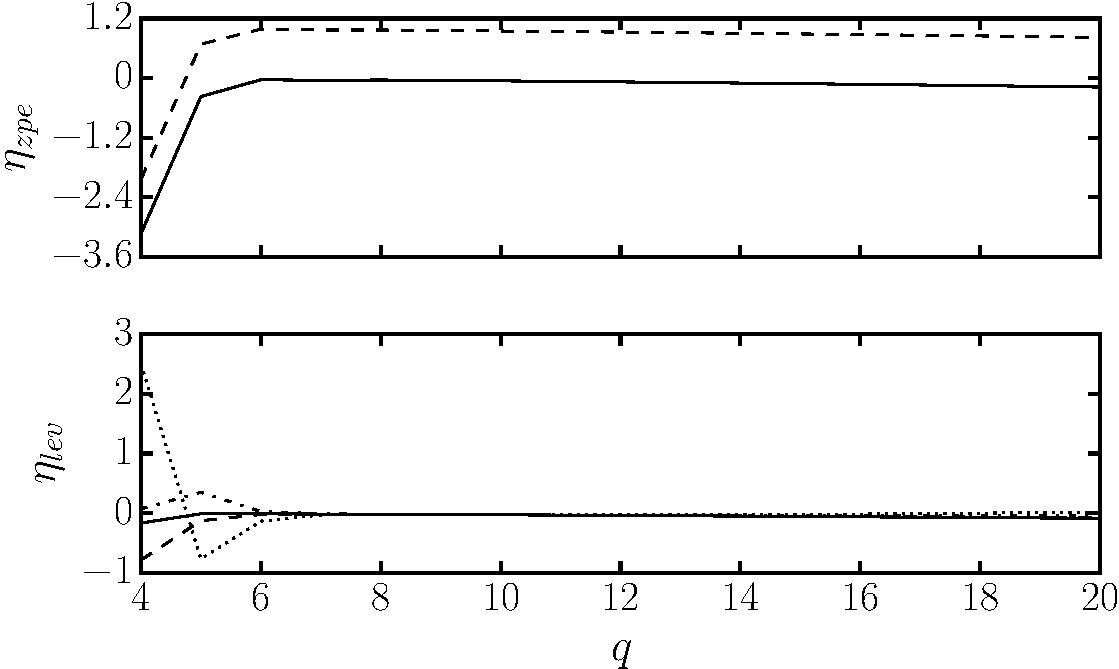
\includegraphics[width=.8\linewidth]{nonabcorr}
  % anc/scripts/nonabelian_fig.jl
  \caption{\emph{Top panel}: ``Zero-point energy" error, with (solid
curve, $\eta_{\text{zpe}}^{\text{nab}}$) and without (dashed line,
$\eta_{\text{zpe}}$) the shift from the off-diagonal matrix elements
of the Berry connection. Including just the first term in the sum
Eq.~\eqref{eq:shift} gives an identical curve to the one of
$\eta_{\text{zpe}}^{\text{nab}}$. The chosen trap strength is $\kappa
= 0.02 J$.  \emph{Bottom panel}: Level-spacing error, for the same
trap strength, considering $\beta = 0,1$ (solid curve), $\beta = 1,2$
(dashed curve), $\beta = 2,3$ (dashed-dotted curve) and $\beta = 3,4$
(dotted curve).}
  \label{fig:zpe}
\end{figure}

We turn now to the level-spacing error $\eta_{\text{lev}}$. This can
be expressed as
\begin{equation} \eta_{\text{lev}} = \frac{2\pi \alpha}{\kappa}
[E_{\text{ex}}(\beta) - E_{\text{ex}}(\beta - 1)] -1,
\end{equation} where we have used that the analytical level spacing
from Eq.~\eqref{eq:ladders} is simply $\kappa / 2\pi \alpha$.  We plot
the level-spacing error in the bottom panel of Fig.~\ref{fig:zpe} for
$\beta = 1, 2, 3$ and 4. As can be seen here, there is a large
variation in the errors at small $q$ due to the large
bandwidth~\cite{ozawa2014momhh}. On the other hand, we see that
$\eta_{\text{lev}} \ll 1$, for $q \gtrsim 6$, where the flat-band
approximation improves. In this regime, the level-spacing error is
much smaller than the zero-point error. This is because when the shift
from the off-diagonal matrix elements of the Berry connection
Eq.~\eqref{eq:shift} is approximately uniform over the MBZ at large
$q$, it just acts as a uniform energy shift on all the states in a
ladder with band index $n$. Consequently, this shift drops out of the
level spacing error between states, leaving only higher-order
band-mixing terms. From perturbation theory, it is expected that
mixing with other bands leads to a negative energy shift on states in
the lowest band, and indeed this can be seen in both
$\eta_{\text{zpe}}^{\text{nab}}$ and $\eta_{\text{lev}}$ in the small
negative errors found at large $q$.

\subsection{Driving and dissipation}\label{sec:driven-dissipation}

We now include in our model the driving and dissipation that are an
integral part of the proposed photonics experiment. We assume there
are uniform and local losses characterized by a loss rate $\gamma$,
and that the pump is monochromatic, with frequency $\omega_0$ and a
spatial profile $f_{m,n}$. Following the treatment of
Ref.~\cite{ozawa2014qhe}, we replace the bosonic creation and
annihilation operators with their expectation values, as can be
justified for a noninteracting system. The steady state evolution of
the photon-field amplitude in a cavity then follows that of the pump
as $a_{m,n}(t) = a_{m,n} e^{-i \omega_0 t}$. Combining Hamiltonian
evolution with pumping and losses, one arrives at a set of linear
coupled equations that can be solved numerically for the
steady-state\cite{cohen1992atom}:
%
\begin{multline}\label{eq:linear_problem} f_{m,n}
=J\left[e^{-i\phi_{m,n}^x}a_{m+1,n}+e^{i\phi_{m-1,n}^x}a_{m-1,n}
\right. \\
\left. +e^{-i\phi_{m,n}^y}a_{m,n+1}+e^{i\phi_{m,n-1}^y}a_{m,n-1}\right]
\\ +\left[\omega_{0}+i\gamma-\frac{1}{2}\kappa
\left((m-m_0)^{2}+(n-n_0)^{2}\right)\right]a_{m,n}
\end{multline} where we have reintroduced the position of the harmonic
trap centre $(m_0, n_0)$, although unless otherwise specified we set
$(m_0, n_0)=(0,0)$ in our simulations.

The expectation values $\abs{a_{m,n}}^2$ correspond to the number of
photons at site $(m,n)$, whereas the intensity spectrum is given by
their total sum $\sum_{m,n} |a_{m,n}|^2$ as a function of pump
frequency $\omega_0$. These observables can be directly related to the
eigenstates of the Hamiltonian in Eq.~\eqref{eq:model}. Firstly, the
different eigenmodes of a driven-dissipative system will appear as
peaks in the transmission and/or absorption spectra under a coherent
pump~\cite{carusotto2013fluids}. The resonance peaks will be broadened
by the decay rate $\gamma$, while the area of the peaks will depend on
the overlap between the spatial amplitude profile of the pump and the
underlying eigenstate of $\mathcal{H}$ at that energy.

Secondly, when the pump frequency is set on resonance with a given
mode, the intensity profiles in both real- and momentum-space
reproduce the wave function of that
mode~\cite{carusotto2013fluids}. This corresponds respectively to
measuring the near-field and far-field spatial emission of photons
from the cavity array. We note that the far-field emission is simply
the Fourier-transform of the real-space wave function and so will be a
function of crystal momentum defined in the full BZ. To reach the MBZ,
a further processing step is required; for example, if the
Harper-Hofstadter Hamiltonian is in the Landau gauge and if we choose
a magnetic unit cell of $q$ plaquettes along $\hat{x}$, the
appropriate transformation takes a particularly simple
form~\cite{price2014magnetic}:
%
\begin{equation} \label{eq:trans} \sum_n
\abs{\psi_n(\vt{p}_\mathrm{MBZ})}^2 = \sum_j
\abs{\psi(\vt{p}_\mathrm{BZ} = \vt{p}_\mathrm{MBZ}- j\vt{G})}^2 ,
\end{equation}
%
where $\psi_n(\vt{p}_\mathrm{MBZ})$ is the wave function coefficient
in the MBZ, while $\psi(\vt{p}_\mathrm{BZ})$ is that in the original
BZ. In this expression, $j$ is an integer, while $\vt{G} = (2\pi/q)
\hat{\vt{p}}_x $ is the magnetic reciprocal lattice vector, where the
factor of $q$ is due to the enlarged magnetic unit cell. We note that
for other magnetic gauges or for other choices of the magnetic unit
cell, this transformation will in general be more complicated. In this
sense, we call this choice of magnetic unit cell, a ``natural" choice
when the Harper-Hofstadter Hamiltonian is in the Landau gauge.  In the
rest of the article, we denote the momentum in the original BZ as
$\mathbf{p}$, and that in the MBZ as $\mathbf{p}^0$.

\section{Results and discussion}
\label{sec:results}

\subsection{Pumping and gauge-dependent effects}
\label{sec:selection}

\begin{figure}[tb]\centering
  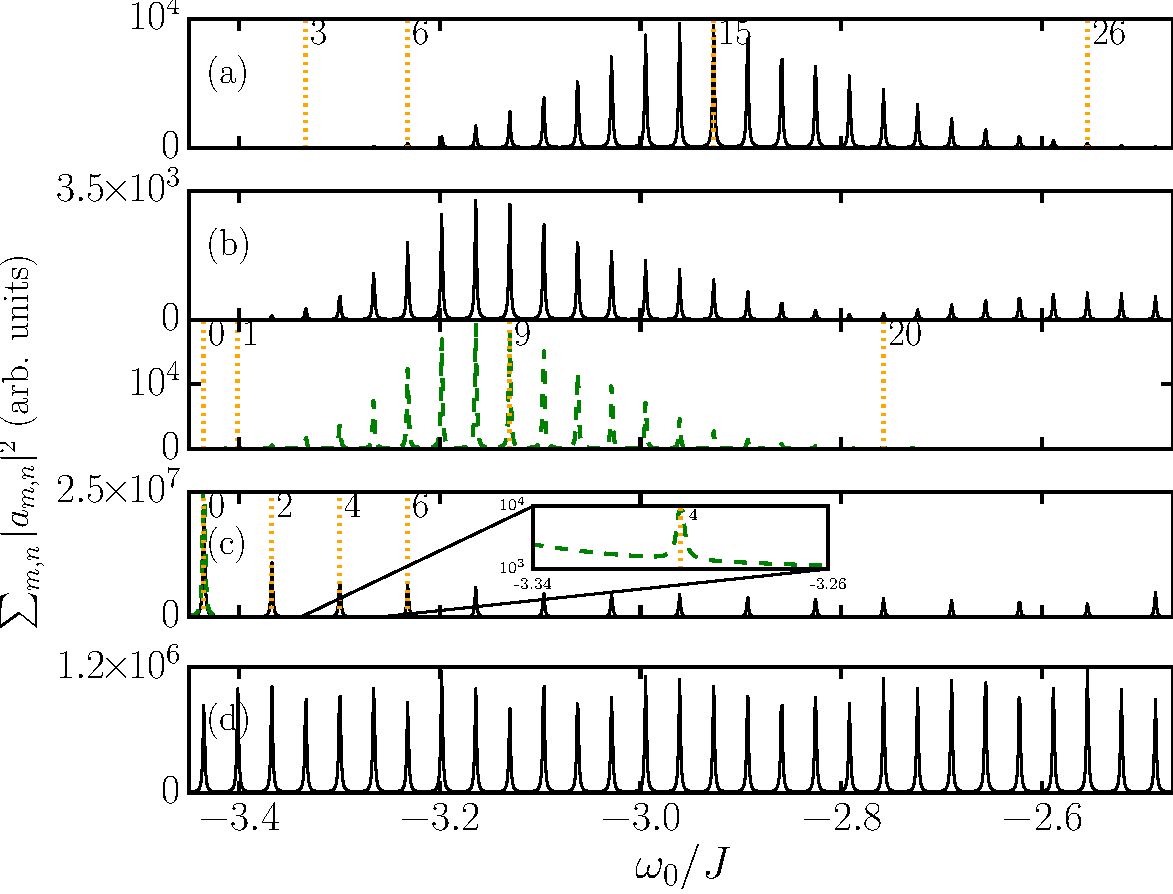
\includegraphics[width=\linewidth]{selection}
  % anc/scripts/selection_fig.jl
  \caption{Intensity spectra for different pumping conditions: (a)
pumping the single site (5,5), (b) pumping with a Gaussian profile
centered at site (5,5) with width $\sigma=1$, (c) homogeneous pumping
across all lattice sites and (d) pumping with a random phase across
all lattice sites. These results were obtained by numerical solving
Eq.~\eqref{eq:linear_problem} for the steady-state in a lattice of $N
\times N = 45 \times 45$ sites, with $\kappa = 0.02 J$, $\gamma =
0.001 J$ and $\alpha = 1/11$.  Black (solid) curves correspond to
using the Landau gauge while green (dashed) ones to the symmetric
gauge. The dotted vertical lines (with labels indicating the value of
$\beta$) mark the states which were selected for later analysis. The
spectra in panels (a) and (d) are identical for both gauges.}
  \label{fig:pumping_schemes}
\end{figure}

As introduced above, spectroscopic measurements can be used in a
driven-dissipative photonics experiment to study the trapped
Harper-Hofstadter model and hence toroidal Landau levels in momentum
space. In this section, we focus on the effects of the pumping,
exploring how different pumping schemes excite the eigenstates with
different weights. We find that such spectroscopic measurements are
sensitive to the underlying synthetic magnetic gauge chosen in a given
implementation of the Harper-Hofstadter Hamiltonian.

To best illustrate these gauge-dependent effects, we present the
results of numerically solving Eq.~\eqref{eq:linear_problem} for the
steady-state in a large lattice of $N \times N = 45 \times 45$ sites,
with $\kappa = 0.02 J$, $\gamma = 0.001 J$ and $\alpha = 1/11$.  These
parameters are chosen to highlight the key features of different
pumping schemes; we will present numerical results for a more
realistic experimental system in Section \ref{sec:experiment}.  The
numerical code was written in \textsc{Julia}~\cite{bezanson2014julia}
and is available in appendix~\ref{sec:source-code-landau}.

The intensity spectrum of the steady-state as a function of pump
frequency is shown in Fig.~\ref{fig:pumping_schemes}, where we compare
results for both the Landau and symmetric gauge for four pumping
schemes, discussed in turn below. For simplicity we limit ourselves to
pump frequencies located between the two lowest-lying
Harper-Hofstadter bands of the untrapped system. This allows us to
focus only on states within the first ladder of the trapped system
(Eq.~\eqref{eq:ladders} with $n = 0$). At higher energies, the clear
identification of states is more difficult as more than one ladder of
toroidal Landau levels can overlap, as shown, for example, in
Section~\ref{sec:experiment}.

{\em{Single-site pumping--}}The first and simplest case that we
consider is that of pumping a single site $f_{m,n} = \delta_{m,m_0}
\delta_{n,n_0}$ at an off-center lattice site. These results are shown
in Fig.~\ref{fig:pumping_schemes} panel (a), where the uniform energy
spacing of the toroidal Landau levels can be clearly observed. For
this pumping scheme, we find no significant differences between the
spectra for the Landau or symmetric gauge. This is to be expected as
changing the gauge is equivalent to changing the relative phase
between different sites, but as we are only pumping one site, this
phase difference is unimportant.

Instead, for both magnetic gauges, we see that the peak height is very
small for low energy states, rising to a maximum as energy increases,
before decreasing once more. This behaviour can be understand by
considering the form of the real space wavefunctions of $\mathcal{H}$.
In real space, the eigenstates are rings of finite width which
increase in radius as the energy increases (as can be seen in
Fig.~\ref{fig:delta_real_sp}). Analytically, we can predict how the
ring radius scales with energy by remembering that the term
$(\beta + 1/2) \kappa |\Omega_n|$ in Eq.~\eqref{eq:ladders} is the
momentum-space kinetic energy $\frac{\kappa}{2}r^2$ where
$r = i\nabla_{\mathbf{p}} + \mathcal{A}_{0, 0}(\mathbf{p})$ is the
physical position operator in the lowest band. From this, we deduce
that $r^2 \approx \frac{1}{\pi} q \beta$, as can be confirmed
numerically. Therefore, if one pumps an off-center site, there will
only be a limited range of rings that will have radii that will
overlap with the pump spot and so be excited. Here, we have set the
pump spot to be at position $(5,5)$, and from the above scaling, the
toroidal Landau level that best overlaps with this pump will have a
quantum number $\beta \approx 14$, which is in good agreement with the
numerical results shown in Fig.~\ref{fig:pumping_schemes} (a).

\begin{figure}[tb] \centering
  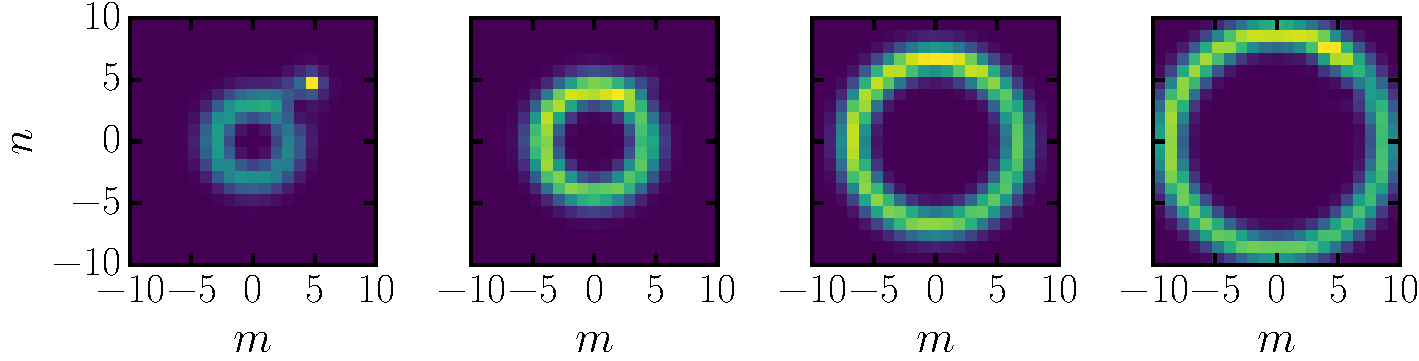
\includegraphics[width=0.9\linewidth]{real}
  % anc/scripts/selection_fig.jl
  \caption{Real space reconstruction of the states $\beta=3$, 6, 15
and 26 of Fig.~\ref{fig:pumping_schemes}(a).}
  \label{fig:delta_real_sp}
\end{figure}

{\em{Gaussian pumping--}} We now consider a Gaussian pump as the next
logical step up in complexity from a single-site pump. This has the
form $f_{m,n} = \exp- \frac{1}{2\sigma^2} \left[(m-m')^2 + (n-n')^2
\right]$, and we choose $\sigma =1$ and for the pump centre to be at
$(m',n') = (5,5)$, as for single-site pumping. The results are shown
in Fig.~\ref{fig:pumping_schemes} (b). The main effect is, as
expected, that more states become visible in both the low- (smaller
$\beta$) and high-energy (larger $\beta$) sections of the
spectrum. This is because the pump has a greater spatial width and so
overlaps with a larger range of real-space eigenstates.

However, we can also see that the intensity spectrum now depends on
the underlying magnetic gauge, as the phase of the eigenstates is
important. In particular, more high-energy peaks can be seen for the
Landau gauge than for the symmetric gauge. This can be most easily
understood by noting that in momentum space, the symmetric-gauge
states also have a ring-like structure (see bottom panel of
Fig.~\ref{fig:hom_mom_sp}), where the ring radius increases with
$\beta$. To see this, we note that, in the symmetric gauge, the
real-space wavefunctions have a phase which winds around the ring as
$e^{i\beta \phi}$ where $\phi$ is the polar angle around the
ring. This phase-winding sets the radius of the rings in momentum
space as $p^2 \approx \pi \frac{\beta}{q}$; a scaling that can be
confirmed numerically and seen in Fig.~\ref{fig:hom_mom_sp}, bottom
panel. (The white spot close to the edges of the rings in these
figures is due to destructive interference with the pump.)  As the
Fourier transform of the Gaussian pump is again a Gaussian, it follows
that only a limited range of low-energy symmetric-gauge momentum-space
states will have a good overlap with the pump. The high energy portion
of the spectrum is therefore washed out compared to its Landau gauge
counterpart, where states have higher amplitude close to the centre of
the BZ and so better overlap with the pump.

\begin{figure}[tb]\centering
  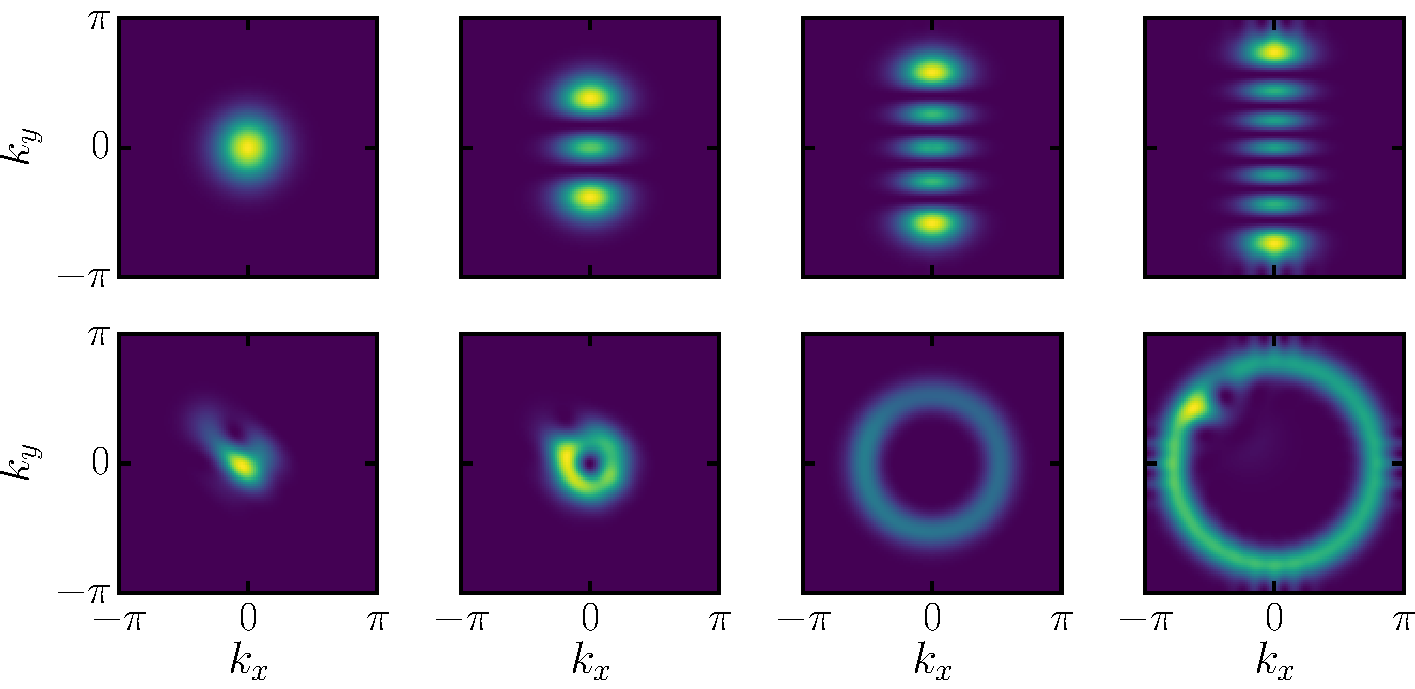
\includegraphics[width=0.9\linewidth]{momentum}
  % anc/scripts/selection_fig.jl
  \caption{Momentum space reconstruction of the eigenstates. \emph{Top
row}: states corresponding to $\beta=0$, 2, 4 and 6 in
Fig.~\ref{fig:pumping_schemes}(c), using the Landau gauge.
\emph{Bottom row}: states corresponding to $\beta=0$, 1, 9 and 20 in
Fig.~\ref{fig:pumping_schemes}(b), using the symmetric gauge.}
  \label{fig:hom_mom_sp}
\end{figure}

Before continuing, we also note that for sufficiently large values of
$\beta$ the symmetric-gauge rings in momentum space will increase to
the point where they touch the BZ boundaries. When this occurs,
self-interference patterns appear in the wave function as shown for
example in Fig.~\ref{fig:torus_edge}. The extra ring-like structures
appearing for $\beta \geq 30$ in Fig.~\ref{fig:torus_edge} are due to
the close proximity of states pertaining to other ladders with $n
>0$. Note that in order to excite such high-energy states, we have
used a pump with a homogeneous amplitude and a random onsite phase, as
will be presented in the fourth pumping case below.

{\em{Homogeneous pumping with uniform phase--}} If we now take the
limit of a very wide Gaussian, we reach a homogeneous pump profile
extended over all lattice sites. The results for this pumping scheme
are shown in panel (c) of Fig.~\ref{fig:pumping_schemes}. Now $f_{m,n}
= f$, and we see that the intensity spectrum is strongly
magnetic-gauge dependent. In the Landau gauge, firstly, there are
visible peaks for only half of the states. This can be understood by
noting that a homogeneous pump in real space is a $\delta$ function in
momentum space centered in the middle of the BZ. If we consider the
Landau-gauge eigenstates in the full BZ, as shown in the top row of
Fig.~\ref{fig:hom_mom_sp}, we see that the states with an even value
of $\beta$ have an even number of nodes, with a lobe at the BZ
center. Conversely, the states with odd values of $\beta$ have an odd
number of nodes, including one at the BZ center. (These feature can be
related back to the properties of the Hermite polynomials in the
analytical eigenstates in the MBZ Eq.~\eqref{eq:chi}.) Consequently,
only states with even values of $\beta$ have a good overlap with the
pump, and the intensity spectrum contains half the expected peaks, now
separated by twice the toroidal Landau level energy spacing.

In the symmetric gauge, secondly, we find only one out of every four
states for homogeneous pumping, as can be seen in the inset of
Fig.~\ref{fig:pumping_schemes} (c). This is due to the fact that, on a
square lattice, the angular momentum is conserved modulo 4, respecting
the 4-fold rotational symmetry. The peak intensity gets smaller for
larger $\beta$ because of the diminishing overlap of the localized
central pump with the increasing momentum-space ring discussed above.

\begin{figure}[tb] \centering
  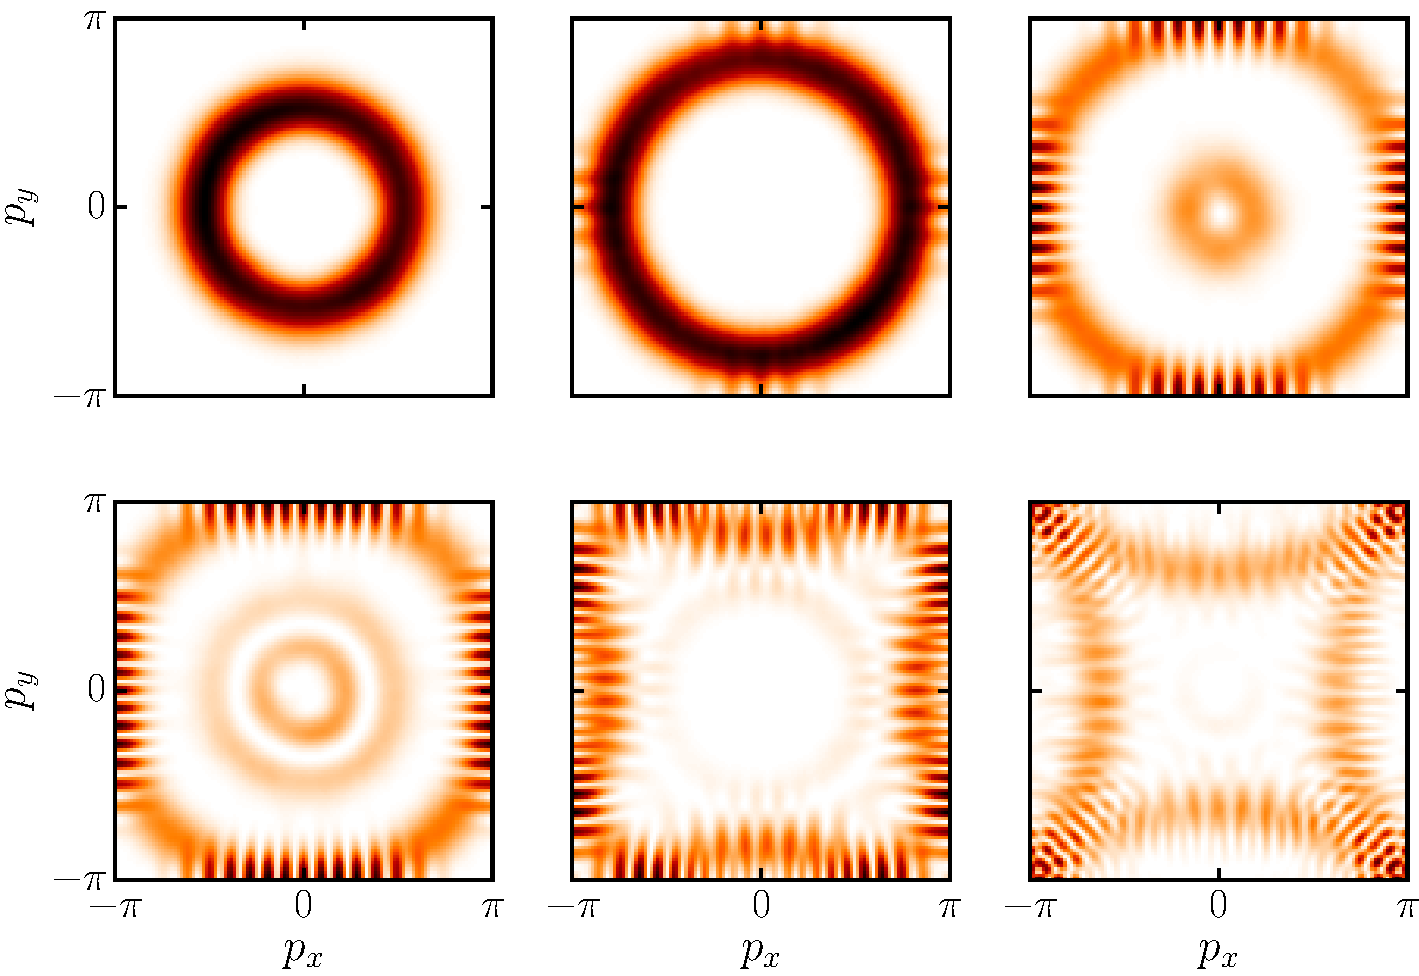
\includegraphics[width=.7\linewidth]{sym_ring}
  % anc/scripts/torus_edge_fig.jl
  \caption{Momentum space reconstruction of the eigenstates in the
full BZ, using the symmetric gauge and homogeneous pumping with a
random on-site phase. \emph{Top row}: states corresponding to $\beta =
9, 20, 30$.  \emph{Bottom row}: states corresponding to $\beta = 38,
59, 99$. Parameters are the same as in
Fig.~\ref{fig:pumping_schemes}.}
  \label{fig:torus_edge}
\end{figure}


{\em{Homogeneous pumping with a random on-site phase --}} As the
fourth scheme, we consider a pump with a uniform amplitude over the
lattice but a random site-dependent phase $\phi_{m,n}$:
$f_{m,n}=fe^{i\phi_{m,n}}$. The phases are chosen from a random
uniform distribution, and have values in the interval $[0,2\pi)$. The
bottom panel of Fig.~\ref{fig:pumping_schemes} was obtained by
averaging over 100 distinct realizations of these random phases. This
results in a relatively even intensity distribution, for both gauges,
where we can associate a peak to each toroidal Landau level in this
energy window. While such a pumping scheme would therefore be the best
way to excite all the eigenstates and to fully probe the
momentum-space physics, we note that this would also be difficult to
achieve in an experiment.
%
\begin{figure}[htb] \centering
  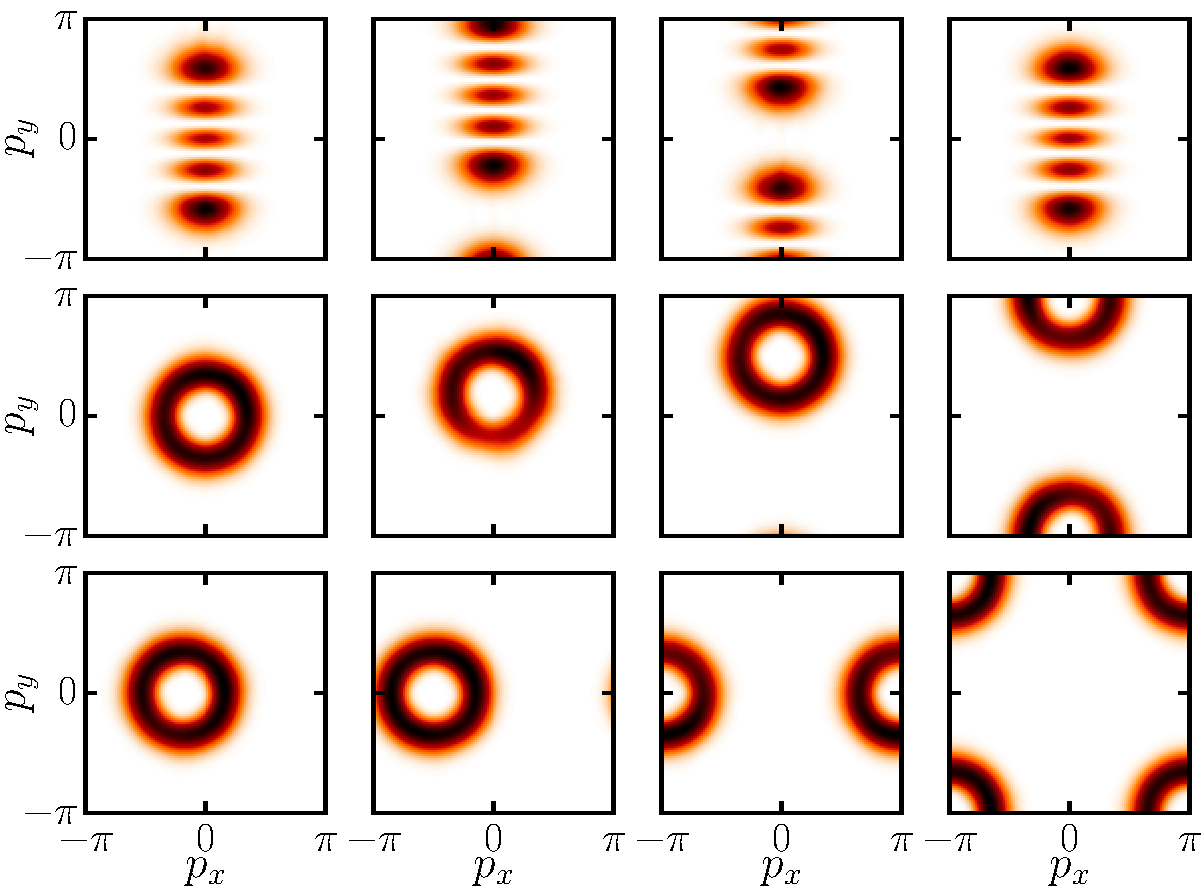
\includegraphics[width=.8\linewidth]{fringe_trap}
  % anc/scripts/torus_edge_fig.jl
  \caption{Momentum space reconstruction of the eigenstates in the
full BZ, using the Landau (top row) and symmetric gauge (middle and
bottom row) and a spatially homogeneous pump with a random on-site
phase. We have considered the state $\beta = 4$ for different trap
positions $(m_0, n_0)$. For the top and middle rows, we have (from
left to right): (0,0) (trap in the center), (2,0), (5.5,0) and (11,0),
whereas for the bottom row we chose the positions (0,2), (0,5.5),
(0,11) and (11,11). Parameters are the same as in
Fig.~\ref{fig:pumping_schemes}.}
  \label{fig:moving_trap}
\end{figure}
%
\begin{figure}[htb] \centering
  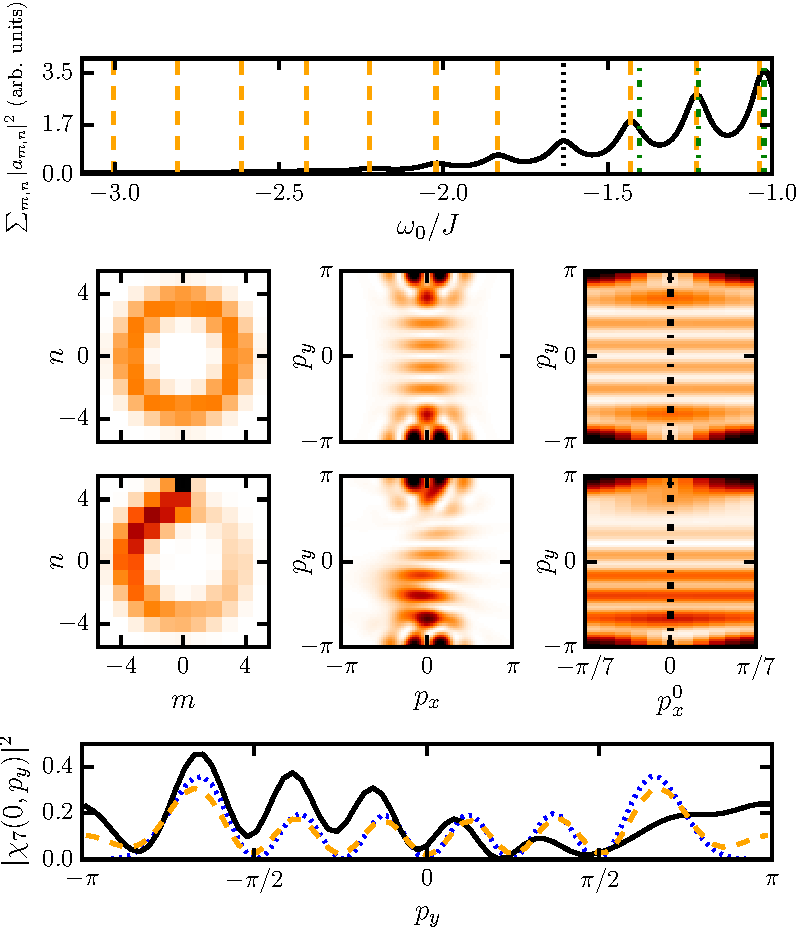
\includegraphics[width=.7\linewidth]{exp_fig}
  % anc/scripts/experimental_fig.jl
  \caption{\emph{Top row}: Intensity spectrum for a small lattice of
    $11 \times 11$ sites, with $\gamma = 0.05 J$, $\kappa = 0.2 J$ and
    $\alpha=1/7$.  \emph{Second row}: Profile of the $\beta=7$ state
    in real space (left), momentum space (center) and the population
    over bands in the MBZ (right) for the conservative system.
    \emph{Third row}: Reconstruction of the $\beta=7$ mode
    wavefunction in real space (left), momentum space (center) and the
    population over bands in the MBZ (right) obtained in the
    driven-dissipative system by pumping at $\omega_0 = -1.63 J$, on
    resonance with the desired mode (black dotted line in the top
    panel).  The $\delta$-like pump at (0,5) is visible as a dark
    square in the left panel.  \emph{Bottom row}: Slice along the
    $p_x^0 = 0$ line in the MBZ (solid black line), compared to the
    analytical prediction of Eq.~\eqref{eq:chi}, $|\chi_7(0,p_y)|^2$
    (blue dotted line) and to the population over bands for the
    nondissipative system (dashed orange line).}
  \label{fig:exp}
\end{figure}

Before continuing, we give a final example of an interesting
gauge-dependent effect that could be studied experimentally in this
system. Unlike the physics discussed above, this is not directly
related to the pumping but instead to the behaviour of the wave
function under a change in the centre of the harmonic trap $(m_0,
n_0)$. As derived in Ref. ~\cite{ozawa2014momhh}, moving the harmonic
trap in space changes the boundary conditions on the wave function in
the MBZ. We note that although this derivation was made explicitly for
the magnetic Landau gauge in the MBZ, numerically we observe here that
this physics is also seen in the full BZ in both gauges.  As shown
in Fig.~\ref{fig:moving_trap}, a shift in the harmonic trap centre in
one direction shifts the observed momentum-space pattern in the
perpendicular direction. This behaviour can be understood as a
realisation of Laughlin's {\em Gedankenexperiment} for the quantum
Hall effect but now in momentum space~\cite{ozawa2014momhh}. As we
observe, the momentum-space wave function returns to itself after the
harmonic trap has been moved $q$ lattice sites for the magnetic Landau
gauge but $2q$ lattice sites for the magnetic symmetric gauge,
reflecting the underlying translational symmetry of $\mathcal{H}_0$ in
the two different gauges.


\subsection{Results for realistic experimental parameters}
\label{sec:experiment}

We now present numerical results for system parameters within current
experimental reach, to demonstrate that the essential characteristics
of toroidal Landau levels could be probed experimentally for the first
time in photonics. We choose a small lattice of only $11 \times 11$
sites, with losses of $\gamma = 0.05 J$; this loss rate is in the same
range as those present in the experiment of
Ref.~\cite{hafezi2013imaging}. Such a large loss rate broadens the
peaks in the intensity spectrum, making closely-spaced eigenenergies
harder to resolve. From Eq.~\eqref{eq:ladders}, we see that the level
spacing is given by $\frac{\kappa}{2\pi\alpha}$, and so we can
increase the energy spacing by applying a stronger harmonic potential,
chosen here as $\kappa = 0.2 J$. Increasing the strength of the
harmonic trap improves our flat-band approximation, but weakens the
single-band approximation. To compensate for this, we consider a
larger value of $\alpha = 1/7$, for which the larger band-gap $(E_1 -
E_0)$ reduces band-mixing effects.

As in the experiment of Ref.~\cite{hafezi2013imaging}, we work in the
Landau gauge for the Harper-Hofstadter Hamiltonian, with hopping
phases given by $\phi = (0, 2\pi\alpha m)$. In order to model the
experimental pumping scheme where light was injected into a single
resonator at the edge of the system via an external integrated
waveguide~\cite{hafezi2013imaging}, we consider a localized pump on a
single site situated on the upper border of the system at
$(m_0,n_0)= (0,5)$.  The corresponding intensity spectrum is shown in
the 1st row of Fig.~\ref{fig:exp}. Apart from the expected broadening
due to larger losses, the peaks observed correspond well to the
expected eigenenergies.  As discussed above, single-site pumping
limits the number of visible peaks, as the heights of the peaks at
low-energies are suppressed due to the poor overlap of the real-space
eigenstate with the pump position. However, as this pumping scheme is
closest to that used in experiments, we emphasise that even in this
case, enough peaks can be observed to extract quantitative
measurements of the toroidal Landau level spacing. The orange vertical
(dashed) lines show the first ladder of eigenstates of $\mathcal{H}$
from Eq.~\eqref{eq:model}. We also note that here for frequencies
larger than $-1.5 J$, we also start to see states from the second
ladder $\epsilon_{1,\beta}$ (see Eq.~\eqref{eq:ladders}), which are
depicted as green vertical dash-dotted lines. Their proximity to the
first ladder states means they cannot be easily resolved as separate
peaks in the dissipative spectrum.

Setting the pump frequency at the energy indicated by the black dotted
line, we plot the numerical near- and far-field emission in the left
and center panels of the 3rd row of Fig.~\ref{fig:exp}. This
corresponds to the wave function in real space and in the full BZ,
respectively. By applying the transformation in Eq.~\eqref{eq:trans}, we
can also map the wave function in the full BZ to the population over
bands in the MBZ, as shown in the right panel of the 3rd row of
Fig.~\ref{fig:exp}. For comparison, we plot these quantities for the
corresponding numerical eigenstate of $\mathcal{H}$
Eq.~\eqref{eq:model} in the second row of Fig.~\ref{fig:exp}, for
which there is no pumping and dissipation.

We find very good qualitative agreement between the numerical results
in the MBZ and the analytical toroidal Landau level Eq.~\eqref{eq:chi}
with $\beta=7$, as expected. We can make a quantitative comparison with
this analytical eigenstate by taking a slice along the dash-dotted
vertical lines ($p_x^0 = 0$) in the right column of rows 2 and 3;
these cuts are shown in the bottom panel of Fig.~\ref{fig:exp} along
with a dotted blue curve indicating the analytical eigenstate. As can
be seen, there is excellent agreement between the numerics without
driving and dissipation and the analytical result. We have checked
that reducing $\kappa$ makes this fit even better, pointing towards
band-mixing effects. Introducing pumping and dissipation distorts the
eigenstate, but many characteristic features are still clearly
observable.

It is particularly interesting to note that in the driven-dissipative
steady-state in real space, shown in the left panel of the 3rd row of
Fig.~\ref{fig:exp}, the photon distribution breaks the rotational
symmetry of the ring eigenstate. While this can be physically
understood as a decaying cyclotron orbit with an inverse lifetime set
by $\gamma$, in terms of eigenmodes the exponential decay (and more
generally the breaking of the rotational symmetry) results from the
interference of several modes which overlap in frequency due to the
relatively large value of $\gamma$.  In the same way that real-space
Landau levels give rise to real-space cyclotron orbits under the
effect of the magnetic field, the observation of momentum-space Landau
levels can provide clear evidence of a cyclotron orbit in momentum
space under the effect of the Berry curvature, whose effect is indeed
that of a momentum-space magnetic field.

Finally, we briefly summarize how one can practically measure the
contribution $\delta E_0$ from the off-diagonal matrix elements of the
Berry connection (see Eq.~\eqref{eq:shift}) from the intensity
spectrum. Starting from an experimental spectrum, one first needs to
select a particular peak and determine its $\beta$ label by comparing
the MBZ reconstruction with the analytical result. The distance
between two neighbouring peaks gives the level spacing $\kappa
\abs{\Omega_0}$. Finally, to separate the shift $\delta E_0$ from the
Harper-Hofstadter ground state energy $E_0$ in Eq.~\eqref{eq:ladders},
one can make use of the fact that the former depends on the trap
strength $\kappa$, while the latter does not. Preparing two otherwise
identical samples with different trap strengths and subtracting the
ground state energy will then allow for a direct measurement of the
contribution from the off-diagonal matrix elements of the Berry
connection.

\section{Conclusion}
\label{sec:conclusion}

In conclusion, we have shown that the observation of toroidal Landau
levels in momentum space is within experimental reach for
state-of-the-art driven-dissipative photonic systems. Our proposal
combines the recent realisation of the Harper-Hofstatder model in an
array of silicon-based coupled ring resonators in
Ref.~\cite{hafezi2013imaging}, with a harmonic potential, which could
be introduced through a spatial modulation of the resonator size. We
have presented numerical results to show that even for very small
lattices, in the presence of driving and strong dissipation, key
characteristics of the toroidal Landau levels can still be
extracted. This would be a first direct investigation of analogue
magnetic eigenstates in momentum space.

We have also emphasised that the proposed photonics experiment would
be able to highlight a momentum-space analog of the cyclotron motion
as well as to measure the energy shift due to the off-diagonal matrix
elements of the Berry connection, which, as these are inter-band
geometrical properties, are hard to access by other means. We have
also discussed how the spectroscopic measurements presented here are
sensitive to the specific synthetic magnetic gauge implemented in an
experiment.

Finally, an interesting outlook would be to include the effect of
photon-photon interactions in the model, as the degenerate ground
states predicted in~\cite{ozawa2014momhh} for a weakly-interacting
trapped Harper-Hofstadter model may lead to interesting nonlinear
dynamical features. In the longer run, when the synthetic gauge field
is combined with strong interactions, one can hope to observe the
hallmarks of fractional quantum Hall
physics~\cite{umucalilar2012fractional,hafezi2013non}.

\begin{subappendices}

  \section{Source code}\label{sec:source-code-landau}
  %
  This appendix contains \textsc{Julia} 0.3 source code for the
numerical simulations used to produce the figures appearing in
Chapter~\ref{cha:landau}. Sec.~\ref{subsec:bp} contains the main
program module, defining the functions used in simulations, while
Sec.~\ref{subsec:hh} contains the module for constructing and
diagonalizing the Harper-Hofstadter Hamiltonian.
  %
The figures are plotted using the \textsc{matplotlib} \textsc{Python}
library v1.4.3, as follows: Sec.~\ref{subsec:nonabelian} contains the
code for Fig.~\ref{fig:zpe}; Sec.~\ref{subsec:selection} produces
Figs.~\ref{fig:pumping_schemes}, \ref{fig:delta_real_sp},
and~\ref{fig:hom_mom_sp}; Sec.~\ref{subsec:torus-edge} produces
Figs.\ref{fig:torus_edge} and~\ref{fig:moving_trap} and finally,
Sec.~\ref{subsec:experimental} produces Fig.~\ref{fig:exp}.
  %
  %%%%%%%%%%%%%%%%%%%%%%%%%%%%%%%%%%%%%%%%%%%%%%%%%
% pygmentize -l julia -f latex -o BP.tex BP.jl  %
%%%%%%%%%%%%%%%%%%%%%%%%%%%%%%%%%%%%%%%%%%%%%%%%%

\subsection{BP.jl}\label{subsec:bp}
\begin{Verbatim}[commandchars=\\\{\}]
\PY{k}{module} \PY{n}{BP}
\PY{k}{using} \PY{n}{Polynomials}
\PY{k}{using} \PY{n}{Base}\PY{o}{.}\PY{n}{Test}
\PY{k}{type}\PY{n+nc}{ }\PY{n+nc}{WaveFunction}
    \PY{n}{N}\PY{p}{:}\PY{p}{:}\PY{k+kt}{Int}
    \PY{n}{int}\PY{p}{:}\PY{p}{:}\PY{k+kt}{Float64}
    \PY{n}{ψ}\PY{p}{:}\PY{p}{:}\PY{n}{Vector}\PY{p}{\PYZob{}}\PY{n}{Complex}\PY{p}{\PYZob{}}\PY{k+kt}{Float64}\PY{p}{\PYZcb{}}\PY{p}{\PYZcb{}}
\PY{k}{end}
\PY{n}{WaveFunction}\PY{p}{(}\PY{n}{S}\PY{p}{:}\PY{p}{:}\PY{n}{SparseMatrixCSC}\PY{p}{\PYZob{}}\PY{n}{Complex}\PY{p}{\PYZob{}}\PY{k+kt}{Float64}\PY{p}{\PYZcb{}}\PY{p}{,}\PY{k+kt}{Int64}\PY{p}{\PYZcb{}}\PY{p}{,}
             \PY{n}{ω}\PY{p}{:}\PY{p}{:}\PY{k+kt}{Float64}\PY{p}{,}\PY{n}{P}\PY{p}{:}\PY{p}{:}\PY{n}{Vector}\PY{p}{\PYZob{}}\PY{n}{Complex}\PY{p}{\PYZob{}}\PY{k+kt}{Float64}\PY{p}{\PYZcb{}}\PY{p}{\PYZcb{}}\PY{p}{)} \PY{o}{=}
                \PY{n}{WaveFunction}\PY{p}{(}\PY{n}{S}\PY{p}{,}\PY{n}{ω}\PY{p}{,}\PY{n}{P}\PY{p}{,}\PY{p}{:}\PY{n}{landau}\PY{p}{)}
\PY{n}{WaveFunction}\PY{p}{(}\PY{n}{S}\PY{p}{:}\PY{p}{:}\PY{n}{SparseMatrixCSC}\PY{p}{\PYZob{}}\PY{n}{Complex}\PY{p}{\PYZob{}}\PY{k+kt}{Float64}\PY{p}{\PYZcb{}}\PY{p}{,}\PY{k+kt}{Int64}\PY{p}{\PYZcb{}}\PY{p}{,}
             \PY{n}{ω}\PY{p}{:}\PY{p}{:}\PY{k+kt}{Float64}\PY{p}{,}\PY{n}{P}\PY{p}{:}\PY{p}{:}\PY{n}{Vector}\PY{p}{\PYZob{}}\PY{n}{Complex}\PY{p}{\PYZob{}}\PY{k+kt}{Float64}\PY{p}{\PYZcb{}}\PY{p}{\PYZcb{}}\PY{p}{,}\PY{n}{gauge}\PY{p}{:}\PY{p}{:}\PY{n}{Symbol}\PY{p}{)}
                 \PY{o}{=} \PY{n}{WaveFunction}\PY{p}{(}\PY{n}{S}\PY{p}{,}\PY{n}{ω}\PY{p}{,}\PY{n}{P}\PY{p}{,}\PY{n}{gauge}\PY{p}{,}\PY{l+m+mi}{1}\PY{o}{/}\PY{l+m+mi}{11}\PY{p}{,}\PY{l+m+mf}{0.001}\PY{p}{,}\PY{l+m+mf}{0.02}\PY{p}{,}\PY{l+m+mf}{0.}\PY{p}{,}\PY{l+m+mf}{0.}\PY{p}{)}
\PY{n}{WaveFunction}\PY{p}{(}\PY{n}{S}\PY{p}{:}\PY{p}{:}\PY{n}{SparseMatrixCSC}\PY{p}{\PYZob{}}\PY{n}{Complex}\PY{p}{\PYZob{}}\PY{k+kt}{Float64}\PY{p}{\PYZcb{}}\PY{p}{,}\PY{k+kt}{Int64}\PY{p}{\PYZcb{}}\PY{p}{,}
             \PY{n}{ω}\PY{p}{:}\PY{p}{:}\PY{k+kt}{Float64}\PY{p}{,}\PY{n}{P}\PY{p}{:}\PY{p}{:}\PY{n}{Vector}\PY{p}{\PYZob{}}\PY{n}{Complex}\PY{p}{\PYZob{}}\PY{k+kt}{Float64}\PY{p}{\PYZcb{}}\PY{p}{\PYZcb{}}\PY{p}{,}\PY{n}{gauge}\PY{p}{:}\PY{p}{:}\PY{n}{Symbol}\PY{p}{,}
             \PY{n}{α}\PY{p}{:}\PY{p}{:}\PY{k+kt}{Float64}\PY{p}{,}\PY{n}{γ}\PY{p}{:}\PY{p}{:}\PY{k+kt}{Float64}\PY{p}{,}\PY{n}{κ}\PY{p}{:}\PY{p}{:}\PY{k+kt}{Float64}\PY{p}{)} \PY{o}{=}
                 \PY{n}{WaveFunction}\PY{p}{(}\PY{n}{S}\PY{p}{,}\PY{n}{ω}\PY{p}{,}\PY{n}{P}\PY{p}{,}\PY{n}{gauge}\PY{p}{,}\PY{n}{α}\PY{p}{,}\PY{n}{γ}\PY{p}{,}\PY{n}{κ}\PY{p}{,} \PY{l+m+mf}{0.}\PY{p}{,} \PY{l+m+mf}{0.}\PY{p}{)}
\PY{k}{function}\PY{n+nf}{ }\PY{n+nf}{WaveFunction}\PY{p}{(}\PY{n}{S}\PY{p}{:}\PY{p}{:}\PY{n}{SparseMatrixCSC}\PY{p}{\PYZob{}}\PY{n}{Complex}\PY{p}{\PYZob{}}\PY{k+kt}{Float64}\PY{p}{\PYZcb{}}\PY{p}{,}\PY{k+kt}{Int64}\PY{p}{\PYZcb{}}\PY{p}{,}
                      \PY{n}{ω}\PY{p}{:}\PY{p}{:}\PY{k+kt}{Float64}\PY{p}{,}\PY{n}{P}\PY{p}{:}\PY{p}{:}\PY{n}{Vector}\PY{p}{\PYZob{}}\PY{n}{Complex}\PY{p}{\PYZob{}}\PY{k+kt}{Float64}\PY{p}{\PYZcb{}}\PY{p}{\PYZcb{}}\PY{p}{,}
                      \PY{n}{gauge}\PY{p}{:}\PY{p}{:}\PY{n}{Symbol}\PY{p}{,} \PY{n}{α}\PY{p}{:}\PY{p}{:}\PY{k+kt}{Float64}\PY{p}{,}\PY{n}{γ}\PY{p}{:}\PY{p}{:}\PY{k+kt}{Float64}\PY{p}{,}
                      \PY{n}{κ}\PY{p}{:}\PY{p}{:}\PY{k+kt}{Float64}\PY{p}{,} \PY{n}{m₀}\PY{p}{:}\PY{p}{:}\PY{k+kt}{Float64}\PY{p}{,} \PY{n}{n₀}\PY{p}{:}\PY{p}{:}\PY{k+kt}{Float64}\PY{p}{)}
    \PY{n}{N}\PY{p}{:}\PY{p}{:}\PY{k+kt}{Int} \PY{o}{=} \PY{n}{sqrt}\PY{p}{(}\PY{n}{length}\PY{p}{(}\PY{n}{P}\PY{p}{)}\PY{p}{)}
    \PY{n}{eval}\PY{p}{(}\PY{p}{:}\PY{p}{(}\PY{o}{\PYZdl{}}\PY{p}{(}\PY{n}{symbol}\PY{p}{(}\PY{n}{string}\PY{p}{(}\PY{l+s}{\PYZdq{}}\PY{l+s}{buildham\PYZus{}}\PY{l+s}{\PYZdq{}}\PY{p}{,} \PY{n}{gauge}\PY{p}{,} \PY{l+s}{\PYZdq{}}\PY{l+s}{!}\PY{l+s}{\PYZdq{}}\PY{p}{)}\PY{p}{)}\PY{p}{)}\PY{p}{)}\PY{p}{)}\PY{p}{(}\PY{n}{S}\PY{p}{,} \PY{n}{N}\PY{p}{,}\PY{n}{α}\PY{p}{,}\PY{n}{κ}\PY{p}{,}\PY{n}{γ}\PY{p}{,}
       \PY{n}{ω}\PY{p}{,}\PY{n}{m₀}\PY{p}{,}\PY{n}{n₀}\PY{p}{)}
    \PY{n}{X} \PY{o}{=} \PY{n}{S}\PYZbs{}\PY{n}{P}
    \PY{k}{return} \PY{n}{WaveFunction}\PY{p}{(}\PY{n}{N}\PY{p}{,}\PY{n}{sum}\PY{p}{(}\PY{n}{abs2}\PY{p}{(}\PY{n}{X}\PY{p}{)}\PY{p}{)}\PY{p}{,}\PY{n}{X}\PY{p}{)}
\PY{k}{end}
\PY{k}{type}\PY{n+nc}{ }\PY{n+nc}{ExactStates}
    \PY{n}{N}\PY{p}{:}\PY{p}{:}\PY{k+kt}{Int}
    \PY{n}{gauge}\PY{p}{:}\PY{p}{:}\PY{n}{Symbol}
    \PY{n}{νs}\PY{p}{:}\PY{p}{:}\PY{n}{Vector}\PY{p}{\PYZob{}}\PY{k+kt}{Float64}\PY{p}{\PYZcb{}}
    \PY{n}{states}\PY{p}{:}\PY{p}{:}\PY{n}{Matrix}\PY{p}{\PYZob{}}\PY{n}{Complex}\PY{p}{\PYZob{}}\PY{k+kt}{Float64}\PY{p}{\PYZcb{}}\PY{p}{\PYZcb{}}
\PY{k}{end}
\PY{n}{ExactStates}\PY{p}{(}\PY{n}{nev}\PY{p}{:}\PY{p}{:}\PY{k+kt}{Int}\PY{p}{,} \PY{n}{gauge}\PY{p}{:}\PY{p}{:}\PY{n}{Symbol}\PY{p}{)} \PY{o}{=} \PY{n}{ExactStates}\PY{p}{(}\PY{n}{nev}\PY{p}{,} \PY{n}{gauge}\PY{p}{,} \PY{l+m+mi}{45}\PY{p}{)}
\PY{n}{ExactStates}\PY{p}{(}\PY{n}{nev}\PY{p}{:}\PY{p}{:}\PY{k+kt}{Int}\PY{p}{,} \PY{n}{gauge}\PY{p}{:}\PY{p}{:}\PY{n}{Symbol}\PY{p}{,} \PY{n}{N}\PY{p}{:}\PY{p}{:}\PY{k+kt}{Int}\PY{p}{)} \PY{o}{=} \PY{n}{ExactStates}\PY{p}{(}\PY{n}{nev}\PY{p}{,}
   \PY{n}{gauge}\PY{p}{,} \PY{n}{N}\PY{p}{,} \PY{l+m+mi}{1}\PY{o}{/}\PY{l+m+mi}{11}\PY{p}{,} \PY{l+m+mf}{0.02}\PY{p}{,} \PY{l+m+mf}{0.}\PY{p}{,} \PY{l+m+mf}{0.}\PY{p}{)}
\PY{n}{ExactStates}\PY{p}{(}\PY{n}{nev}\PY{p}{:}\PY{p}{:}\PY{k+kt}{Int}\PY{p}{,} \PY{n}{gauge}\PY{p}{:}\PY{p}{:}\PY{n}{Symbol}\PY{p}{,} \PY{n}{N}\PY{p}{:}\PY{p}{:}\PY{k+kt}{Int}\PY{p}{,} \PY{n}{α}\PY{p}{:}\PY{p}{:}\PY{k+kt}{Float64}\PY{p}{,}
   \PY{n}{κ}\PY{p}{:}\PY{p}{:}\PY{k+kt}{Float64}\PY{p}{)} \PY{o}{=} \PY{n}{ExactStates}\PY{p}{(}\PY{n}{nev}\PY{p}{,} \PY{n}{gauge}\PY{p}{,} \PY{n}{N}\PY{p}{,} \PY{n}{α}\PY{p}{,} \PY{n}{κ}\PY{p}{,} \PY{l+m+mf}{0.}\PY{p}{,} \PY{l+m+mf}{0.}\PY{p}{)}
\PY{k}{function}\PY{n+nf}{ }\PY{n+nf}{ExactStates}\PY{p}{(}\PY{n}{nev}\PY{p}{:}\PY{p}{:}\PY{k+kt}{Int}\PY{p}{,} \PY{n}{gauge}\PY{p}{:}\PY{p}{:}\PY{n}{Symbol}\PY{p}{,} \PY{n}{N}\PY{p}{:}\PY{p}{:}\PY{k+kt}{Int}\PY{p}{,} \PY{n}{α}\PY{p}{:}\PY{p}{:}\PY{k+kt}{Float64}\PY{p}{,}
   \PY{n}{κ}\PY{p}{:}\PY{p}{:}\PY{k+kt}{Float64}\PY{p}{,} \PY{n}{m₀}\PY{p}{:}\PY{p}{:}\PY{k+kt}{Float64}\PY{p}{,} \PY{n}{n₀}\PY{p}{:}\PY{p}{:}\PY{k+kt}{Float64}\PY{p}{)}
    \PY{n}{M} \PY{o}{=} \PY{n}{spzeros}\PY{p}{(}\PY{n}{Complex}\PY{p}{\PYZob{}}\PY{k+kt}{Float64}\PY{p}{\PYZcb{}}\PY{p}{,} \PY{n}{N}\PY{o}{\PYZca{}}\PY{l+m+mi}{2}\PY{p}{,}\PY{n}{N}\PY{o}{\PYZca{}}\PY{l+m+mi}{2}\PY{p}{)}
    \PY{n}{eval}\PY{p}{(}\PY{p}{:}\PY{p}{(}\PY{o}{\PYZdl{}}\PY{p}{(}\PY{n}{symbol}\PY{p}{(}\PY{n}{string}\PY{p}{(}\PY{l+s}{\PYZdq{}}\PY{l+s}{buildhamexact}\PY{l+s}{\PYZdq{}}\PY{p}{,} \PY{n}{gauge}\PY{p}{,} \PY{l+s}{\PYZdq{}}\PY{l+s}{!}\PY{l+s}{\PYZdq{}}\PY{p}{)}\PY{p}{)}\PY{p}{)}\PY{p}{)}\PY{p}{)}\PY{p}{(}\PY{n}{M}\PY{p}{,} \PY{n}{N}\PY{p}{,}\PY{n}{α}\PY{p}{,}
       \PY{n}{κ}\PY{p}{,}\PY{n}{m₀}\PY{p}{,}\PY{n}{n₀}\PY{p}{)}
    \PY{p}{(}\PY{n}{d}\PY{p}{,} \PY{n}{v}\PY{p}{,} \PY{n}{nconv}\PY{p}{,} \PY{n}{niter}\PY{p}{,} \PY{n}{nmult}\PY{p}{,} \PY{n}{resid}\PY{p}{)} \PY{o}{=} \PY{n}{eigs}\PY{p}{(}\PY{n}{M}\PY{p}{,} \PY{n}{nev}\PY{o}{=}\PY{n}{nev}\PY{p}{,}
       \PY{n}{which}\PY{o}{=}\PY{p}{:}\PY{n}{SR}\PY{p}{,} \PY{n}{ritzvec}\PY{o}{=}\PY{n}{true}\PY{p}{)}
    \PY{k}{return} \PY{n}{ExactStates}\PY{p}{(}\PY{n}{N}\PY{p}{,} \PY{n}{gauge}\PY{p}{,} \PY{n}{real}\PY{p}{(}\PY{n}{d}\PY{p}{)}\PY{p}{,} \PY{n}{v}\PY{p}{)}
\PY{k}{end}
\PY{k}{function}\PY{n+nf}{ }\PY{n+nf}{getstate}\PY{p}{(}\PY{n}{s}\PY{p}{:}\PY{p}{:}\PY{n}{ExactStates}\PY{p}{,} \PY{n}{ω}\PY{p}{:}\PY{p}{:}\PY{k+kt}{Float64}\PY{p}{)}
    \PY{n}{i}\PY{p}{:}\PY{p}{:}\PY{k+kt}{Int} \PY{o}{=} \PY{n}{indmin}\PY{p}{(}\PY{n}{abs}\PY{p}{(}\PY{n}{s}\PY{o}{.}\PY{n}{νs} \PY{o}{.}\PY{o}{\PYZhy{}} \PY{n}{ω}\PY{p}{)}\PY{p}{)}
    \PY{k}{return} \PY{n}{reshape}\PY{p}{(}\PY{n}{s}\PY{o}{.}\PY{n}{states}\PY{p}{[}\PY{p}{:}\PY{p}{,}\PY{n}{i}\PY{p}{]}\PY{p}{,} \PY{p}{(}\PY{n}{s}\PY{o}{.}\PY{n}{N}\PY{p}{,} \PY{n}{s}\PY{o}{.}\PY{n}{N}\PY{p}{)}\PY{p}{)}
\PY{k}{end}
\PY{k}{function}\PY{n+nf}{ }\PY{n+nf}{getstate}\PY{p}{(}\PY{n}{s}\PY{p}{:}\PY{p}{:}\PY{n}{ExactStates}\PY{p}{,} \PY{n}{η}\PY{p}{:}\PY{p}{:}\PY{k+kt}{Int}\PY{p}{)}
    \PY{k}{return} \PY{n}{reshape}\PY{p}{(}\PY{n}{s}\PY{o}{.}\PY{n}{states}\PY{p}{[}\PY{p}{:}\PY{p}{,}\PY{n}{η}\PY{p}{]}\PY{p}{,} \PY{p}{(}\PY{n}{s}\PY{o}{.}\PY{n}{N}\PY{p}{,} \PY{n}{s}\PY{o}{.}\PY{n}{N}\PY{p}{)}\PY{p}{)}
\PY{k}{end}
\PY{k}{type}\PY{n+nc}{ }\PY{n+nc}{Spectrum}
    \PY{n}{N}\PY{p}{:}\PY{p}{:}\PY{k+kt}{Int}
    \PY{n}{gauge}\PY{p}{:}\PY{p}{:}\PY{n}{Symbol}
    \PY{n}{pump}\PY{p}{:}\PY{p}{:}\PY{n}{Vector}\PY{p}{\PYZob{}}\PY{n}{Complex}\PY{p}{\PYZob{}}\PY{k+kt}{Float64}\PY{p}{\PYZcb{}}\PY{p}{\PYZcb{}}
    \PY{n}{νs}\PY{p}{:}\PY{p}{:}\PY{n}{Vector}\PY{p}{\PYZob{}}\PY{k+kt}{Float64}\PY{p}{\PYZcb{}}
    \PY{n}{intensity}\PY{p}{:}\PY{p}{:}\PY{n}{Vector}\PY{p}{\PYZob{}}\PY{k+kt}{Float64}\PY{p}{\PYZcb{}}
    \PY{n}{states}\PY{p}{:}\PY{p}{:}\PY{n}{Vector}\PY{p}{\PYZob{}}\PY{n}{WaveFunction}\PY{p}{\PYZcb{}}
\PY{k}{end}
\PY{n}{Spectrum}\PY{p}{(}\PY{n}{ν}\PY{p}{:}\PY{p}{:}\PY{n}{Vector}\PY{p}{\PYZob{}}\PY{k+kt}{Float64}\PY{p}{\PYZcb{}}\PY{p}{,}\PY{n}{P}\PY{p}{:}\PY{p}{:}\PY{n}{Vector}\PY{p}{\PYZob{}}\PY{n}{Complex}\PY{p}{\PYZob{}}\PY{k+kt}{Float64}\PY{p}{\PYZcb{}}\PY{p}{\PYZcb{}}\PY{p}{)} \PY{o}{=}
   \PY{n}{Spectrum}\PY{p}{(}\PY{n}{ν}\PY{p}{,}\PY{n}{P}\PY{p}{,}\PY{p}{:}\PY{n}{landau}\PY{p}{)}
\PY{k}{function}\PY{n+nf}{ }\PY{n+nf}{Spectrum}\PY{p}{(}\PY{n}{ν}\PY{p}{:}\PY{p}{:}\PY{n}{Vector}\PY{p}{\PYZob{}}\PY{k+kt}{Float64}\PY{p}{\PYZcb{}}\PY{p}{,}\PY{n}{P}\PY{p}{:}\PY{p}{:}\PY{n}{Vector}\PY{p}{\PYZob{}}\PY{n}{Complex}\PY{p}{\PYZob{}}\PY{k+kt}{Float64}\PY{p}{\PYZcb{}}\PY{p}{\PYZcb{}}\PY{p}{,}
   \PY{n}{gauge}\PY{p}{:}\PY{p}{:}\PY{n}{Symbol}\PY{p}{)}
    \PY{n}{statevec} \PY{o}{=} \PY{n}{Array}\PY{p}{(}\PY{n}{WaveFunction}\PY{p}{,} \PY{n}{length}\PY{p}{(}\PY{n}{ν}\PY{p}{)}\PY{p}{)}
    \PY{n}{intvec} \PY{o}{=} \PY{n}{Array}\PY{p}{(}\PY{k+kt}{Float64}\PY{p}{,} \PY{n}{length}\PY{p}{(}\PY{n}{ν}\PY{p}{)}\PY{p}{)}
    \PY{n}{N}\PY{p}{:}\PY{p}{:}\PY{k+kt}{Int} \PY{o}{=} \PY{n}{sqrt}\PY{p}{(}\PY{n}{length}\PY{p}{(}\PY{n}{P}\PY{p}{)}\PY{p}{)}
    \PY{n}{A} \PY{o}{=} \PY{n}{spzeros}\PY{p}{(}\PY{n}{Complex}\PY{p}{\PYZob{}}\PY{k+kt}{Float64}\PY{p}{\PYZcb{}}\PY{p}{,} \PY{n}{N}\PY{o}{\PYZca{}}\PY{l+m+mi}{2}\PY{p}{,}\PY{n}{N}\PY{o}{\PYZca{}}\PY{l+m+mi}{2}\PY{p}{)}
    \PY{k}{for} \PY{p}{(}\PY{n}{i}\PY{p}{,}\PY{n}{ω}\PY{p}{)} \PY{k}{in} \PY{n}{enumerate}\PY{p}{(}\PY{n}{ν}\PY{p}{)}
        \PY{n}{statevec}\PY{p}{[}\PY{n}{i}\PY{p}{]} \PY{o}{=} \PY{n}{WaveFunction}\PY{p}{(}\PY{n}{A}\PY{p}{,} \PY{n}{ω}\PY{p}{,} \PY{n}{P}\PY{p}{,} \PY{n}{gauge}\PY{p}{)}
        \PY{n}{intvec}\PY{p}{[}\PY{n}{i}\PY{p}{]} \PY{o}{=} \PY{n}{statevec}\PY{p}{[}\PY{n}{i}\PY{p}{]}\PY{o}{.}\PY{n}{int}
    \PY{k}{end}
    \PY{k}{return} \PY{n}{Spectrum}\PY{p}{(}\PY{n}{N}\PY{p}{,} \PY{n}{gauge}\PY{p}{,} \PY{n}{P}\PY{p}{,} \PY{n}{ν}\PY{p}{,} \PY{n}{intvec}\PY{p}{,} \PY{n}{statevec}\PY{p}{)}
\PY{k}{end}
\PY{k}{function}\PY{n+nf}{ }\PY{n+nf}{Spectrum}\PY{p}{(}\PY{n}{ν}\PY{p}{:}\PY{p}{:}\PY{n}{Vector}\PY{p}{\PYZob{}}\PY{k+kt}{Float64}\PY{p}{\PYZcb{}}\PY{p}{,}\PY{n}{P}\PY{p}{:}\PY{p}{:}\PY{n}{Vector}\PY{p}{\PYZob{}}\PY{n}{Complex}\PY{p}{\PYZob{}}\PY{k+kt}{Float64}\PY{p}{\PYZcb{}}\PY{p}{\PYZcb{}}\PY{p}{,}
                  \PY{n}{gauge}\PY{p}{:}\PY{p}{:}\PY{n}{Symbol}\PY{p}{,}\PY{n}{α}\PY{p}{:}\PY{p}{:}\PY{k+kt}{Float64}\PY{p}{,}\PY{n}{γ}\PY{p}{:}\PY{p}{:}\PY{k+kt}{Float64}\PY{p}{,}\PY{n}{κ}\PY{p}{:}\PY{p}{:}\PY{k+kt}{Float64}\PY{p}{)}
    \PY{n}{statevec} \PY{o}{=} \PY{n}{Array}\PY{p}{(}\PY{n}{WaveFunction}\PY{p}{,} \PY{n}{length}\PY{p}{(}\PY{n}{ν}\PY{p}{)}\PY{p}{)}
    \PY{n}{intvec} \PY{o}{=} \PY{n}{Array}\PY{p}{(}\PY{k+kt}{Float64}\PY{p}{,} \PY{n}{length}\PY{p}{(}\PY{n}{ν}\PY{p}{)}\PY{p}{)}
    \PY{n}{N}\PY{p}{:}\PY{p}{:}\PY{k+kt}{Int} \PY{o}{=} \PY{n}{sqrt}\PY{p}{(}\PY{n}{length}\PY{p}{(}\PY{n}{P}\PY{p}{)}\PY{p}{)}
    \PY{n}{A} \PY{o}{=} \PY{n}{spzeros}\PY{p}{(}\PY{n}{Complex}\PY{p}{\PYZob{}}\PY{k+kt}{Float64}\PY{p}{\PYZcb{}}\PY{p}{,} \PY{n}{N}\PY{o}{\PYZca{}}\PY{l+m+mi}{2}\PY{p}{,}\PY{n}{N}\PY{o}{\PYZca{}}\PY{l+m+mi}{2}\PY{p}{)}
    \PY{k}{for} \PY{p}{(}\PY{n}{i}\PY{p}{,}\PY{n}{ω}\PY{p}{)} \PY{k}{in} \PY{n}{enumerate}\PY{p}{(}\PY{n}{ν}\PY{p}{)}
        \PY{n}{statevec}\PY{p}{[}\PY{n}{i}\PY{p}{]} \PY{o}{=} \PY{n}{WaveFunction}\PY{p}{(}\PY{n}{A}\PY{p}{,} \PY{n}{ω}\PY{p}{,} \PY{n}{P}\PY{p}{,} \PY{n}{gauge}\PY{p}{,} \PY{n}{α}\PY{p}{,}\PY{n}{γ}\PY{p}{,}\PY{n}{κ}\PY{p}{)}
        \PY{n}{intvec}\PY{p}{[}\PY{n}{i}\PY{p}{]} \PY{o}{=} \PY{n}{statevec}\PY{p}{[}\PY{n}{i}\PY{p}{]}\PY{o}{.}\PY{n}{int}
    \PY{k}{end}
    \PY{k}{return} \PY{n}{Spectrum}\PY{p}{(}\PY{n}{N}\PY{p}{,} \PY{n}{gauge}\PY{p}{,} \PY{n}{P}\PY{p}{,} \PY{n}{ν}\PY{p}{,} \PY{n}{intvec}\PY{p}{,} \PY{n}{statevec}\PY{p}{)}
\PY{k}{end}
\PY{k}{function}\PY{n+nf}{ }\PY{n+nf}{Spectrum}\PY{p}{(}\PY{n}{ν}\PY{p}{:}\PY{p}{:}\PY{n}{Vector}\PY{p}{\PYZob{}}\PY{k+kt}{Float64}\PY{p}{\PYZcb{}}\PY{p}{,}\PY{n}{P}\PY{p}{:}\PY{p}{:}\PY{n}{Vector}\PY{p}{\PYZob{}}\PY{n}{Complex}\PY{p}{\PYZob{}}\PY{k+kt}{Float64}\PY{p}{\PYZcb{}}\PY{p}{\PYZcb{}}\PY{p}{,}
                  \PY{n}{gauge}\PY{p}{:}\PY{p}{:}\PY{n}{Symbol}\PY{p}{,}\PY{n}{α}\PY{p}{:}\PY{p}{:}\PY{k+kt}{Float64}\PY{p}{,}\PY{n}{γ}\PY{p}{:}\PY{p}{:}\PY{k+kt}{Float64}\PY{p}{,}\PY{n}{κ}\PY{p}{:}\PY{p}{:}\PY{k+kt}{Float64}\PY{p}{,}
                  \PY{n}{m₀}\PY{p}{:}\PY{p}{:}\PY{k+kt}{Float64}\PY{p}{,}\PY{n}{n₀}\PY{p}{:}\PY{p}{:}\PY{k+kt}{Float64}\PY{p}{)}
    \PY{n}{statevec} \PY{o}{=} \PY{n}{Array}\PY{p}{(}\PY{n}{WaveFunction}\PY{p}{,} \PY{n}{length}\PY{p}{(}\PY{n}{ν}\PY{p}{)}\PY{p}{)}
    \PY{n}{intvec} \PY{o}{=} \PY{n}{Array}\PY{p}{(}\PY{k+kt}{Float64}\PY{p}{,} \PY{n}{length}\PY{p}{(}\PY{n}{ν}\PY{p}{)}\PY{p}{)}
    \PY{n}{N}\PY{p}{:}\PY{p}{:}\PY{k+kt}{Int} \PY{o}{=} \PY{n}{sqrt}\PY{p}{(}\PY{n}{length}\PY{p}{(}\PY{n}{P}\PY{p}{)}\PY{p}{)}
    \PY{n}{A} \PY{o}{=} \PY{n}{spzeros}\PY{p}{(}\PY{n}{Complex}\PY{p}{\PYZob{}}\PY{k+kt}{Float64}\PY{p}{\PYZcb{}}\PY{p}{,} \PY{n}{N}\PY{o}{\PYZca{}}\PY{l+m+mi}{2}\PY{p}{,}\PY{n}{N}\PY{o}{\PYZca{}}\PY{l+m+mi}{2}\PY{p}{)}
    \PY{k}{for} \PY{p}{(}\PY{n}{i}\PY{p}{,}\PY{n}{ω}\PY{p}{)} \PY{k}{in} \PY{n}{enumerate}\PY{p}{(}\PY{n}{ν}\PY{p}{)}
        \PY{n}{statevec}\PY{p}{[}\PY{n}{i}\PY{p}{]} \PY{o}{=} \PY{n}{WaveFunction}\PY{p}{(}\PY{n}{A}\PY{p}{,} \PY{n}{ω}\PY{p}{,} \PY{n}{P}\PY{p}{,} \PY{n}{gauge}\PY{p}{,} \PY{n}{α}\PY{p}{,}\PY{n}{γ}\PY{p}{,}\PY{n}{κ}\PY{p}{,} \PY{n}{m₀}\PY{p}{,}\PY{n}{n₀}\PY{p}{)}
        \PY{n}{intvec}\PY{p}{[}\PY{n}{i}\PY{p}{]} \PY{o}{=} \PY{n}{statevec}\PY{p}{[}\PY{n}{i}\PY{p}{]}\PY{o}{.}\PY{n}{int}
    \PY{k}{end}
    \PY{k}{return} \PY{n}{Spectrum}\PY{p}{(}\PY{n}{N}\PY{p}{,} \PY{n}{gauge}\PY{p}{,} \PY{n}{P}\PY{p}{,} \PY{n}{ν}\PY{p}{,} \PY{n}{intvec}\PY{p}{,} \PY{n}{statevec}\PY{p}{)}
\PY{k}{end}
\PY{k}{function}\PY{n+nf}{ }\PY{n+nf}{getstate}\PY{p}{(}\PY{n}{s}\PY{p}{:}\PY{p}{:}\PY{n}{Spectrum}\PY{p}{,} \PY{n}{ω}\PY{p}{:}\PY{p}{:}\PY{k+kt}{Float64}\PY{p}{)}
    \PY{n}{i}\PY{p}{:}\PY{p}{:}\PY{k+kt}{Int} \PY{o}{=} \PY{n}{indmin}\PY{p}{(}\PY{n}{abs}\PY{p}{(}\PY{n}{s}\PY{o}{.}\PY{n}{νs} \PY{o}{.}\PY{o}{\PYZhy{}} \PY{n}{ω}\PY{p}{)}\PY{p}{)}
    \PY{k}{return} \PY{n}{reshape}\PY{p}{(}\PY{n}{s}\PY{o}{.}\PY{n}{states}\PY{p}{[}\PY{n}{i}\PY{p}{]}\PY{o}{.}\PY{n}{ψ}\PY{p}{,} \PY{p}{(}\PY{n}{s}\PY{o}{.}\PY{n}{N}\PY{p}{,} \PY{n}{s}\PY{o}{.}\PY{n}{N}\PY{p}{)}\PY{p}{)}
\PY{k}{end}
\PY{c}{\PYZsh{}Check that matrix is square}
\PY{k}{function}\PY{n+nf}{ }\PY{n+nf}{chksquare}\PY{p}{(}\PY{n}{A}\PY{p}{:}\PY{p}{:}\PY{n}{AbstractMatrix}\PY{p}{)}
    \PY{n}{m}\PY{p}{,}\PY{n}{n} \PY{o}{=} \PY{n}{size}\PY{p}{(}\PY{n}{A}\PY{p}{)}
    \PY{n}{m} \PY{o}{==} \PY{n}{n} \PY{o}{||} \PY{n+nb}{throw}\PY{p}{(}\PY{n}{DimensionMismatch}\PY{p}{(}\PY{l+s}{\PYZdq{}}\PY{l+s}{matrix is not square}\PY{l+s}{\PYZdq{}}\PY{p}{)}\PY{p}{)}
    \PY{n}{m}
\PY{k}{end}
\PY{c}{\PYZsh{}Find radius of ring}
\PY{k}{function}\PY{n+nf}{ }\PY{n+nf}{radius}\PY{p}{(}\PY{n}{M}\PY{p}{:}\PY{p}{:}\PY{n}{Matrix}\PY{p}{\PYZob{}}\PY{k+kt}{Float64}\PY{p}{\PYZcb{}}\PY{p}{,} \PY{n}{axis}\PY{p}{:}\PY{p}{:}\PY{n}{Vector}\PY{p}{)}
    \PY{n}{N} \PY{o}{=} \PY{n}{chksquare}\PY{p}{(}\PY{n}{M}\PY{p}{)}
    \PY{n}{isodd}\PY{p}{(}\PY{n}{N}\PY{p}{)} \PY{o}{||} \PY{n+nb}{throw}\PY{p}{(}\PY{n}{DimensionMismatch}\PY{p}{(}\PY{l+s}{\PYZdq{}}\PY{l+s}{invalid matrix}
\PY{l+s}{       size N=}\PY{l+s+si}{\PYZdl{}}\PY{l+s}{N. N must be odd}\PY{l+s}{\PYZdq{}}\PY{p}{)}\PY{p}{)}
    \PY{n}{length}\PY{p}{(}\PY{n}{axis}\PY{p}{)} \PY{o}{==} \PY{n}{N} \PY{o}{||} \PY{n+nb}{throw}\PY{p}{(}\PY{n}{DimensionMismatch}\PY{p}{(}\PY{l+s}{\PYZdq{}}\PY{l+s}{axis size}
\PY{l+s}{       must match matrix dimensions}\PY{l+s}{\PYZdq{}}\PY{p}{)}\PY{p}{)}
    \PY{p}{@}\PY{n}{test\PYZus{}approx\PYZus{}eq\PYZus{}eps}\PY{p}{(}\PY{n}{M}\PY{p}{,} \PY{n}{transpose}\PY{p}{(}\PY{n}{M}\PY{p}{)}\PY{p}{,} \PY{l+m+mf}{1e\PYZhy{}5}\PY{p}{)}
    \PY{n}{half} \PY{o}{=} \PY{n}{div}\PY{p}{(}\PY{n}{N}\PY{o}{\PYZhy{}}\PY{l+m+mi}{1}\PY{p}{,} \PY{l+m+mi}{2}\PY{p}{)} \PY{o}{+} \PY{l+m+mi}{1}
    \PY{n}{v1} \PY{o}{=} \PY{n}{axis}\PY{p}{[}\PY{n}{half}\PY{p}{:}\PY{k}{end}\PY{p}{]}
    \PY{n}{v2} \PY{o}{=} \PY{n}{M}\PY{p}{[}\PY{n}{half}\PY{p}{:}\PY{k}{end}\PY{p}{,} \PY{n}{half}\PY{p}{]}
    \PY{n}{i} \PY{o}{=} \PY{n}{indmax}\PY{p}{(}\PY{n}{v2}\PY{p}{)}
    \PY{n}{r} \PY{o}{=} \PY{n}{v1}\PY{p}{[}\PY{n}{i}\PY{p}{]}
    \PY{k}{return} \PY{n}{r}
\PY{k}{end}
\PY{n}{getm}\PY{p}{(}\PY{n}{i}\PY{p}{:}\PY{p}{:}\PY{k+kt}{Int64}\PY{p}{,}\PY{n}{N}\PY{p}{:}\PY{p}{:}\PY{k+kt}{Int64}\PY{p}{)} \PY{o}{=} \PY{n}{div}\PY{p}{(}\PY{n}{i}\PY{o}{\PYZhy{}}\PY{l+m+mi}{1}\PY{p}{,}\PY{n}{N}\PY{p}{)}\PY{o}{\PYZhy{}}\PY{n}{div}\PY{p}{(}\PY{n}{N}\PY{o}{\PYZhy{}}\PY{l+m+mi}{1}\PY{p}{,}\PY{l+m+mi}{2}\PY{p}{)}
\PY{n}{getn}\PY{p}{(}\PY{n}{i}\PY{p}{:}\PY{p}{:}\PY{k+kt}{Int64}\PY{p}{,}\PY{n}{N}\PY{p}{:}\PY{p}{:}\PY{k+kt}{Int64}\PY{p}{)} \PY{o}{=} \PY{n}{div}\PY{p}{(}\PY{n}{N}\PY{o}{\PYZhy{}}\PY{l+m+mi}{1}\PY{p}{,}\PY{l+m+mi}{2}\PY{p}{)}\PY{o}{\PYZhy{}}\PY{n}{rem}\PY{p}{(}\PY{n}{i}\PY{o}{\PYZhy{}}\PY{l+m+mi}{1}\PY{p}{,}\PY{n}{N}\PY{p}{)}
\PY{n}{geti}\PY{p}{(}\PY{n}{m}\PY{p}{:}\PY{p}{:}\PY{k+kt}{Int}\PY{p}{,}\PY{n}{n}\PY{p}{:}\PY{p}{:}\PY{k+kt}{Int}\PY{p}{,}\PY{n}{N}\PY{p}{:}\PY{p}{:}\PY{k+kt}{Int}\PY{p}{)}\PY{o}{=}\PY{p}{(}\PY{n}{m}\PY{o}{+}\PY{n}{div}\PY{p}{(}\PY{n}{N}\PY{o}{\PYZhy{}}\PY{l+m+mi}{1}\PY{p}{,}\PY{l+m+mi}{2}\PY{p}{)}\PY{p}{)}\PY{o}{*}\PY{n}{N}\PY{o}{+}\PY{p}{(}\PY{n}{div}\PY{p}{(}\PY{n}{N}\PY{o}{\PYZhy{}}\PY{l+m+mi}{1}\PY{p}{,}\PY{l+m+mi}{2}\PY{p}{)}\PY{o}{\PYZhy{}}\PY{n}{n}\PY{p}{)}\PY{o}{+}\PY{l+m+mi}{1}
\PY{n}{countentries}\PY{p}{(}\PY{n}{N}\PY{p}{:}\PY{p}{:}\PY{k+kt}{Int}\PY{p}{)} \PY{o}{=} \PY{n}{N}\PY{o}{\PYZca{}}\PY{l+m+mi}{2} \PY{o}{+} \PY{l+m+mi}{8} \PY{o}{+} \PY{l+m+mi}{4}\PY{o}{*}\PY{p}{(}\PY{n}{N}\PY{o}{\PYZhy{}}\PY{l+m+mi}{2}\PY{p}{)}\PY{o}{*}\PY{l+m+mi}{3} \PY{o}{+} \PY{p}{(}\PY{n}{N}\PY{o}{\PYZhy{}}\PY{l+m+mi}{2}\PY{p}{)}\PY{o}{\PYZca{}}\PY{l+m+mi}{2}\PY{o}{*}\PY{l+m+mi}{4}
\PY{k}{macro} \PY{n}{hambody}\PY{p}{(}\PY{n}{fself}\PY{p}{,} \PY{n}{fleft}\PY{p}{,} \PY{n}{fright}\PY{p}{,} \PY{n}{fup}\PY{p}{,} \PY{n}{fdown}\PY{p}{)}
    \PY{k}{return} \PY{k}{quote}
        \PY{n}{border}\PY{p}{:}\PY{p}{:}\PY{k+kt}{Int} \PY{o}{=} \PY{n}{div}\PY{p}{(}\PY{n}{N}\PY{o}{\PYZhy{}}\PY{l+m+mi}{1}\PY{p}{,}\PY{l+m+mi}{2}\PY{p}{)}
        \PY{k}{for} \PY{n}{m} \PY{k}{in} \PY{o}{\PYZhy{}}\PY{n}{border}\PY{p}{:}\PY{n}{border}\PY{p}{,} \PY{n}{n} \PY{k}{in} \PY{o}{\PYZhy{}}\PY{n}{border}\PY{p}{:}\PY{n}{border}
            \PY{n}{i}  \PY{o}{=} \PY{n}{geti}\PY{p}{(}\PY{n}{m}\PY{p}{,}\PY{n}{n}\PY{p}{,}\PY{n}{N}\PY{p}{)}
            \PY{n}{S}\PY{p}{[}\PY{n}{i}\PY{p}{,}\PY{n}{i}\PY{p}{]} \PY{o}{=} \PY{o}{\PYZdl{}}\PY{n}{fself}
        \PY{k}{end}
        \PY{k}{for} \PY{n}{m} \PY{k}{in} \PY{o}{\PYZhy{}}\PY{n}{border}\PY{o}{+}\PY{l+m+mi}{1}\PY{p}{:}\PY{n}{border}\PY{p}{,} \PY{n}{n} \PY{k}{in} \PY{o}{\PYZhy{}}\PY{n}{border}\PY{p}{:}\PY{n}{border}
            \PY{n}{i}  \PY{o}{=} \PY{n}{geti}\PY{p}{(}\PY{n}{m}\PY{p}{,}\PY{n}{n}\PY{p}{,}\PY{n}{N}\PY{p}{)}
            \PY{n}{S}\PY{p}{[}\PY{n}{i}\PY{p}{,}\PY{n}{i}\PY{o}{\PYZhy{}}\PY{n}{N}\PY{p}{]} \PY{o}{=} \PY{o}{\PYZdl{}}\PY{n}{fleft}
        \PY{k}{end}
        \PY{k}{for} \PY{n}{m} \PY{k}{in} \PY{o}{\PYZhy{}}\PY{n}{border}\PY{p}{:}\PY{n}{border}\PY{o}{\PYZhy{}}\PY{l+m+mi}{1}\PY{p}{,} \PY{n}{n} \PY{k}{in} \PY{o}{\PYZhy{}}\PY{n}{border}\PY{p}{:}\PY{n}{border}
            \PY{n}{i}  \PY{o}{=} \PY{n}{geti}\PY{p}{(}\PY{n}{m}\PY{p}{,}\PY{n}{n}\PY{p}{,}\PY{n}{N}\PY{p}{)}
            \PY{n}{S}\PY{p}{[}\PY{n}{i}\PY{p}{,}\PY{n}{i}\PY{o}{+}\PY{n}{N}\PY{p}{]} \PY{o}{=} \PY{o}{\PYZdl{}}\PY{n}{fright}
        \PY{k}{end}
        \PY{k}{for} \PY{n}{m} \PY{k}{in} \PY{o}{\PYZhy{}}\PY{n}{border}\PY{p}{:}\PY{n}{border}\PY{p}{,} \PY{n}{n} \PY{k}{in} \PY{o}{\PYZhy{}}\PY{n}{border}\PY{p}{:}\PY{n}{border}\PY{o}{\PYZhy{}}\PY{l+m+mi}{1}
            \PY{n}{i}  \PY{o}{=} \PY{n}{geti}\PY{p}{(}\PY{n}{m}\PY{p}{,}\PY{n}{n}\PY{p}{,}\PY{n}{N}\PY{p}{)}
            \PY{n}{S}\PY{p}{[}\PY{n}{i}\PY{p}{,}\PY{n}{i}\PY{o}{\PYZhy{}}\PY{l+m+mi}{1}\PY{p}{]} \PY{o}{=} \PY{o}{\PYZdl{}}\PY{n}{fup}
        \PY{k}{end}
        \PY{k}{for} \PY{n}{m} \PY{k}{in} \PY{o}{\PYZhy{}}\PY{n}{border}\PY{p}{:}\PY{n}{border}\PY{p}{,} \PY{n}{n} \PY{k}{in} \PY{o}{\PYZhy{}}\PY{n}{border}\PY{o}{+}\PY{l+m+mi}{1}\PY{p}{:}\PY{n}{border}
            \PY{n}{i}  \PY{o}{=} \PY{n}{geti}\PY{p}{(}\PY{n}{m}\PY{p}{,}\PY{n}{n}\PY{p}{,}\PY{n}{N}\PY{p}{)}
            \PY{n}{S}\PY{p}{[}\PY{n}{i}\PY{p}{,}\PY{n}{i}\PY{o}{+}\PY{l+m+mi}{1}\PY{p}{]} \PY{o}{=} \PY{o}{\PYZdl{}}\PY{n}{fdown}
        \PY{k}{end}
    \PY{k}{end}
\PY{k}{end}
\PY{k}{function}\PY{n+nf}{ }\PY{n+nf}{buildham\PYZus{}landau}\PY{o}{!}\PY{p}{(}\PY{n}{S}\PY{p}{:}\PY{p}{:}\PY{n}{SparseMatrixCSC}\PY{p}{\PYZob{}}\PY{n}{Complex}\PY{p}{\PYZob{}}\PY{k+kt}{Float64}\PY{p}{\PYZcb{}}\PY{p}{,}\PY{k+kt}{Int}\PY{p}{\PYZcb{}}\PY{p}{,}
   \PY{n}{N}\PY{p}{:}\PY{p}{:}\PY{k+kt}{Int}\PY{p}{,}\PY{n}{α}\PY{p}{:}\PY{p}{:}\PY{k+kt}{Float64}\PY{p}{,}\PY{n}{κ}\PY{p}{:}\PY{p}{:}\PY{k+kt}{Float64}\PY{p}{,}\PY{n}{γ}\PY{p}{:}\PY{p}{:}\PY{k+kt}{Float64}\PY{p}{,}\PY{n}{ω}\PY{p}{:}\PY{p}{:}\PY{k+kt}{Float64}\PY{p}{,} \PY{n}{m₀}\PY{p}{:}\PY{p}{:}\PY{k+kt}{Float64}\PY{p}{,}
   \PY{n}{n₀}\PY{p}{:}\PY{p}{:}\PY{k+kt}{Float64}\PY{p}{)}
    \PY{p}{@}\PY{n}{hambody}\PY{p}{(}\PY{n}{ω} \PY{o}{+} \PY{n+nb}{im}\PY{o}{*}\PY{n}{γ} \PY{o}{\PYZhy{}} \PY{l+m+mi}{1}\PY{o}{/}\PY{l+m+mi}{2}\PY{o}{*}\PY{n}{κ}\PY{o}{*}\PY{p}{(}\PY{p}{(}\PY{n}{n}\PY{o}{\PYZhy{}}\PY{n}{n₀}\PY{p}{)}\PY{o}{\PYZca{}}\PY{l+m+mi}{2}\PY{o}{+}\PY{p}{(}\PY{n}{m}\PY{o}{\PYZhy{}}\PY{n}{m₀}\PY{p}{)}\PY{o}{\PYZca{}}\PY{l+m+mi}{2}\PY{p}{)}\PY{p}{,} \PY{l+m+mi}{1}\PY{p}{,} \PY{l+m+mi}{1}\PY{p}{,}
       \PY{n}{exp}\PY{p}{(}\PY{o}{\PYZhy{}}\PY{n+nb}{im}\PY{o}{*}\PY{l+m+mi}{2}\PY{n}{π}\PY{o}{*}\PY{n}{α}\PY{o}{*}\PY{n}{m}\PY{p}{)}\PY{p}{,} \PY{n}{exp}\PY{p}{(}\PY{n+nb}{im}\PY{o}{*}\PY{l+m+mi}{2}\PY{n}{π}\PY{o}{*}\PY{n}{α}\PY{o}{*}\PY{n}{m}\PY{p}{)}\PY{p}{)}
\PY{k}{end}
\PY{k}{function}\PY{n+nf}{ }\PY{n+nf}{buildham\PYZus{}symmetric}\PY{o}{!}\PY{p}{(}\PY{n}{S}\PY{p}{:}\PY{p}{:}\PY{n}{SparseMatrixCSC}\PY{p}{\PYZob{}}\PY{n}{Complex}\PY{p}{\PYZob{}}\PY{k+kt}{Float64}\PY{p}{\PYZcb{}}\PY{p}{,}
   \PY{k+kt}{Int}\PY{p}{\PYZcb{}}\PY{p}{,}\PY{n}{N}\PY{p}{:}\PY{p}{:}\PY{k+kt}{Int}\PY{p}{,}\PY{n}{α}\PY{p}{:}\PY{p}{:}\PY{k+kt}{Float64}\PY{p}{,}\PY{n}{κ}\PY{p}{:}\PY{p}{:}\PY{k+kt}{Float64}\PY{p}{,}\PY{n}{γ}\PY{p}{:}\PY{p}{:}\PY{k+kt}{Float64}\PY{p}{,}\PY{n}{ω}\PY{p}{:}\PY{p}{:}\PY{k+kt}{Float64}\PY{p}{,}
   \PY{n}{m₀}\PY{p}{:}\PY{p}{:}\PY{k+kt}{Float64}\PY{p}{,}\PY{n}{n₀}\PY{p}{:}\PY{p}{:}\PY{k+kt}{Float64}\PY{p}{)}
    \PY{p}{@}\PY{n}{hambody}\PY{p}{(}\PY{n}{ω} \PY{o}{+} \PY{n+nb}{im}\PY{o}{*}\PY{n}{γ} \PY{o}{\PYZhy{}} \PY{l+m+mi}{1}\PY{o}{/}\PY{l+m+mi}{2}\PY{o}{*}\PY{n}{κ}\PY{o}{*}\PY{p}{(}\PY{p}{(}\PY{n}{n}\PY{o}{\PYZhy{}}\PY{n}{n₀}\PY{p}{)}\PY{o}{\PYZca{}}\PY{l+m+mi}{2}\PY{o}{+}\PY{p}{(}\PY{n}{m}\PY{o}{\PYZhy{}}\PY{n}{m₀}\PY{p}{)}\PY{o}{\PYZca{}}\PY{l+m+mi}{2}\PY{p}{)}\PY{p}{,} \PY{n}{exp}\PY{p}{(}\PY{o}{\PYZhy{}}\PY{n+nb}{im}\PY{o}{*}\PY{n}{π}\PY{o}{*}\PY{n}{α}\PY{o}{*}\PY{n}{n}\PY{p}{)}\PY{p}{,}
       \PY{n}{exp}\PY{p}{(}\PY{n+nb}{im}\PY{o}{*}\PY{n}{π}\PY{o}{*}\PY{n}{α}\PY{o}{*}\PY{n}{n}\PY{p}{)}\PY{p}{,} \PY{n}{exp}\PY{p}{(}\PY{o}{\PYZhy{}}\PY{n+nb}{im}\PY{o}{*}\PY{n}{π}\PY{o}{*}\PY{n}{α}\PY{o}{*}\PY{n}{m}\PY{p}{)}\PY{p}{,} \PY{n}{exp}\PY{p}{(}\PY{n+nb}{im}\PY{o}{*}\PY{n}{π}\PY{o}{*}\PY{n}{α}\PY{o}{*}\PY{n}{m}\PY{p}{)}\PY{p}{)}
\PY{k}{end}
\PY{n}{buildham\PYZus{}exact!}\PY{p}{(}\PY{n}{S}\PY{p}{:}\PY{p}{:}\PY{n}{SparseMatrixCSC}\PY{p}{\PYZob{}}\PY{n}{Complex}\PY{p}{\PYZob{}}\PY{k+kt}{Float64}\PY{p}{\PYZcb{}}\PY{p}{,}\PY{k+kt}{Int}\PY{p}{\PYZcb{}}\PY{p}{,}
   \PY{n}{N}\PY{p}{:}\PY{p}{:}\PY{k+kt}{Int}\PY{p}{,}\PY{n}{α}\PY{p}{:}\PY{p}{:}\PY{k+kt}{Float64}\PY{p}{,}\PY{n}{κ}\PY{p}{:}\PY{p}{:}\PY{k+kt}{Float64}\PY{p}{)} \PY{o}{=} \PY{n}{buildham\PYZus{}exact!}\PY{p}{(}\PY{n}{S}\PY{p}{,}\PY{n}{N}\PY{p}{,}\PY{n}{α}\PY{p}{,}\PY{n}{κ}\PY{p}{,}\PY{l+m+mf}{0.}\PY{p}{,}\PY{l+m+mf}{0.}\PY{p}{)}
\PY{k}{function}\PY{n+nf}{ }\PY{n+nf}{buildham\PYZus{}exact}\PY{o}{!}\PY{p}{(}\PY{n}{S}\PY{p}{:}\PY{p}{:}\PY{n}{SparseMatrixCSC}\PY{p}{\PYZob{}}\PY{n}{Complex}\PY{p}{\PYZob{}}\PY{k+kt}{Float64}\PY{p}{\PYZcb{}}\PY{p}{,}\PY{k+kt}{Int}\PY{p}{\PYZcb{}}\PY{p}{,}
   \PY{n}{N}\PY{p}{:}\PY{p}{:}\PY{k+kt}{Int}\PY{p}{,}\PY{n}{α}\PY{p}{:}\PY{p}{:}\PY{k+kt}{Float64}\PY{p}{,}\PY{n}{κ}\PY{p}{:}\PY{p}{:}\PY{k+kt}{Float64}\PY{p}{,} \PY{n}{m₀}\PY{p}{:}\PY{p}{:}\PY{k+kt}{Float64}\PY{p}{,} \PY{n}{n₀}\PY{p}{:}\PY{p}{:}\PY{k+kt}{Float64}\PY{p}{)}
    \PY{p}{@}\PY{n}{hambody}\PY{p}{(}\PY{l+m+mi}{1}\PY{o}{/}\PY{l+m+mi}{2}\PY{o}{*}\PY{n}{κ}\PY{o}{*}\PY{p}{(}\PY{p}{(}\PY{n}{n}\PY{o}{\PYZhy{}}\PY{n}{n₀}\PY{p}{)}\PY{o}{\PYZca{}}\PY{l+m+mi}{2}\PY{o}{+}\PY{p}{(}\PY{n}{m}\PY{o}{\PYZhy{}}\PY{n}{m₀}\PY{p}{)}\PY{o}{\PYZca{}}\PY{l+m+mi}{2}\PY{p}{)}\PY{p}{,} \PY{o}{\PYZhy{}}\PY{l+m+mi}{1}\PY{p}{,} \PY{o}{\PYZhy{}}\PY{l+m+mi}{1}\PY{p}{,} \PY{o}{\PYZhy{}}\PY{n}{exp}\PY{p}{(}\PY{o}{\PYZhy{}}\PY{n+nb}{im}\PY{o}{*}\PY{l+m+mi}{2}\PY{n}{π}\PY{o}{*}\PY{n}{α}\PY{o}{*}\PY{n}{m}\PY{p}{)}\PY{p}{,}
       \PY{o}{\PYZhy{}}\PY{n}{exp}\PY{p}{(}\PY{n+nb}{im}\PY{o}{*}\PY{l+m+mi}{2}\PY{n}{π}\PY{o}{*}\PY{n}{α}\PY{o}{*}\PY{n}{m}\PY{p}{)}\PY{p}{)}
\PY{k}{end}
\PY{n}{buildhamexactlandau!} \PY{o}{=} \PY{n}{buildham\PYZus{}exact!}
\PY{k}{function}\PY{n+nf}{ }\PY{n+nf}{buildhamexactsymmetric}\PY{o}{!}\PY{p}{(}
   \PY{n}{S}\PY{p}{:}\PY{p}{:}\PY{n}{SparseMatrixCSC}\PY{p}{\PYZob{}}\PY{n}{Complex}\PY{p}{\PYZob{}}\PY{k+kt}{Float64}\PY{p}{\PYZcb{}}\PY{p}{,}\PY{k+kt}{Int}\PY{p}{\PYZcb{}}\PY{p}{,}
   \PY{n}{N}\PY{p}{:}\PY{p}{:}\PY{k+kt}{Int}\PY{p}{,}\PY{n}{α}\PY{p}{:}\PY{p}{:}\PY{k+kt}{Float64}\PY{p}{,}\PY{n}{κ}\PY{p}{:}\PY{p}{:}\PY{k+kt}{Float64}\PY{p}{,} \PY{n}{m₀}\PY{p}{:}\PY{p}{:}\PY{k+kt}{Float64}\PY{p}{,} \PY{n}{n₀}\PY{p}{:}\PY{p}{:}\PY{k+kt}{Float64}\PY{p}{)}
    \PY{p}{@}\PY{n}{hambody}\PY{p}{(}\PY{l+m+mi}{1}\PY{o}{/}\PY{l+m+mi}{2}\PY{o}{*}\PY{n}{κ}\PY{o}{*}\PY{p}{(}\PY{p}{(}\PY{n}{n}\PY{o}{\PYZhy{}}\PY{n}{n₀}\PY{p}{)}\PY{o}{\PYZca{}}\PY{l+m+mi}{2}\PY{o}{+}\PY{p}{(}\PY{n}{m}\PY{o}{\PYZhy{}}\PY{n}{m₀}\PY{p}{)}\PY{o}{\PYZca{}}\PY{l+m+mi}{2}\PY{p}{)}\PY{p}{,} \PY{o}{\PYZhy{}}\PY{n}{exp}\PY{p}{(}\PY{o}{\PYZhy{}}\PY{n+nb}{im}\PY{o}{*}\PY{n}{π}\PY{o}{*}\PY{n}{α}\PY{o}{*}\PY{n}{n}\PY{p}{)}\PY{p}{,}
       \PY{o}{\PYZhy{}}\PY{n}{exp}\PY{p}{(}\PY{n+nb}{im}\PY{o}{*}\PY{n}{π}\PY{o}{*}\PY{n}{α}\PY{o}{*}\PY{n}{n}\PY{p}{)}\PY{p}{,} \PY{o}{\PYZhy{}}\PY{n}{exp}\PY{p}{(}\PY{o}{\PYZhy{}}\PY{n+nb}{im}\PY{o}{*}\PY{n}{π}\PY{o}{*}\PY{n}{α}\PY{o}{*}\PY{n}{m}\PY{p}{)}\PY{p}{,} \PY{o}{\PYZhy{}}\PY{n}{exp}\PY{p}{(}\PY{n+nb}{im}\PY{o}{*}\PY{n}{π}\PY{o}{*}\PY{n}{α}\PY{o}{*}\PY{n}{m}\PY{p}{)}\PY{p}{)}
\PY{k}{end}
\PY{k}{function}\PY{n+nf}{ }\PY{n+nf}{genspmat}\PY{p}{(}\PY{n}{l}\PY{p}{:}\PY{p}{:}\PY{n}{Function}\PY{p}{,}\PY{n}{r}\PY{p}{:}\PY{p}{:}\PY{n}{Function}\PY{p}{,}\PY{n}{u}\PY{p}{:}\PY{p}{:}\PY{n}{Function}\PY{p}{,}\PY{n}{d}\PY{p}{:}\PY{p}{:}\PY{n}{Function}\PY{p}{,}
   \PY{n}{s}\PY{p}{:}\PY{p}{:}\PY{n}{Function}\PY{p}{,}\PY{n}{N}\PY{p}{:}\PY{p}{:}\PY{k+kt}{Int}\PY{p}{,}\PY{n}{nz}\PY{p}{:}\PY{p}{:}\PY{k+kt}{Int}\PY{p}{,}\PY{n}{α}\PY{p}{:}\PY{p}{:}\PY{k+kt}{Float64}\PY{p}{)}
    \PY{n}{iseven}\PY{p}{(}\PY{n}{N}\PY{p}{)} \PY{o}{\PYZam{}\PYZam{}} \PY{n+nb}{throw}\PY{p}{(}\PY{n}{ArgumentError}\PY{p}{(}\PY{l+s}{\PYZdq{}}\PY{l+s}{invalid system size N=}\PY{l+s+si}{\PYZdl{}}\PY{l+s}{N.}
\PY{l+s}{       N must be odd}\PY{l+s}{\PYZdq{}}\PY{p}{)}\PY{p}{)}
    \PY{c}{\PYZsh{} Preallocate}
    \PY{n}{I} \PY{o}{=} \PY{n}{Array}\PY{p}{(}\PY{k+kt}{Int64}\PY{p}{,}\PY{n}{nz}\PY{p}{)}
    \PY{n}{J} \PY{o}{=} \PY{n}{Array}\PY{p}{(}\PY{k+kt}{Int64}\PY{p}{,}\PY{n}{nz}\PY{p}{)}
    \PY{n}{V} \PY{o}{=} \PY{n}{Array}\PY{p}{(}\PY{n}{Complex}\PY{p}{\PYZob{}}\PY{k+kt}{Float64}\PY{p}{\PYZcb{}}\PY{p}{,}\PY{n}{nz}\PY{p}{)}
    \PY{k}{function}\PY{n+nf}{ }\PY{n+nf}{setnzelem}\PY{p}{(}\PY{n}{i}\PY{p}{:}\PY{p}{:}\PY{k+kt}{Int}\PY{p}{,}\PY{n}{n}\PY{p}{:}\PY{p}{:}\PY{k+kt}{Int}\PY{p}{,}\PY{n}{m}\PY{p}{:}\PY{p}{:}\PY{k+kt}{Int}\PY{p}{;}
       \PY{n}{pos}\PY{p}{:}\PY{p}{:}\PY{n}{ASCIIString} \PY{o}{=} \PY{l+s}{\PYZdq{}}\PY{l+s}{self}\PY{l+s}{\PYZdq{}}\PY{p}{)}
        \PY{k}{if} \PY{n}{pos}\PY{o}{==}\PY{l+s}{\PYZdq{}}\PY{l+s}{left}\PY{l+s}{\PYZdq{}}
            \PY{n}{k} \PY{o}{+}\PY{o}{=} \PY{l+m+mi}{1}
            \PY{n}{J}\PY{p}{[}\PY{n}{k}\PY{p}{]} \PY{o}{=} \PY{n}{i}\PY{o}{\PYZhy{}}\PY{n}{N}\PY{p}{;} \PY{n}{I}\PY{p}{[}\PY{n}{k}\PY{p}{]} \PY{o}{=} \PY{n}{i}\PY{p}{;} \PY{n}{V}\PY{p}{[}\PY{n}{k}\PY{p}{]} \PY{o}{=} \PY{n}{l}\PY{p}{(}\PY{n}{n}\PY{p}{,}\PY{n}{m}\PY{p}{,}\PY{n}{α}\PY{p}{)}
        \PY{k}{elseif} \PY{n}{pos}\PY{o}{==}\PY{l+s}{\PYZdq{}}\PY{l+s}{right}\PY{l+s}{\PYZdq{}}
            \PY{n}{k} \PY{o}{+}\PY{o}{=} \PY{l+m+mi}{1}
            \PY{n}{J}\PY{p}{[}\PY{n}{k}\PY{p}{]} \PY{o}{=} \PY{n}{i}\PY{o}{+}\PY{n}{N}\PY{p}{;} \PY{n}{I}\PY{p}{[}\PY{n}{k}\PY{p}{]} \PY{o}{=} \PY{n}{i}\PY{p}{;} \PY{n}{V}\PY{p}{[}\PY{n}{k}\PY{p}{]} \PY{o}{=} \PY{n}{r}\PY{p}{(}\PY{n}{n}\PY{p}{,}\PY{n}{m}\PY{p}{,}\PY{n}{α}\PY{p}{)}
        \PY{k}{elseif} \PY{n}{pos}\PY{o}{==}\PY{l+s}{\PYZdq{}}\PY{l+s}{up}\PY{l+s}{\PYZdq{}}
            \PY{n}{k} \PY{o}{+}\PY{o}{=} \PY{l+m+mi}{1}
            \PY{n}{J}\PY{p}{[}\PY{n}{k}\PY{p}{]} \PY{o}{=} \PY{n}{i}\PY{o}{\PYZhy{}}\PY{l+m+mi}{1}\PY{p}{;} \PY{n}{I}\PY{p}{[}\PY{n}{k}\PY{p}{]} \PY{o}{=} \PY{n}{i}\PY{p}{;} \PY{n}{V}\PY{p}{[}\PY{n}{k}\PY{p}{]} \PY{o}{=} \PY{n}{u}\PY{p}{(}\PY{n}{n}\PY{p}{,}\PY{n}{m}\PY{p}{,}\PY{n}{α}\PY{p}{)}
        \PY{k}{elseif} \PY{n}{pos}\PY{o}{==}\PY{l+s}{\PYZdq{}}\PY{l+s}{down}\PY{l+s}{\PYZdq{}}
            \PY{n}{k} \PY{o}{+}\PY{o}{=} \PY{l+m+mi}{1}
            \PY{n}{J}\PY{p}{[}\PY{n}{k}\PY{p}{]} \PY{o}{=} \PY{n}{i}\PY{o}{+}\PY{l+m+mi}{1}\PY{p}{;} \PY{n}{I}\PY{p}{[}\PY{n}{k}\PY{p}{]} \PY{o}{=} \PY{n}{i}\PY{p}{;} \PY{n}{V}\PY{p}{[}\PY{n}{k}\PY{p}{]} \PY{o}{=} \PY{n}{d}\PY{p}{(}\PY{n}{n}\PY{p}{,}\PY{n}{m}\PY{p}{,}\PY{n}{α}\PY{p}{)}
        \PY{k}{elseif} \PY{n}{pos}\PY{o}{==}\PY{l+s}{\PYZdq{}}\PY{l+s}{self}\PY{l+s}{\PYZdq{}}
            \PY{n}{k} \PY{o}{+}\PY{o}{=} \PY{l+m+mi}{1}
            \PY{n}{J}\PY{p}{[}\PY{n}{k}\PY{p}{]} \PY{o}{=} \PY{n}{i}\PY{p}{;} \PY{n}{I}\PY{p}{[}\PY{n}{k}\PY{p}{]} \PY{o}{=} \PY{n}{i}\PY{p}{;} \PY{n}{V}\PY{p}{[}\PY{n}{k}\PY{p}{]} \PY{o}{=} \PY{n}{s}\PY{p}{(}\PY{n}{n}\PY{p}{,}\PY{n}{m}\PY{p}{,}\PY{n}{α}\PY{p}{)}
        \PY{k}{end}
    \PY{k}{end}
    \PY{c}{\PYZsh{} maximum value of m or n indices}
    \PY{n}{maxm} \PY{o}{=} \PY{n}{div}\PY{p}{(}\PY{n}{N}\PY{o}{\PYZhy{}}\PY{l+m+mi}{1}\PY{p}{,}\PY{l+m+mi}{2}\PY{p}{)}
    \PY{n}{k} \PY{o}{=} \PY{l+m+mi}{0}
    \PY{k}{for} \PY{n}{i} \PY{k}{in} \PY{l+m+mi}{1}\PY{p}{:}\PY{n}{N}\PY{o}{\PYZca{}}\PY{l+m+mi}{2}
        \PY{n}{m} \PY{o}{=} \PY{n}{getm}\PY{p}{(}\PY{n}{i}\PY{p}{,}\PY{n}{N}\PY{p}{)}
        \PY{n}{n} \PY{o}{=} \PY{n}{getn}\PY{p}{(}\PY{n}{i}\PY{p}{,}\PY{n}{N}\PY{p}{)}
        \PY{n}{setnzelem}\PY{p}{(}\PY{n}{i}\PY{p}{,}\PY{n}{n}\PY{p}{,}\PY{n}{m}\PY{p}{;} \PY{n}{pos}\PY{o}{=}\PY{l+s}{\PYZdq{}}\PY{l+s}{self}\PY{l+s}{\PYZdq{}}\PY{p}{)}
        \PY{c}{\PYZsh{}corners}
        \PY{c}{\PYZsh{}top left}
        \PY{k}{if} \PY{n}{n}\PY{o}{==}\PY{n}{maxm} \PY{o}{\PYZam{}\PYZam{}} \PY{n}{m}\PY{o}{==}\PY{o}{\PYZhy{}}\PY{n}{maxm}
            \PY{n}{setnzelem}\PY{p}{(}\PY{n}{i}\PY{p}{,}\PY{n}{n}\PY{p}{,}\PY{n}{m}\PY{p}{;} \PY{n}{pos}\PY{o}{=}\PY{l+s}{\PYZdq{}}\PY{l+s}{right}\PY{l+s}{\PYZdq{}}\PY{p}{)}
            \PY{n}{setnzelem}\PY{p}{(}\PY{n}{i}\PY{p}{,}\PY{n}{n}\PY{p}{,}\PY{n}{m}\PY{p}{;} \PY{n}{pos}\PY{o}{=}\PY{l+s}{\PYZdq{}}\PY{l+s}{down}\PY{l+s}{\PYZdq{}}\PY{p}{)}
        \PY{c}{\PYZsh{}top right}
        \PY{k}{elseif} \PY{n}{n}\PY{o}{==}\PY{n}{maxm} \PY{o}{\PYZam{}\PYZam{}} \PY{n}{m}\PY{o}{==}\PY{n}{maxm}
            \PY{n}{setnzelem}\PY{p}{(}\PY{n}{i}\PY{p}{,}\PY{n}{n}\PY{p}{,}\PY{n}{m}\PY{p}{;} \PY{n}{pos}\PY{o}{=}\PY{l+s}{\PYZdq{}}\PY{l+s}{left}\PY{l+s}{\PYZdq{}}\PY{p}{)}
            \PY{n}{setnzelem}\PY{p}{(}\PY{n}{i}\PY{p}{,}\PY{n}{n}\PY{p}{,}\PY{n}{m}\PY{p}{;} \PY{n}{pos}\PY{o}{=}\PY{l+s}{\PYZdq{}}\PY{l+s}{down}\PY{l+s}{\PYZdq{}}\PY{p}{)}
        \PY{c}{\PYZsh{}bottom right}
        \PY{k}{elseif} \PY{n}{n}\PY{o}{==}\PY{o}{\PYZhy{}}\PY{n}{maxm} \PY{o}{\PYZam{}\PYZam{}} \PY{n}{m}\PY{o}{==}\PY{n}{maxm}
            \PY{n}{setnzelem}\PY{p}{(}\PY{n}{i}\PY{p}{,}\PY{n}{n}\PY{p}{,}\PY{n}{m}\PY{p}{;} \PY{n}{pos}\PY{o}{=}\PY{l+s}{\PYZdq{}}\PY{l+s}{left}\PY{l+s}{\PYZdq{}}\PY{p}{)}
            \PY{n}{setnzelem}\PY{p}{(}\PY{n}{i}\PY{p}{,}\PY{n}{n}\PY{p}{,}\PY{n}{m}\PY{p}{;} \PY{n}{pos}\PY{o}{=}\PY{l+s}{\PYZdq{}}\PY{l+s}{up}\PY{l+s}{\PYZdq{}}\PY{p}{)}
        \PY{c}{\PYZsh{}bottom left}
        \PY{k}{elseif} \PY{n}{n}\PY{o}{==}\PY{o}{\PYZhy{}}\PY{n}{maxm} \PY{o}{\PYZam{}\PYZam{}} \PY{n}{m}\PY{o}{==}\PY{o}{\PYZhy{}}\PY{n}{maxm}
            \PY{n}{setnzelem}\PY{p}{(}\PY{n}{i}\PY{p}{,}\PY{n}{n}\PY{p}{,}\PY{n}{m}\PY{p}{;} \PY{n}{pos}\PY{o}{=}\PY{l+s}{\PYZdq{}}\PY{l+s}{right}\PY{l+s}{\PYZdq{}}\PY{p}{)}
            \PY{n}{setnzelem}\PY{p}{(}\PY{n}{i}\PY{p}{,}\PY{n}{n}\PY{p}{,}\PY{n}{m}\PY{p}{;} \PY{n}{pos}\PY{o}{=}\PY{l+s}{\PYZdq{}}\PY{l+s}{up}\PY{l+s}{\PYZdq{}}\PY{p}{)}
        \PY{c}{\PYZsh{}edges}
        \PY{c}{\PYZsh{}top}
        \PY{k}{elseif} \PY{n}{n} \PY{o}{==} \PY{n}{maxm}
            \PY{n}{setnzelem}\PY{p}{(}\PY{n}{i}\PY{p}{,}\PY{n}{n}\PY{p}{,}\PY{n}{m}\PY{p}{;} \PY{n}{pos}\PY{o}{=}\PY{l+s}{\PYZdq{}}\PY{l+s}{right}\PY{l+s}{\PYZdq{}}\PY{p}{)}
            \PY{n}{setnzelem}\PY{p}{(}\PY{n}{i}\PY{p}{,}\PY{n}{n}\PY{p}{,}\PY{n}{m}\PY{p}{;} \PY{n}{pos}\PY{o}{=}\PY{l+s}{\PYZdq{}}\PY{l+s}{left}\PY{l+s}{\PYZdq{}}\PY{p}{)}
            \PY{n}{setnzelem}\PY{p}{(}\PY{n}{i}\PY{p}{,}\PY{n}{n}\PY{p}{,}\PY{n}{m}\PY{p}{;} \PY{n}{pos}\PY{o}{=}\PY{l+s}{\PYZdq{}}\PY{l+s}{down}\PY{l+s}{\PYZdq{}}\PY{p}{)}
        \PY{c}{\PYZsh{}right}
        \PY{k}{elseif} \PY{n}{m} \PY{o}{==} \PY{n}{maxm}
            \PY{n}{setnzelem}\PY{p}{(}\PY{n}{i}\PY{p}{,}\PY{n}{n}\PY{p}{,}\PY{n}{m}\PY{p}{;} \PY{n}{pos}\PY{o}{=}\PY{l+s}{\PYZdq{}}\PY{l+s}{left}\PY{l+s}{\PYZdq{}}\PY{p}{)}
            \PY{n}{setnzelem}\PY{p}{(}\PY{n}{i}\PY{p}{,}\PY{n}{n}\PY{p}{,}\PY{n}{m}\PY{p}{;} \PY{n}{pos}\PY{o}{=}\PY{l+s}{\PYZdq{}}\PY{l+s}{up}\PY{l+s}{\PYZdq{}}\PY{p}{)}
            \PY{n}{setnzelem}\PY{p}{(}\PY{n}{i}\PY{p}{,}\PY{n}{n}\PY{p}{,}\PY{n}{m}\PY{p}{;} \PY{n}{pos}\PY{o}{=}\PY{l+s}{\PYZdq{}}\PY{l+s}{down}\PY{l+s}{\PYZdq{}}\PY{p}{)}
        \PY{c}{\PYZsh{}bottom}
        \PY{k}{elseif} \PY{n}{n} \PY{o}{==} \PY{o}{\PYZhy{}}\PY{n}{maxm}
            \PY{n}{setnzelem}\PY{p}{(}\PY{n}{i}\PY{p}{,}\PY{n}{n}\PY{p}{,}\PY{n}{m}\PY{p}{;} \PY{n}{pos}\PY{o}{=}\PY{l+s}{\PYZdq{}}\PY{l+s}{left}\PY{l+s}{\PYZdq{}}\PY{p}{)}
            \PY{n}{setnzelem}\PY{p}{(}\PY{n}{i}\PY{p}{,}\PY{n}{n}\PY{p}{,}\PY{n}{m}\PY{p}{;} \PY{n}{pos}\PY{o}{=}\PY{l+s}{\PYZdq{}}\PY{l+s}{up}\PY{l+s}{\PYZdq{}}\PY{p}{)}
            \PY{n}{setnzelem}\PY{p}{(}\PY{n}{i}\PY{p}{,}\PY{n}{n}\PY{p}{,}\PY{n}{m}\PY{p}{;} \PY{n}{pos}\PY{o}{=}\PY{l+s}{\PYZdq{}}\PY{l+s}{right}\PY{l+s}{\PYZdq{}}\PY{p}{)}
        \PY{c}{\PYZsh{}left}
        \PY{k}{elseif} \PY{n}{m} \PY{o}{==} \PY{o}{\PYZhy{}}\PY{n}{maxm}
            \PY{n}{setnzelem}\PY{p}{(}\PY{n}{i}\PY{p}{,}\PY{n}{n}\PY{p}{,}\PY{n}{m}\PY{p}{;} \PY{n}{pos}\PY{o}{=}\PY{l+s}{\PYZdq{}}\PY{l+s}{down}\PY{l+s}{\PYZdq{}}\PY{p}{)}
            \PY{n}{setnzelem}\PY{p}{(}\PY{n}{i}\PY{p}{,}\PY{n}{n}\PY{p}{,}\PY{n}{m}\PY{p}{;} \PY{n}{pos}\PY{o}{=}\PY{l+s}{\PYZdq{}}\PY{l+s}{up}\PY{l+s}{\PYZdq{}}\PY{p}{)}
            \PY{n}{setnzelem}\PY{p}{(}\PY{n}{i}\PY{p}{,}\PY{n}{n}\PY{p}{,}\PY{n}{m}\PY{p}{;} \PY{n}{pos}\PY{o}{=}\PY{l+s}{\PYZdq{}}\PY{l+s}{right}\PY{l+s}{\PYZdq{}}\PY{p}{)}
        \PY{k}{else} \PY{c}{\PYZsh{}bulk}
            \PY{n}{setnzelem}\PY{p}{(}\PY{n}{i}\PY{p}{,}\PY{n}{n}\PY{p}{,}\PY{n}{m}\PY{p}{;} \PY{n}{pos}\PY{o}{=}\PY{l+s}{\PYZdq{}}\PY{l+s}{down}\PY{l+s}{\PYZdq{}}\PY{p}{)}
            \PY{n}{setnzelem}\PY{p}{(}\PY{n}{i}\PY{p}{,}\PY{n}{n}\PY{p}{,}\PY{n}{m}\PY{p}{;} \PY{n}{pos}\PY{o}{=}\PY{l+s}{\PYZdq{}}\PY{l+s}{up}\PY{l+s}{\PYZdq{}}\PY{p}{)}
            \PY{n}{setnzelem}\PY{p}{(}\PY{n}{i}\PY{p}{,}\PY{n}{n}\PY{p}{,}\PY{n}{m}\PY{p}{;} \PY{n}{pos}\PY{o}{=}\PY{l+s}{\PYZdq{}}\PY{l+s}{right}\PY{l+s}{\PYZdq{}}\PY{p}{)}
            \PY{n}{setnzelem}\PY{p}{(}\PY{n}{i}\PY{p}{,}\PY{n}{n}\PY{p}{,}\PY{n}{m}\PY{p}{;} \PY{n}{pos}\PY{o}{=}\PY{l+s}{\PYZdq{}}\PY{l+s}{left}\PY{l+s}{\PYZdq{}}\PY{p}{)}
        \PY{k}{end}
    \PY{k}{end}
    \PY{k}{return} \PY{n}{sparse}\PY{p}{(}\PY{n}{I}\PY{p}{,}\PY{n}{J}\PY{p}{,}\PY{n}{V}\PY{p}{)}
\PY{k}{end}
\PY{c}{\PYZsh{}various pumping schemes}
\PY{k}{function}\PY{n+nf}{ }\PY{err}{δ}\PY{n+nf}{pmp}\PY{p}{(}\PY{n}{N}\PY{p}{:}\PY{p}{:}\PY{k+kt}{Int}\PY{p}{;} \PY{n}{A}\PY{o}{=}\PY{l+m+mf}{1.}\PY{p}{,} \PY{n}{seed}\PY{o}{=}\PY{l+m+mi}{0}\PY{p}{,} \PY{n}{σ}\PY{o}{=}\PY{l+m+mf}{0.}\PY{p}{,} \PY{n}{n0}\PY{o}{=}\PY{l+m+mi}{0}\PY{p}{,} \PY{n}{m0}\PY{o}{=}\PY{l+m+mi}{0}\PY{p}{)}
    \PY{n}{i} \PY{o}{=} \PY{p}{(}\PY{n}{m0}\PY{o}{+}\PY{n}{div}\PY{p}{(}\PY{n}{N}\PY{o}{\PYZhy{}}\PY{l+m+mi}{1}\PY{p}{,}\PY{l+m+mi}{2}\PY{p}{)}\PY{p}{)} \PY{o}{*} \PY{n}{N} \PY{o}{+} \PY{p}{(}\PY{n}{div}\PY{p}{(}\PY{n}{N}\PY{o}{\PYZhy{}}\PY{l+m+mi}{1}\PY{p}{,}\PY{l+m+mi}{2}\PY{p}{)}\PY{o}{\PYZhy{}}\PY{n}{n0}\PY{p}{)} \PY{o}{+} \PY{l+m+mi}{1}
    \PY{n}{f} \PY{o}{=} \PY{n}{zeros}\PY{p}{(}\PY{n}{Complex}\PY{p}{\PYZob{}}\PY{k+kt}{Float64}\PY{p}{\PYZcb{}}\PY{p}{,} \PY{n}{N}\PY{o}{\PYZca{}}\PY{l+m+mi}{2}\PY{p}{)}
    \PY{n}{f}\PY{p}{[}\PY{n}{i}\PY{p}{]} \PY{o}{=} \PY{n}{A} \PY{o}{*} \PY{n}{one}\PY{p}{(}\PY{n}{Complex}\PY{p}{\PYZob{}}\PY{k+kt}{Float64}\PY{p}{\PYZcb{}}\PY{p}{)}
    \PY{n}{f}
\PY{k}{end}
\PY{k}{function}\PY{n+nf}{ }\PY{n+nf}{gausspmp}\PY{p}{(}\PY{n}{N}\PY{p}{:}\PY{p}{:}\PY{k+kt}{Int}\PY{p}{;} \PY{n}{A}\PY{o}{=}\PY{l+m+mf}{1.}\PY{p}{,} \PY{n}{seed}\PY{o}{=}\PY{l+m+mi}{0}\PY{p}{,} \PY{n}{σ}\PY{o}{=}\PY{l+m+mf}{1.}\PY{p}{,} \PY{n}{n0}\PY{o}{=}\PY{l+m+mi}{0}\PY{p}{,} \PY{n}{m0}\PY{o}{=}\PY{l+m+mi}{0}\PY{p}{)}
    \PY{n}{x0}\PY{o}{=}\PY{n}{m0}
    \PY{n}{y0}\PY{o}{=}\PY{n}{n0}
    \PY{n}{f} \PY{o}{=} \PY{n}{zeros}\PY{p}{(}\PY{n}{Complex}\PY{p}{\PYZob{}}\PY{k+kt}{Float64}\PY{p}{\PYZcb{}}\PY{p}{,} \PY{n}{N}\PY{p}{,}\PY{n}{N}\PY{p}{)}
    \PY{n}{m} \PY{o}{=} \PY{p}{[}\PY{o}{\PYZhy{}}\PY{n}{div}\PY{p}{(}\PY{n}{N}\PY{o}{\PYZhy{}}\PY{l+m+mi}{1}\PY{p}{,}\PY{l+m+mi}{2}\PY{p}{)}\PY{p}{:}\PY{n}{div}\PY{p}{(}\PY{n}{N}\PY{o}{\PYZhy{}}\PY{l+m+mi}{1}\PY{p}{,}\PY{l+m+mi}{2}\PY{p}{)}\PY{p}{]}
    \PY{n}{n} \PY{o}{=} \PY{p}{[}\PY{n}{div}\PY{p}{(}\PY{n}{N}\PY{o}{\PYZhy{}}\PY{l+m+mi}{1}\PY{p}{,}\PY{l+m+mi}{2}\PY{p}{)}\PY{p}{:}\PY{o}{\PYZhy{}}\PY{l+m+mi}{1}\PY{p}{:}\PY{o}{\PYZhy{}}\PY{n}{div}\PY{p}{(}\PY{n}{N}\PY{o}{\PYZhy{}}\PY{l+m+mi}{1}\PY{p}{,}\PY{l+m+mi}{2}\PY{p}{)}\PY{p}{]}
    \PY{k}{for} \PY{n}{c} \PY{k}{in} \PY{l+m+mi}{1}\PY{p}{:}\PY{n}{N}\PY{p}{,} \PY{n}{l} \PY{k}{in} \PY{l+m+mi}{1}\PY{p}{:}\PY{n}{N}
        \PY{n}{x} \PY{o}{=} \PY{n}{m}\PY{p}{[}\PY{n}{c}\PY{p}{]}
        \PY{n}{y} \PY{o}{=} \PY{n}{n}\PY{p}{[}\PY{n}{l}\PY{p}{]}
        \PY{n}{f}\PY{p}{[}\PY{n}{l}\PY{p}{,}\PY{n}{c}\PY{p}{]} \PY{o}{=} \PY{n}{A}\PY{o}{*}\PY{n}{exp}\PY{p}{(}\PY{o}{\PYZhy{}}\PY{l+m+mi}{1}\PY{o}{/}\PY{p}{(}\PY{l+m+mi}{2}\PY{n}{σ}\PY{o}{\PYZca{}}\PY{l+m+mi}{2}\PY{p}{)}\PY{o}{*}\PY{p}{(}\PY{p}{(}\PY{n}{x}\PY{o}{\PYZhy{}}\PY{n}{x0}\PY{p}{)}\PY{o}{\PYZca{}}\PY{l+m+mi}{2} \PY{o}{+} \PY{p}{(}\PY{n}{y}\PY{o}{\PYZhy{}}\PY{n}{y0}\PY{p}{)}\PY{o}{\PYZca{}}\PY{l+m+mi}{2}\PY{p}{)}\PY{p}{)}
    \PY{k}{end}
    \PY{n}{reshape}\PY{p}{(}\PY{n}{f}\PY{p}{,} \PY{n}{N}\PY{o}{\PYZca{}}\PY{l+m+mi}{2}\PY{p}{)}
\PY{k}{end}
\PY{k}{function}\PY{n+nf}{ }\PY{n+nf}{randpmp}\PY{p}{(}\PY{n}{N}\PY{p}{:}\PY{p}{:}\PY{k+kt}{Int}\PY{p}{;} \PY{n}{A}\PY{o}{=}\PY{l+m+mf}{1.}\PY{p}{,} \PY{n}{seed}\PY{o}{=}\PY{l+m+mi}{123}\PY{p}{,} \PY{n}{σ}\PY{o}{=}\PY{l+m+mf}{0.}\PY{p}{,} \PY{n}{n0}\PY{o}{=}\PY{l+m+mi}{0}\PY{p}{,} \PY{n}{m0}\PY{o}{=}\PY{l+m+mi}{0}\PY{p}{)}
    \PY{c}{\PYZsh{} seed the RNG \PYZsh{}}
    \PY{n}{srand}\PY{p}{(}\PY{n}{seed}\PY{p}{)}
    \PY{c}{\PYZsh{} generate matrix of random phases in interval [0,2π)}
    \PY{n}{ϕ} \PY{o}{=} \PY{l+m+mi}{2}\PY{n}{π} \PY{o}{.}\PY{o}{*} \PY{n}{rand}\PY{p}{(}\PY{n}{N}\PY{o}{\PYZca{}}\PY{l+m+mi}{2}\PY{p}{)}
    \PY{n}{A} \PY{o}{.}\PY{o}{*} \PY{n}{exp}\PY{p}{(}\PY{n+nb}{im} \PY{o}{.}\PY{o}{*} \PY{n}{ϕ}\PY{p}{)}
\PY{k}{end}
\PY{k}{function}\PY{n+nf}{ }\PY{n+nf}{homopmp}\PY{p}{(}\PY{n}{N}\PY{p}{:}\PY{p}{:}\PY{k+kt}{Int}\PY{p}{;} \PY{n}{A}\PY{o}{=}\PY{l+m+mf}{1.}\PY{p}{,} \PY{n}{seed}\PY{o}{=}\PY{l+m+mi}{0}\PY{p}{,} \PY{n}{σ}\PY{o}{=}\PY{l+m+mf}{0.}\PY{p}{,} \PY{n}{n0}\PY{o}{=}\PY{l+m+mi}{0}\PY{p}{,} \PY{n}{m0}\PY{o}{=}\PY{l+m+mi}{0}\PY{p}{)}
    \PY{n}{A} \PY{o}{.}\PY{o}{*} \PY{n}{ones}\PY{p}{(}\PY{n}{Complex}\PY{p}{\PYZob{}}\PY{k+kt}{Float64}\PY{p}{\PYZcb{}}\PY{p}{,} \PY{n}{N}\PY{o}{\PYZca{}}\PY{l+m+mi}{2}\PY{p}{)}
\PY{k}{end}
\PY{c}{\PYZsh{}arbitrary resolution fft}
\PY{k}{function}\PY{n+nf}{ }\PY{n+nf}{myfft2}\PY{p}{(}\PY{n}{ψr}\PY{p}{:}\PY{p}{:}\PY{n}{Matrix}\PY{p}{\PYZob{}}\PY{n}{Complex}\PY{p}{\PYZob{}}\PY{k+kt}{Float64}\PY{p}{\PYZcb{}}\PY{p}{\PYZcb{}}\PY{p}{,}\PY{n}{k1}\PY{p}{:}\PY{p}{:}\PY{k+kt}{Float64}\PY{p}{,}
   \PY{n}{k2}\PY{p}{:}\PY{p}{:}\PY{k+kt}{Float64}\PY{p}{,}\PY{n}{xs1}\PY{p}{:}\PY{p}{:}\PY{k+kt}{Float64}\PY{p}{,}\PY{n}{xs2}\PY{p}{:}\PY{p}{:}\PY{k+kt}{Float64}\PY{p}{,}\PY{n}{Δx1}\PY{p}{:}\PY{p}{:}\PY{k+kt}{Float64}\PY{p}{,}\PY{n}{Δx2}\PY{p}{:}\PY{p}{:}\PY{k+kt}{Float64}\PY{p}{)}
    \PY{p}{(}\PY{n}{N1}\PY{p}{,}\PY{n}{N2}\PY{p}{)} \PY{o}{=} \PY{n}{size}\PY{p}{(}\PY{n}{ψr}\PY{p}{)}
    \PY{n}{s} \PY{o}{=} \PY{n}{zero}\PY{p}{(}\PY{n}{Complex}\PY{p}{\PYZob{}}\PY{k+kt}{Float64}\PY{p}{\PYZcb{}}\PY{p}{)}
    \PY{k}{for} \PY{n}{n2} \PY{k}{in} \PY{l+m+mi}{1}\PY{p}{:}\PY{n}{N2}\PY{p}{,} \PY{n}{n1} \PY{k}{in} \PY{l+m+mi}{1}\PY{p}{:}\PY{n}{N1}
        \PY{n}{xn1} \PY{o}{=} \PY{n}{xs1} \PY{o}{+} \PY{p}{(}\PY{n}{n2}\PY{o}{\PYZhy{}}\PY{l+m+mi}{1}\PY{p}{)}\PY{o}{*}\PY{n}{Δx1} \PY{c}{\PYZsh{}x}
        \PY{n}{xn2} \PY{o}{=} \PY{n}{xs2} \PY{o}{+} \PY{p}{(}\PY{n}{n1}\PY{o}{\PYZhy{}}\PY{l+m+mi}{1}\PY{p}{)}\PY{o}{*}\PY{n}{Δx2} \PY{c}{\PYZsh{}y}
        \PY{n}{cexp} \PY{o}{=} \PY{n}{exp}\PY{p}{(}\PY{o}{\PYZhy{}}\PY{n+nb}{im}\PY{o}{*}\PY{p}{(}\PY{n}{k1}\PY{o}{*}\PY{n}{xn1} \PY{o}{+} \PY{n}{k2}\PY{o}{*}\PY{n}{xn2}\PY{p}{)}\PY{p}{)}
        \PY{n}{s} \PY{o}{+}\PY{o}{=} \PY{n}{ψr}\PY{p}{[}\PY{n}{n1}\PY{p}{,}\PY{n}{n2}\PY{p}{]}\PY{o}{*}\PY{n}{cexp}
    \PY{k}{end}
    \PY{n}{s}
\PY{k}{end}
\PY{k}{function}\PY{n+nf}{ }\PY{n+nf}{myfft2}\PY{p}{(}\PY{n}{ψr}\PY{p}{:}\PY{p}{:}\PY{n}{Matrix}\PY{p}{\PYZob{}}\PY{n}{Complex}\PY{p}{\PYZob{}}\PY{k+kt}{Float64}\PY{p}{\PYZcb{}}\PY{p}{\PYZcb{}}\PY{p}{,} \PY{n}{k1}\PY{p}{,} \PY{n}{k2}\PY{p}{)}
    \PY{n}{N1} \PY{o}{=} \PY{n}{length}\PY{p}{(}\PY{n}{k2}\PY{p}{)}\PY{p}{;} \PY{n}{N2} \PY{o}{=} \PY{n}{length}\PY{p}{(}\PY{n}{k1}\PY{p}{)}
    \PY{n}{out} \PY{o}{=} \PY{n}{Array}\PY{p}{(}\PY{n}{Complex}\PY{p}{\PYZob{}}\PY{k+kt}{Float64}\PY{p}{\PYZcb{}}\PY{p}{,} \PY{n}{N1}\PY{p}{,}\PY{n}{N2}\PY{p}{)}
    \PY{k}{for} \PY{n}{j} \PY{k}{in} \PY{l+m+mi}{1}\PY{p}{:}\PY{n}{N2}\PY{p}{,} \PY{n}{i} \PY{k}{in} \PY{l+m+mi}{1}\PY{p}{:}\PY{n}{N1}
        \PY{n}{out}\PY{p}{[}\PY{n}{i}\PY{p}{,}\PY{n}{j}\PY{p}{]} \PY{o}{=} \PY{n}{myfft2}\PY{p}{(}\PY{n}{ψr}\PY{p}{,} \PY{n}{k1}\PY{p}{[}\PY{n}{j}\PY{p}{]}\PY{p}{,} \PY{n}{k2}\PY{p}{[}\PY{n}{i}\PY{p}{]}\PY{p}{,} \PY{l+m+mf}{0.}\PY{p}{,} \PY{l+m+mf}{0.}\PY{p}{,} \PY{l+m+mf}{1.}\PY{p}{,} \PY{l+m+mf}{1.}\PY{p}{)}
    \PY{k}{end}
    \PY{n}{out}
\PY{k}{end}
\PY{c}{\PYZsh{} maps any momentum to the first Brillouin Zone}
\PY{k}{function}\PY{n+nf}{ }\PY{n+nf}{fbz}\PY{p}{(}\PY{n}{mom}\PY{p}{:}\PY{p}{:}\PY{k+kt}{Float64}\PY{p}{)}
    \PY{n}{m} \PY{o}{=} \PY{n}{mod}\PY{p}{(}\PY{n}{mom}\PY{p}{,} \PY{l+m+mi}{2}\PY{n}{π}\PY{p}{)}
    \PY{n}{m} \PY{o}{\PYZlt{}=} \PY{n}{π} \PY{o}{?} \PY{n}{m} \PY{p}{:} \PY{n}{m} \PY{o}{\PYZhy{}} \PY{l+m+mi}{2}\PY{n}{π}
\PY{k}{end}
\PY{c}{\PYZsh{} Magnetic Brillouin Zone}
\PY{k}{function}\PY{n+nf}{ }\PY{n+nf}{mbz}\PY{p}{(}\PY{n}{data}\PY{p}{:}\PY{p}{:}\PY{n}{Array}\PY{p}{\PYZob{}}\PY{k+kt}{Float64}\PY{p}{,}\PY{l+m+mi}{2}\PY{p}{\PYZcb{}}\PY{p}{,} \PY{n}{r}\PY{p}{:}\PY{p}{:}\PY{k+kt}{Int}\PY{p}{,} \PY{n}{q}\PY{p}{:}\PY{p}{:}\PY{k+kt}{Int}\PY{p}{,}
   \PY{n}{kxmbz}\PY{p}{:}\PY{p}{:}\PY{n}{FloatRange}\PY{p}{\PYZob{}}\PY{k+kt}{Float64}\PY{p}{\PYZcb{}}\PY{p}{,} \PY{n}{k}\PY{p}{:}\PY{p}{:}\PY{n}{FloatRange}\PY{p}{\PYZob{}}\PY{k+kt}{Float64}\PY{p}{\PYZcb{}}\PY{p}{)}
    \PY{c}{\PYZsh{} data is |ψ(FBZ)|², input}
    \PY{n}{V} \PY{o}{=} \PY{n}{zeros}\PY{p}{(}\PY{k+kt}{Float64}\PY{p}{,} \PY{p}{(}\PY{n}{length}\PY{p}{(}\PY{n}{k}\PY{p}{)}\PY{p}{,} \PY{n}{r}\PY{p}{)}\PY{p}{)} \PY{c}{\PYZsh{} |ψ(MBZ)|², output}
    \PY{k}{for} \PY{p}{(}\PY{n}{i}\PY{p}{,}\PY{n}{px}\PY{p}{)} \PY{k}{in} \PY{n}{enumerate}\PY{p}{(}\PY{n}{kxmbz}\PY{p}{)} \PY{c}{\PYZsh{} loop over momenta in MBZ}
        \PY{k}{for} \PY{n}{j} \PY{o}{=} \PY{l+m+mi}{0}\PY{p}{:}\PY{n}{q}\PY{o}{\PYZhy{}}\PY{l+m+mi}{1} \PY{c}{\PYZsh{} sum over various components}
            \PY{n}{ptld} \PY{o}{=} \PY{n}{px} \PY{o}{\PYZhy{}} \PY{n}{j} \PY{o}{*} \PY{l+m+mi}{2}\PY{n}{π}\PY{o}{/}\PY{n}{q}
            \PY{n}{idx} \PY{o}{=} \PY{n}{indmin}\PY{p}{(}\PY{n}{abs}\PY{p}{(}\PY{n}{k} \PY{o}{.}\PY{o}{\PYZhy{}} \PY{n}{fbz}\PY{p}{(}\PY{n}{ptld}\PY{p}{)}\PY{p}{)}\PY{p}{)} \PY{c}{\PYZsh{} index of px}
            \PY{n}{V}\PY{p}{[}\PY{p}{:}\PY{p}{,}\PY{n}{i}\PY{p}{]} \PY{o}{+}\PY{o}{=} \PY{n}{data}\PY{p}{[}\PY{p}{:}\PY{p}{,} \PY{n}{idx}\PY{p}{]}
        \PY{k}{end}
    \PY{k}{end}
    \PY{n}{V}\PY{o}{/}\PY{p}{(}\PY{l+m+mi}{4}\PY{n}{π}\PY{o}{\PYZca{}}\PY{l+m+mi}{2}\PY{p}{)}
\PY{k}{end}
\PY{c}{\PYZsh{}comparison to analytics}
\PY{k}{function}\PY{n+nf}{ }\PY{n+nf}{compute\PYZus{}hermite\PYZus{}polynomial}\PY{p}{(}\PY{n}{n}\PY{p}{)}
    \PY{n}{P} \PY{o}{=} \PY{n}{Poly}\PY{p}{(}\PY{p}{[}\PY{l+m+mi}{1}\PY{p}{]}\PY{p}{)}
    \PY{k+kd}{const} \PY{n}{x} \PY{o}{=} \PY{n}{Poly}\PY{p}{(}\PY{p}{[}\PY{l+m+mi}{0}\PY{p}{;} \PY{l+m+mi}{1}\PY{p}{]}\PY{p}{)}
    \PY{k}{for} \PY{n}{i} \PY{o}{=} \PY{l+m+mi}{1}\PY{p}{:}\PY{n}{n}
        \PY{n}{P} \PY{o}{=} \PY{l+m+mi}{2}\PY{n}{x}\PY{o}{*}\PY{n}{P} \PY{o}{\PYZhy{}} \PY{n}{polyder}\PY{p}{(}\PY{n}{P}\PY{p}{)}
    \PY{k}{end}
    \PY{n}{P}
\PY{k}{end}
\PY{k}{function}\PY{n+nf}{ }\PY{err}{χ}\PY{o}{(}\PY{n}{kx0}\PY{p}{,} \PY{n}{ky}\PY{p}{,} \PY{n}{α}\PY{p}{,} \PY{n}{β}\PY{p}{)}
    \PY{n}{l} \PY{o}{=} \PY{n}{sqrt}\PY{p}{(}\PY{l+m+mi}{2}\PY{n}{π}\PY{o}{*}\PY{n}{α}\PY{p}{)}
    \PY{n}{sum} \PY{o}{=} \PY{n}{zero}\PY{p}{(}\PY{n}{Complex}\PY{p}{\PYZob{}}\PY{k+kt}{Float64}\PY{p}{\PYZcb{}}\PY{p}{)}
    \PY{k}{for} \PY{n}{j} \PY{k}{in} \PY{o}{\PYZhy{}}\PY{l+m+mi}{20}\PY{p}{:}\PY{l+m+mi}{20} \PY{c}{\PYZsh{}truncate the sum}
        \PY{n}{H} \PY{o}{=} \PY{n}{polyval}\PY{p}{(}\PY{n}{compute\PYZus{}hermite\PYZus{}polynomial}\PY{p}{(}\PY{n}{β}\PY{p}{)}\PY{p}{,} \PY{n}{kx0}\PY{o}{/}\PY{n}{l} \PY{o}{+} \PY{n}{j}\PY{o}{*}\PY{n}{l}\PY{p}{)}
        \PY{n}{sum} \PY{o}{+}\PY{o}{=} \PY{n}{exp}\PY{p}{(}\PY{o}{\PYZhy{}}\PY{n+nb}{im}\PY{o}{*}\PY{n}{ky}\PY{o}{*}\PY{n}{j}\PY{p}{)} \PY{o}{*} \PY{n}{exp}\PY{p}{(}\PY{o}{\PYZhy{}}\PY{p}{(}\PY{n}{kx0} \PY{o}{+} \PY{n}{j}\PY{o}{*}\PY{n}{l}\PY{o}{\PYZca{}}\PY{l+m+mi}{2}\PY{p}{)}\PY{o}{\PYZca{}}\PY{l+m+mi}{2}\PY{o}{/}\PY{p}{(}\PY{l+m+mi}{2}\PY{n}{l}\PY{o}{\PYZca{}}\PY{l+m+mi}{2}\PY{p}{)}\PY{p}{)} \PY{o}{*} \PY{n}{H}
    \PY{k}{end}
    \PY{n}{sum}
\PY{k}{end}
\PY{k}{end} \PY{c}{\PYZsh{}module}
\end{Verbatim}

\subsection{HH.jl}\label{subsec:hh}
\begin{Verbatim}[commandchars=\\\{\}]
\PY{k}{module} \PY{n}{HH}
\PY{k}{import} \PY{n}{BP}
\PY{c}{\PYZsh{}in\PYZhy{}place builder of the q x q HH matrix in mom. sp.}
\PY{n}{momsphhmat!}\PY{p}{(}\PY{n}{A}\PY{p}{:}\PY{p}{:}\PY{n}{Matrix}\PY{p}{\PYZob{}}\PY{n}{Complex}\PY{p}{\PYZob{}}\PY{k+kt}{Float64}\PY{p}{\PYZcb{}}\PY{p}{\PYZcb{}}\PY{p}{,}\PY{n}{kx0}\PY{p}{:}\PY{p}{:}\PY{k+kt}{Float64}\PY{p}{,}\PY{n}{ky}\PY{p}{:}\PY{p}{:}\PY{k+kt}{Float64}\PY{p}{)} \PY{o}{=}
   \PY{n}{momsphhmat!}\PY{p}{(}\PY{n}{A}\PY{p}{,} \PY{n}{kx0}\PY{p}{,}\PY{n}{ky}\PY{p}{,} \PY{l+m+mi}{1}\PY{p}{)}
\PY{k}{function}\PY{n+nf}{ }\PY{n+nf}{momsphhmat}\PY{o}{!}\PY{p}{(}\PY{n}{A}\PY{p}{:}\PY{p}{:}\PY{n}{Matrix}\PY{p}{\PYZob{}}\PY{n}{Complex}\PY{p}{\PYZob{}}\PY{k+kt}{Float64}\PY{p}{\PYZcb{}}\PY{p}{\PYZcb{}}\PY{p}{,}
                     \PY{n}{kx0}\PY{p}{:}\PY{p}{:}\PY{k+kt}{Float64}\PY{p}{,}\PY{n}{ky}\PY{p}{:}\PY{p}{:}\PY{k+kt}{Float64}\PY{p}{,}
                     \PY{n}{p}\PY{p}{:}\PY{p}{:}\PY{k+kt}{Int}\PY{p}{)}
    \PY{n}{q}\PY{p}{:}\PY{p}{:}\PY{k+kt}{Int} \PY{o}{=} \PY{n}{size}\PY{p}{(}\PY{n}{A}\PY{p}{,}\PY{l+m+mi}{1}\PY{p}{)}
    \PY{n}{A}\PY{p}{[}\PY{l+m+mi}{1}\PY{p}{,}\PY{n}{q}\PY{p}{]} \PY{o}{=} \PY{o}{\PYZhy{}}\PY{n}{exp}\PY{p}{(}\PY{o}{\PYZhy{}}\PY{n+nb}{im}\PY{o}{*}\PY{n}{q}\PY{o}{*}\PY{n}{ky}\PY{p}{)}
    \PY{n}{A}\PY{p}{[}\PY{n}{q}\PY{p}{,}\PY{l+m+mi}{1}\PY{p}{]} \PY{o}{=} \PY{o}{\PYZhy{}}\PY{n}{exp}\PY{p}{(}\PY{n+nb}{im}\PY{o}{*}\PY{n}{q}\PY{o}{*}\PY{n}{ky}\PY{p}{)}
    \PY{c}{\PYZsh{}upper subdiagonal}
    \PY{k}{for} \PY{n}{i} \PY{k}{in} \PY{n}{diagind}\PY{p}{(}\PY{n}{A}\PY{p}{,}\PY{l+m+mi}{1}\PY{p}{)}
        \PY{n}{A}\PY{p}{[}\PY{n}{i}\PY{p}{]} \PY{o}{=} \PY{o}{\PYZhy{}}\PY{n}{one}\PY{p}{(}\PY{n}{Complex}\PY{p}{\PYZob{}}\PY{k+kt}{Float64}\PY{p}{\PYZcb{}}\PY{p}{)}
    \PY{k}{end}
    \PY{c}{\PYZsh{}lower subdiagonal}
    \PY{k}{for} \PY{n}{i} \PY{k}{in} \PY{n}{diagind}\PY{p}{(}\PY{n}{A}\PY{p}{,}\PY{o}{\PYZhy{}}\PY{l+m+mi}{1}\PY{p}{)}
        \PY{n}{A}\PY{p}{[}\PY{n}{i}\PY{p}{]} \PY{o}{=} \PY{o}{\PYZhy{}}\PY{n}{one}\PY{p}{(}\PY{n}{Complex}\PY{p}{\PYZob{}}\PY{k+kt}{Float64}\PY{p}{\PYZcb{}}\PY{p}{)}
    \PY{k}{end}
    \PY{c}{\PYZsh{}main diagonal}
    \PY{n}{α} \PY{o}{=} \PY{n}{p}\PY{o}{/}\PY{n}{q}
    \PY{k}{for} \PY{p}{(}\PY{n}{j}\PY{p}{,}\PY{n}{i}\PY{p}{)} \PY{k}{in} \PY{n}{enumerate}\PY{p}{(}\PY{n}{diagind}\PY{p}{(}\PY{n}{A}\PY{p}{)}\PY{p}{)}
        \PY{n}{A}\PY{p}{[}\PY{n}{i}\PY{p}{]} \PY{o}{=} \PY{o}{\PYZhy{}}\PY{l+m+mi}{2}\PY{o}{*}\PY{n}{cos}\PY{p}{(}\PY{n}{kx0} \PY{o}{+} \PY{l+m+mi}{2}\PY{o}{*}\PY{n}{π}\PY{o}{*}\PY{n}{α}\PY{o}{*}\PY{n}{j}\PY{p}{)}
    \PY{k}{end}
    \PY{n}{nothing}
\PY{k}{end}
\PY{c}{\PYZsh{} Computes the q energy levels E(p\PYZus{}y)}
\PY{n}{hhladder}\PY{p}{(}\PY{n}{q}\PY{p}{:}\PY{p}{:}\PY{k+kt}{Int}\PY{p}{)} \PY{o}{=} \PY{n}{hhladder}\PY{p}{(}\PY{l+m+mi}{1}\PY{p}{,}\PY{n}{q}\PY{p}{)}
\PY{k}{function}\PY{n+nf}{ }\PY{n+nf}{hhladder}\PY{p}{(}\PY{n}{p}\PY{p}{:}\PY{p}{:}\PY{k+kt}{Int}\PY{p}{,} \PY{n}{q}\PY{p}{:}\PY{p}{:}\PY{k+kt}{Int}\PY{p}{)}
    \PY{n}{ky} \PY{o}{=} \PY{n}{linspace}\PY{p}{(}\PY{o}{\PYZhy{}}\PY{n}{π}\PY{p}{,} \PY{n}{π}\PY{p}{,} \PY{l+m+mi}{100}\PY{p}{)}
    \PY{n}{kx₀}\PY{o}{=} \PY{n}{linspace}\PY{p}{(}\PY{o}{\PYZhy{}}\PY{n}{π}\PY{o}{/}\PY{n}{q}\PY{p}{,} \PY{n}{π}\PY{o}{/}\PY{n}{q}\PY{p}{,} \PY{l+m+mi}{100}\PY{p}{)}
    \PY{n}{E} \PY{o}{=} \PY{n}{Array}\PY{p}{(}\PY{k+kt}{Float64}\PY{p}{,} \PY{p}{(}\PY{n}{length}\PY{p}{(}\PY{n}{ky}\PY{p}{)}\PY{p}{,}\PY{n}{length}\PY{p}{(}\PY{n}{kx₀}\PY{p}{)}\PY{p}{,}\PY{n}{q}\PY{p}{)}\PY{p}{)}
    \PY{n}{H} \PY{o}{=} \PY{n}{zeros}\PY{p}{(}\PY{n}{Complex}\PY{p}{\PYZob{}}\PY{k+kt}{Float64}\PY{p}{\PYZcb{}}\PY{p}{,} \PY{p}{(}\PY{n}{q}\PY{p}{,}\PY{n}{q}\PY{p}{)}\PY{p}{)}
    \PY{k}{for} \PY{n}{col}\PY{o}{=}\PY{l+m+mi}{1}\PY{p}{:}\PY{n}{length}\PY{p}{(}\PY{n}{kx₀}\PY{p}{)}\PY{p}{,} \PY{n}{row}\PY{o}{=}\PY{l+m+mi}{1}\PY{p}{:}\PY{n}{length}\PY{p}{(}\PY{n}{ky}\PY{p}{)}
        \PY{n}{momsphhmat!}\PY{p}{(}\PY{n}{H}\PY{p}{,} \PY{n}{kx₀}\PY{p}{[}\PY{n}{col}\PY{p}{]}\PY{p}{,} \PY{n}{ky}\PY{p}{[}\PY{n}{row}\PY{p}{]}\PY{p}{,} \PY{n}{p}\PY{p}{)}
        \PY{n}{E}\PY{p}{[}\PY{n}{row}\PY{p}{,}\PY{n}{col}\PY{p}{,}\PY{p}{:}\PY{p}{]} \PY{o}{=} \PY{n}{eigvals}\PY{p}{(}\PY{n}{H}\PY{p}{)}
    \PY{k}{end}
    \PY{k}{return} \PY{n}{E}
\PY{k}{end}
\PY{n}{hhladder!}\PY{p}{(}\PY{n}{E}\PY{p}{:}\PY{p}{:}\PY{n}{Array}\PY{p}{\PYZob{}}\PY{k+kt}{Float64}\PY{p}{,}\PY{l+m+mi}{3}\PY{p}{\PYZcb{}}\PY{p}{)} \PY{o}{=} \PY{n}{hhladder!}\PY{p}{(}\PY{n}{E}\PY{p}{,} \PY{l+m+mi}{1}\PY{p}{)}
\PY{k}{function}\PY{n+nf}{ }\PY{n+nf}{hhladder}\PY{o}{!}\PY{p}{(}\PY{n}{E}\PY{p}{:}\PY{p}{:}\PY{n}{Array}\PY{p}{\PYZob{}}\PY{k+kt}{Float64}\PY{p}{,} \PY{l+m+mi}{3}\PY{p}{\PYZcb{}}\PY{p}{,} \PY{n}{p}\PY{p}{:}\PY{p}{:}\PY{k+kt}{Int}\PY{p}{)}
    \PY{n}{ky} \PY{o}{=} \PY{n}{linspace}\PY{p}{(}\PY{o}{\PYZhy{}}\PY{n}{π}\PY{p}{,} \PY{n}{π}\PY{p}{,} \PY{n}{size}\PY{p}{(}\PY{n}{E}\PY{p}{,}\PY{l+m+mi}{1}\PY{p}{)}\PY{p}{)}
    \PY{n}{q} \PY{o}{=} \PY{n}{size}\PY{p}{(}\PY{n}{E}\PY{p}{,}\PY{l+m+mi}{3}\PY{p}{)}
    \PY{n}{kx₀}\PY{o}{=} \PY{n}{linspace}\PY{p}{(}\PY{o}{\PYZhy{}}\PY{n}{π}\PY{o}{/}\PY{n}{q}\PY{p}{,} \PY{n}{π}\PY{o}{/}\PY{n}{q}\PY{p}{,} \PY{n}{size}\PY{p}{(}\PY{n}{E}\PY{p}{,}\PY{l+m+mi}{2}\PY{p}{)}\PY{p}{)}
    \PY{n}{H} \PY{o}{=} \PY{n}{zeros}\PY{p}{(}\PY{n}{Complex}\PY{p}{\PYZob{}}\PY{k+kt}{Float64}\PY{p}{\PYZcb{}}\PY{p}{,} \PY{p}{(}\PY{n}{q}\PY{p}{,}\PY{n}{q}\PY{p}{)}\PY{p}{)}
    \PY{k}{for} \PY{n}{col}\PY{o}{=}\PY{l+m+mi}{1}\PY{p}{:}\PY{n}{length}\PY{p}{(}\PY{n}{kx₀}\PY{p}{)}\PY{p}{,} \PY{n}{row}\PY{o}{=}\PY{l+m+mi}{1}\PY{p}{:}\PY{n}{length}\PY{p}{(}\PY{n}{ky}\PY{p}{)}
        \PY{n}{momsphhmat!}\PY{p}{(}\PY{n}{H}\PY{p}{,} \PY{n}{kx₀}\PY{p}{[}\PY{n}{col}\PY{p}{]}\PY{p}{,} \PY{n}{ky}\PY{p}{[}\PY{n}{row}\PY{p}{]}\PY{p}{,} \PY{n}{p}\PY{p}{)}
        \PY{n}{E}\PY{p}{[}\PY{n}{row}\PY{p}{,}\PY{n}{col}\PY{p}{,}\PY{p}{:}\PY{p}{]} \PY{o}{=} \PY{n}{eigvals}\PY{p}{(}\PY{n}{H}\PY{p}{)}
    \PY{k}{end}
    \PY{n}{nothing}
\PY{k}{end}
\PY{c}{\PYZsh{} ground state energy of the HH hamiltonian}
\PY{n}{hhgrstate!}\PY{p}{(}\PY{n}{ve}\PY{p}{:}\PY{p}{:}\PY{n}{Matrix}\PY{p}{\PYZob{}}\PY{k+kt}{Float64}\PY{p}{\PYZcb{}}\PY{p}{,} \PY{n}{q}\PY{p}{:}\PY{p}{:}\PY{k+kt}{Int}\PY{p}{)} \PY{o}{=} \PY{n}{hhgrstate!}\PY{p}{(}\PY{n}{ve}\PY{p}{,} \PY{l+m+mi}{1}\PY{p}{,} \PY{n}{q}\PY{p}{)}
\PY{k}{function}\PY{n+nf}{ }\PY{n+nf}{hhgrstate}\PY{o}{!}\PY{p}{(}\PY{n}{ve}\PY{p}{:}\PY{p}{:}\PY{n}{Matrix}\PY{p}{\PYZob{}}\PY{k+kt}{Float64}\PY{p}{\PYZcb{}}\PY{p}{,} \PY{n}{p}\PY{p}{:}\PY{p}{:}\PY{k+kt}{Int}\PY{p}{,} \PY{n}{q}\PY{p}{:}\PY{p}{:}\PY{k+kt}{Int}\PY{p}{)}
    \PY{n}{ky} \PY{o}{=} \PY{n}{linspace}\PY{p}{(}\PY{o}{\PYZhy{}}\PY{n}{π}\PY{p}{,} \PY{n}{π}\PY{p}{,} \PY{n}{size}\PY{p}{(}\PY{n}{ve}\PY{p}{,}\PY{l+m+mi}{1}\PY{p}{)}\PY{p}{)}
    \PY{n}{kx₀}\PY{o}{=} \PY{n}{linspace}\PY{p}{(}\PY{o}{\PYZhy{}}\PY{n}{π}\PY{o}{/}\PY{n}{q}\PY{p}{,} \PY{n}{π}\PY{o}{/}\PY{n}{q}\PY{p}{,} \PY{n}{size}\PY{p}{(}\PY{n}{ve}\PY{p}{,}\PY{l+m+mi}{2}\PY{p}{)}\PY{p}{)}
    \PY{n}{H} \PY{o}{=} \PY{n}{zeros}\PY{p}{(}\PY{n}{Complex}\PY{p}{\PYZob{}}\PY{k+kt}{Float64}\PY{p}{\PYZcb{}}\PY{p}{,} \PY{p}{(}\PY{n}{q}\PY{p}{,}\PY{n}{q}\PY{p}{)}\PY{p}{)}
    \PY{k}{for} \PY{n}{col}\PY{o}{=}\PY{l+m+mi}{1}\PY{p}{:}\PY{n}{length}\PY{p}{(}\PY{n}{kx₀}\PY{p}{)}\PY{p}{,} \PY{n}{row}\PY{o}{=}\PY{l+m+mi}{1}\PY{p}{:}\PY{n}{length}\PY{p}{(}\PY{n}{ky}\PY{p}{)}
        \PY{n}{momsphhmat!}\PY{p}{(}\PY{n}{H}\PY{p}{,} \PY{n}{kx₀}\PY{p}{[}\PY{n}{col}\PY{p}{]}\PY{p}{,} \PY{n}{ky}\PY{p}{[}\PY{n}{row}\PY{p}{]}\PY{p}{,} \PY{n}{p}\PY{p}{)}
        \PY{n}{ve}\PY{p}{[}\PY{n}{row}\PY{p}{,}\PY{n}{col}\PY{p}{]} \PY{o}{=} \PY{n}{eigmin}\PY{p}{(}\PY{n}{H}\PY{p}{)}
    \PY{k}{end}
    \PY{n}{nothing}
\PY{k}{end}
\PY{c}{\PYZsh{} zero point energy error}
\PY{n}{ηzpe}\PY{p}{(}\PY{n}{q}\PY{p}{:}\PY{p}{:}\PY{k+kt}{Int}\PY{p}{,} \PY{n}{κ}\PY{p}{:}\PY{p}{:}\PY{k+kt}{Float64}\PY{p}{)} \PY{o}{=} \PY{n}{ηzpe}\PY{p}{(}\PY{l+m+mi}{1}\PY{p}{,} \PY{n}{q}\PY{p}{,} \PY{n}{κ}\PY{p}{)}
\PY{n}{ηzpe}\PY{p}{(}\PY{n}{p}\PY{p}{:}\PY{p}{:}\PY{k+kt}{Int}\PY{p}{,} \PY{n}{q}\PY{p}{:}\PY{p}{:}\PY{k+kt}{Int}\PY{p}{,} \PY{n}{κ}\PY{p}{:}\PY{p}{:}\PY{k+kt}{Float64}\PY{p}{)} \PY{o}{=} \PY{p}{(}\PY{n}{N}\PY{o}{=}\PY{l+m+mi}{15}\PY{p}{;} \PY{n}{A} \PY{o}{=}
   \PY{n}{spzeros}\PY{p}{(}\PY{n}{Complex}\PY{p}{\PYZob{}}\PY{k+kt}{Float64}\PY{p}{\PYZcb{}}\PY{p}{,} \PY{n}{N}\PY{o}{\PYZca{}}\PY{l+m+mi}{2}\PY{p}{,}\PY{n}{N}\PY{o}{\PYZca{}}\PY{l+m+mi}{2}\PY{p}{)}\PY{p}{;} \PY{n}{ηzpe}\PY{p}{(}\PY{n}{A}\PY{p}{,} \PY{n}{p}\PY{p}{,} \PY{n}{q}\PY{p}{,} \PY{n}{κ}\PY{p}{)}\PY{p}{)}
\PY{k}{function}\PY{n+nf}{ }\PY{err}{η}\PY{n+nf}{zpe}\PY{p}{(}\PY{n}{M}\PY{p}{:}\PY{p}{:}\PY{n}{SparseMatrixCSC}\PY{p}{\PYZob{}}\PY{n}{Complex}\PY{p}{\PYZob{}}\PY{k+kt}{Float64}\PY{p}{\PYZcb{}}\PY{p}{,}\PY{k+kt}{Int}\PY{p}{\PYZcb{}}\PY{p}{,} \PY{n}{p}\PY{p}{:}\PY{p}{:}\PY{k+kt}{Int}\PY{p}{,}
   \PY{n}{q}\PY{p}{:}\PY{p}{:}\PY{k+kt}{Int}\PY{p}{,} \PY{n}{κ}\PY{p}{:}\PY{p}{:}\PY{k+kt}{Float64}\PY{p}{)}
    \PY{n}{N}\PY{p}{:}\PY{p}{:}\PY{k+kt}{Int} \PY{o}{=} \PY{n}{sqrt}\PY{p}{(}\PY{n}{size}\PY{p}{(}\PY{n}{M}\PY{p}{,}\PY{l+m+mi}{1}\PY{p}{)}\PY{p}{)}
    \PY{n}{α}\PY{p}{:}\PY{p}{:}\PY{k+kt}{Float64} \PY{o}{=} \PY{n}{p}\PY{o}{/}\PY{n}{q}
    \PY{n}{gs} \PY{o}{=} \PY{n}{Array}\PY{p}{(}\PY{k+kt}{Float64}\PY{p}{,} \PY{l+m+mi}{25}\PY{p}{,}\PY{l+m+mi}{25}\PY{p}{)}
    \PY{n}{hhgrstate!}\PY{p}{(}\PY{n}{gs}\PY{p}{,} \PY{n}{p}\PY{p}{,} \PY{n}{q}\PY{p}{)}
    \PY{n}{e1} \PY{o}{=} \PY{n}{mean}\PY{p}{(}\PY{n}{gs}\PY{p}{)}
    \PY{n}{et} \PY{o}{=} \PY{n}{e1} \PY{o}{+} \PY{l+m+mi}{1}\PY{o}{/}\PY{l+m+mi}{2}\PY{o}{*}\PY{n}{κ}\PY{o}{/}\PY{p}{(}\PY{l+m+mi}{2}\PY{n}{π}\PY{o}{*}\PY{n}{α}\PY{p}{)}
    \PY{n}{BP}\PY{o}{.}\PY{n}{buildham\PYZus{}exact!}\PY{p}{(}\PY{n}{M}\PY{p}{,} \PY{n}{N}\PY{p}{,}\PY{n}{α}\PY{p}{,}\PY{n}{κ}\PY{p}{)}
    \PY{n}{er} \PY{o}{=} \PY{n}{real}\PY{p}{(}\PY{n}{eigs}\PY{p}{(}\PY{n}{M}\PY{p}{,} \PY{n}{nev}\PY{o}{=}\PY{l+m+mi}{1}\PY{p}{,} \PY{n}{which}\PY{o}{=}\PY{p}{:}\PY{n}{SR}\PY{p}{,} \PY{n}{ritzvec}\PY{o}{=}\PY{n}{false}\PY{p}{)}\PY{p}{[}\PY{l+m+mi}{1}\PY{p}{]}\PY{p}{[}\PY{l+m+mi}{1}\PY{p}{]}\PY{p}{)}
    \PY{k}{return} \PY{l+m+mi}{4}\PY{n}{π}\PY{o}{*}\PY{n}{α}\PY{o}{/}\PY{n}{κ} \PY{o}{*} \PY{p}{(}\PY{n}{er} \PY{o}{\PYZhy{}} \PY{n}{et}\PY{p}{)}
\PY{k}{end}
\PY{n}{ηzpe}\PY{p}{(}\PY{n}{q}\PY{p}{:}\PY{p}{:}\PY{k+kt}{Int}\PY{p}{,} \PY{n}{κs}\PY{p}{:}\PY{p}{:}\PY{n}{Vector}\PY{p}{\PYZob{}}\PY{k+kt}{Float64}\PY{p}{\PYZcb{}}\PY{p}{)} \PY{o}{=} \PY{n}{vec}\PY{p}{(}\PY{n}{ηzpe}\PY{p}{(}\PY{p}{[}\PY{n}{q}\PY{p}{]}\PY{p}{,} \PY{n}{κs}\PY{p}{)}\PY{p}{)}
\PY{n}{ηzpe}\PY{p}{(}\PY{n}{qs}\PY{p}{:}\PY{p}{:}\PY{n}{UnitRange}\PY{p}{\PYZob{}}\PY{k+kt}{Int}\PY{p}{\PYZcb{}}\PY{p}{,} \PY{n}{κ}\PY{p}{:}\PY{p}{:}\PY{k+kt}{Float64}\PY{p}{)} \PY{o}{=} \PY{n}{ηzpe}\PY{p}{(}\PY{p}{[}\PY{n}{qs}\PY{p}{]}\PY{p}{,} \PY{n}{κ}\PY{p}{)}
\PY{n}{ηzpe}\PY{p}{(}\PY{n}{qs}\PY{p}{:}\PY{p}{:}\PY{n}{Vector}\PY{p}{\PYZob{}}\PY{k+kt}{Int}\PY{p}{\PYZcb{}}\PY{p}{,} \PY{n}{κ}\PY{p}{:}\PY{p}{:}\PY{k+kt}{Float64}\PY{p}{)} \PY{o}{=} \PY{n}{vec}\PY{p}{(}\PY{n}{ηzpe}\PY{p}{(}\PY{n}{qs}\PY{p}{,} \PY{p}{[}\PY{n}{κ}\PY{p}{]}\PY{p}{)}\PY{p}{)}
\PY{n}{ηzpe}\PY{p}{(}\PY{n}{qs}\PY{p}{:}\PY{p}{:}\PY{n}{UnitRange}\PY{p}{\PYZob{}}\PY{k+kt}{Int}\PY{p}{\PYZcb{}}\PY{p}{,} \PY{n}{κs}\PY{p}{:}\PY{p}{:}\PY{n}{Vector}\PY{p}{\PYZob{}}\PY{k+kt}{Float64}\PY{p}{\PYZcb{}}\PY{p}{)} \PY{o}{=} \PY{n}{ηzpe}\PY{p}{(}\PY{p}{[}\PY{n}{qs}\PY{p}{]}\PY{p}{,} \PY{n}{κs}\PY{p}{)}
\PY{k}{function}\PY{n+nf}{ }\PY{err}{η}\PY{n+nf}{zpe}\PY{p}{(}\PY{n}{qs}\PY{p}{:}\PY{p}{:}\PY{n}{Vector}\PY{p}{\PYZob{}}\PY{k+kt}{Int}\PY{p}{\PYZcb{}}\PY{p}{,} \PY{n}{κs}\PY{p}{:}\PY{p}{:}\PY{n}{Vector}\PY{p}{\PYZob{}}\PY{k+kt}{Float64}\PY{p}{\PYZcb{}}\PY{p}{)}
    \PY{n}{N}\PY{o}{=}\PY{l+m+mi}{15}
    \PY{n}{A} \PY{o}{=} \PY{n}{spzeros}\PY{p}{(}\PY{n}{Complex}\PY{p}{\PYZob{}}\PY{k+kt}{Float64}\PY{p}{\PYZcb{}}\PY{p}{,} \PY{n}{N}\PY{o}{\PYZca{}}\PY{l+m+mi}{2}\PY{p}{,}\PY{n}{N}\PY{o}{\PYZca{}}\PY{l+m+mi}{2}\PY{p}{)}
    \PY{n}{η} \PY{o}{=} \PY{n}{Array}\PY{p}{(}\PY{k+kt}{Float64}\PY{p}{,} \PY{n}{length}\PY{p}{(}\PY{n}{qs}\PY{p}{)}\PY{p}{,} \PY{n}{length}\PY{p}{(}\PY{n}{κs}\PY{p}{)}\PY{p}{)}
    \PY{k}{for} \PY{n}{col}\PY{o}{=}\PY{l+m+mi}{1}\PY{p}{:}\PY{n}{length}\PY{p}{(}\PY{n}{κs}\PY{p}{)}\PY{p}{,} \PY{n}{row}\PY{o}{=}\PY{l+m+mi}{1}\PY{p}{:}\PY{n}{length}\PY{p}{(}\PY{n}{qs}\PY{p}{)}
        \PY{n}{η}\PY{p}{[}\PY{n}{row}\PY{p}{,}\PY{n}{col}\PY{p}{]} \PY{o}{=} \PY{n}{ηzpe}\PY{p}{(}\PY{n}{A}\PY{p}{,} \PY{l+m+mi}{1}\PY{p}{,} \PY{n}{qs}\PY{p}{[}\PY{n}{row}\PY{p}{]}\PY{p}{,} \PY{n}{κs}\PY{p}{[}\PY{n}{col}\PY{p}{]}\PY{p}{)}
    \PY{k}{end}
    \PY{k}{return} \PY{n}{η}
\PY{k}{end}
\PY{c}{\PYZsh{} level error}
\PY{n}{ηlev}\PY{p}{(}\PY{n}{q}\PY{p}{:}\PY{p}{:}\PY{k+kt}{Int}\PY{p}{,} \PY{n}{κ}\PY{p}{:}\PY{p}{:}\PY{k+kt}{Float64}\PY{p}{)} \PY{o}{=} \PY{n}{ηlev}\PY{p}{(}\PY{l+m+mi}{1}\PY{p}{,} \PY{n}{q}\PY{p}{,} \PY{n}{κ}\PY{p}{)}
\PY{n}{ηlev}\PY{p}{(}\PY{n}{p}\PY{p}{:}\PY{p}{:}\PY{k+kt}{Int}\PY{p}{,} \PY{n}{q}\PY{p}{:}\PY{p}{:}\PY{k+kt}{Int}\PY{p}{,} \PY{n}{κ}\PY{p}{:}\PY{p}{:}\PY{k+kt}{Float64}\PY{p}{)} \PY{o}{=} \PY{p}{(}\PY{n}{N}\PY{o}{=}\PY{l+m+mi}{15}\PY{p}{;} \PY{n}{A} \PY{o}{=}
   \PY{n}{spzeros}\PY{p}{(}\PY{n}{Complex}\PY{p}{\PYZob{}}\PY{k+kt}{Float64}\PY{p}{\PYZcb{}}\PY{p}{,} \PY{n}{N}\PY{o}{\PYZca{}}\PY{l+m+mi}{2}\PY{p}{,}\PY{n}{N}\PY{o}{\PYZca{}}\PY{l+m+mi}{2}\PY{p}{)}\PY{p}{;} \PY{n}{ηlev}\PY{p}{(}\PY{n}{A}\PY{p}{,} \PY{n}{p}\PY{p}{,} \PY{n}{q}\PY{p}{,} \PY{n}{κ}\PY{p}{)}\PY{p}{)}
\PY{k}{function}\PY{n+nf}{ }\PY{err}{η}\PY{n+nf}{lev}\PY{p}{(}\PY{n}{M}\PY{p}{:}\PY{p}{:}\PY{n}{SparseMatrixCSC}\PY{p}{\PYZob{}}\PY{n}{Complex}\PY{p}{\PYZob{}}\PY{k+kt}{Float64}\PY{p}{\PYZcb{}}\PY{p}{,}\PY{k+kt}{Int}\PY{p}{\PYZcb{}}\PY{p}{,} \PY{n}{p}\PY{p}{:}\PY{p}{:}\PY{k+kt}{Int}\PY{p}{,}
   \PY{n}{q}\PY{p}{:}\PY{p}{:}\PY{k+kt}{Int}\PY{p}{,} \PY{n}{κ}\PY{p}{:}\PY{p}{:}\PY{k+kt}{Float64}\PY{p}{)}
    \PY{n}{N}\PY{p}{:}\PY{p}{:}\PY{k+kt}{Int} \PY{o}{=} \PY{n}{sqrt}\PY{p}{(}\PY{n}{size}\PY{p}{(}\PY{n}{M}\PY{p}{,}\PY{l+m+mi}{1}\PY{p}{)}\PY{p}{)}
    \PY{n}{α}\PY{p}{:}\PY{p}{:}\PY{k+kt}{Float64} \PY{o}{=} \PY{n}{p}\PY{o}{/}\PY{n}{q}
    \PY{n}{BP}\PY{o}{.}\PY{n}{buildham\PYZus{}exact!}\PY{p}{(}\PY{n}{M}\PY{p}{,} \PY{n}{N}\PY{p}{,}\PY{n}{α}\PY{p}{,}\PY{n}{κ}\PY{p}{)}
    \PY{c}{\PYZsh{} get first 4 levels of spectrum of HH+trap}
    \PY{n}{bilevel} \PY{o}{=} \PY{n}{real}\PY{p}{(}\PY{n}{eigs}\PY{p}{(}\PY{n}{M}\PY{p}{,} \PY{n}{nev}\PY{o}{=}\PY{l+m+mi}{4}\PY{p}{,} \PY{n}{which}\PY{o}{=}\PY{p}{:}\PY{n}{SR}\PY{p}{,} \PY{n}{ritzvec}\PY{o}{=}\PY{n}{false}\PY{p}{)}\PY{p}{[}\PY{l+m+mi}{1}\PY{p}{]}\PY{p}{)}
    \PY{c}{\PYZsh{}calculate level spacing}
    \PY{k}{return} \PY{l+m+mi}{2}\PY{n}{π}\PY{o}{*}\PY{n}{α}\PY{o}{/}\PY{n}{κ}\PY{o}{*}\PY{n}{diff}\PY{p}{(}\PY{n}{bilevel}\PY{p}{[}\PY{l+m+mi}{1}\PY{p}{:}\PY{l+m+mi}{2}\PY{p}{]}\PY{p}{)}\PY{p}{[}\PY{l+m+mi}{1}\PY{p}{]} \PY{o}{\PYZhy{}} \PY{l+m+mi}{1}
\PY{k}{end}
\PY{k}{function}\PY{n+nf}{ }\PY{err}{η}\PY{n+nf}{lev}\PY{p}{(}\PY{n}{qs}\PY{p}{:}\PY{p}{:}\PY{n}{UnitRange}\PY{p}{\PYZob{}}\PY{k+kt}{Int}\PY{p}{\PYZcb{}}\PY{p}{,}\PY{n}{κ}\PY{p}{:}\PY{p}{:}\PY{k+kt}{Float64}\PY{p}{,}\PY{n}{lowβ}\PY{p}{:}\PY{p}{:}\PY{k+kt}{Int}\PY{p}{,}\PY{n}{highβ}\PY{p}{:}\PY{p}{:}\PY{k+kt}{Int}\PY{p}{)}
    \PY{n}{N}\PY{o}{=}\PY{l+m+mi}{15} \PY{c}{\PYZsh{} system size is NxN}
    \PY{c}{\PYZsh{} initialize (sparse) Hamiltonian matrix}
    \PY{n}{M} \PY{o}{=} \PY{n}{spzeros}\PY{p}{(}\PY{n}{Complex}\PY{p}{\PYZob{}}\PY{k+kt}{Float64}\PY{p}{\PYZcb{}}\PY{p}{,} \PY{n}{N}\PY{o}{\PYZca{}}\PY{l+m+mi}{2}\PY{p}{,}\PY{n}{N}\PY{o}{\PYZca{}}\PY{l+m+mi}{2}\PY{p}{)}
    \PY{n}{diffs} \PY{o}{=} \PY{n}{Array}\PY{p}{(}\PY{k+kt}{Float64}\PY{p}{,} \PY{n}{length}\PY{p}{(}\PY{n}{qs}\PY{p}{)}\PY{p}{)}
    \PY{k}{for} \PY{p}{(}\PY{n}{i}\PY{p}{,}\PY{n}{q}\PY{p}{)} \PY{k}{in} \PY{n}{enumerate}\PY{p}{(}\PY{n}{qs}\PY{p}{)}
        \PY{c}{\PYZsh{} build conservative HH+trap Hamiltonian in Landau gauge}
        \PY{c}{\PYZsh{} q dependent, need to loop over all q!}
        \PY{n}{BP}\PY{o}{.}\PY{n}{buildham\PYZus{}exact!}\PY{p}{(}\PY{n}{M}\PY{p}{,} \PY{n}{N}\PY{p}{,}\PY{l+m+mi}{1}\PY{o}{/}\PY{n}{q}\PY{p}{,}\PY{n}{κ}\PY{p}{)}
        \PY{c}{\PYZsh{} get first 5 levels of spectrum of M}
        \PY{n}{levels} \PY{o}{=} \PY{n}{real}\PY{p}{(}\PY{n}{eigs}\PY{p}{(}\PY{n}{M}\PY{p}{,} \PY{n}{nev}\PY{o}{=}\PY{l+m+mi}{5}\PY{p}{,} \PY{n}{which}\PY{o}{=}\PY{p}{:}\PY{n}{SR}\PY{p}{,} \PY{n}{ritzvec}\PY{o}{=}\PY{n}{false}\PY{p}{)}\PY{p}{[}\PY{l+m+mi}{1}\PY{p}{]}\PY{p}{)}
        \PY{c}{\PYZsh{}calculate level spacing}
        \PY{n}{diffs}\PY{p}{[}\PY{n}{i}\PY{p}{]} \PY{o}{=} \PY{l+m+mi}{2}\PY{n}{π}\PY{o}{/}\PY{p}{(}\PY{n}{q}\PY{o}{*}\PY{n}{κ}\PY{p}{)}\PY{o}{*}\PY{p}{(}\PY{n}{levels}\PY{p}{[}\PY{n}{highβ}\PY{o}{+}\PY{l+m+mi}{1}\PY{p}{]}\PY{o}{\PYZhy{}}\PY{n}{levels}\PY{p}{[}\PY{n}{lowβ}\PY{o}{+}\PY{l+m+mi}{1}\PY{p}{]}\PY{p}{)}\PY{o}{\PYZhy{}}\PY{l+m+mf}{1.}
    \PY{k}{end}
    \PY{k}{return} \PY{n}{diffs}
\PY{k}{end}
\PY{n}{ηlev}\PY{p}{(}\PY{n}{q}\PY{p}{:}\PY{p}{:}\PY{k+kt}{Int}\PY{p}{,} \PY{n}{κs}\PY{p}{:}\PY{p}{:}\PY{n}{Vector}\PY{p}{\PYZob{}}\PY{k+kt}{Float64}\PY{p}{\PYZcb{}}\PY{p}{)} \PY{o}{=} \PY{n}{vec}\PY{p}{(}\PY{n}{ηlev}\PY{p}{(}\PY{p}{[}\PY{n}{q}\PY{p}{]}\PY{p}{,} \PY{n}{κs}\PY{p}{)}\PY{p}{)}
\PY{n}{ηlev}\PY{p}{(}\PY{n}{qs}\PY{p}{:}\PY{p}{:}\PY{n}{UnitRange}\PY{p}{\PYZob{}}\PY{k+kt}{Int}\PY{p}{\PYZcb{}}\PY{p}{,} \PY{n}{κ}\PY{p}{:}\PY{p}{:}\PY{k+kt}{Float64}\PY{p}{)} \PY{o}{=} \PY{n}{ηlev}\PY{p}{(}\PY{p}{[}\PY{n}{qs}\PY{p}{]}\PY{p}{,} \PY{n}{κ}\PY{p}{)}
\PY{n}{ηlev}\PY{p}{(}\PY{n}{qs}\PY{p}{:}\PY{p}{:}\PY{n}{Vector}\PY{p}{\PYZob{}}\PY{k+kt}{Int}\PY{p}{\PYZcb{}}\PY{p}{,} \PY{n}{κ}\PY{p}{:}\PY{p}{:}\PY{k+kt}{Float64}\PY{p}{)} \PY{o}{=} \PY{n}{vec}\PY{p}{(}\PY{n}{ηlev}\PY{p}{(}\PY{n}{qs}\PY{p}{,} \PY{p}{[}\PY{n}{κ}\PY{p}{]}\PY{p}{)}\PY{p}{)}
\PY{n}{ηlev}\PY{p}{(}\PY{n}{qs}\PY{p}{:}\PY{p}{:}\PY{n}{UnitRange}\PY{p}{\PYZob{}}\PY{k+kt}{Int}\PY{p}{\PYZcb{}}\PY{p}{,} \PY{n}{κs}\PY{p}{:}\PY{p}{:}\PY{n}{Vector}\PY{p}{\PYZob{}}\PY{k+kt}{Float64}\PY{p}{\PYZcb{}}\PY{p}{)} \PY{o}{=} \PY{n}{ηlev}\PY{p}{(}\PY{p}{[}\PY{n}{qs}\PY{p}{]}\PY{p}{,} \PY{n}{κs}\PY{p}{)}
\PY{k}{function}\PY{n+nf}{ }\PY{err}{η}\PY{n+nf}{lev}\PY{p}{(}\PY{n}{qs}\PY{p}{:}\PY{p}{:}\PY{n}{Vector}\PY{p}{\PYZob{}}\PY{k+kt}{Int}\PY{p}{\PYZcb{}}\PY{p}{,} \PY{n}{κs}\PY{p}{:}\PY{p}{:}\PY{n}{Vector}\PY{p}{\PYZob{}}\PY{k+kt}{Float64}\PY{p}{\PYZcb{}}\PY{p}{)}
    \PY{n}{N}\PY{o}{=}\PY{l+m+mi}{15}
    \PY{n}{A} \PY{o}{=} \PY{n}{spzeros}\PY{p}{(}\PY{n}{Complex}\PY{p}{\PYZob{}}\PY{k+kt}{Float64}\PY{p}{\PYZcb{}}\PY{p}{,} \PY{n}{N}\PY{o}{\PYZca{}}\PY{l+m+mi}{2}\PY{p}{,}\PY{n}{N}\PY{o}{\PYZca{}}\PY{l+m+mi}{2}\PY{p}{)}
    \PY{n}{η} \PY{o}{=} \PY{n}{Array}\PY{p}{(}\PY{k+kt}{Float64}\PY{p}{,} \PY{n}{length}\PY{p}{(}\PY{n}{qs}\PY{p}{)}\PY{p}{,} \PY{n}{length}\PY{p}{(}\PY{n}{κs}\PY{p}{)}\PY{p}{)}
    \PY{k}{for} \PY{n}{col}\PY{o}{=}\PY{l+m+mi}{1}\PY{p}{:}\PY{n}{length}\PY{p}{(}\PY{n}{κs}\PY{p}{)}\PY{p}{,} \PY{n}{row}\PY{o}{=}\PY{l+m+mi}{1}\PY{p}{:}\PY{n}{length}\PY{p}{(}\PY{n}{qs}\PY{p}{)}
        \PY{n}{η}\PY{p}{[}\PY{n}{row}\PY{p}{,}\PY{n}{col}\PY{p}{]} \PY{o}{=} \PY{n}{ηlev}\PY{p}{(}\PY{n}{A}\PY{p}{,} \PY{l+m+mi}{1}\PY{p}{,} \PY{n}{qs}\PY{p}{[}\PY{n}{row}\PY{p}{]}\PY{p}{,} \PY{n}{κs}\PY{p}{[}\PY{n}{col}\PY{p}{]}\PY{p}{)}
    \PY{k}{end}
    \PY{k}{return} \PY{n}{η}
\PY{k}{end}
\PY{n}{bwidth}\PY{p}{(}\PY{n}{qs}\PY{p}{:}\PY{p}{:}\PY{n}{UnitRange}\PY{p}{\PYZob{}}\PY{k+kt}{Int}\PY{p}{\PYZcb{}}\PY{p}{)} \PY{o}{=} \PY{n}{bwidth}\PY{p}{(}\PY{p}{[}\PY{n}{qs}\PY{p}{]}\PY{p}{)}
\PY{n}{bwidth}\PY{p}{(}\PY{n}{qs}\PY{p}{:}\PY{p}{:}\PY{n}{Vector}\PY{p}{\PYZob{}}\PY{k+kt}{Int}\PY{p}{\PYZcb{}}\PY{p}{)} \PY{o}{=} \PY{p}{[}\PY{n}{bwidth}\PY{p}{(}\PY{n}{q}\PY{p}{)} \PY{k}{for} \PY{n}{q} \PY{k}{in} \PY{n}{qs}\PY{p}{]}
\PY{n}{bwidth}\PY{p}{(}\PY{n}{q}\PY{p}{:}\PY{p}{:}\PY{k+kt}{Int}\PY{p}{)} \PY{o}{=} \PY{n}{bwidth}\PY{p}{(}\PY{l+m+mi}{1}\PY{p}{,} \PY{n}{q}\PY{p}{)}
\PY{k}{function}\PY{n+nf}{ }\PY{n+nf}{bwidth}\PY{p}{(}\PY{n}{p}\PY{p}{:}\PY{p}{:}\PY{k+kt}{Int}\PY{p}{,} \PY{n}{q}\PY{p}{:}\PY{p}{:}\PY{k+kt}{Int}\PY{p}{)}
    \PY{n}{gstate} \PY{o}{=} \PY{n}{Array}\PY{p}{(}\PY{k+kt}{Float64}\PY{p}{,} \PY{l+m+mi}{25}\PY{p}{,} \PY{l+m+mi}{25}\PY{p}{)}
    \PY{n}{hhgrstate!}\PY{p}{(}\PY{n}{gstate}\PY{p}{,} \PY{n}{p}\PY{p}{,} \PY{n}{q}\PY{p}{)}
    \PY{n}{a}\PY{p}{,}\PY{n}{b} \PY{o}{=} \PY{n}{extrema}\PY{p}{(}\PY{n}{gstate}\PY{p}{)}
    \PY{k}{return} \PY{n}{b}\PY{o}{\PYZhy{}}\PY{n}{a}
\PY{k}{end}
\PY{n}{bgap}\PY{p}{(}\PY{n}{qs}\PY{p}{:}\PY{p}{:}\PY{n}{UnitRange}\PY{p}{\PYZob{}}\PY{k+kt}{Int}\PY{p}{\PYZcb{}}\PY{p}{)} \PY{o}{=} \PY{n}{bgap}\PY{p}{(}\PY{p}{[}\PY{n}{qs}\PY{p}{]}\PY{p}{)}
\PY{n}{bgap}\PY{p}{(}\PY{n}{qs}\PY{p}{:}\PY{p}{:}\PY{n}{Vector}\PY{p}{\PYZob{}}\PY{k+kt}{Int}\PY{p}{\PYZcb{}}\PY{p}{)} \PY{o}{=} \PY{p}{[}\PY{n}{bgap}\PY{p}{(}\PY{n}{q}\PY{p}{)} \PY{k}{for} \PY{n}{q} \PY{k}{in} \PY{n}{qs}\PY{p}{]}
\PY{n}{bgap}\PY{p}{(}\PY{n}{q}\PY{p}{:}\PY{p}{:}\PY{k+kt}{Int}\PY{p}{)} \PY{o}{=} \PY{n}{bgap}\PY{p}{(}\PY{l+m+mi}{1}\PY{p}{,} \PY{n}{q}\PY{p}{)}
\PY{k}{function}\PY{n+nf}{ }\PY{n+nf}{bgap}\PY{p}{(}\PY{n}{p}\PY{p}{:}\PY{p}{:}\PY{k+kt}{Int}\PY{p}{,} \PY{n}{q}\PY{p}{:}\PY{p}{:}\PY{k+kt}{Int}\PY{p}{)}
    \PY{n}{ladder} \PY{o}{=} \PY{n}{Array}\PY{p}{(}\PY{k+kt}{Float64}\PY{p}{,} \PY{p}{(}\PY{l+m+mi}{25}\PY{p}{,}\PY{l+m+mi}{25}\PY{p}{,}\PY{n}{q}\PY{p}{)}\PY{p}{)}
    \PY{n}{hhladder!}\PY{p}{(}\PY{n}{ladder}\PY{p}{,} \PY{n}{p}\PY{p}{)}
    \PY{n}{e1} \PY{o}{=} \PY{n}{mean}\PY{p}{(}\PY{n}{ladder}\PY{p}{[}\PY{p}{:}\PY{p}{,}\PY{p}{:}\PY{p}{,}\PY{l+m+mi}{1}\PY{p}{]}\PY{p}{)}
    \PY{n}{e2} \PY{o}{=} \PY{n}{mean}\PY{p}{(}\PY{n}{ladder}\PY{p}{[}\PY{p}{:}\PY{p}{,}\PY{p}{:}\PY{p}{,}\PY{l+m+mi}{2}\PY{p}{]}\PY{p}{)}
    \PY{k}{return} \PY{n}{e2}\PY{o}{\PYZhy{}}\PY{n}{e1}
\PY{k}{end}
\PY{k}{end} \PY{c}{\PYZsh{}module}
\end{Verbatim}

\subsection{nonabelian\textunderscore fig.jl}\label{subsec:nonabelian}
\begin{Verbatim}[commandchars=\\\{\}]
\PY{k}{import} \PY{n}{HH}
\PY{k}{import} \PY{n}{BP}
\PY{k}{using} \PY{n}{Base}\PY{o}{.}\PY{n}{Test}
\PY{k}{using} \PY{n}{PyPlot}
\PY{c}{\PYZsh{} 0\PYZhy{}point energy, with and without nonabelian correction}
\PY{n}{ηzpenew}\PY{p}{(}\PY{n}{q}\PY{p}{:}\PY{p}{:}\PY{k+kt}{Int}\PY{p}{,} \PY{n}{κ}\PY{p}{:}\PY{p}{:}\PY{k+kt}{Float64}\PY{p}{)} \PY{o}{=} \PY{p}{(}\PY{n}{α}\PY{o}{=}\PY{l+m+mi}{1}\PY{o}{/}\PY{n}{q}\PY{p}{;} \PY{l+m+mi}{4}\PY{n}{π}\PY{o}{*}\PY{n}{α}\PY{o}{/}\PY{n}{κ} \PY{o}{*} \PY{n}{endiffnonab}\PY{p}{(}\PY{n}{q}\PY{p}{,} \PY{n}{κ}\PY{p}{)}\PY{p}{)}
\PY{n}{ηzpeold}\PY{p}{(}\PY{n}{q}\PY{p}{:}\PY{p}{:}\PY{k+kt}{Int}\PY{p}{,} \PY{n}{κ}\PY{p}{:}\PY{p}{:}\PY{k+kt}{Float64}\PY{p}{)} \PY{o}{=} \PY{p}{(}\PY{n}{α}\PY{o}{=}\PY{l+m+mi}{1}\PY{o}{/}\PY{n}{q}\PY{p}{;} \PY{l+m+mi}{4}\PY{n}{π}\PY{o}{*}\PY{n}{α}\PY{o}{/}\PY{n}{κ} \PY{o}{*} \PY{n}{endiff}\PY{p}{(}\PY{n}{q}\PY{p}{,} \PY{n}{κ}\PY{p}{)}\PY{p}{)}
\PY{n}{ηzpeterm}\PY{p}{(}\PY{n}{q}\PY{p}{:}\PY{p}{:}\PY{k+kt}{Int}\PY{p}{,} \PY{n}{κ}\PY{p}{:}\PY{p}{:}\PY{k+kt}{Float64}\PY{p}{)} \PY{o}{=} \PY{p}{(}\PY{n}{α}\PY{o}{=}\PY{l+m+mi}{1}\PY{o}{/}\PY{n}{q}\PY{p}{;} \PY{l+m+mi}{4}\PY{n}{π}\PY{o}{*}\PY{n}{α}\PY{o}{/}\PY{n}{κ} \PY{o}{*} \PY{n}{endiffterm}\PY{p}{(}\PY{n}{q}\PY{p}{,} \PY{n}{κ}\PY{p}{)}\PY{p}{)}
\PY{c}{\PYZsh{} energy difference between numerical (exact) and}
\PY{c}{\PYZsh{}    theoretical energies, with the nonab corr.}
\PY{n}{endiffnonab}\PY{p}{(}\PY{n}{q}\PY{p}{:}\PY{p}{:}\PY{k+kt}{Int}\PY{p}{,} \PY{n}{κ}\PY{p}{:}\PY{p}{:}\PY{k+kt}{Float64}\PY{p}{)} \PY{o}{=} \PY{n}{er}\PY{p}{(}\PY{n}{q}\PY{p}{,}\PY{n}{κ}\PY{p}{)} \PY{o}{\PYZhy{}} \PY{p}{(}\PY{n}{et}\PY{p}{(}\PY{n}{q}\PY{p}{,}\PY{n}{κ}\PY{p}{)} \PY{o}{+} \PY{n}{δE}\PY{p}{(}\PY{n}{q}\PY{p}{,}\PY{n}{κ}\PY{p}{)}\PY{p}{)}
\PY{c}{\PYZsh{} energy difference between numerical (exact) and}
\PY{c}{\PYZsh{}    theoretical energies (without nonab corr)}
\PY{n}{endiff}\PY{p}{(}\PY{n}{q}\PY{p}{:}\PY{p}{:}\PY{k+kt}{Int}\PY{p}{,} \PY{n}{κ}\PY{p}{:}\PY{p}{:}\PY{k+kt}{Float64}\PY{p}{)} \PY{o}{=}  \PY{n}{er}\PY{p}{(}\PY{n}{q}\PY{p}{,}\PY{n}{κ}\PY{p}{)} \PY{o}{\PYZhy{}} \PY{n}{et}\PY{p}{(}\PY{n}{q}\PY{p}{,}\PY{n}{κ}\PY{p}{)}
\PY{c}{\PYZsh{} energy difference between numerical (exact) and}
\PY{c}{\PYZsh{}    theoretical energies, with 1st term of nonab correction}
\PY{n}{endiffterm}\PY{p}{(}\PY{n}{q}\PY{p}{:}\PY{p}{:}\PY{k+kt}{Int}\PY{p}{,} \PY{n}{κ}\PY{p}{:}\PY{p}{:}\PY{k+kt}{Float64}\PY{p}{)} \PY{o}{=} \PY{n}{er}\PY{p}{(}\PY{n}{q}\PY{p}{,}\PY{n}{κ}\PY{p}{)} \PY{o}{\PYZhy{}} \PY{p}{(}\PY{n}{et}\PY{p}{(}\PY{n}{q}\PY{p}{,}\PY{n}{κ}\PY{p}{)} \PY{o}{+} \PY{n}{δEterm}\PY{p}{(}\PY{n}{q}\PY{p}{,} \PY{n}{κ}\PY{p}{)}\PY{p}{)}
\PY{n}{et}\PY{p}{(}\PY{n}{q}\PY{p}{:}\PY{p}{:}\PY{k+kt}{Int}\PY{p}{,}\PY{n}{κ}\PY{p}{:}\PY{p}{:}\PY{k+kt}{Float64}\PY{p}{)} \PY{o}{=}  \PY{n}{et}\PY{p}{(}\PY{n}{q}\PY{p}{,}\PY{l+m+mi}{1}\PY{p}{,}\PY{n}{κ}\PY{p}{)}
\PY{c}{\PYZsh{} theoretical energy, without non\PYZhy{}abelian correction}
\PY{k}{function}\PY{n+nf}{ }\PY{n+nf}{et}\PY{p}{(}\PY{n}{q}\PY{p}{:}\PY{p}{:}\PY{k+kt}{Int}\PY{p}{,}\PY{n}{p}\PY{p}{:}\PY{p}{:}\PY{k+kt}{Int}\PY{p}{,}\PY{n}{κ}\PY{p}{:}\PY{p}{:}\PY{k+kt}{Float64}\PY{p}{)}
    \PY{n}{α} \PY{o}{=} \PY{n}{p}\PY{o}{/}\PY{n}{q}
    \PY{n}{gs} \PY{o}{=} \PY{n}{Array}\PY{p}{(}\PY{k+kt}{Float64}\PY{p}{,} \PY{l+m+mi}{25}\PY{p}{,} \PY{l+m+mi}{25}\PY{p}{)}
    \PY{n}{HH}\PY{o}{.}\PY{n}{hhgrstate!}\PY{p}{(}\PY{n}{gs}\PY{p}{,} \PY{n}{p}\PY{p}{,} \PY{n}{q}\PY{p}{)}
    \PY{n}{e1} \PY{o}{=} \PY{n}{mean}\PY{p}{(}\PY{n}{gs}\PY{p}{)}
    \PY{n}{e1} \PY{o}{+} \PY{l+m+mi}{1}\PY{o}{/}\PY{l+m+mi}{2}\PY{o}{*}\PY{n}{κ}\PY{o}{/}\PY{p}{(}\PY{l+m+mi}{2}\PY{n}{π}\PY{o}{*}\PY{n}{α}\PY{p}{)}
\PY{k}{end}
\PY{n}{er}\PY{p}{(}\PY{n}{q}\PY{p}{:}\PY{p}{:}\PY{k+kt}{Int}\PY{p}{,}\PY{n}{κ}\PY{p}{:}\PY{p}{:}\PY{k+kt}{Float64}\PY{p}{)} \PY{o}{=} \PY{n}{er}\PY{p}{(}\PY{n}{q}\PY{p}{,}\PY{l+m+mi}{1}\PY{p}{,}\PY{l+m+mi}{15}\PY{p}{,}\PY{n}{κ}\PY{p}{)}
\PY{c}{\PYZsh{} numerical (exact) energy}
\PY{k}{function}\PY{n+nf}{ }\PY{n+nf}{er}\PY{p}{(}\PY{n}{q}\PY{p}{:}\PY{p}{:}\PY{k+kt}{Int}\PY{p}{,}\PY{n}{p}\PY{p}{:}\PY{p}{:}\PY{k+kt}{Int}\PY{p}{,}\PY{n}{N}\PY{p}{:}\PY{p}{:}\PY{k+kt}{Int}\PY{p}{,}\PY{n}{κ}\PY{p}{:}\PY{p}{:}\PY{k+kt}{Float64}\PY{p}{)}
    \PY{n}{M} \PY{o}{=} \PY{n}{spzeros}\PY{p}{(}\PY{n}{Complex}\PY{p}{\PYZob{}}\PY{k+kt}{Float64}\PY{p}{\PYZcb{}}\PY{p}{,} \PY{n}{N}\PY{o}{\PYZca{}}\PY{l+m+mi}{2}\PY{p}{,}\PY{n}{N}\PY{o}{\PYZca{}}\PY{l+m+mi}{2}\PY{p}{)}
    \PY{n}{α} \PY{o}{=} \PY{n}{p}\PY{o}{/}\PY{n}{q}
    \PY{n}{BP}\PY{o}{.}\PY{n}{buildham\PYZus{}exact!}\PY{p}{(}\PY{n}{M}\PY{p}{,} \PY{n}{N}\PY{p}{,}\PY{n}{α}\PY{p}{,}\PY{n}{κ}\PY{p}{)}
    \PY{n}{real}\PY{p}{(}\PY{n}{eigs}\PY{p}{(}\PY{n}{M}\PY{p}{,} \PY{n}{nev}\PY{o}{=}\PY{l+m+mi}{1}\PY{p}{,} \PY{n}{which}\PY{o}{=}\PY{p}{:}\PY{n}{SR}\PY{p}{,} \PY{n}{ritzvec}\PY{o}{=}\PY{n}{false}\PY{p}{)}\PY{p}{[}\PY{l+m+mi}{1}\PY{p}{]}\PY{p}{[}\PY{l+m+mi}{1}\PY{p}{]}\PY{p}{)}
\PY{k}{end}
\PY{c}{\PYZsh{} average over MBZ of the non\PYZhy{}abelian correction to the}
\PY{c}{\PYZsh{}    1(st) band for p=1 for certain trap}
\PY{n}{δE}\PY{p}{(}\PY{n}{q}\PY{p}{:}\PY{p}{:}\PY{k+kt}{Int}\PY{p}{,}\PY{n}{κ}\PY{p}{:}\PY{p}{:}\PY{k+kt}{Float64}\PY{p}{)} \PY{o}{=} \PY{n}{δE}\PY{p}{(}\PY{l+m+mi}{1}\PY{p}{,}\PY{n}{q}\PY{p}{,}\PY{l+m+mi}{1}\PY{p}{,} \PY{n}{linspace}\PY{p}{(}\PY{o}{\PYZhy{}}\PY{n}{π}\PY{o}{/}\PY{n}{q}\PY{p}{,} \PY{n}{π}\PY{o}{/}\PY{n}{q}\PY{p}{,} \PY{l+m+mi}{20}\PY{p}{)}\PY{p}{,}
   \PY{n}{linspace}\PY{p}{(}\PY{o}{\PYZhy{}}\PY{n}{π}\PY{p}{,} \PY{n}{π}\PY{p}{,} \PY{l+m+mi}{20}\PY{p}{)}\PY{p}{,} \PY{n}{κ}\PY{p}{)}
\PY{c}{\PYZsh{} the average (over specified points) non\PYZhy{}abelian energy}
\PY{c}{\PYZsh{}    correction to n(th) band}
\PY{n}{δE}\PY{p}{(}\PY{n}{n}\PY{p}{:}\PY{p}{:}\PY{k+kt}{Int}\PY{p}{,}\PY{n}{q}\PY{p}{:}\PY{p}{:}\PY{k+kt}{Int}\PY{p}{,}\PY{n}{p}\PY{p}{:}\PY{p}{:}\PY{k+kt}{Int}\PY{p}{,} \PY{n}{px}\PY{p}{:}\PY{p}{:}\PY{n}{Array}\PY{p}{\PYZob{}}\PY{k+kt}{Float64}\PY{p}{,} \PY{l+m+mi}{1}\PY{p}{\PYZcb{}}\PY{p}{,}\PY{n}{py}\PY{p}{:}\PY{p}{:}\PY{n}{Array}\PY{p}{\PYZob{}}\PY{k+kt}{Float64}\PY{p}{,}
   \PY{l+m+mi}{1}\PY{p}{\PYZcb{}}\PY{p}{,}\PY{n}{κ}\PY{p}{:}\PY{p}{:}\PY{k+kt}{Float64}\PY{p}{)} \PY{o}{=} \PY{n}{mean}\PY{p}{(}\PY{p}{[}\PY{n}{δE}\PY{p}{(}\PY{n}{n}\PY{p}{,}\PY{n}{q}\PY{p}{,}\PY{n}{p}\PY{p}{,} \PY{n}{x}\PY{p}{,}\PY{n}{y}\PY{p}{,}\PY{n}{κ}\PY{p}{)} \PY{k}{for} \PY{n}{y} \PY{k}{in} \PY{n}{py}\PY{p}{,} \PY{n}{x} \PY{k}{in} \PY{n}{px}\PY{p}{]}\PY{p}{)}
\PY{c}{\PYZsh{} non\PYZhy{}ab energy correction to 1st band considering}
\PY{c}{\PYZsh{}    only the 1st term of the sum}
\PY{n}{δEterm}\PY{p}{(}\PY{n}{q}\PY{p}{:}\PY{p}{:}\PY{k+kt}{Int}\PY{p}{,} \PY{n}{κ}\PY{p}{:}\PY{p}{:}\PY{k+kt}{Float64}\PY{p}{)} \PY{o}{=} \PY{n}{mean}\PY{p}{(}\PY{p}{[}\PY{n}{δEterm}\PY{p}{(}\PY{n}{q}\PY{p}{,} \PY{n}{x}\PY{p}{,}\PY{n}{y}\PY{p}{,} \PY{n}{κ}\PY{p}{)} \PY{k}{for} \PY{n}{y} \PY{k}{in}
   \PY{n}{linspace}\PY{p}{(}\PY{o}{\PYZhy{}}\PY{n}{π}\PY{p}{,} \PY{n}{π}\PY{p}{,} \PY{l+m+mi}{20}\PY{p}{)}\PY{p}{,} \PY{n}{x} \PY{k}{in} \PY{n}{linspace}\PY{p}{(}\PY{o}{\PYZhy{}}\PY{n}{π}\PY{o}{/}\PY{n}{q}\PY{p}{,} \PY{n}{π}\PY{o}{/}\PY{n}{q}\PY{p}{,} \PY{l+m+mi}{20}\PY{p}{)}\PY{p}{]}\PY{p}{)}
\PY{c}{\PYZsh{} non\PYZhy{}ab energy correction to nth band at position}
\PY{c}{\PYZsh{}    (kx⁰,ky) in the MBZ}
\PY{n}{δE}\PY{p}{(}\PY{n}{n}\PY{p}{:}\PY{p}{:}\PY{k+kt}{Int}\PY{p}{,}\PY{n}{q}\PY{p}{:}\PY{p}{:}\PY{k+kt}{Int}\PY{p}{,}\PY{n}{p}\PY{p}{:}\PY{p}{:}\PY{k+kt}{Int}\PY{p}{,} \PY{n}{k₀x}\PY{p}{:}\PY{p}{:}\PY{k+kt}{Float64}\PY{p}{,}\PY{n}{ky}\PY{p}{:}\PY{p}{:}\PY{k+kt}{Float64}\PY{p}{,}\PY{n}{κ}\PY{p}{:}\PY{p}{:}\PY{k+kt}{Float64}\PY{p}{)} \PY{o}{=}
   \PY{n}{κ}\PY{o}{/}\PY{l+m+mi}{2}\PY{o}{*}\PY{n}{sum}\PY{p}{(}\PY{p}{[}\PY{n}{n′!}\PY{o}{=}\PY{n}{n} \PY{o}{?} \PY{n}{norm}\PY{p}{(}\PY{n}{A}\PY{p}{(}\PY{n}{n}\PY{p}{,}\PY{n}{n′}\PY{p}{,}\PY{n}{q}\PY{p}{,}\PY{n}{p}\PY{p}{,}\PY{n}{k₀x}\PY{p}{,}\PY{n}{ky}\PY{p}{)}\PY{p}{)}\PY{o}{\PYZca{}}\PY{l+m+mi}{2} \PY{p}{:} \PY{l+m+mf}{0.} \PY{k}{for} \PY{n}{n′} \PY{k}{in} \PY{l+m+mi}{1}\PY{p}{:}\PY{n}{q}\PY{p}{]}\PY{p}{)}
\PY{c}{\PYZsh{} non\PYZhy{}ab energy correction to 1st band at position}
\PY{c}{\PYZsh{}    (kx⁰,ky) in the MBZ, considering only the 1st term of the sum}
\PY{n}{δEterm}\PY{p}{(}\PY{n}{q}\PY{p}{:}\PY{p}{:}\PY{k+kt}{Int}\PY{p}{,} \PY{n}{k₀x}\PY{p}{:}\PY{p}{:}\PY{k+kt}{Float64}\PY{p}{,}\PY{n}{ky}\PY{p}{:}\PY{p}{:}\PY{k+kt}{Float64}\PY{p}{,}\PY{n}{κ}\PY{p}{:}\PY{p}{:}\PY{k+kt}{Float64}\PY{p}{)} \PY{o}{=} \PY{n}{κ}\PY{o}{/}\PY{l+m+mi}{2} \PY{o}{*}
   \PY{n}{norm}\PY{p}{(}\PY{n}{A}\PY{p}{(}\PY{l+m+mi}{1}\PY{p}{,}\PY{l+m+mi}{2}\PY{p}{,}\PY{n}{q}\PY{p}{,}\PY{l+m+mi}{1}\PY{p}{,} \PY{n}{k₀x}\PY{p}{,}\PY{n}{ky}\PY{p}{)}\PY{p}{)}\PY{o}{\PYZca{}}\PY{l+m+mi}{2}
\PY{c}{\PYZsh{} Berry connection A (vector quantity) at position (kx⁰,ky)}
\PY{c}{\PYZsh{}    in the MBZ for bands n and n′}
\PY{k}{function}\PY{n+nf}{ }\PY{n+nf}{A}\PY{p}{(}\PY{n}{n}\PY{p}{:}\PY{p}{:}\PY{k+kt}{Int}\PY{p}{,}\PY{n}{n′}\PY{p}{:}\PY{p}{:}\PY{k+kt}{Int}\PY{p}{,}\PY{n}{q}\PY{p}{:}\PY{p}{:}\PY{k+kt}{Int}\PY{p}{,}\PY{n}{p}\PY{p}{:}\PY{p}{:}\PY{k+kt}{Int}\PY{p}{,} \PY{n}{k₀x}\PY{p}{:}\PY{p}{:}\PY{k+kt}{Float64}\PY{p}{,}\PY{n}{ky}\PY{p}{:}\PY{p}{:}\PY{k+kt}{Float64}\PY{p}{)}
    \PY{c}{\PYZsh{} initializing hamiltonian matrices}
    \PY{k}{for} \PY{n}{M} \PY{o}{=} \PY{p}{(}\PY{p}{:}\PY{n}{H}\PY{p}{,} \PY{p}{:}\PY{n}{∇Hx}\PY{p}{,} \PY{p}{:}\PY{n}{∇Hy}\PY{p}{)}
        \PY{p}{@}\PY{n}{eval} \PY{p}{(}\PY{o}{\PYZdl{}}\PY{n}{M}\PY{p}{)} \PY{o}{=} \PY{n}{zeros}\PY{p}{(}\PY{n}{Complex}\PY{p}{\PYZob{}}\PY{k+kt}{Float64}\PY{p}{\PYZcb{}}\PY{p}{,} \PY{p}{(}\PY{o}{\PYZdl{}}\PY{n}{q}\PY{p}{,}\PY{o}{\PYZdl{}}\PY{n}{q}\PY{p}{)}\PY{p}{)}
    \PY{k}{end}
    \PY{c}{\PYZsh{} top right corner}
    \PY{n}{H}\PY{p}{[}\PY{l+m+mi}{1}\PY{p}{,}\PY{n}{q}\PY{p}{]} \PY{o}{=} \PY{o}{\PYZhy{}}\PY{n}{exp}\PY{p}{(}\PY{o}{\PYZhy{}}\PY{n+nb}{im}\PY{o}{*}\PY{n}{ky}\PY{p}{)}
    \PY{n}{∇Hy}\PY{p}{[}\PY{l+m+mi}{1}\PY{p}{,}\PY{n}{q}\PY{p}{]} \PY{o}{=} \PY{n+nb}{im}\PY{o}{*}\PY{n}{exp}\PY{p}{(}\PY{o}{\PYZhy{}}\PY{n+nb}{im}\PY{o}{*}\PY{n}{ky}\PY{p}{)} \PY{c}{\PYZsh{} ∂ky}
    \PY{c}{\PYZsh{}bottom left corner}
    \PY{n}{H}\PY{p}{[}\PY{n}{q}\PY{p}{,}\PY{l+m+mi}{1}\PY{p}{]} \PY{o}{=} \PY{o}{\PYZhy{}}\PY{n}{exp}\PY{p}{(}\PY{n+nb}{im}\PY{o}{*}\PY{n}{ky}\PY{p}{)}
    \PY{n}{∇Hy}\PY{p}{[}\PY{n}{q}\PY{p}{,}\PY{l+m+mi}{1}\PY{p}{]} \PY{o}{=} \PY{o}{\PYZhy{}}\PY{n+nb}{im}\PY{o}{*}\PY{n}{exp}\PY{p}{(}\PY{n+nb}{im}\PY{o}{*}\PY{n}{ky}\PY{p}{)} \PY{c}{\PYZsh{} ∂ky}
    \PY{c}{\PYZsh{}upper subdiagonal}
    \PY{n}{ius} \PY{o}{=} \PY{n}{diagind}\PY{p}{(}\PY{n}{H}\PY{p}{,}\PY{l+m+mi}{1}\PY{p}{)}
    \PY{c}{\PYZsh{}lower subdiagonal}
    \PY{n}{ils} \PY{o}{=} \PY{n}{diagind}\PY{p}{(}\PY{n}{H}\PY{p}{,}\PY{o}{\PYZhy{}}\PY{l+m+mi}{1}\PY{p}{)}
    \PY{n}{H}\PY{p}{[}\PY{n}{ius}\PY{p}{]} \PY{o}{=} \PY{o}{\PYZhy{}}\PY{n}{exp}\PY{p}{(}\PY{n+nb}{im}\PY{o}{*}\PY{n}{ky}\PY{p}{)}
    \PY{n}{H}\PY{p}{[}\PY{n}{ils}\PY{p}{]} \PY{o}{=} \PY{o}{\PYZhy{}}\PY{n}{exp}\PY{p}{(}\PY{o}{\PYZhy{}}\PY{n+nb}{im}\PY{o}{*}\PY{n}{ky}\PY{p}{)}
    \PY{n}{∇Hy}\PY{p}{[}\PY{n}{ius}\PY{p}{]} \PY{o}{=} \PY{o}{\PYZhy{}}\PY{n+nb}{im}\PY{o}{*}\PY{n}{exp}\PY{p}{(}\PY{n+nb}{im}\PY{o}{*}\PY{n}{ky}\PY{p}{)}
    \PY{n}{∇Hy}\PY{p}{[}\PY{n}{ils}\PY{p}{]} \PY{o}{=} \PY{n+nb}{im}\PY{o}{*}\PY{n}{exp}\PY{p}{(}\PY{o}{\PYZhy{}}\PY{n+nb}{im}\PY{o}{*}\PY{n}{ky}\PY{p}{)}
    \PY{c}{\PYZsh{}main diagonal}
    \PY{n}{α} \PY{o}{=} \PY{n}{p}\PY{o}{/}\PY{n}{q}
    \PY{k}{for} \PY{n}{j} \PY{k}{in} \PY{l+m+mi}{1}\PY{p}{:}\PY{n}{q}
        \PY{n}{H}\PY{p}{[}\PY{n}{j}\PY{p}{,}\PY{n}{j}\PY{p}{]} \PY{o}{=} \PY{o}{\PYZhy{}}\PY{l+m+mi}{2}\PY{o}{*}\PY{n}{cos}\PY{p}{(}\PY{n}{k₀x} \PY{o}{+} \PY{l+m+mi}{2}\PY{o}{*}\PY{n}{π}\PY{o}{*}\PY{n}{α}\PY{o}{*}\PY{n}{j}\PY{p}{)}
      \PY{n}{∇Hx}\PY{p}{[}\PY{n}{j}\PY{p}{,}\PY{n}{j}\PY{p}{]} \PY{o}{=}  \PY{l+m+mi}{2}\PY{o}{*}\PY{n}{sin}\PY{p}{(}\PY{n}{k₀x} \PY{o}{+} \PY{l+m+mi}{2}\PY{o}{*}\PY{n}{π}\PY{o}{*}\PY{n}{α}\PY{o}{*}\PY{n}{j}\PY{p}{)}
    \PY{k}{end}
    \PY{c}{\PYZsh{} diagonalize HH Hamiltonian \PYZhy{}\PYZgt{} E\PYZsq{}s and u\PYZsq{}s (eigs and eigvs)}
    \PY{n}{F} \PY{o}{=} \PY{n}{eigfact}\PY{p}{(}\PY{n}{H}\PY{p}{)}
    \PY{n}{U} \PY{o}{=} \PY{n}{F}\PY{p}{[}\PY{p}{:}\PY{n}{vectors}\PY{p}{]}
    \PY{n}{E} \PY{o}{=} \PY{n}{F}\PY{p}{[}\PY{p}{:}\PY{n}{values}\PY{p}{]}
    \PY{c}{\PYZsh{} denominator}
    \PY{n}{denominator} \PY{o}{=} \PY{n}{E}\PY{p}{[}\PY{n}{n′}\PY{p}{]} \PY{o}{\PYZhy{}} \PY{n}{E}\PY{p}{[}\PY{n}{n}\PY{p}{]}
    \PY{c}{\PYZsh{} expectation value along kx (xnumerator)}
    \PY{n}{xnumerator} \PY{o}{=} \PY{n}{dot}\PY{p}{(}\PY{n}{U}\PY{p}{[}\PY{p}{:}\PY{p}{,}\PY{n}{n}\PY{p}{]}\PY{p}{,} \PY{n}{∇Hx}\PY{o}{*}\PY{n}{U}\PY{p}{[}\PY{p}{:}\PY{p}{,}\PY{n}{n′}\PY{p}{]}\PY{p}{)}
    \PY{c}{\PYZsh{} expectation value along ky (ynumerator)}
    \PY{n}{ynumerator} \PY{o}{=} \PY{n}{dot}\PY{p}{(}\PY{n}{U}\PY{p}{[}\PY{p}{:}\PY{p}{,}\PY{n}{n}\PY{p}{]}\PY{p}{,} \PY{n}{∇Hy}\PY{o}{*}\PY{n}{U}\PY{p}{[}\PY{p}{:}\PY{p}{,}\PY{n}{n′}\PY{p}{]}\PY{p}{)}
    \PY{k}{return} \PY{p}{[}\PY{n+nb}{im}\PY{o}{*}\PY{n}{xnumerator}\PY{o}{/}\PY{n}{denominator}\PY{p}{,}\PY{n+nb}{im}\PY{o}{*}\PY{n}{ynumerator}\PY{o}{/}\PY{n}{denominator}\PY{p}{]}
\PY{k}{end}
\PY{c}{\PYZsh{}plotting}
\PY{n}{qs} \PY{o}{=} \PY{l+m+mi}{4}\PY{p}{:}\PY{l+m+mi}{20}
\PY{n}{y1} \PY{o}{=} \PY{p}{[}\PY{n}{ηzpeold}\PY{p}{(}\PY{n}{q}\PY{p}{,} \PY{l+m+mf}{0.02}\PY{p}{)}\PY{p}{:}\PY{p}{:}\PY{k+kt}{Float64} \PY{k}{for} \PY{n}{q} \PY{k}{in} \PY{n}{qs}\PY{p}{]}
\PY{n}{y2} \PY{o}{=} \PY{p}{[}\PY{n}{ηzpenew}\PY{p}{(}\PY{n}{q}\PY{p}{,} \PY{l+m+mf}{0.02}\PY{p}{)}\PY{p}{:}\PY{p}{:}\PY{k+kt}{Float64} \PY{k}{for} \PY{n}{q} \PY{k}{in} \PY{n}{qs}\PY{p}{]}
\PY{c}{\PYZsh{} plot also energy correction using just first term of the sum}
\PY{n}{y4} \PY{o}{=} \PY{p}{[}\PY{n}{ηzpeterm}\PY{p}{(}\PY{n}{q}\PY{p}{,} \PY{l+m+mf}{0.02}\PY{p}{)}\PY{p}{:}\PY{p}{:}\PY{k+kt}{Float64} \PY{k}{for} \PY{n}{q} \PY{k}{in} \PY{n}{qs}\PY{p}{]}
\PY{n}{y3} \PY{o}{=} \PY{n}{HH}\PY{o}{.}\PY{n}{ηzpe}\PY{p}{(}\PY{n}{qs}\PY{p}{,}\PY{l+m+mf}{0.02}\PY{p}{)}
\PY{p}{@}\PY{n}{test\PYZus{}approx\PYZus{}eq\PYZus{}eps} \PY{n}{y1} \PY{n}{y3} \PY{l+m+mf}{1e\PYZhy{}6}
\PY{c}{\PYZsh{} matrix holding level spacing errors as columns}
\PY{n}{ηL} \PY{o}{=} \PY{n}{Array}\PY{p}{(}\PY{k+kt}{Float64}\PY{p}{,} \PY{n}{length}\PY{p}{(}\PY{n}{qs}\PY{p}{)}\PY{p}{,}\PY{l+m+mi}{4}\PY{p}{)}
\PY{c}{\PYZsh{} populating matrix}
\PY{k}{for} \PY{n}{i} \PY{o}{=} \PY{l+m+mi}{1}\PY{p}{:}\PY{l+m+mi}{4}
    \PY{n}{ηL}\PY{p}{[}\PY{p}{:}\PY{p}{,}\PY{n}{i}\PY{p}{]} \PY{o}{=} \PY{n}{HH}\PY{o}{.}\PY{n}{ηlev}\PY{p}{(}\PY{n}{qs}\PY{p}{,}\PY{l+m+mf}{0.02}\PY{p}{,} \PY{n}{i}\PY{o}{\PYZhy{}}\PY{l+m+mi}{1}\PY{p}{,}\PY{n}{i}\PY{p}{)}
\PY{k}{end}
\PY{c}{\PYZsh{} matplotlib parameters}
\PY{n}{matplotlib}\PY{p}{[}\PY{l+s}{\PYZdq{}}\PY{l+s}{rcParams}\PY{l+s}{\PYZdq{}}\PY{p}{]}\PY{p}{[}\PY{p}{:}\PY{n}{update}\PY{p}{]}\PY{p}{(}\PY{p}{[}\PY{l+s}{\PYZdq{}}\PY{l+s}{axes.labelsize}\PY{l+s}{\PYZdq{}} \PY{o}{=}\PY{o}{\PYZgt{}} \PY{l+m+mi}{22}\PY{p}{,}
                                 \PY{l+s}{\PYZdq{}}\PY{l+s}{axes.titlesize}\PY{l+s}{\PYZdq{}} \PY{o}{=}\PY{o}{\PYZgt{}} \PY{l+m+mi}{20}\PY{p}{,}
                                 \PY{l+s}{\PYZdq{}}\PY{l+s}{font.size}\PY{l+s}{\PYZdq{}} \PY{o}{=}\PY{o}{\PYZgt{}} \PY{l+m+mi}{18}\PY{p}{,}
                                 \PY{l+s}{\PYZdq{}}\PY{l+s}{legend.fontsize}\PY{l+s}{\PYZdq{}} \PY{o}{=}\PY{o}{\PYZgt{}} \PY{l+m+mi}{14}\PY{p}{,}
                                 \PY{l+s}{\PYZdq{}}\PY{l+s}{axes.linewidth}\PY{l+s}{\PYZdq{}} \PY{o}{=}\PY{o}{\PYZgt{}} \PY{l+m+mf}{1.5}\PY{p}{,}
                                 \PY{l+s}{\PYZdq{}}\PY{l+s}{font.family}\PY{l+s}{\PYZdq{}} \PY{o}{=}\PY{o}{\PYZgt{}} \PY{l+s}{\PYZdq{}}\PY{l+s}{serif}\PY{l+s}{\PYZdq{}}\PY{p}{,}
                                 \PY{l+s}{\PYZdq{}}\PY{l+s}{font.serif}\PY{l+s}{\PYZdq{}} \PY{o}{=}\PY{o}{\PYZgt{}} \PY{l+s}{\PYZdq{}}\PY{l+s}{Computer}
\PY{l+s}{                                    Modern Roman}\PY{l+s}{\PYZdq{}}\PY{p}{,}
                                 \PY{l+s}{\PYZdq{}}\PY{l+s}{xtick.labelsize}\PY{l+s}{\PYZdq{}} \PY{o}{=}\PY{o}{\PYZgt{}} \PY{l+m+mi}{20}\PY{p}{,}
                                 \PY{l+s}{\PYZdq{}}\PY{l+s}{xtick.major.size}\PY{l+s}{\PYZdq{}} \PY{o}{=}\PY{o}{\PYZgt{}} \PY{l+m+mf}{5.5}\PY{p}{,}
                                 \PY{l+s}{\PYZdq{}}\PY{l+s}{xtick.major.width}\PY{l+s}{\PYZdq{}} \PY{o}{=}\PY{o}{\PYZgt{}} \PY{l+m+mf}{1.5}\PY{p}{,}
                                 \PY{l+s}{\PYZdq{}}\PY{l+s}{ytick.labelsize}\PY{l+s}{\PYZdq{}} \PY{o}{=}\PY{o}{\PYZgt{}} \PY{l+m+mi}{20}\PY{p}{,}
                                 \PY{l+s}{\PYZdq{}}\PY{l+s}{ytick.major.size}\PY{l+s}{\PYZdq{}} \PY{o}{=}\PY{o}{\PYZgt{}} \PY{l+m+mf}{5.5}\PY{p}{,}
                                 \PY{l+s}{\PYZdq{}}\PY{l+s}{ytick.major.width}\PY{l+s}{\PYZdq{}} \PY{o}{=}\PY{o}{\PYZgt{}} \PY{l+m+mf}{1.5}\PY{p}{,}
                                 \PY{l+s}{\PYZdq{}}\PY{l+s}{text.usetex}\PY{l+s}{\PYZdq{}} \PY{o}{=}\PY{o}{\PYZgt{}} \PY{n}{true}\PY{p}{,}
                                 \PY{l+s}{\PYZdq{}}\PY{l+s}{figure.autolayout}\PY{l+s}{\PYZdq{}} \PY{o}{=}\PY{o}{\PYZgt{}} \PY{n}{true}\PY{p}{]}\PY{p}{)}
\PY{c}{\PYZsh{}\PYZsh{} checking δE(k\PYZus{}x,k\PYZus{}y) flat for q = 5}
\PY{c}{\PYZsh{} system parameters}
\PY{n}{q} \PY{o}{=} \PY{l+m+mi}{5}
\PY{n}{r} \PY{o}{=} \PY{l+m+mi}{11} \PY{c}{\PYZsh{} points in MBZ}
\PY{c}{\PYZsh{} N should be an odd multiple of q}
\PY{n}{N} \PY{o}{=} \PY{n}{r}\PY{o}{*}\PY{n}{q} \PY{c}{\PYZsh{} zero\PYZhy{}padded system size}
\PY{n}{l} \PY{o}{=} \PY{n}{div}\PY{p}{(}\PY{n}{N}\PY{o}{\PYZhy{}}\PY{l+m+mi}{1}\PY{p}{,}\PY{l+m+mi}{2}\PY{p}{)}
\PY{n}{x} \PY{o}{=} \PY{o}{\PYZhy{}}\PY{n}{l}\PY{p}{:}\PY{n}{l}
\PY{n}{δk} \PY{o}{=} \PY{l+m+mi}{2}\PY{n}{π}\PY{o}{/}\PY{n}{N} \PY{c}{\PYZsh{}resolution in mom space}
\PY{n}{k} \PY{o}{=} \PY{n}{x} \PY{o}{*} \PY{n}{δk}
\PY{c}{\PYZsh{}generate all p values inside MBZ}
\PY{n}{xmbz} \PY{o}{=} \PY{o}{\PYZhy{}}\PY{n}{div}\PY{p}{(}\PY{n}{r}\PY{o}{\PYZhy{}}\PY{l+m+mi}{1}\PY{p}{,}\PY{l+m+mi}{2}\PY{p}{)}\PY{p}{:}\PY{n}{div}\PY{p}{(}\PY{n}{r}\PY{o}{\PYZhy{}}\PY{l+m+mi}{1}\PY{p}{,}\PY{l+m+mi}{2}\PY{p}{)}
\PY{n}{kxmbz} \PY{o}{=} \PY{n}{xmbz} \PY{o}{*} \PY{n}{δk}
\PY{n}{data} \PY{o}{=} \PY{p}{[}\PY{n}{δE}\PY{p}{(}\PY{l+m+mi}{1}\PY{p}{,}\PY{l+m+mi}{5}\PY{p}{,}\PY{l+m+mi}{1}\PY{p}{,} \PY{n}{x}\PY{p}{,}\PY{n}{y}\PY{p}{,}\PY{l+m+mf}{0.02}\PY{p}{)}\PY{p}{:}\PY{p}{:}\PY{k+kt}{Float64} \PY{k}{for} \PY{n}{y} \PY{k}{in} \PY{n}{k}\PY{p}{,} \PY{n}{x} \PY{k}{in} \PY{n}{kxmbz}\PY{p}{]}
\PY{n}{a}\PY{p}{,} \PY{n}{b} \PY{o}{=} \PY{n}{extrema}\PY{p}{(}\PY{n}{data}\PY{p}{)}
\PY{n}{fig}\PY{p}{,} \PY{n}{ax} \PY{o}{=} \PY{n}{plt}\PY{p}{[}\PY{p}{:}\PY{n}{subplots}\PY{p}{]}\PY{p}{(}\PY{n}{figsize}\PY{o}{=}\PY{p}{(}\PY{l+m+mi}{5}\PY{p}{,} \PY{l+m+mi}{5}\PY{p}{)}\PY{p}{)}
\PY{n}{img} \PY{o}{=} \PY{n}{ax}\PY{p}{[}\PY{p}{:}\PY{n}{imshow}\PY{p}{]}\PY{p}{(}\PY{n}{data}\PY{p}{,} \PY{n}{origin}\PY{o}{=}\PY{l+s}{\PYZdq{}}\PY{l+s}{upper}\PY{l+s}{\PYZdq{}}\PY{p}{,} \PY{n}{ColorMap}\PY{p}{(}\PY{l+s}{\PYZdq{}}\PY{l+s}{gist\PYZus{}heat\PYZus{}r}\PY{l+s}{\PYZdq{}}\PY{p}{)}\PY{p}{,}
                 \PY{n}{interpolation}\PY{o}{=}\PY{l+s}{\PYZdq{}}\PY{l+s}{none}\PY{l+s}{\PYZdq{}}\PY{p}{,}
                 \PY{n}{extent}\PY{o}{=}\PY{p}{[}\PY{o}{\PYZhy{}}\PY{n}{π}\PY{o}{/}\PY{n}{q}\PY{p}{,} \PY{n}{π}\PY{o}{/}\PY{n}{q}\PY{p}{,} \PY{o}{\PYZhy{}}\PY{n}{π}\PY{p}{,} \PY{n}{π}\PY{p}{]}\PY{p}{,}
                 \PY{n}{aspect}\PY{o}{=}\PY{l+m+mi}{1}\PY{o}{/}\PY{n}{q}\PY{p}{)}
\PY{n}{ax}\PY{p}{[}\PY{p}{:}\PY{n}{set\PYZus{}ylabel}\PY{p}{]}\PY{p}{(}\PY{l+s}{L\PYZdq{}}\PY{l+s+si}{\PYZdl{}}\PY{l+s}{p\PYZus{}y}\PY{l+s+si}{\PYZdl{}}\PY{l+s}{\PYZdq{}}\PY{p}{,}\PY{n}{labelpad}\PY{o}{=}\PY{o}{\PYZhy{}}\PY{l+m+mi}{1}\PY{p}{)}
\PY{n}{ax}\PY{p}{[}\PY{p}{:}\PY{n}{set\PYZus{}xlabel}\PY{p}{]}\PY{p}{(}\PY{l+s}{L\PYZdq{}}\PY{l+s+si}{\PYZdl{}}\PY{l+s}{p\PYZus{}x\PYZca{}0}\PY{l+s+si}{\PYZdl{}}\PY{l+s}{\PYZdq{}}\PY{p}{,} \PY{n}{labelpad}\PY{o}{=}\PY{o}{\PYZhy{}}\PY{l+m+mi}{1}\PY{p}{)}
\PY{n}{ax}\PY{p}{[}\PY{p}{:}\PY{n}{xaxis}\PY{p}{]}\PY{p}{[}\PY{p}{:}\PY{n}{set\PYZus{}ticks}\PY{p}{]}\PY{p}{(}\PY{p}{[}\PY{o}{\PYZhy{}}\PY{n}{π}\PY{o}{/}\PY{n}{q}\PY{p}{,}\PY{l+m+mi}{0}\PY{p}{,}\PY{n}{π}\PY{o}{/}\PY{n}{q}\PY{p}{]}\PY{p}{)}
\PY{n}{ax}\PY{p}{[}\PY{p}{:}\PY{n}{xaxis}\PY{p}{]}\PY{p}{[}\PY{p}{:}\PY{n}{set\PYZus{}ticklabels}\PY{p}{]}\PY{p}{(}\PY{p}{[}\PY{l+s}{L\PYZdq{}}\PY{l+s+si}{\PYZdl{}\PYZhy{}}\PY{l+s}{\PYZbs{}}\PY{l+s}{pi/5}\PY{l+s+si}{\PYZdl{}}\PY{l+s}{\PYZdq{}}\PY{p}{,} \PY{l+s}{L\PYZdq{}}\PY{l+s+si}{\PYZdl{}0}\PY{l+s+si}{\PYZdl{}}\PY{l+s}{\PYZdq{}}\PY{p}{,} \PY{l+s}{L\PYZdq{}}\PY{l+s+si}{\PYZdl{}}\PY{l+s}{\PYZbs{}}\PY{l+s}{pi/5}\PY{l+s+si}{\PYZdl{}}\PY{l+s}{\PYZdq{}}\PY{p}{]}\PY{p}{)}
\PY{n}{ax}\PY{p}{[}\PY{p}{:}\PY{n}{yaxis}\PY{p}{]}\PY{p}{[}\PY{p}{:}\PY{n}{set\PYZus{}ticks}\PY{p}{]}\PY{p}{(}\PY{p}{[}\PY{o}{\PYZhy{}}\PY{n}{π}\PY{p}{,}\PY{l+m+mi}{0}\PY{p}{,}\PY{n}{π}\PY{p}{]}\PY{p}{)}
\PY{n}{ax}\PY{p}{[}\PY{p}{:}\PY{n}{yaxis}\PY{p}{]}\PY{p}{[}\PY{p}{:}\PY{n}{set\PYZus{}ticklabels}\PY{p}{]}\PY{p}{(}\PY{p}{[}\PY{l+s}{L\PYZdq{}}\PY{l+s+si}{\PYZdl{}\PYZhy{}}\PY{l+s}{\PYZbs{}}\PY{l+s}{pi}\PY{l+s+si}{\PYZdl{}}\PY{l+s}{\PYZdq{}}\PY{p}{,} \PY{l+s}{L\PYZdq{}}\PY{l+s+si}{\PYZdl{}0}\PY{l+s+si}{\PYZdl{}}\PY{l+s}{\PYZdq{}}\PY{p}{,} \PY{l+s}{L\PYZdq{}}\PY{l+s+si}{\PYZdl{}}\PY{l+s}{\PYZbs{}}\PY{l+s}{pi}\PY{l+s+si}{\PYZdl{}}\PY{l+s}{\PYZdq{}}\PY{p}{]}\PY{p}{)}
\PY{n}{cbaxes} \PY{o}{=} \PY{n}{fig}\PY{p}{[}\PY{p}{:}\PY{n}{add\PYZus{}axes}\PY{p}{]}\PY{p}{(}\PY{p}{[}\PY{l+m+mf}{0.25}\PY{p}{,} \PY{l+m+mf}{0.04}\PY{p}{,} \PY{l+m+mf}{0.65}\PY{p}{,} \PY{l+m+mf}{0.015}\PY{p}{]}\PY{p}{)}
\PY{n}{cbar} \PY{o}{=} \PY{n}{fig}\PY{p}{[}\PY{p}{:}\PY{n}{colorbar}\PY{p}{]}\PY{p}{(}\PY{n}{img}\PY{p}{,} \PY{n}{cax}\PY{o}{=}\PY{n}{cbaxes}\PY{p}{,} \PY{n}{orientation}\PY{o}{=}\PY{l+s}{\PYZdq{}}\PY{l+s}{horizontal}\PY{l+s}{\PYZdq{}}\PY{p}{)}
\PY{n}{cbar}\PY{p}{[}\PY{p}{:}\PY{n}{set\PYZus{}ticks}\PY{p}{]}\PY{p}{(}\PY{p}{[}\PY{n}{a}\PY{p}{,}\PY{n}{b}\PY{p}{]}\PY{p}{)}
\PY{n}{cbar}\PY{p}{[}\PY{p}{:}\PY{n}{set\PYZus{}ticklabels}\PY{p}{]}\PY{p}{(}\PY{p}{[}\PY{l+s}{L\PYZdq{}}\PY{l+s+si}{\PYZdl{}5.378}\PY{l+s}{ }\PY{l+s}{\PYZbs{}}\PY{l+s}{times 10\PYZca{}\PYZob{}\PYZhy{}3\PYZcb{}}\PY{l+s+si}{\PYZdl{}}\PY{l+s}{\PYZdq{}}\PY{p}{,}
   \PY{l+s}{L\PYZdq{}}\PY{l+s+si}{\PYZdl{}11.680}\PY{l+s}{ }\PY{l+s}{\PYZbs{}}\PY{l+s}{times 10\PYZca{}\PYZob{}\PYZhy{}3\PYZcb{}}\PY{l+s+si}{\PYZdl{}}\PY{l+s}{\PYZdq{}}\PY{p}{]}\PY{p}{)}
\PY{n}{cbar}\PY{p}{[}\PY{p}{:}\PY{n}{set\PYZus{}label}\PY{p}{]}\PY{p}{(}\PY{l+s}{L\PYZdq{}}\PY{l+s+si}{\PYZdl{}}\PY{l+s}{\PYZbs{}}\PY{l+s}{delta E(5,0.02)}\PY{l+s+si}{\PYZdl{}}\PY{l+s}{\PYZdq{}}\PY{p}{,}
   \PY{n}{rotation}\PY{o}{=}\PY{l+m+mi}{0}\PY{p}{,}\PY{n}{labelpad}\PY{o}{=}\PY{o}{\PYZhy{}}\PY{l+m+mi}{20}\PY{p}{,}\PY{n}{y}\PY{o}{=}\PY{o}{.}\PY{l+m+mi}{5}\PY{p}{)}
\PY{n}{cbar}\PY{p}{[}\PY{p}{:}\PY{n}{solids}\PY{p}{]}\PY{p}{[}\PY{p}{:}\PY{n}{set\PYZus{}edgecolor}\PY{p}{]}\PY{p}{(}\PY{l+s}{\PYZdq{}}\PY{l+s}{face}\PY{l+s}{\PYZdq{}}\PY{p}{)}
\PY{n}{fig}\PY{p}{[}\PY{p}{:}\PY{n}{savefig}\PY{p}{]}\PY{p}{(}\PY{l+s}{\PYZdq{}}\PY{l+s}{../../figures/correction\PYZus{}mbz.pdf}\PY{l+s}{\PYZdq{}}\PY{p}{,} \PY{n}{transparent}\PY{o}{=}\PY{n}{true}\PY{p}{,}
   \PY{n}{pad\PYZus{}inches}\PY{o}{=}\PY{l+m+mf}{0.0}\PY{p}{,} \PY{n}{bbox\PYZus{}inches}\PY{o}{=}\PY{l+s}{\PYZdq{}}\PY{l+s}{tight}\PY{l+s}{\PYZdq{}}\PY{p}{)}
\PY{n}{plt}\PY{p}{[}\PY{p}{:}\PY{n}{close}\PY{p}{]}\PY{p}{(}\PY{n}{fig}\PY{p}{)}
\PY{c}{\PYZsh{} various line types}
\PY{n}{lines} \PY{o}{=} \PY{p}{[}\PY{l+s}{\PYZdq{}}\PY{l+s}{\PYZhy{}}\PY{l+s}{\PYZdq{}}\PY{p}{,}\PY{l+s}{\PYZdq{}}\PY{l+s}{\PYZhy{}\PYZhy{}}\PY{l+s}{\PYZdq{}}\PY{p}{,}\PY{l+s}{\PYZdq{}}\PY{l+s}{\PYZhy{}.}\PY{l+s}{\PYZdq{}}\PY{p}{,}\PY{l+s}{\PYZdq{}}\PY{l+s}{:}\PY{l+s}{\PYZdq{}}\PY{p}{]}
\PY{n}{fig}\PY{p}{,} \PY{n}{axes} \PY{o}{=} \PY{n}{plt}\PY{p}{[}\PY{p}{:}\PY{n}{subplots}\PY{p}{]}\PY{p}{(}\PY{l+m+mi}{2}\PY{p}{,} \PY{n}{figsize}\PY{o}{=}\PY{p}{(}\PY{l+m+mi}{8}\PY{p}{,} \PY{l+m+mi}{5}\PY{p}{)}\PY{p}{)}
\PY{k}{for} \PY{p}{(}\PY{n}{i}\PY{p}{,} \PY{n}{ax}\PY{p}{)} \PY{k}{in} \PY{n}{enumerate}\PY{p}{(}\PY{n}{axes}\PY{p}{)}
    \PY{k}{if} \PY{n}{i} \PY{o}{==} \PY{l+m+mi}{1} \PY{c}{\PYZsh{} first panel, with zero\PYZhy{}point\PYZhy{}energy error}
        \PY{c}{\PYZsh{} marker = \PYZdq{}o\PYZdq{}}
        \PY{c}{\PYZsh{} E\PYZus{}\PYZob{}ex\PYZcb{} \PYZhy{} E\PYZus{}\PYZob{}th\PYZcb{}}
        \PY{n}{ax}\PY{p}{[}\PY{p}{:}\PY{n}{plot}\PY{p}{]}\PY{p}{(}\PY{n}{qs}\PY{p}{,} \PY{n}{y1}\PY{p}{,} \PY{l+s}{\PYZdq{}}\PY{l+s}{black}\PY{l+s}{\PYZdq{}}\PY{p}{,} \PY{n}{ls}\PY{o}{=}\PY{l+s}{\PYZdq{}}\PY{l+s}{dashed}\PY{l+s}{\PYZdq{}}\PY{p}{,} \PY{n}{label} \PY{o}{=} \PY{l+s}{\PYZdq{}}\PY{l+s}{old}\PY{l+s}{\PYZdq{}}\PY{p}{)}
        \PY{c}{\PYZsh{} E\PYZus{}\PYZob{}ex\PYZcb{} \PYZhy{} (E\PYZus{}\PYZob{}th\PYZcb{} + \PYZbs{}delta E)}
        \PY{n}{ax}\PY{p}{[}\PY{p}{:}\PY{n}{plot}\PY{p}{]}\PY{p}{(}\PY{n}{qs}\PY{p}{,} \PY{n}{y2}\PY{p}{,} \PY{l+s}{\PYZdq{}}\PY{l+s}{black}\PY{l+s}{\PYZdq{}}\PY{p}{,} \PY{n}{label}\PY{o}{=}\PY{l+s}{\PYZdq{}}\PY{l+s}{new}\PY{l+s}{\PYZdq{}}\PY{p}{)}
        \PY{n}{ax}\PY{p}{[}\PY{p}{:}\PY{n}{set\PYZus{}xticklabels}\PY{p}{]}\PY{p}{(}\PY{p}{[}\PY{p}{]}\PY{p}{)}
        \PY{n}{ax}\PY{p}{[}\PY{p}{:}\PY{n}{yaxis}\PY{p}{]}\PY{p}{[}\PY{p}{:}\PY{n}{set\PYZus{}ticks}\PY{p}{]}\PY{p}{(}\PY{p}{[}\PY{o}{\PYZhy{}}\PY{l+m+mf}{3.6}\PY{p}{,} \PY{o}{\PYZhy{}}\PY{l+m+mf}{2.4}\PY{p}{,} \PY{o}{\PYZhy{}}\PY{l+m+mf}{1.2}\PY{p}{,} \PY{l+m+mf}{0.}\PY{p}{,} \PY{l+m+mf}{1.2}\PY{p}{]}\PY{p}{)}
        \PY{n}{ax}\PY{p}{[}\PY{p}{:}\PY{n}{set\PYZus{}yticklabels}\PY{p}{]}\PY{p}{(}\PY{p}{[}\PY{l+s}{L\PYZdq{}}\PY{l+s+si}{\PYZdl{}\PYZhy{}3.6}\PY{l+s+si}{\PYZdl{}}\PY{l+s}{\PYZdq{}}\PY{p}{,}\PY{l+s}{L\PYZdq{}}\PY{l+s+si}{\PYZdl{}\PYZhy{}2.4}\PY{l+s+si}{\PYZdl{}}\PY{l+s}{\PYZdq{}}\PY{p}{,}\PY{l+s}{L\PYZdq{}}\PY{l+s+si}{\PYZdl{}\PYZhy{}1.2}\PY{l+s+si}{\PYZdl{}}\PY{l+s}{\PYZdq{}}\PY{p}{,}\PY{l+s}{L\PYZdq{}}\PY{l+s+si}{\PYZdl{}0}\PY{l+s+si}{\PYZdl{}}\PY{l+s}{\PYZdq{}}\PY{p}{,}
           \PY{l+s}{L\PYZdq{}}\PY{l+s+si}{\PYZdl{}1.2}\PY{l+s+si}{\PYZdl{}}\PY{l+s}{\PYZdq{}}\PY{p}{]}\PY{p}{)}
        \PY{n}{ax}\PY{p}{[}\PY{p}{:}\PY{n}{set\PYZus{}ylabel}\PY{p}{]}\PY{p}{(}\PY{l+s}{L\PYZdq{}}\PY{l+s+si}{\PYZdl{}}\PY{l+s}{\PYZbs{}}\PY{l+s}{eta\PYZus{}\PYZob{}}\PY{l+s}{\PYZbs{}}\PY{l+s}{text\PYZob{}zpe\PYZcb{}\PYZcb{}}\PY{l+s+si}{\PYZdl{}}\PY{l+s}{\PYZdq{}}\PY{p}{)}
    \PY{k}{else} \PY{c}{\PYZsh{} second panel, with level spacing error}
        \PY{k}{for} \PY{n}{i} \PY{o}{=} \PY{l+m+mi}{1}\PY{p}{:}\PY{l+m+mi}{4}
            \PY{n}{ax}\PY{p}{[}\PY{p}{:}\PY{n}{plot}\PY{p}{]}\PY{p}{(}\PY{n}{qs}\PY{p}{,}\PY{n}{ηL}\PY{p}{[}\PY{p}{:}\PY{p}{,}\PY{n}{i}\PY{p}{]}\PY{p}{,}\PY{l+s}{\PYZdq{}}\PY{l+s}{black}\PY{l+s}{\PYZdq{}}\PY{p}{,}\PY{n}{ls}\PY{o}{=}\PY{n}{lines}\PY{p}{[}\PY{n}{i}\PY{p}{]}\PY{p}{)} \PY{c}{\PYZsh{} \PYZbs{}kappa=0.02}
        \PY{k}{end}
        \PY{n}{ax}\PY{p}{[}\PY{p}{:}\PY{n}{set\PYZus{}ylabel}\PY{p}{]}\PY{p}{(}\PY{l+s}{L\PYZdq{}}\PY{l+s+si}{\PYZdl{}}\PY{l+s}{\PYZbs{}}\PY{l+s}{eta\PYZus{}\PYZob{}}\PY{l+s}{\PYZbs{}}\PY{l+s}{text\PYZob{}lev\PYZcb{}\PYZcb{}}\PY{l+s+si}{\PYZdl{}}\PY{l+s}{\PYZdq{}}\PY{p}{)}
        \PY{n}{ax}\PY{p}{[}\PY{p}{:}\PY{n}{yaxis}\PY{p}{]}\PY{p}{[}\PY{p}{:}\PY{n}{set\PYZus{}ticks}\PY{p}{]}\PY{p}{(}\PY{p}{[}\PY{o}{\PYZhy{}}\PY{l+m+mi}{1}\PY{p}{,} \PY{l+m+mi}{0}\PY{p}{,} \PY{l+m+mi}{1}\PY{p}{,} \PY{l+m+mi}{2}\PY{p}{,} \PY{l+m+mi}{3}\PY{p}{]}\PY{p}{)}
        \PY{n}{ax}\PY{p}{[}\PY{p}{:}\PY{n}{set\PYZus{}xlabel}\PY{p}{]}\PY{p}{(}\PY{l+s}{L\PYZdq{}}\PY{l+s+si}{\PYZdl{}}\PY{l+s}{q}\PY{l+s+si}{\PYZdl{}}\PY{l+s}{\PYZdq{}}\PY{p}{)}
    \PY{k}{end}
    \PY{n}{ax}\PY{p}{[}\PY{p}{:}\PY{n}{set\PYZus{}xlim}\PY{p}{]}\PY{p}{(}\PY{n}{qs}\PY{p}{[}\PY{l+m+mi}{1}\PY{p}{]}\PY{p}{,} \PY{n}{qs}\PY{p}{[}\PY{k}{end}\PY{p}{]}\PY{p}{)}
\PY{k}{end}
\PY{n}{fig}\PY{p}{[}\PY{p}{:}\PY{n}{savefig}\PY{p}{]}\PY{p}{(}\PY{l+s}{\PYZdq{}}\PY{l+s}{../../figures/nonabcorr.pdf}\PY{l+s}{\PYZdq{}}\PY{p}{,} \PY{n}{transparent}\PY{o}{=}\PY{n}{true}\PY{p}{,}
   \PY{n}{pad\PYZus{}inches}\PY{o}{=}\PY{l+m+mf}{0.0}\PY{p}{,} \PY{n}{bbox\PYZus{}inches}\PY{o}{=}\PY{l+s}{\PYZdq{}}\PY{l+s}{tight}\PY{l+s}{\PYZdq{}}\PY{p}{)}
\PY{n}{plt}\PY{p}{[}\PY{p}{:}\PY{n}{close}\PY{p}{]}\PY{p}{(}\PY{n}{fig}\PY{p}{)}
\end{Verbatim}

\subsection{selection\textunderscore fig.jl}\label{subsec:selection}
\begin{Verbatim}[commandchars=\\\{\}]
\PY{k}{using} \PY{n}{PyPlot}
\PY{k}{using} \PY{n}{PyCall}
\PY{p}{@}\PY{n}{pyimport} \PY{n}{mpl\PYZus{}toolkits}\PY{o}{.}\PY{n}{axes\PYZus{}grid1}\PY{o}{.}\PY{n}{inset\PYZus{}locator} \PY{n}{as} \PY{n}{axloc}
\PY{p}{@}\PY{n}{pyimport} \PY{n}{matplotlib}\PY{o}{.}\PY{n}{gridspec} \PY{n}{as} \PY{n}{gspec}
\PY{k}{import} \PY{n}{BP}
\PY{c}{\PYZsh{} system parameters}
\PY{k+kd}{const} \PY{n}{N} \PY{o}{=} \PY{l+m+mi}{45}
\PY{k+kd}{const} \PY{n}{q} \PY{o}{=} \PY{l+m+mi}{11}
\PY{k+kd}{const} \PY{n}{κ} \PY{o}{=} \PY{l+m+mf}{0.02}
\PY{k+kd}{const} \PY{n}{γ} \PY{o}{=} \PY{l+m+mf}{0.001}
\PY{k+kd}{const} \PY{n}{ν} \PY{o}{=} \PY{n}{linspace}\PY{p}{(}\PY{o}{\PYZhy{}}\PY{l+m+mf}{3.45}\PY{p}{,}\PY{o}{\PYZhy{}}\PY{l+m+mf}{2.47}\PY{p}{,}\PY{l+m+mi}{981}\PY{p}{)}
\PY{k+kd}{const} \PY{n}{r} \PY{o}{=} \PY{l+m+mi}{11} \PY{c}{\PYZsh{} points in MBZ}
\PY{c}{\PYZsh{} Nk should be an odd multiple of q}
\PY{k+kd}{const} \PY{n}{Nk} \PY{o}{=} \PY{n}{r}\PY{o}{*}\PY{n}{q} \PY{c}{\PYZsh{} zero\PYZhy{}padded system size = no of k points}
\PY{k+kd}{const} \PY{n}{l} \PY{o}{=} \PY{n}{div}\PY{p}{(}\PY{n}{Nk}\PY{o}{\PYZhy{}}\PY{l+m+mi}{1}\PY{p}{,}\PY{l+m+mi}{2}\PY{p}{)}
\PY{k+kd}{const} \PY{n}{x} \PY{o}{=} \PY{o}{\PYZhy{}}\PY{n}{l}\PY{p}{:}\PY{n}{l}
\PY{k+kd}{const} \PY{n}{δk} \PY{o}{=} \PY{l+m+mi}{2}\PY{n}{π}\PY{o}{/}\PY{n}{Nk} \PY{c}{\PYZsh{} resolution in mom space}
\PY{k+kd}{const} \PY{n}{k} \PY{o}{=} \PY{n}{x} \PY{o}{*} \PY{n}{δk}
\PY{c}{\PYZsh{} full plot range, both in x and y}
\PY{k+kd}{const} \PY{n}{xm} \PY{o}{=} \PY{p}{[}\PY{o}{\PYZhy{}}\PY{n}{div}\PY{p}{(}\PY{n}{N}\PY{o}{\PYZhy{}}\PY{l+m+mi}{1}\PY{p}{,}\PY{l+m+mi}{2}\PY{p}{)}\PY{p}{:}\PY{n}{div}\PY{p}{(}\PY{n}{N}\PY{o}{\PYZhy{}}\PY{l+m+mi}{1}\PY{p}{,}\PY{l+m+mi}{2}\PY{p}{)}\PY{p}{]}
\PY{c}{\PYZsh{} zoom in}
\PY{k+kd}{const} \PY{n}{edge} \PY{o}{=} \PY{l+m+mi}{10}
\PY{k+kd}{const} \PY{n}{st} \PY{o}{=} \PY{n}{findin}\PY{p}{(}\PY{n}{xm}\PY{p}{,} \PY{o}{\PYZhy{}}\PY{n}{edge}\PY{p}{)}\PY{p}{[}\PY{l+m+mi}{1}\PY{p}{]}
\PY{k+kd}{const} \PY{n}{en} \PY{o}{=} \PY{n}{findin}\PY{p}{(}\PY{n}{xm}\PY{p}{,}  \PY{n}{edge}\PY{p}{)}\PY{p}{[}\PY{l+m+mi}{1}\PY{p}{]}
\PY{c}{\PYZsh{} exact spectrum, first 29 eigenvalues}
\PY{n}{exstates} \PY{o}{=} \PY{n}{BP}\PY{o}{.}\PY{n}{ExactStates}\PY{p}{(}\PY{l+m+mi}{29}\PY{p}{,} \PY{p}{:}\PY{n}{landau}\PY{p}{,} \PY{n}{N}\PY{p}{,} \PY{l+m+mi}{1}\PY{o}{/}\PY{n}{q}\PY{p}{,} \PY{n}{κ}\PY{p}{)}
\PY{c}{\PYZsh{} half the level spacing}
\PY{k+kd}{const} \PY{n}{hf} \PY{o}{=} \PY{p}{(}\PY{n}{exstates}\PY{o}{.}\PY{n}{νs}\PY{p}{[}\PY{l+m+mi}{2}\PY{p}{]} \PY{o}{\PYZhy{}} \PY{n}{exstates}\PY{o}{.}\PY{n}{νs}\PY{p}{[}\PY{l+m+mi}{1}\PY{p}{]}\PY{p}{)}\PY{o}{/}\PY{l+m+mi}{2}
\PY{c}{\PYZsh{} for plotting filter markers}
\PY{n}{βlan} \PY{o}{=} \PY{p}{[}\PY{l+m+mi}{0}\PY{p}{,}\PY{l+m+mi}{2}\PY{p}{,}\PY{l+m+mi}{4}\PY{p}{,}\PY{l+m+mi}{6}\PY{p}{]}
\PY{n}{βsym} \PY{o}{=} \PY{p}{[}\PY{l+m+mi}{0}\PY{p}{,}\PY{l+m+mi}{1}\PY{p}{,}\PY{l+m+mi}{9}\PY{p}{,}\PY{l+m+mi}{20}\PY{p}{]}
\PY{n}{βreal} \PY{o}{=} \PY{p}{[}\PY{l+m+mi}{3}\PY{p}{,}\PY{l+m+mi}{6}\PY{p}{,}\PY{l+m+mi}{15}\PY{p}{,}\PY{l+m+mi}{26}\PY{p}{]}
\PY{c}{\PYZsh{} we filter state η}
\PY{n}{ηlan} \PY{o}{=} \PY{n}{βlan} \PY{o}{+} \PY{l+m+mi}{1}
\PY{n}{ηsym} \PY{o}{=} \PY{n}{βsym} \PY{o}{+} \PY{l+m+mi}{1}
\PY{n}{ηreal} \PY{o}{=} \PY{n}{βreal} \PY{o}{+} \PY{l+m+mi}{1}
\PY{c}{\PYZsh{} at energy}
\PY{n}{sω0lan} \PY{o}{=} \PY{p}{[}\PY{n}{exstates}\PY{o}{.}\PY{n}{νs}\PY{p}{[}\PY{n}{state}\PY{p}{]}\PY{p}{:}\PY{p}{:}\PY{k+kt}{Float64} \PY{k}{for} \PY{n}{state} \PY{k}{in} \PY{n}{ηlan}\PY{p}{]}
\PY{n}{sω0sym} \PY{o}{=} \PY{p}{[}\PY{n}{exstates}\PY{o}{.}\PY{n}{νs}\PY{p}{[}\PY{n}{state}\PY{p}{]}\PY{p}{:}\PY{p}{:}\PY{k+kt}{Float64} \PY{k}{for} \PY{n}{state} \PY{k}{in} \PY{n}{ηsym}\PY{p}{]}
\PY{n}{sω0real}\PY{o}{=} \PY{p}{[}\PY{n}{exstates}\PY{o}{.}\PY{n}{νs}\PY{p}{[}\PY{n}{state}\PY{p}{]}\PY{p}{:}\PY{p}{:}\PY{k+kt}{Float64} \PY{k}{for} \PY{n}{state} \PY{k}{in} \PY{n}{ηreal}\PY{p}{]}
\PY{c}{\PYZsh{} energy boundaries for state with β=4}
\PY{n}{ω₁} \PY{o}{=} \PY{n}{exstates}\PY{o}{.}\PY{n}{νs}\PY{p}{[}\PY{l+m+mi}{4}\PY{p}{]} \PY{o}{\PYZhy{}} \PY{l+m+mf}{0.005}
\PY{n}{ω₂} \PY{o}{=} \PY{n}{exstates}\PY{o}{.}\PY{n}{νs}\PY{p}{[}\PY{l+m+mi}{6}\PY{p}{]} \PY{o}{+} \PY{l+m+mf}{0.005}
\PY{n}{δpmp}\PY{p}{(}\PY{n}{n₀}\PY{p}{:}\PY{p}{:}\PY{k+kt}{Int}\PY{p}{,}\PY{n}{m₀}\PY{p}{:}\PY{p}{:}\PY{k+kt}{Int}\PY{p}{)} \PY{o}{=} \PY{n}{BP}\PY{o}{.}\PY{n}{δpmp}\PY{p}{(}\PY{n}{N}\PY{p}{;} \PY{n}{n0}\PY{o}{=}\PY{n}{n₀}\PY{p}{,} \PY{n}{m0}\PY{o}{=}\PY{n}{m₀}\PY{p}{)}
\PY{n}{gausspmp}\PY{p}{(}\PY{n}{n₀}\PY{p}{:}\PY{p}{:}\PY{k+kt}{Int}\PY{p}{,}\PY{n}{m₀}\PY{p}{:}\PY{p}{:}\PY{k+kt}{Int}\PY{p}{)} \PY{o}{=} \PY{n}{BP}\PY{o}{.}\PY{n}{gausspmp}\PY{p}{(}\PY{n}{N}\PY{p}{;} \PY{n}{σ}\PY{o}{=}\PY{l+m+mf}{1.}\PY{p}{,} \PY{n}{n0}\PY{o}{=}\PY{n}{n₀}\PY{p}{,} \PY{n}{m0}\PY{o}{=}\PY{n}{m₀}\PY{p}{)}
\PY{n}{homopmp}\PY{p}{(}\PY{p}{)} \PY{o}{=} \PY{n}{BP}\PY{o}{.}\PY{n}{homopmp}\PY{p}{(}\PY{n}{N}\PY{p}{)}
\PY{n}{randpmp}\PY{p}{(}\PY{n}{s}\PY{p}{:}\PY{p}{:}\PY{k+kt}{Int}\PY{p}{)} \PY{o}{=} \PY{n}{BP}\PY{o}{.}\PY{n}{randpmp}\PY{p}{(}\PY{n}{N}\PY{p}{;} \PY{n}{seed}\PY{o}{=}\PY{n}{s}\PY{p}{)} \PY{c}{\PYZsh{}1234}
\PY{n}{prm} \PY{o}{=} \PY{p}{(}\PY{l+m+mi}{1}\PY{o}{/}\PY{n}{q}\PY{p}{,}\PY{n}{γ}\PY{p}{,}\PY{n}{κ}\PY{p}{)}\PY{p}{;}
\PY{n}{spδl} \PY{o}{=} \PY{n}{BP}\PY{o}{.}\PY{n}{Spectrum}\PY{p}{(}\PY{n}{ν}\PY{p}{,}\PY{n}{δpmp}\PY{p}{(}\PY{l+m+mi}{5}\PY{p}{,}\PY{l+m+mi}{5}\PY{p}{)}\PY{p}{,} \PY{p}{:}\PY{n}{landau}\PY{p}{,} \PY{n}{prm}\PY{o}{.}\PY{o}{.}\PY{o}{.}\PY{p}{)}
\PY{n}{spgaussl} \PY{o}{=} \PY{n}{BP}\PY{o}{.}\PY{n}{Spectrum}\PY{p}{(}\PY{n}{ν}\PY{p}{,}\PY{n}{gausspmp}\PY{p}{(}\PY{l+m+mi}{5}\PY{p}{,}\PY{l+m+mi}{5}\PY{p}{)}\PY{p}{,} \PY{p}{:}\PY{n}{landau}\PY{p}{,} \PY{n}{prm}\PY{o}{.}\PY{o}{.}\PY{o}{.}\PY{p}{)}
\PY{n}{sphoml} \PY{o}{=} \PY{n}{BP}\PY{o}{.}\PY{n}{Spectrum}\PY{p}{(}\PY{n}{ν}\PY{p}{,}\PY{n}{homopmp}\PY{p}{(}\PY{p}{)}\PY{p}{,} \PY{p}{:}\PY{n}{landau}\PY{p}{,} \PY{n}{prm}\PY{o}{.}\PY{o}{.}\PY{o}{.}\PY{p}{)}
\PY{c}{\PYZsh{} calculating all real space wfs}
\PY{n}{ψ} \PY{o}{=} \PY{n}{Array}\PY{p}{(}\PY{k+kt}{Float64}\PY{p}{,} \PY{p}{(}\PY{n}{N}\PY{p}{,} \PY{n}{N}\PY{p}{,} \PY{n}{length}\PY{p}{(}\PY{n}{βreal}\PY{p}{)}\PY{p}{)}\PY{p}{)}
\PY{k}{for} \PY{p}{(}\PY{n}{i}\PY{p}{,}\PY{n}{ω}\PY{p}{)} \PY{k}{in} \PY{n}{enumerate}\PY{p}{(}\PY{n}{sω0real}\PY{p}{)}
    \PY{n}{ψ}\PY{p}{[}\PY{p}{:}\PY{p}{,}\PY{p}{:}\PY{p}{,}\PY{n}{i}\PY{p}{]} \PY{o}{=} \PY{n}{abs2}\PY{p}{(}\PY{n}{BP}\PY{o}{.}\PY{n}{getstate}\PY{p}{(}\PY{n}{spδl}\PY{p}{,} \PY{n}{ω}\PY{p}{)}\PY{p}{)}
\PY{k}{end}
\PY{n}{spgausss} \PY{o}{=} \PY{n}{BP}\PY{o}{.}\PY{n}{Spectrum}\PY{p}{(}\PY{n}{ν}\PY{p}{,}\PY{n}{gausspmp}\PY{p}{(}\PY{l+m+mi}{5}\PY{p}{,}\PY{l+m+mi}{5}\PY{p}{)}\PY{p}{,} \PY{p}{:}\PY{n}{symmetric}\PY{p}{,} \PY{n}{prm}\PY{o}{.}\PY{o}{.}\PY{o}{.}\PY{p}{)}
\PY{n}{sphoms} \PY{o}{=} \PY{n}{BP}\PY{o}{.}\PY{n}{Spectrum}\PY{p}{(}\PY{n}{ν}\PY{p}{,}\PY{n}{homopmp}\PY{p}{(}\PY{p}{)}\PY{p}{,} \PY{p}{:}\PY{n}{symmetric}\PY{p}{,} \PY{n}{prm}\PY{o}{.}\PY{o}{.}\PY{o}{.}\PY{p}{)}
\PY{c}{\PYZsh{} calculating all mom space wfs}
\PY{n}{ψL} \PY{o}{=} \PY{n}{Array}\PY{p}{(}\PY{k+kt}{Float64}\PY{p}{,} \PY{p}{(}\PY{n}{Nk}\PY{p}{,} \PY{n}{Nk}\PY{p}{,} \PY{n}{length}\PY{p}{(}\PY{n}{βlan}\PY{p}{)}\PY{p}{)}\PY{p}{)}
\PY{n}{ψS} \PY{o}{=} \PY{n}{Array}\PY{p}{(}\PY{k+kt}{Float64}\PY{p}{,} \PY{p}{(}\PY{n}{Nk}\PY{p}{,} \PY{n}{Nk}\PY{p}{,} \PY{n}{length}\PY{p}{(}\PY{n}{βsym}\PY{p}{)}\PY{p}{)}\PY{p}{)}
\PY{k}{for} \PY{p}{(}\PY{n}{i}\PY{p}{,}\PY{n}{ω}\PY{p}{)} \PY{k}{in} \PY{n}{enumerate}\PY{p}{(}\PY{n}{sω0lan}\PY{p}{)}
    \PY{n}{ψL}\PY{p}{[}\PY{p}{:}\PY{p}{,}\PY{p}{:}\PY{p}{,}\PY{n}{i}\PY{p}{]} \PY{o}{=} \PY{n}{abs2}\PY{p}{(}\PY{n}{BP}\PY{o}{.}\PY{n}{myfft2}\PY{p}{(}\PY{n}{BP}\PY{o}{.}\PY{n}{getstate}\PY{p}{(}\PY{n}{sphoml}\PY{p}{,} \PY{n}{ω}\PY{p}{)}\PY{p}{,} \PY{n}{k}\PY{p}{,} \PY{n}{k}\PY{p}{)}\PY{p}{)}
\PY{k}{end}
\PY{k}{for} \PY{p}{(}\PY{n}{i}\PY{p}{,}\PY{n}{ω}\PY{p}{)} \PY{k}{in} \PY{n}{enumerate}\PY{p}{(}\PY{n}{sω0sym}\PY{p}{)}
    \PY{n}{ψS}\PY{p}{[}\PY{p}{:}\PY{p}{,}\PY{p}{:}\PY{p}{,}\PY{n}{i}\PY{p}{]} \PY{o}{=} \PY{n}{abs2}\PY{p}{(}\PY{n}{BP}\PY{o}{.}\PY{n}{myfft2}\PY{p}{(}\PY{n}{BP}\PY{o}{.}\PY{n}{getstate}\PY{p}{(}\PY{n}{spgausss}\PY{p}{,} \PY{n}{ω}\PY{p}{)}\PY{p}{,} \PY{n}{k}\PY{p}{,} \PY{n}{k}\PY{p}{)}\PY{p}{)}
\PY{k}{end}
\PY{c}{\PYZsh{}\PYZsh{} averaging over 100 random phase distributions \PYZsh{}\PYZsh{}}
\PY{n}{intvec} \PY{o}{=} \PY{n}{zeros}\PY{p}{(}\PY{k+kt}{Float64}\PY{p}{,} \PY{n}{length}\PY{p}{(}\PY{n}{ν}\PY{p}{)}\PY{p}{)}\PY{p}{;}
\PY{n}{A} \PY{o}{=} \PY{n}{spzeros}\PY{p}{(}\PY{n}{Complex}\PY{p}{\PYZob{}}\PY{k+kt}{Float64}\PY{p}{\PYZcb{}}\PY{p}{,} \PY{n}{N}\PY{o}{\PYZca{}}\PY{l+m+mi}{2}\PY{p}{,}\PY{n}{N}\PY{o}{\PYZca{}}\PY{l+m+mi}{2}\PY{p}{)}\PY{p}{;}
\PY{k}{for} \PY{n}{j}\PY{o}{=}\PY{l+m+mi}{1}\PY{p}{:}\PY{l+m+mi}{100}
    \PY{n}{P}\PY{o}{=}\PY{n}{randpmp}\PY{p}{(}\PY{n}{j}\PY{p}{)}
    \PY{k}{for} \PY{p}{(}\PY{n}{i}\PY{p}{,}\PY{n}{ω}\PY{p}{)} \PY{k}{in} \PY{n}{enumerate}\PY{p}{(}\PY{n}{ν}\PY{p}{)}
        \PY{n}{BP}\PY{o}{.}\PY{n}{buildham\PYZus{}landau!}\PY{p}{(}\PY{n}{A}\PY{p}{,} \PY{n}{N}\PY{p}{,}\PY{l+m+mi}{1}\PY{o}{/}\PY{n}{q}\PY{p}{,}\PY{n}{κ}\PY{p}{,}\PY{n}{γ}\PY{p}{,} \PY{n}{ω}\PY{p}{)}
        \PY{n}{intvec}\PY{p}{[}\PY{n}{i}\PY{p}{]} \PY{o}{+}\PY{o}{=} \PY{n}{sum}\PY{p}{(}\PY{n}{abs2}\PY{p}{(}\PY{n}{A}\PYZbs{}\PY{n}{P}\PY{p}{)}\PY{p}{)}
    \PY{k}{end}
\PY{k}{end}
\PY{n}{sprandl} \PY{o}{=} \PY{n}{intvec}\PY{o}{.}\PY{o}{/}\PY{l+m+mi}{100}\PY{p}{;}
\PY{n}{ics}\PY{o}{=}\PY{l+m+mf}{3.0}
\PY{n}{el} \PY{o}{=} \PY{l+m+mf}{0.86}\PY{o}{/}\PY{p}{(}\PY{l+m+mi}{3}\PY{o}{/}\PY{n}{ics} \PY{o}{+} \PY{l+m+mi}{5}\PY{p}{)}
\PY{n}{b1} \PY{o}{=} \PY{l+m+mf}{0.97}\PY{o}{\PYZhy{}}\PY{n}{el}
\PY{n}{t2} \PY{o}{=} \PY{n}{b1} \PY{o}{\PYZhy{}} \PY{n}{el}\PY{o}{/}\PY{n}{ics}
\PY{n}{b2} \PY{o}{=} \PY{n}{t2} \PY{o}{\PYZhy{}} \PY{l+m+mi}{2}\PY{n}{el}
\PY{n}{t3} \PY{o}{=} \PY{n}{b2} \PY{o}{\PYZhy{}} \PY{n}{el}\PY{o}{/}\PY{n}{ics}
\PY{n}{fig} \PY{o}{=} \PY{n}{plt}\PY{p}{[}\PY{p}{:}\PY{n}{figure}\PY{p}{]}\PY{p}{(}\PY{p}{)}
\PY{n}{gs1} \PY{o}{=} \PY{n}{gspec}\PY{o}{.}\PY{n}{GridSpec}\PY{p}{(}\PY{l+m+mi}{1}\PY{p}{,} \PY{l+m+mi}{1}\PY{p}{)}
\PY{n}{gs1}\PY{p}{[}\PY{p}{:}\PY{n}{update}\PY{p}{]}\PY{p}{(}\PY{n}{top}\PY{o}{=}\PY{l+m+mf}{0.97}\PY{p}{,} \PY{n}{bottom}\PY{o}{=}\PY{n}{b1}\PY{p}{,} \PY{n}{right}\PY{o}{=}\PY{l+m+mf}{0.98}\PY{p}{,} \PY{n}{left}\PY{o}{=}\PY{l+m+mf}{0.16}\PY{p}{)}
\PY{n}{ax1} \PY{o}{=} \PY{n}{plt}\PY{p}{[}\PY{p}{:}\PY{n}{subplot}\PY{p}{]}\PY{p}{(}\PY{n}{get}\PY{p}{(}\PY{n}{gs1}\PY{p}{,} \PY{p}{(}\PY{l+m+mi}{0}\PY{p}{,} \PY{l+m+mi}{0}\PY{p}{)}\PY{p}{)}\PY{p}{)}
\PY{n}{ax1}\PY{p}{[}\PY{p}{:}\PY{n}{plot}\PY{p}{]}\PY{p}{(}\PY{n}{spδl}\PY{o}{.}\PY{n}{νs}\PY{p}{,}\PY{n}{spδl}\PY{o}{.}\PY{n}{intensity}\PY{p}{,}\PY{l+s}{\PYZdq{}}\PY{l+s}{k}\PY{l+s}{\PYZdq{}}\PY{p}{)}
\PY{k}{for} \PY{p}{(}\PY{n}{i}\PY{p}{,}\PY{n}{ω}\PY{p}{)} \PY{k}{in} \PY{n}{enumerate}\PY{p}{(}\PY{n}{sω0real}\PY{p}{)}
    \PY{n}{ax1}\PY{p}{[}\PY{p}{:}\PY{n}{axvline}\PY{p}{]}\PY{p}{(}\PY{n}{x} \PY{o}{=} \PY{n}{ω}\PY{p}{,} \PY{n}{color}\PY{o}{=}\PY{l+s}{\PYZdq{}}\PY{l+s}{orange}\PY{l+s}{\PYZdq{}}\PY{p}{,} \PY{n}{ls}\PY{o}{=}\PY{l+s}{\PYZdq{}}\PY{l+s}{dotted}\PY{l+s}{\PYZdq{}}\PY{p}{,} \PY{n}{lw}\PY{o}{=}\PY{l+m+mf}{2.0}\PY{p}{)}
    \PY{n}{ax1}\PY{p}{[}\PY{p}{:}\PY{n}{text}\PY{p}{]}\PY{p}{(}\PY{n}{ω} \PY{o}{+} \PY{n}{hf}\PY{o}{/}\PY{l+m+mi}{4}\PY{p}{,} \PY{l+m+mf}{8e3}\PY{p}{,} \PY{n}{string}\PY{p}{(}\PY{n}{βreal}\PY{p}{[}\PY{n}{i}\PY{p}{]}\PY{p}{)}\PY{p}{)}
\PY{k}{end}
\PY{n}{ax1}\PY{p}{[}\PY{p}{:}\PY{n}{set\PYZus{}ylim}\PY{p}{]}\PY{p}{(}\PY{l+m+mi}{0}\PY{p}{,} \PY{l+m+mf}{1e4}\PY{p}{)}
\PY{n}{ax1}\PY{p}{[}\PY{p}{:}\PY{n}{yaxis}\PY{p}{]}\PY{p}{[}\PY{p}{:}\PY{n}{set\PYZus{}ticks}\PY{p}{]}\PY{p}{(}\PY{p}{[}\PY{l+m+mi}{0}\PY{p}{,} \PY{l+m+mf}{1e4}\PY{p}{]}\PY{p}{)}
\PY{n}{ax1}\PY{p}{[}\PY{p}{:}\PY{n}{yaxis}\PY{p}{]}\PY{p}{[}\PY{p}{:}\PY{n}{set\PYZus{}ticklabels}\PY{p}{]}\PY{p}{(}\PY{p}{[}\PY{l+s}{L\PYZdq{}}\PY{l+s+si}{\PYZdl{}0}\PY{l+s+si}{\PYZdl{}}\PY{l+s}{\PYZdq{}}\PY{p}{,} \PY{l+s}{L\PYZdq{}}\PY{l+s+si}{\PYZdl{}10}\PY{l+s}{\PYZca{}4}\PY{l+s+si}{\PYZdl{}}\PY{l+s}{\PYZdq{}}\PY{p}{]}\PY{p}{)}
\PY{n}{ax1}\PY{p}{[}\PY{p}{:}\PY{n}{text}\PY{p}{]}\PY{p}{(}\PY{n}{ν}\PY{p}{[}\PY{l+m+mi}{1}\PY{p}{]} \PY{o}{+} \PY{n}{hf}\PY{p}{,} \PY{l+m+mf}{5e3}\PY{p}{,} \PY{l+s}{\PYZdq{}}\PY{l+s}{(a)}\PY{l+s}{\PYZdq{}}\PY{p}{)}
\PY{n}{gs2} \PY{o}{=} \PY{n}{gspec}\PY{o}{.}\PY{n}{GridSpec}\PY{p}{(}\PY{l+m+mi}{2}\PY{p}{,} \PY{l+m+mi}{1}\PY{p}{)}
\PY{n}{gs2}\PY{p}{[}\PY{p}{:}\PY{n}{update}\PY{p}{]}\PY{p}{(}\PY{n}{top}\PY{o}{=}\PY{n}{t2}\PY{p}{,} \PY{n}{bottom}\PY{o}{=}\PY{n}{b2}\PY{p}{,} \PY{n}{hspace}\PY{o}{=}\PY{l+m+mf}{0.0}\PY{p}{,} \PY{n}{right}\PY{o}{=}\PY{l+m+mf}{0.98}\PY{p}{,} \PY{n}{left}\PY{o}{=}\PY{l+m+mf}{0.16}\PY{p}{)}
\PY{n}{ax2} \PY{o}{=} \PY{n}{plt}\PY{p}{[}\PY{p}{:}\PY{n}{subplot}\PY{p}{]}\PY{p}{(}\PY{n}{get}\PY{p}{(}\PY{n}{gs2}\PY{p}{,} \PY{p}{(}\PY{l+m+mi}{0}\PY{p}{,} \PY{l+m+mi}{0}\PY{p}{)}\PY{p}{)}\PY{p}{)}
\PY{n}{ax3} \PY{o}{=} \PY{n}{plt}\PY{p}{[}\PY{p}{:}\PY{n}{subplot}\PY{p}{]}\PY{p}{(}\PY{n}{get}\PY{p}{(}\PY{n}{gs2}\PY{p}{,} \PY{p}{(}\PY{l+m+mi}{1}\PY{p}{,} \PY{l+m+mi}{0}\PY{p}{)}\PY{p}{)}\PY{p}{)}
\PY{n}{ax2}\PY{p}{[}\PY{p}{:}\PY{n}{plot}\PY{p}{]}\PY{p}{(}\PY{n}{spgaussl}\PY{o}{.}\PY{n}{νs}\PY{p}{,}\PY{n}{spgaussl}\PY{o}{.}\PY{n}{intensity}\PY{p}{,}\PY{l+s}{\PYZdq{}}\PY{l+s}{k}\PY{l+s}{\PYZdq{}}\PY{p}{)}
\PY{n}{ax2}\PY{p}{[}\PY{p}{:}\PY{n}{set\PYZus{}ylim}\PY{p}{]}\PY{p}{(}\PY{l+m+mi}{0}\PY{p}{,} \PY{l+m+mf}{3.5e3}\PY{p}{)}
\PY{n}{ax2}\PY{p}{[}\PY{p}{:}\PY{n}{yaxis}\PY{p}{]}\PY{p}{[}\PY{p}{:}\PY{n}{set\PYZus{}ticks}\PY{p}{]}\PY{p}{(}\PY{p}{[}\PY{l+m+mi}{0}\PY{p}{,} \PY{l+m+mf}{3.5e3}\PY{p}{]}\PY{p}{)}
\PY{n}{ax2}\PY{p}{[}\PY{p}{:}\PY{n}{yaxis}\PY{p}{]}\PY{p}{[}\PY{p}{:}\PY{n}{set\PYZus{}ticklabels}\PY{p}{]}\PY{p}{(}\PY{p}{[}\PY{l+s}{L\PYZdq{}}\PY{l+s+si}{\PYZdl{}0}\PY{l+s+si}{\PYZdl{}}\PY{l+s}{\PYZdq{}}\PY{p}{,}\PY{l+s}{L\PYZdq{}}\PY{l+s+si}{\PYZdl{}3.5}\PY{l+s}{\PYZbs{}}\PY{l+s}{!}\PY{l+s}{\PYZbs{}}\PY{l+s}{! }\PY{l+s}{\PYZbs{}}\PY{l+s}{times}\PY{l+s}{\PYZbs{}}\PY{l+s}{!}\PY{l+s}{\PYZbs{}}\PY{l+s}{! 10\PYZca{}3}\PY{l+s+si}{\PYZdl{}}\PY{l+s}{\PYZdq{}}\PY{p}{]}\PY{p}{)}
\PY{n}{ax2}\PY{p}{[}\PY{p}{:}\PY{n}{text}\PY{p}{]}\PY{p}{(}\PY{n}{ν}\PY{p}{[}\PY{l+m+mi}{1}\PY{p}{]} \PY{o}{+} \PY{n}{hf}\PY{p}{,} \PY{l+m+mf}{1.75e3}\PY{p}{,} \PY{l+s}{\PYZdq{}}\PY{l+s}{(b)}\PY{l+s}{\PYZdq{}}\PY{p}{)}
\PY{n}{ax3}\PY{p}{[}\PY{p}{:}\PY{n}{plot}\PY{p}{]}\PY{p}{(}\PY{n}{spgausss}\PY{o}{.}\PY{n}{νs}\PY{p}{,}\PY{n}{spgausss}\PY{o}{.}\PY{n}{intensity}\PY{p}{,}\PY{n}{color}\PY{o}{=}\PY{l+s}{\PYZdq{}}\PY{l+s}{green}\PY{l+s}{\PYZdq{}}\PY{p}{,}
   \PY{n}{ls}\PY{o}{=}\PY{l+s}{\PYZdq{}}\PY{l+s}{dashed}\PY{l+s}{\PYZdq{}}\PY{p}{,}\PY{n}{linewidth}\PY{o}{=}\PY{l+m+mf}{1.5}\PY{p}{)}
\PY{k}{for} \PY{p}{(}\PY{n}{i}\PY{p}{,}\PY{n}{ω}\PY{p}{)} \PY{k}{in} \PY{n}{enumerate}\PY{p}{(}\PY{n}{sω0sym}\PY{p}{)}
    \PY{n}{ax3}\PY{p}{[}\PY{p}{:}\PY{n}{axvline}\PY{p}{]}\PY{p}{(}\PY{n}{x} \PY{o}{=} \PY{n}{ω}\PY{p}{,} \PY{n}{color}\PY{o}{=}\PY{l+s}{\PYZdq{}}\PY{l+s}{orange}\PY{l+s}{\PYZdq{}}\PY{p}{,} \PY{n}{ls}\PY{o}{=}\PY{l+s}{\PYZdq{}}\PY{l+s}{dotted}\PY{l+s}{\PYZdq{}}\PY{p}{,} \PY{n}{lw}\PY{o}{=}\PY{l+m+mf}{2.0}\PY{p}{)}
    \PY{n}{ax3}\PY{p}{[}\PY{p}{:}\PY{n}{text}\PY{p}{]}\PY{p}{(}\PY{n}{ω} \PY{o}{+} \PY{n}{hf}\PY{o}{/}\PY{l+m+mi}{4}\PY{p}{,} \PY{l+m+mf}{1.6e4}\PY{p}{,} \PY{n}{string}\PY{p}{(}\PY{n}{βsym}\PY{p}{[}\PY{n}{i}\PY{p}{]}\PY{p}{)}\PY{p}{)}
\PY{k}{end}
\PY{n}{ax3}\PY{p}{[}\PY{p}{:}\PY{n}{set\PYZus{}ylim}\PY{p}{]}\PY{p}{(}\PY{l+m+mi}{0}\PY{p}{,} \PY{l+m+mf}{2e4}\PY{p}{)}
\PY{n}{ax3}\PY{p}{[}\PY{p}{:}\PY{n}{yaxis}\PY{p}{]}\PY{p}{[}\PY{p}{:}\PY{n}{set\PYZus{}ticks}\PY{p}{]}\PY{p}{(}\PY{p}{[}\PY{l+m+mi}{0}\PY{p}{,} \PY{l+m+mf}{1e4}\PY{p}{]}\PY{p}{)}
\PY{n}{ax3}\PY{p}{[}\PY{p}{:}\PY{n}{yaxis}\PY{p}{]}\PY{p}{[}\PY{p}{:}\PY{n}{set\PYZus{}ticklabels}\PY{p}{]}\PY{p}{(}\PY{p}{[}\PY{l+s}{L\PYZdq{}}\PY{l+s+si}{\PYZdl{}0}\PY{l+s+si}{\PYZdl{}}\PY{l+s}{\PYZdq{}}\PY{p}{,} \PY{l+s}{L\PYZdq{}}\PY{l+s+si}{\PYZdl{}10}\PY{l+s}{\PYZca{}4}\PY{l+s+si}{\PYZdl{}}\PY{l+s}{\PYZdq{}}\PY{p}{]}\PY{p}{)}
\PY{n}{gs3} \PY{o}{=} \PY{n}{gspec}\PY{o}{.}\PY{n}{GridSpec}\PY{p}{(}\PY{l+m+mi}{2}\PY{p}{,} \PY{l+m+mi}{1}\PY{p}{)}
\PY{n}{gs3}\PY{p}{[}\PY{p}{:}\PY{n}{update}\PY{p}{]}\PY{p}{(}\PY{n}{top}\PY{o}{=}\PY{n}{t3}\PY{p}{,}\PY{n}{bottom}\PY{o}{=}\PY{l+m+mf}{0.11}\PY{p}{,}\PY{n}{hspace}\PY{o}{=}\PY{l+m+mf}{0.4}\PY{p}{,}\PY{n}{right}\PY{o}{=}\PY{l+m+mf}{0.98}\PY{p}{,}\PY{n}{left}\PY{o}{=}\PY{l+m+mf}{0.16}\PY{p}{)}
\PY{n}{ax4} \PY{o}{=} \PY{n}{plt}\PY{p}{[}\PY{p}{:}\PY{n}{subplot}\PY{p}{]}\PY{p}{(}\PY{n}{get}\PY{p}{(}\PY{n}{gs3}\PY{p}{,} \PY{p}{(}\PY{l+m+mi}{0}\PY{p}{,} \PY{l+m+mi}{0}\PY{p}{)}\PY{p}{)}\PY{p}{)}
\PY{n}{ax4}\PY{p}{[}\PY{p}{:}\PY{n}{plot}\PY{p}{]}\PY{p}{(}\PY{n}{sphoml}\PY{o}{.}\PY{n}{νs}\PY{p}{,}\PY{n}{sphoml}\PY{o}{.}\PY{n}{intensity}\PY{p}{,}\PY{l+s}{\PYZdq{}}\PY{l+s}{k}\PY{l+s}{\PYZdq{}}\PY{p}{)}
\PY{n}{ax4}\PY{p}{[}\PY{p}{:}\PY{n}{plot}\PY{p}{]}\PY{p}{(}\PY{n}{sphoms}\PY{o}{.}\PY{n}{νs}\PY{p}{,}\PY{n}{sphoms}\PY{o}{.}\PY{n}{intensity}\PY{p}{,} \PY{n}{color}\PY{o}{=}\PY{l+s}{\PYZdq{}}\PY{l+s}{green}\PY{l+s}{\PYZdq{}}\PY{p}{,}
   \PY{n}{ls}\PY{o}{=}\PY{l+s}{\PYZdq{}}\PY{l+s}{dashed}\PY{l+s}{\PYZdq{}}\PY{p}{,} \PY{n}{linewidth}\PY{o}{=}\PY{l+m+mf}{1.5}\PY{p}{)}
\PY{c}{\PYZsh{} insert with zoom of peak β=4}
\PY{n}{axins} \PY{o}{=} \PY{n}{axloc}\PY{o}{.}\PY{n}{inset\PYZus{}axes}\PY{p}{(}\PY{n}{ax4}\PY{p}{,}
                         \PY{n}{width}\PY{o}{=}\PY{l+s}{\PYZdq{}}\PY{l+s}{30\PYZpc{}}\PY{l+s}{\PYZdq{}}\PY{p}{,} \PY{c}{\PYZsh{} width = 30\PYZpc{} of parent\PYZus{}bbox}
                         \PY{n}{height}\PY{o}{=}\PY{l+s}{\PYZdq{}}\PY{l+s}{50\PYZpc{}}\PY{l+s}{\PYZdq{}}\PY{p}{,}
                         \PY{n}{loc}\PY{o}{=}\PY{l+m+mi}{9}\PY{p}{)} \PY{c}{\PYZsh{} located at upper middle part}
\PY{c}{\PYZsh{} plot same thing as in parent box}
\PY{n}{axins}\PY{p}{[}\PY{p}{:}\PY{n}{plot}\PY{p}{]}\PY{p}{(}\PY{n}{sphoms}\PY{o}{.}\PY{n}{νs}\PY{p}{,}\PY{n}{sphoms}\PY{o}{.}\PY{n}{intensity}\PY{p}{,} \PY{n}{color}\PY{o}{=}\PY{l+s}{\PYZdq{}}\PY{l+s}{green}\PY{l+s}{\PYZdq{}}\PY{p}{,}
   \PY{n}{ls}\PY{o}{=}\PY{l+s}{\PYZdq{}}\PY{l+s}{dashed}\PY{l+s}{\PYZdq{}}\PY{p}{,} \PY{n}{linewidth}\PY{o}{=}\PY{l+m+mf}{1.5}\PY{p}{)}
\PY{c}{\PYZsh{} but set much narrower limits}
\PY{n}{axins}\PY{p}{[}\PY{p}{:}\PY{n}{set\PYZus{}xlim}\PY{p}{]}\PY{p}{(}\PY{p}{[}\PY{n}{ω₁}\PY{p}{,} \PY{n}{ω₂}\PY{p}{]}\PY{p}{)}
\PY{n}{axins}\PY{p}{[}\PY{p}{:}\PY{n}{xaxis}\PY{p}{]}\PY{p}{[}\PY{p}{:}\PY{n}{set\PYZus{}ticks}\PY{p}{]}\PY{p}{(}\PY{p}{[}\PY{n}{ω₁}\PY{p}{,} \PY{n}{ω₂}\PY{p}{]}\PY{p}{)}
\PY{n}{axins}\PY{p}{[}\PY{p}{:}\PY{n}{xaxis}\PY{p}{]}\PY{p}{[}\PY{p}{:}\PY{n}{set\PYZus{}ticklabels}\PY{p}{]}\PY{p}{(}\PY{p}{[}\PY{n}{string}\PY{p}{(}\PY{n}{round}\PY{p}{(}\PY{n}{ω₁}\PY{p}{,}\PY{l+m+mi}{2}\PY{p}{)}\PY{p}{)}\PY{p}{,}
   \PY{n}{string}\PY{p}{(}\PY{n}{round}\PY{p}{(}\PY{n}{ω₂}\PY{p}{,}\PY{l+m+mi}{2}\PY{p}{)}\PY{p}{)}\PY{p}{]}\PY{p}{,} \PY{n}{fontsize}\PY{o}{=}\PY{l+m+mi}{8}\PY{p}{)}
\PY{n}{axins}\PY{p}{[}\PY{p}{:}\PY{n}{set\PYZus{}ylim}\PY{p}{]}\PY{p}{(}\PY{p}{[}\PY{l+m+mf}{1e3}\PY{p}{,} \PY{l+m+mf}{1e4}\PY{p}{]}\PY{p}{)}
\PY{n}{axins}\PY{p}{[}\PY{p}{:}\PY{n}{yaxis}\PY{p}{]}\PY{p}{[}\PY{p}{:}\PY{n}{set\PYZus{}ticks}\PY{p}{]}\PY{p}{(}\PY{p}{[}\PY{l+m+mf}{1e3}\PY{p}{,} \PY{l+m+mf}{1e4}\PY{p}{]}\PY{p}{)}
\PY{n}{axins}\PY{p}{[}\PY{p}{:}\PY{n}{yaxis}\PY{p}{]}\PY{p}{[}\PY{p}{:}\PY{n}{set\PYZus{}ticklabels}\PY{p}{]}\PY{p}{(}\PY{p}{[}\PY{l+s}{L\PYZdq{}}\PY{l+s+si}{\PYZdl{}10}\PY{l+s}{\PYZca{}3}\PY{l+s+si}{\PYZdl{}}\PY{l+s}{\PYZdq{}}\PY{p}{,} \PY{l+s}{L\PYZdq{}}\PY{l+s+si}{\PYZdl{}10}\PY{l+s}{\PYZca{}4}\PY{l+s+si}{\PYZdl{}}\PY{l+s}{\PYZdq{}}\PY{p}{]}\PY{p}{,} \PY{n}{fontsize}\PY{o}{=}\PY{l+m+mi}{8}\PY{p}{)}
\PY{c}{\PYZsh{} draw vertical lines at position of every exact eigenstate}
\PY{n}{axins}\PY{p}{[}\PY{p}{:}\PY{n}{axvline}\PY{p}{]}\PY{p}{(}\PY{n}{x}\PY{o}{=}\PY{n}{exstates}\PY{o}{.}\PY{n}{νs}\PY{p}{[}\PY{l+m+mi}{5}\PY{p}{]}\PY{p}{,}\PY{n}{color}\PY{o}{=}\PY{l+s}{\PYZdq{}}\PY{l+s}{orange}\PY{l+s}{\PYZdq{}}\PY{p}{,}\PY{n}{ls}\PY{o}{=}\PY{l+s}{\PYZdq{}}\PY{l+s}{dotted}\PY{l+s}{\PYZdq{}}\PY{p}{,}\PY{n}{lw}\PY{o}{=}\PY{l+m+mf}{2.}\PY{p}{)}
\PY{n}{axins}\PY{p}{[}\PY{p}{:}\PY{n}{text}\PY{p}{]}\PY{p}{(}\PY{n}{exstates}\PY{o}{.}\PY{n}{νs}\PY{p}{[}\PY{l+m+mi}{5}\PY{p}{]} \PY{o}{+} \PY{n}{hf}\PY{o}{/}\PY{l+m+mi}{8}\PY{p}{,} \PY{l+m+mf}{8e3}\PY{p}{,} \PY{n}{string}\PY{p}{(}\PY{l+m+mi}{4}\PY{p}{)}\PY{p}{,} \PY{n}{fontsize}\PY{o}{=}\PY{l+m+mi}{8}\PY{p}{)}
\PY{c}{\PYZsh{} draw a bbox of the region of the inset axes in the parent axes}
\PY{c}{\PYZsh{} and connecting lines between the bbox and the inset axes area}
\PY{n}{axloc}\PY{o}{.}\PY{n}{mark\PYZus{}inset}\PY{p}{(}\PY{n}{ax4}\PY{p}{,} \PY{n}{axins}\PY{p}{,} \PY{n}{loc1}\PY{o}{=}\PY{l+m+mi}{2}\PY{p}{,} \PY{n}{loc2}\PY{o}{=}\PY{l+m+mi}{4}\PY{p}{,} \PY{n}{ec}\PY{o}{=}\PY{l+s}{\PYZdq{}}\PY{l+s}{0.}\PY{l+s}{\PYZdq{}}\PY{p}{,} \PY{n}{fc}\PY{o}{=}\PY{l+s}{\PYZdq{}}\PY{l+s}{none}\PY{l+s}{\PYZdq{}}\PY{p}{)}
\PY{k}{for} \PY{p}{(}\PY{n}{i}\PY{p}{,}\PY{n}{ω}\PY{p}{)} \PY{k}{in} \PY{n}{enumerate}\PY{p}{(}\PY{n}{sω0lan}\PY{p}{)}
    \PY{n}{ax4}\PY{p}{[}\PY{p}{:}\PY{n}{axvline}\PY{p}{]}\PY{p}{(}\PY{n}{x} \PY{o}{=} \PY{n}{ω}\PY{p}{,} \PY{n}{color}\PY{o}{=}\PY{l+s}{\PYZdq{}}\PY{l+s}{orange}\PY{l+s}{\PYZdq{}}\PY{p}{,} \PY{n}{ls}\PY{o}{=}\PY{l+s}{\PYZdq{}}\PY{l+s}{dotted}\PY{l+s}{\PYZdq{}}\PY{p}{,} \PY{n}{lw}\PY{o}{=}\PY{l+m+mf}{2.0}\PY{p}{)}
    \PY{n}{ax4}\PY{p}{[}\PY{p}{:}\PY{n}{text}\PY{p}{]}\PY{p}{(}\PY{n}{ω} \PY{o}{+} \PY{n}{hf}\PY{o}{/}\PY{l+m+mi}{4}\PY{p}{,} \PY{l+m+mf}{2e7}\PY{p}{,} \PY{n}{string}\PY{p}{(}\PY{n}{βlan}\PY{p}{[}\PY{n}{i}\PY{p}{]}\PY{p}{)}\PY{p}{)}
\PY{k}{end}
\PY{n}{ax4}\PY{p}{[}\PY{p}{:}\PY{n}{set\PYZus{}ylim}\PY{p}{]}\PY{p}{(}\PY{l+m+mi}{0}\PY{p}{,} \PY{l+m+mf}{2.5e7}\PY{p}{)}
\PY{n}{ax4}\PY{p}{[}\PY{p}{:}\PY{n}{yaxis}\PY{p}{]}\PY{p}{[}\PY{p}{:}\PY{n}{set\PYZus{}ticks}\PY{p}{]}\PY{p}{(}\PY{p}{[}\PY{l+m+mi}{0}\PY{p}{,} \PY{l+m+mf}{2.5e7}\PY{p}{]}\PY{p}{)}
\PY{n}{ax4}\PY{p}{[}\PY{p}{:}\PY{n}{yaxis}\PY{p}{]}\PY{p}{[}\PY{p}{:}\PY{n}{set\PYZus{}ticklabels}\PY{p}{]}\PY{p}{(}\PY{p}{[}\PY{l+s}{L\PYZdq{}}\PY{l+s+si}{\PYZdl{}0}\PY{l+s+si}{\PYZdl{}}\PY{l+s}{\PYZdq{}}\PY{p}{,}\PY{l+s}{L\PYZdq{}}\PY{l+s+si}{\PYZdl{}2.5}\PY{l+s}{\PYZbs{}}\PY{l+s}{!}\PY{l+s}{\PYZbs{}}\PY{l+s}{! }\PY{l+s}{\PYZbs{}}\PY{l+s}{times}\PY{l+s}{\PYZbs{}}\PY{l+s}{!}\PY{l+s}{\PYZbs{}}\PY{l+s}{! 10\PYZca{}7}\PY{l+s+si}{\PYZdl{}}\PY{l+s}{\PYZdq{}}\PY{p}{]}\PY{p}{)}
\PY{n}{ax4}\PY{p}{[}\PY{p}{:}\PY{n}{text}\PY{p}{]}\PY{p}{(}\PY{n}{ν}\PY{p}{[}\PY{l+m+mi}{1}\PY{p}{]} \PY{o}{+} \PY{n}{hf}\PY{p}{,} \PY{l+m+mf}{1.25e7}\PY{p}{,} \PY{l+s}{\PYZdq{}}\PY{l+s}{(c)}\PY{l+s}{\PYZdq{}}\PY{p}{)}
\PY{n}{ax5} \PY{o}{=} \PY{n}{plt}\PY{p}{[}\PY{p}{:}\PY{n}{subplot}\PY{p}{]}\PY{p}{(}\PY{n}{get}\PY{p}{(}\PY{n}{gs3}\PY{p}{,} \PY{p}{(}\PY{l+m+mi}{1}\PY{p}{,} \PY{l+m+mi}{0}\PY{p}{)}\PY{p}{)}\PY{p}{)}
\PY{n}{ax5}\PY{p}{[}\PY{p}{:}\PY{n}{plot}\PY{p}{]}\PY{p}{(}\PY{n}{ν}\PY{p}{,}\PY{n}{sprandl}\PY{p}{,}\PY{l+s}{\PYZdq{}}\PY{l+s}{k}\PY{l+s}{\PYZdq{}}\PY{p}{)}
\PY{n}{ax5}\PY{p}{[}\PY{p}{:}\PY{n}{set\PYZus{}xlabel}\PY{p}{]}\PY{p}{(}\PY{l+s}{L\PYZdq{}}\PY{l+s+si}{\PYZdl{}}\PY{l+s}{\PYZbs{}}\PY{l+s}{omega\PYZus{}0/J}\PY{l+s+si}{\PYZdl{}}\PY{l+s}{\PYZdq{}}\PY{p}{)}
\PY{n}{ax5}\PY{p}{[}\PY{p}{:}\PY{n}{set\PYZus{}ylim}\PY{p}{]}\PY{p}{(}\PY{l+m+mi}{0}\PY{p}{,} \PY{l+m+mf}{1.2e6}\PY{p}{)}
\PY{n}{ax5}\PY{p}{[}\PY{p}{:}\PY{n}{yaxis}\PY{p}{]}\PY{p}{[}\PY{p}{:}\PY{n}{set\PYZus{}ticks}\PY{p}{]}\PY{p}{(}\PY{p}{[}\PY{l+m+mi}{0}\PY{p}{,} \PY{l+m+mf}{1.2e6}\PY{p}{]}\PY{p}{)}
\PY{n}{ax5}\PY{p}{[}\PY{p}{:}\PY{n}{yaxis}\PY{p}{]}\PY{p}{[}\PY{p}{:}\PY{n}{set\PYZus{}ticklabels}\PY{p}{]}\PY{p}{(}\PY{p}{[}\PY{l+s}{L\PYZdq{}}\PY{l+s+si}{\PYZdl{}0}\PY{l+s+si}{\PYZdl{}}\PY{l+s}{\PYZdq{}}\PY{p}{,}\PY{l+s}{L\PYZdq{}}\PY{l+s+si}{\PYZdl{}1.2}\PY{l+s}{\PYZbs{}}\PY{l+s}{!}\PY{l+s}{\PYZbs{}}\PY{l+s}{! }\PY{l+s}{\PYZbs{}}\PY{l+s}{times}\PY{l+s}{\PYZbs{}}\PY{l+s}{!}\PY{l+s}{\PYZbs{}}\PY{l+s}{! 10\PYZca{}6}\PY{l+s+si}{\PYZdl{}}\PY{l+s}{\PYZdq{}}\PY{p}{]}\PY{p}{)}
\PY{n}{ax5}\PY{p}{[}\PY{p}{:}\PY{n}{text}\PY{p}{]}\PY{p}{(}\PY{n}{ν}\PY{p}{[}\PY{l+m+mi}{1}\PY{p}{]} \PY{o}{+} \PY{n}{hf}\PY{p}{,} \PY{l+m+mf}{6e5}\PY{p}{,} \PY{l+s}{\PYZdq{}}\PY{l+s}{(d)}\PY{l+s}{\PYZdq{}}\PY{p}{)}
\PY{k}{for} \PY{p}{(}\PY{n}{i}\PY{p}{,} \PY{n}{ax}\PY{p}{)} \PY{k}{in} \PY{n}{enumerate}\PY{p}{(}\PY{p}{[}\PY{n}{ax1}\PY{p}{,}\PY{n}{ax2}\PY{p}{,}\PY{n}{ax3}\PY{p}{,}\PY{n}{ax4}\PY{p}{,}\PY{n}{ax5}\PY{p}{]}\PY{p}{)}
    \PY{n}{ax}\PY{p}{[}\PY{p}{:}\PY{n}{set\PYZus{}xlim}\PY{p}{]}\PY{p}{(}\PY{n}{ν}\PY{p}{[}\PY{l+m+mi}{1}\PY{p}{]}\PY{p}{,} \PY{n}{ν}\PY{p}{[}\PY{k}{end}\PY{p}{]}\PY{p}{)}
    \PY{n}{i} \PY{o}{!=} \PY{l+m+mi}{5} \PY{o}{\PYZam{}\PYZam{}} \PY{n}{ax}\PY{p}{[}\PY{p}{:}\PY{n}{set\PYZus{}xticklabels}\PY{p}{]}\PY{p}{(}\PY{p}{[}\PY{p}{]}\PY{p}{)}
\PY{k}{end}
\PY{c}{\PYZsh{} set common y label to all subplots}
\PY{n}{fig}\PY{p}{[}\PY{p}{:}\PY{n}{text}\PY{p}{]}\PY{p}{(}\PY{l+m+mf}{0.022}\PY{p}{,} \PY{l+m+mf}{0.5}\PY{p}{,} \PY{l+s}{L\PYZdq{}}\PY{l+s+si}{\PYZdl{}}\PY{l+s}{\PYZbs{}}\PY{l+s}{sum\PYZus{}\PYZob{}m,n\PYZcb{} |a\PYZus{}\PYZob{}m,n\PYZcb{}|\PYZca{}2}\PY{l+s+si}{\PYZdl{} }\PY{l+s}{(arb. units)}\PY{l+s}{\PYZdq{}}\PY{p}{,}
   \PY{n}{ha}\PY{o}{=}\PY{l+s}{\PYZdq{}}\PY{l+s}{center}\PY{l+s}{\PYZdq{}}\PY{p}{,} \PY{n}{va}\PY{o}{=}\PY{l+s}{\PYZdq{}}\PY{l+s}{center}\PY{l+s}{\PYZdq{}}\PY{p}{,} \PY{n}{rotation}\PY{o}{=}\PY{l+s}{\PYZdq{}}\PY{l+s}{vertical}\PY{l+s}{\PYZdq{}}\PY{p}{)}
\PY{n}{fig}\PY{p}{[}\PY{p}{:}\PY{n}{savefig}\PY{p}{]}\PY{p}{(}\PY{l+s}{\PYZdq{}}\PY{l+s}{../../figures/selection.pdf}\PY{l+s}{\PYZdq{}}\PY{p}{,} \PY{n}{bbox\PYZus{}inches}\PY{o}{=}\PY{l+s}{\PYZdq{}}\PY{l+s}{tight}\PY{l+s}{\PYZdq{}}\PY{p}{,}
   \PY{n}{pad\PYZus{}inches}\PY{o}{=}\PY{l+m+mf}{0.0}\PY{p}{,} \PY{n}{transparent}\PY{o}{=}\PY{n}{true}\PY{p}{)}
\PY{n}{plt}\PY{p}{[}\PY{p}{:}\PY{n}{close}\PY{p}{]}\PY{p}{(}\PY{n}{fig}\PY{p}{)}
\PY{c}{\PYZsh{} plot w.fs. in real space}
\PY{n}{fig}\PY{p}{,} \PY{n}{axes} \PY{o}{=} \PY{n}{plt}\PY{p}{[}\PY{p}{:}\PY{n}{subplots}\PY{p}{]}\PY{p}{(}\PY{l+m+mi}{1}\PY{p}{,}\PY{n}{length}\PY{p}{(}\PY{n}{βreal}\PY{p}{)}\PY{p}{,} \PY{n}{figsize}\PY{o}{=}\PY{p}{(}\PY{l+m+mi}{10}\PY{p}{,} \PY{l+m+mi}{5}\PY{p}{)}\PY{p}{)}
\PY{k}{for} \PY{p}{(}\PY{n}{i}\PY{p}{,}\PY{n}{ax}\PY{p}{)} \PY{k}{in} \PY{n}{enumerate}\PY{p}{(}\PY{n}{axes}\PY{p}{)}
    \PY{n}{ax}\PY{p}{[}\PY{p}{:}\PY{n}{imshow}\PY{p}{]}\PY{p}{(}\PY{n}{ψ}\PY{p}{[}\PY{n}{st}\PY{p}{:}\PY{n}{en}\PY{p}{,}\PY{n}{st}\PY{p}{:}\PY{n}{en}\PY{p}{,}\PY{n}{i}\PY{p}{]}\PY{p}{,} \PY{n}{origin}\PY{o}{=}\PY{l+s}{\PYZdq{}}\PY{l+s}{upper}\PY{l+s}{\PYZdq{}}\PY{p}{,}
                     \PY{n}{ColorMap}\PY{p}{(}\PY{l+s}{\PYZdq{}}\PY{l+s}{gist\PYZus{}heat\PYZus{}r}\PY{l+s}{\PYZdq{}}\PY{p}{)}\PY{p}{,} \PY{n}{interpolation}\PY{o}{=}\PY{l+s}{\PYZdq{}}\PY{l+s}{none}\PY{l+s}{\PYZdq{}}\PY{p}{,}
                     \PY{n}{extent}\PY{o}{=}\PY{p}{[}\PY{o}{\PYZhy{}}\PY{n}{edge}\PY{p}{,} \PY{n}{edge}\PY{p}{,} \PY{o}{\PYZhy{}}\PY{n}{edge}\PY{p}{,} \PY{n}{edge}\PY{p}{]}\PY{p}{)}
    \PY{n}{ax}\PY{p}{[}\PY{p}{:}\PY{n}{set\PYZus{}xlabel}\PY{p}{]}\PY{p}{(}\PY{l+s}{L\PYZdq{}}\PY{l+s+si}{\PYZdl{}}\PY{l+s}{m}\PY{l+s+si}{\PYZdl{}}\PY{l+s}{\PYZdq{}}\PY{p}{)}
    \PY{k}{if} \PY{n}{i} \PY{o}{==} \PY{l+m+mi}{1} \PY{c}{\PYZsh{} leftmost panel}
        \PY{n}{ax}\PY{p}{[}\PY{p}{:}\PY{n}{set\PYZus{}ylabel}\PY{p}{]}\PY{p}{(}\PY{l+s}{L\PYZdq{}}\PY{l+s+si}{\PYZdl{}}\PY{l+s}{n}\PY{l+s+si}{\PYZdl{}}\PY{l+s}{\PYZdq{}}\PY{p}{)}
    \PY{k}{else}
        \PY{n}{ax}\PY{p}{[}\PY{p}{:}\PY{n}{set\PYZus{}yticklabels}\PY{p}{]}\PY{p}{(}\PY{p}{[}\PY{p}{]}\PY{p}{)}
    \PY{k}{end}
\PY{k}{end}
\PY{n}{fig}\PY{p}{[}\PY{p}{:}\PY{n}{savefig}\PY{p}{]}\PY{p}{(}\PY{l+s}{\PYZdq{}}\PY{l+s}{../../figures/real.pdf}\PY{l+s}{\PYZdq{}}\PY{p}{,} \PY{n}{transparent}\PY{o}{=}\PY{n}{true}\PY{p}{,}
   \PY{n}{pad\PYZus{}inches}\PY{o}{=}\PY{l+m+mf}{0.0}\PY{p}{,} \PY{n}{bbox\PYZus{}inches}\PY{o}{=}\PY{l+s}{\PYZdq{}}\PY{l+s}{tight}\PY{l+s}{\PYZdq{}}\PY{p}{)}
\PY{n}{plt}\PY{p}{[}\PY{p}{:}\PY{n}{close}\PY{p}{]}\PY{p}{(}\PY{n}{fig}\PY{p}{)}
\PY{c}{\PYZsh{} plot w.fs. in  mom space}
\PY{n}{fig}\PY{p}{,} \PY{n}{axes} \PY{o}{=} \PY{n}{plt}\PY{p}{[}\PY{p}{:}\PY{n}{subplots}\PY{p}{]}\PY{p}{(}\PY{l+m+mi}{2}\PY{p}{,}\PY{n}{length}\PY{p}{(}\PY{n}{βlan}\PY{p}{)}\PY{p}{,} \PY{n}{figsize}\PY{o}{=}\PY{p}{(}\PY{l+m+mi}{10}\PY{p}{,} \PY{l+m+mi}{5}\PY{p}{)}\PY{p}{)}
\PY{k}{for} \PY{n}{i} \PY{o}{=} \PY{l+m+mi}{1}\PY{p}{:}\PY{n}{length}\PY{p}{(}\PY{n}{βlan}\PY{p}{)} \PY{c}{\PYZsh{} loop over columns}
    \PY{c}{\PYZsh{} top row}
    \PY{n}{ax} \PY{o}{=} \PY{n}{axes}\PY{p}{[}\PY{l+m+mi}{1}\PY{p}{,}\PY{n}{i}\PY{p}{]}
    \PY{n}{ax}\PY{p}{[}\PY{p}{:}\PY{n}{imshow}\PY{p}{]}\PY{p}{(}\PY{n}{ψL}\PY{p}{[}\PY{p}{:}\PY{p}{,}\PY{p}{:}\PY{p}{,}\PY{n}{i}\PY{p}{]}\PY{p}{,} \PY{n}{origin}\PY{o}{=}\PY{l+s}{\PYZdq{}}\PY{l+s}{upper}\PY{l+s}{\PYZdq{}}\PY{p}{,} \PY{n}{ColorMap}\PY{p}{(}\PY{l+s}{\PYZdq{}}\PY{l+s}{gist\PYZus{}heat\PYZus{}r}\PY{l+s}{\PYZdq{}}\PY{p}{)}\PY{p}{,}
                     \PY{n}{interpolation}\PY{o}{=}\PY{l+s}{\PYZdq{}}\PY{l+s}{none}\PY{l+s}{\PYZdq{}}\PY{p}{,}
                     \PY{n}{extent}\PY{o}{=}\PY{p}{[}\PY{o}{\PYZhy{}}\PY{n}{π}\PY{p}{,} \PY{n}{π}\PY{p}{,} \PY{o}{\PYZhy{}}\PY{n}{π}\PY{p}{,} \PY{n}{π}\PY{p}{]}\PY{p}{)}
    \PY{n}{ax}\PY{p}{[}\PY{p}{:}\PY{n}{set\PYZus{}xticklabels}\PY{p}{]}\PY{p}{(}\PY{p}{[}\PY{p}{]}\PY{p}{)}
    \PY{n}{ax}\PY{p}{[}\PY{p}{:}\PY{n}{set\PYZus{}xticks}\PY{p}{]}\PY{p}{(}\PY{p}{[}\PY{o}{\PYZhy{}}\PY{n}{π}\PY{p}{,}\PY{l+m+mi}{0}\PY{p}{,}\PY{n}{π}\PY{p}{]}\PY{p}{)}
    \PY{n}{ax}\PY{p}{[}\PY{p}{:}\PY{n}{set\PYZus{}yticks}\PY{p}{]}\PY{p}{(}\PY{p}{[}\PY{o}{\PYZhy{}}\PY{n}{π}\PY{p}{,}\PY{l+m+mi}{0}\PY{p}{,}\PY{n}{π}\PY{p}{]}\PY{p}{)}
    \PY{k}{if} \PY{n}{i} \PY{o}{==} \PY{l+m+mi}{1} \PY{c}{\PYZsh{} leftmost panel}
        \PY{n}{ax}\PY{p}{[}\PY{p}{:}\PY{n}{set\PYZus{}ylabel}\PY{p}{]}\PY{p}{(}\PY{l+s}{L\PYZdq{}}\PY{l+s+si}{\PYZdl{}}\PY{l+s}{p\PYZus{}y}\PY{l+s+si}{\PYZdl{}}\PY{l+s}{\PYZdq{}}\PY{p}{)}
        \PY{n}{ax}\PY{p}{[}\PY{p}{:}\PY{n}{set\PYZus{}yticklabels}\PY{p}{]}\PY{p}{(}\PY{p}{[}\PY{l+s}{L\PYZdq{}}\PY{l+s+si}{\PYZdl{}\PYZhy{}}\PY{l+s}{\PYZbs{}}\PY{l+s}{pi}\PY{l+s+si}{\PYZdl{}}\PY{l+s}{\PYZdq{}}\PY{p}{,}\PY{l+s}{L\PYZdq{}}\PY{l+s+si}{\PYZdl{}0}\PY{l+s+si}{\PYZdl{}}\PY{l+s}{\PYZdq{}}\PY{p}{,}\PY{l+s}{L\PYZdq{}}\PY{l+s+si}{\PYZdl{}}\PY{l+s}{\PYZbs{}}\PY{l+s}{pi}\PY{l+s+si}{\PYZdl{}}\PY{l+s}{\PYZdq{}}\PY{p}{]}\PY{p}{)}
    \PY{k}{else}
        \PY{n}{ax}\PY{p}{[}\PY{p}{:}\PY{n}{set\PYZus{}yticklabels}\PY{p}{]}\PY{p}{(}\PY{p}{[}\PY{p}{]}\PY{p}{)}
    \PY{k}{end}
    \PY{c}{\PYZsh{} bottom row}
    \PY{n}{ax} \PY{o}{=} \PY{n}{axes}\PY{p}{[}\PY{l+m+mi}{2}\PY{p}{,}\PY{n}{i}\PY{p}{]}
    \PY{k}{if} \PY{n}{i} \PY{o}{==} \PY{l+m+mi}{3} \PY{c}{\PYZsh{} third pannel}
        \PY{n}{ax}\PY{p}{[}\PY{p}{:}\PY{n}{imshow}\PY{p}{]}\PY{p}{(}\PY{n}{ψS}\PY{p}{[}\PY{p}{:}\PY{p}{,}\PY{p}{:}\PY{p}{,}\PY{n}{i}\PY{p}{]}\PY{p}{,}\PY{n}{origin}\PY{o}{=}\PY{l+s}{\PYZdq{}}\PY{l+s}{upper}\PY{l+s}{\PYZdq{}}\PY{p}{,}
                    \PY{n}{ColorMap}\PY{p}{(}\PY{l+s}{\PYZdq{}}\PY{l+s}{gist\PYZus{}heat\PYZus{}r}\PY{l+s}{\PYZdq{}}\PY{p}{)}\PY{p}{,}\PY{n}{interpolation}\PY{o}{=}\PY{l+s}{\PYZdq{}}\PY{l+s}{none}\PY{l+s}{\PYZdq{}}\PY{p}{,}
                    \PY{n}{extent}\PY{o}{=}\PY{p}{[}\PY{o}{\PYZhy{}}\PY{n}{π}\PY{p}{,} \PY{n}{π}\PY{p}{,} \PY{o}{\PYZhy{}}\PY{n}{π}\PY{p}{,} \PY{n}{π}\PY{p}{]}\PY{p}{,}\PY{n}{vmin}\PY{o}{=}\PY{l+m+mi}{0}\PY{p}{,}\PY{n}{vmax}\PY{o}{=}\PY{l+m+mi}{270000}\PY{p}{)}
    \PY{k}{else}
        \PY{n}{ax}\PY{p}{[}\PY{p}{:}\PY{n}{imshow}\PY{p}{]}\PY{p}{(}\PY{n}{ψS}\PY{p}{[}\PY{p}{:}\PY{p}{,}\PY{p}{:}\PY{p}{,}\PY{n}{i}\PY{p}{]}\PY{p}{,}\PY{n}{origin}\PY{o}{=}\PY{l+s}{\PYZdq{}}\PY{l+s}{upper}\PY{l+s}{\PYZdq{}}\PY{p}{,}
                    \PY{n}{ColorMap}\PY{p}{(}\PY{l+s}{\PYZdq{}}\PY{l+s}{gist\PYZus{}heat\PYZus{}r}\PY{l+s}{\PYZdq{}}\PY{p}{)}\PY{p}{,}\PY{n}{interpolation}\PY{o}{=}\PY{l+s}{\PYZdq{}}\PY{l+s}{none}\PY{l+s}{\PYZdq{}}\PY{p}{,}
                    \PY{n}{extent}\PY{o}{=}\PY{p}{[}\PY{o}{\PYZhy{}}\PY{n}{π}\PY{p}{,} \PY{n}{π}\PY{p}{,} \PY{o}{\PYZhy{}}\PY{n}{π}\PY{p}{,} \PY{n}{π}\PY{p}{]}\PY{p}{)}
    \PY{k}{end}
    \PY{n}{ax}\PY{p}{[}\PY{p}{:}\PY{n}{set\PYZus{}xlabel}\PY{p}{]}\PY{p}{(}\PY{l+s}{L\PYZdq{}}\PY{l+s+si}{\PYZdl{}}\PY{l+s}{p\PYZus{}x}\PY{l+s+si}{\PYZdl{}}\PY{l+s}{\PYZdq{}}\PY{p}{)}
    \PY{n}{ax}\PY{p}{[}\PY{p}{:}\PY{n}{set\PYZus{}xticks}\PY{p}{]}\PY{p}{(}\PY{p}{[}\PY{o}{\PYZhy{}}\PY{n}{π}\PY{p}{,}\PY{l+m+mi}{0}\PY{p}{,}\PY{n}{π}\PY{p}{]}\PY{p}{)}
    \PY{n}{ax}\PY{p}{[}\PY{p}{:}\PY{n}{set\PYZus{}yticks}\PY{p}{]}\PY{p}{(}\PY{p}{[}\PY{o}{\PYZhy{}}\PY{n}{π}\PY{p}{,}\PY{l+m+mi}{0}\PY{p}{,}\PY{n}{π}\PY{p}{]}\PY{p}{)}
    \PY{n}{ax}\PY{p}{[}\PY{p}{:}\PY{n}{set\PYZus{}xticklabels}\PY{p}{]}\PY{p}{(}\PY{p}{[}\PY{l+s}{L\PYZdq{}}\PY{l+s+si}{\PYZdl{}\PYZhy{}}\PY{l+s}{\PYZbs{}}\PY{l+s}{pi}\PY{l+s+si}{\PYZdl{}}\PY{l+s}{\PYZdq{}}\PY{p}{,}\PY{l+s}{L\PYZdq{}}\PY{l+s+si}{\PYZdl{}0}\PY{l+s+si}{\PYZdl{}}\PY{l+s}{\PYZdq{}}\PY{p}{,}\PY{l+s}{L\PYZdq{}}\PY{l+s+si}{\PYZdl{}}\PY{l+s}{\PYZbs{}}\PY{l+s}{pi}\PY{l+s+si}{\PYZdl{}}\PY{l+s}{\PYZdq{}}\PY{p}{]}\PY{p}{)}
    \PY{k}{if} \PY{n}{i} \PY{o}{==} \PY{l+m+mi}{1} \PY{c}{\PYZsh{} leftmost panel}
        \PY{n}{ax}\PY{p}{[}\PY{p}{:}\PY{n}{set\PYZus{}ylabel}\PY{p}{]}\PY{p}{(}\PY{l+s}{L\PYZdq{}}\PY{l+s+si}{\PYZdl{}}\PY{l+s}{p\PYZus{}y}\PY{l+s+si}{\PYZdl{}}\PY{l+s}{\PYZdq{}}\PY{p}{)}
        \PY{n}{ax}\PY{p}{[}\PY{p}{:}\PY{n}{set\PYZus{}yticklabels}\PY{p}{]}\PY{p}{(}\PY{p}{[}\PY{l+s}{L\PYZdq{}}\PY{l+s+si}{\PYZdl{}\PYZhy{}}\PY{l+s}{\PYZbs{}}\PY{l+s}{pi}\PY{l+s+si}{\PYZdl{}}\PY{l+s}{\PYZdq{}}\PY{p}{,}\PY{l+s}{L\PYZdq{}}\PY{l+s+si}{\PYZdl{}0}\PY{l+s+si}{\PYZdl{}}\PY{l+s}{\PYZdq{}}\PY{p}{,}\PY{l+s}{L\PYZdq{}}\PY{l+s+si}{\PYZdl{}}\PY{l+s}{\PYZbs{}}\PY{l+s}{pi}\PY{l+s+si}{\PYZdl{}}\PY{l+s}{\PYZdq{}}\PY{p}{]}\PY{p}{)}
    \PY{k}{else}
        \PY{n}{ax}\PY{p}{[}\PY{p}{:}\PY{n}{set\PYZus{}yticklabels}\PY{p}{]}\PY{p}{(}\PY{p}{[}\PY{p}{]}\PY{p}{)}
    \PY{k}{end}
\PY{k}{end}
\PY{n}{fig}\PY{p}{[}\PY{p}{:}\PY{n}{savefig}\PY{p}{]}\PY{p}{(}\PY{l+s}{\PYZdq{}}\PY{l+s}{../../figures/momentum.pdf}\PY{l+s}{\PYZdq{}}\PY{p}{,} \PY{n}{transparent}\PY{o}{=}\PY{n}{true}\PY{p}{,}
   \PY{n}{pad\PYZus{}inches}\PY{o}{=}\PY{l+m+mf}{0.0}\PY{p}{,} \PY{n}{bbox\PYZus{}inches}\PY{o}{=}\PY{l+s}{\PYZdq{}}\PY{l+s}{tight}\PY{l+s}{\PYZdq{}}\PY{p}{)}
\PY{n}{plt}\PY{p}{[}\PY{p}{:}\PY{n}{close}\PY{p}{]}\PY{p}{(}\PY{n}{fig}\PY{p}{)}
\end{Verbatim}

\subsection{torus\textunderscore edge\textunderscore fig.jl}\label{subsec:torus-edge}
\begin{Verbatim}[commandchars=\\\{\}]
\PY{k}{using} \PY{n}{PyPlot}
\PY{k}{import} \PY{n}{BP}
\PY{k}{using} \PY{n}{PyCall}
\PY{p}{@}\PY{n}{pyimport} \PY{n}{matplotlib}\PY{o}{.}\PY{n}{gridspec} \PY{n}{as} \PY{n}{gspec}
\PY{c}{\PYZsh{} system parameters}
\PY{k+kd}{const} \PY{n}{N} \PY{o}{=} \PY{l+m+mi}{45}
\PY{k+kd}{const} \PY{n}{q} \PY{o}{=} \PY{l+m+mi}{11}
\PY{k+kd}{const} \PY{n}{κ} \PY{o}{=} \PY{l+m+mf}{0.02}
\PY{k+kd}{const} \PY{n}{γ} \PY{o}{=} \PY{l+m+mf}{0.001}
\PY{k+kd}{const} \PY{n}{ν} \PY{o}{=} \PY{p}{[}\PY{o}{\PYZhy{}}\PY{l+m+mf}{3.45}\PY{p}{:}\PY{l+m+mf}{0.001}\PY{p}{:}\PY{o}{\PYZhy{}}\PY{l+m+mf}{0.47}\PY{p}{]}
\PY{n}{prm} \PY{o}{=} \PY{p}{(}\PY{l+m+mi}{1}\PY{o}{/}\PY{n}{q}\PY{p}{,}\PY{n}{γ}\PY{p}{,}\PY{n}{κ}\PY{p}{)}\PY{p}{;}
\PY{k+kd}{const} \PY{n}{r} \PY{o}{=} \PY{l+m+mi}{11} \PY{c}{\PYZsh{} points in MBZ}
\PY{c}{\PYZsh{} Nk should be an odd multiple of q}
\PY{k+kd}{const} \PY{n}{Nk} \PY{o}{=} \PY{n}{r}\PY{o}{*}\PY{n}{q} \PY{c}{\PYZsh{} zero\PYZhy{}padded system size = no of k points}
\PY{k+kd}{const} \PY{n}{l} \PY{o}{=} \PY{n}{div}\PY{p}{(}\PY{n}{Nk}\PY{o}{\PYZhy{}}\PY{l+m+mi}{1}\PY{p}{,}\PY{l+m+mi}{2}\PY{p}{)}
\PY{k+kd}{const} \PY{n}{x} \PY{o}{=} \PY{o}{\PYZhy{}}\PY{n}{l}\PY{p}{:}\PY{n}{l}
\PY{k+kd}{const} \PY{n}{δk} \PY{o}{=} \PY{l+m+mi}{2}\PY{n}{π}\PY{o}{/}\PY{n}{Nk} \PY{c}{\PYZsh{} resolution in mom space}
\PY{c}{\PYZsh{} for fft, full BZ}
\PY{k+kd}{const} \PY{n}{k} \PY{o}{=} \PY{n}{x} \PY{o}{*} \PY{n}{δk}
\PY{n}{randpmp}\PY{p}{(}\PY{n}{s}\PY{p}{:}\PY{p}{:}\PY{k+kt}{Int}\PY{p}{)} \PY{o}{=} \PY{n}{BP}\PY{o}{.}\PY{n}{randpmp}\PY{p}{(}\PY{n}{N}\PY{p}{;} \PY{n}{seed}\PY{o}{=}\PY{n}{s}\PY{p}{)}
\PY{n}{sprans} \PY{o}{=} \PY{n}{BP}\PY{o}{.}\PY{n}{Spectrum}\PY{p}{(}\PY{n}{ν}\PY{p}{,}\PY{n}{randpmp}\PY{p}{(}\PY{l+m+mi}{1234}\PY{p}{)}\PY{p}{,} \PY{p}{:}\PY{n}{symmetric}\PY{p}{,} \PY{n}{prm}\PY{o}{.}\PY{o}{.}\PY{o}{.}\PY{p}{)}
\PY{c}{\PYZsh{} default exact spectrum, first 100 eigenvalues}
\PY{n}{exdef} \PY{o}{=} \PY{n}{BP}\PY{o}{.}\PY{n}{ExactStates}\PY{p}{(}\PY{l+m+mi}{100}\PY{p}{,} \PY{p}{:}\PY{n}{symmetric}\PY{p}{,} \PY{n}{N}\PY{p}{,} \PY{l+m+mi}{1}\PY{o}{/}\PY{n}{q}\PY{p}{,} \PY{n}{κ}\PY{p}{)}
\PY{c}{\PYZsh{} selected states for plotting}
\PY{n}{βs} \PY{o}{=} \PY{p}{[}\PY{l+m+mi}{9}\PY{p}{,} \PY{l+m+mi}{20}\PY{p}{,} \PY{l+m+mi}{30}\PY{p}{,}
      \PY{l+m+mi}{38}\PY{p}{,} \PY{l+m+mi}{59}\PY{p}{,} \PY{l+m+mi}{99}\PY{p}{]}
\PY{n}{ηs} \PY{o}{=} \PY{n}{βs} \PY{o}{+} \PY{l+m+mi}{1}
\PY{n}{sω0s} \PY{o}{=} \PY{p}{[}\PY{n}{exdef}\PY{o}{.}\PY{n}{νs}\PY{p}{[}\PY{n}{state}\PY{p}{]}\PY{p}{:}\PY{p}{:}\PY{k+kt}{Float64} \PY{k}{for} \PY{n}{state} \PY{k}{in} \PY{n}{ηs}\PY{p}{]} \PY{c}{\PYZsh{} 6 frequencies}
\PY{n}{fig}\PY{p}{,} \PY{n}{axes} \PY{o}{=} \PY{n}{plt}\PY{p}{[}\PY{p}{:}\PY{n}{subplots}\PY{p}{]}\PY{p}{(}\PY{l+m+mi}{2}\PY{p}{,}\PY{l+m+mi}{3}\PY{p}{,} \PY{n}{figsize}\PY{o}{=}\PY{p}{(}\PY{l+m+mi}{10}\PY{p}{,} \PY{l+m+mf}{7.3}\PY{p}{)}\PY{p}{)}
\PY{k}{for} \PY{n}{i} \PY{o}{=} \PY{l+m+mi}{1}\PY{p}{:}\PY{l+m+mi}{3} \PY{c}{\PYZsh{}loop over columns}
    \PY{c}{\PYZsh{} top row}
    \PY{n}{ax} \PY{o}{=} \PY{n}{axes}\PY{p}{[}\PY{l+m+mi}{1}\PY{p}{,}\PY{n}{i}\PY{p}{]}
    \PY{n}{img} \PY{o}{=} \PY{n}{ax}\PY{p}{[}\PY{p}{:}\PY{n}{imshow}\PY{p}{]}\PY{p}{(}\PY{n}{abs2}\PY{p}{(}\PY{n}{BP}\PY{o}{.}\PY{n}{myfft2}\PY{p}{(}\PY{n}{BP}\PY{o}{.}\PY{n}{getstate}\PY{p}{(}\PY{n}{sprans}\PY{p}{,} \PY{n}{sω0s}\PY{p}{[}\PY{n}{i}\PY{p}{]}\PY{p}{)}\PY{p}{,}
       \PY{n}{k}\PY{p}{,}\PY{n}{k}\PY{p}{)}\PY{p}{)}\PY{p}{,} \PY{n}{origin}\PY{o}{=}\PY{l+s}{\PYZdq{}}\PY{l+s}{upper}\PY{l+s}{\PYZdq{}}\PY{p}{,} \PY{n}{ColorMap}\PY{p}{(}\PY{l+s}{\PYZdq{}}\PY{l+s}{gist\PYZus{}heat\PYZus{}r}\PY{l+s}{\PYZdq{}}\PY{p}{)}\PY{p}{,}
       \PY{n}{interpolation}\PY{o}{=}\PY{l+s}{\PYZdq{}}\PY{l+s}{none}\PY{l+s}{\PYZdq{}}\PY{p}{,}\PY{n}{extent}\PY{o}{=}\PY{p}{[}\PY{o}{\PYZhy{}}\PY{n}{π}\PY{p}{,} \PY{n}{π}\PY{p}{,} \PY{o}{\PYZhy{}}\PY{n}{π}\PY{p}{,} \PY{n}{π}\PY{p}{]}\PY{p}{)}
    \PY{n}{ax}\PY{p}{[}\PY{p}{:}\PY{n}{set\PYZus{}xticklabels}\PY{p}{]}\PY{p}{(}\PY{p}{[}\PY{p}{]}\PY{p}{)}
    \PY{n}{ax}\PY{p}{[}\PY{p}{:}\PY{n}{set\PYZus{}xticks}\PY{p}{]}\PY{p}{(}\PY{p}{[}\PY{o}{\PYZhy{}}\PY{n}{π}\PY{p}{,}\PY{l+m+mi}{0}\PY{p}{,}\PY{n}{π}\PY{p}{]}\PY{p}{)}
    \PY{n}{ax}\PY{p}{[}\PY{p}{:}\PY{n}{set\PYZus{}yticks}\PY{p}{]}\PY{p}{(}\PY{p}{[}\PY{o}{\PYZhy{}}\PY{n}{π}\PY{p}{,}\PY{l+m+mi}{0}\PY{p}{,}\PY{n}{π}\PY{p}{]}\PY{p}{)}
    \PY{k}{if} \PY{n}{i} \PY{o}{==} \PY{l+m+mi}{1} \PY{c}{\PYZsh{}leftmost panel}
        \PY{n}{ax}\PY{p}{[}\PY{p}{:}\PY{n}{set\PYZus{}ylabel}\PY{p}{]}\PY{p}{(}\PY{l+s}{L\PYZdq{}}\PY{l+s+si}{\PYZdl{}}\PY{l+s}{p\PYZus{}y}\PY{l+s+si}{\PYZdl{}}\PY{l+s}{\PYZdq{}}\PY{p}{)}
        \PY{n}{ax}\PY{p}{[}\PY{p}{:}\PY{n}{set\PYZus{}yticklabels}\PY{p}{]}\PY{p}{(}\PY{p}{[}\PY{l+s}{L\PYZdq{}}\PY{l+s+si}{\PYZdl{}\PYZhy{}}\PY{l+s}{\PYZbs{}}\PY{l+s}{pi}\PY{l+s+si}{\PYZdl{}}\PY{l+s}{\PYZdq{}}\PY{p}{,}\PY{l+s}{L\PYZdq{}}\PY{l+s+si}{\PYZdl{}0}\PY{l+s+si}{\PYZdl{}}\PY{l+s}{\PYZdq{}}\PY{p}{,}\PY{l+s}{L\PYZdq{}}\PY{l+s+si}{\PYZdl{}}\PY{l+s}{\PYZbs{}}\PY{l+s}{pi}\PY{l+s+si}{\PYZdl{}}\PY{l+s}{\PYZdq{}}\PY{p}{]}\PY{p}{)}
    \PY{k}{else}
        \PY{n}{ax}\PY{p}{[}\PY{p}{:}\PY{n}{set\PYZus{}yticklabels}\PY{p}{]}\PY{p}{(}\PY{p}{[}\PY{p}{]}\PY{p}{)}
    \PY{k}{end}
    \PY{c}{\PYZsh{}bottom row}
    \PY{n}{ax} \PY{o}{=} \PY{n}{axes}\PY{p}{[}\PY{l+m+mi}{2}\PY{p}{,}\PY{n}{i}\PY{p}{]}
    \PY{n}{ax}\PY{p}{[}\PY{p}{:}\PY{n}{imshow}\PY{p}{]}\PY{p}{(}\PY{n}{abs2}\PY{p}{(}\PY{n}{BP}\PY{o}{.}\PY{n}{myfft2}\PY{p}{(}\PY{n}{BP}\PY{o}{.}\PY{n}{getstate}\PY{p}{(}\PY{n}{sprans}\PY{p}{,}\PY{n}{sω0s}\PY{p}{[}\PY{n}{i}\PY{o}{+}\PY{l+m+mi}{3}\PY{p}{]}\PY{p}{)}\PY{p}{,}\PY{n}{k}\PY{p}{,}\PY{n}{k}\PY{p}{)}\PY{p}{)}\PY{p}{,}
       \PY{n}{origin}\PY{o}{=}\PY{l+s}{\PYZdq{}}\PY{l+s}{upper}\PY{l+s}{\PYZdq{}}\PY{p}{,}\PY{n}{ColorMap}\PY{p}{(}\PY{l+s}{\PYZdq{}}\PY{l+s}{gist\PYZus{}heat\PYZus{}r}\PY{l+s}{\PYZdq{}}\PY{p}{)}\PY{p}{,}\PY{n}{interpolation}\PY{o}{=}\PY{l+s}{\PYZdq{}}\PY{l+s}{none}\PY{l+s}{\PYZdq{}}\PY{p}{,}
       \PY{n}{extent}\PY{o}{=}\PY{p}{[}\PY{o}{\PYZhy{}}\PY{n}{π}\PY{p}{,} \PY{n}{π}\PY{p}{,} \PY{o}{\PYZhy{}}\PY{n}{π}\PY{p}{,} \PY{n}{π}\PY{p}{]}\PY{p}{)}
    \PY{n}{ax}\PY{p}{[}\PY{p}{:}\PY{n}{set\PYZus{}xlabel}\PY{p}{]}\PY{p}{(}\PY{l+s}{L\PYZdq{}}\PY{l+s+si}{\PYZdl{}}\PY{l+s}{p\PYZus{}x}\PY{l+s+si}{\PYZdl{}}\PY{l+s}{\PYZdq{}}\PY{p}{)}
    \PY{n}{ax}\PY{p}{[}\PY{p}{:}\PY{n}{set\PYZus{}xticks}\PY{p}{]}\PY{p}{(}\PY{p}{[}\PY{o}{\PYZhy{}}\PY{n}{π}\PY{p}{,}\PY{l+m+mi}{0}\PY{p}{,}\PY{n}{π}\PY{p}{]}\PY{p}{)}
    \PY{n}{ax}\PY{p}{[}\PY{p}{:}\PY{n}{set\PYZus{}yticks}\PY{p}{]}\PY{p}{(}\PY{p}{[}\PY{o}{\PYZhy{}}\PY{n}{π}\PY{p}{,}\PY{l+m+mi}{0}\PY{p}{,}\PY{n}{π}\PY{p}{]}\PY{p}{)}
    \PY{n}{ax}\PY{p}{[}\PY{p}{:}\PY{n}{set\PYZus{}xticklabels}\PY{p}{]}\PY{p}{(}\PY{p}{[}\PY{l+s}{L\PYZdq{}}\PY{l+s+si}{\PYZdl{}\PYZhy{}}\PY{l+s}{\PYZbs{}}\PY{l+s}{pi}\PY{l+s+si}{\PYZdl{}}\PY{l+s}{\PYZdq{}}\PY{p}{,}\PY{l+s}{L\PYZdq{}}\PY{l+s+si}{\PYZdl{}0}\PY{l+s+si}{\PYZdl{}}\PY{l+s}{\PYZdq{}}\PY{p}{,}\PY{l+s}{L\PYZdq{}}\PY{l+s+si}{\PYZdl{}}\PY{l+s}{\PYZbs{}}\PY{l+s}{pi}\PY{l+s+si}{\PYZdl{}}\PY{l+s}{\PYZdq{}}\PY{p}{]}\PY{p}{)}
    \PY{k}{if} \PY{n}{i} \PY{o}{==} \PY{l+m+mi}{1} \PY{c}{\PYZsh{} leftmost panel}
        \PY{n}{ax}\PY{p}{[}\PY{p}{:}\PY{n}{set\PYZus{}ylabel}\PY{p}{]}\PY{p}{(}\PY{l+s}{L\PYZdq{}}\PY{l+s+si}{\PYZdl{}}\PY{l+s}{p\PYZus{}y}\PY{l+s+si}{\PYZdl{}}\PY{l+s}{\PYZdq{}}\PY{p}{)}
        \PY{n}{ax}\PY{p}{[}\PY{p}{:}\PY{n}{set\PYZus{}yticklabels}\PY{p}{]}\PY{p}{(}\PY{p}{[}\PY{l+s}{L\PYZdq{}}\PY{l+s+si}{\PYZdl{}\PYZhy{}}\PY{l+s}{\PYZbs{}}\PY{l+s}{pi}\PY{l+s+si}{\PYZdl{}}\PY{l+s}{\PYZdq{}}\PY{p}{,}\PY{l+s}{L\PYZdq{}}\PY{l+s+si}{\PYZdl{}0}\PY{l+s+si}{\PYZdl{}}\PY{l+s}{\PYZdq{}}\PY{p}{,}\PY{l+s}{L\PYZdq{}}\PY{l+s+si}{\PYZdl{}}\PY{l+s}{\PYZbs{}}\PY{l+s}{pi}\PY{l+s+si}{\PYZdl{}}\PY{l+s}{\PYZdq{}}\PY{p}{]}\PY{p}{)}
    \PY{k}{else}
        \PY{n}{ax}\PY{p}{[}\PY{p}{:}\PY{n}{set\PYZus{}yticklabels}\PY{p}{]}\PY{p}{(}\PY{p}{[}\PY{p}{]}\PY{p}{)}
    \PY{k}{end}
\PY{k}{end}
\PY{n}{fig}\PY{p}{[}\PY{p}{:}\PY{n}{savefig}\PY{p}{]}\PY{p}{(}\PY{l+s}{\PYZdq{}}\PY{l+s}{../../figures/sym\PYZus{}ring.pdf}\PY{l+s}{\PYZdq{}}\PY{p}{,} \PY{n}{transparent}\PY{o}{=}\PY{n}{true}\PY{p}{,}
   \PY{n}{pad\PYZus{}inches}\PY{o}{=}\PY{l+m+mf}{0.0}\PY{p}{,} \PY{n}{bbox\PYZus{}inches}\PY{o}{=}\PY{l+s}{\PYZdq{}}\PY{l+s}{tight}\PY{l+s}{\PYZdq{}}\PY{p}{)}
\PY{n}{plt}\PY{p}{[}\PY{p}{:}\PY{n}{close}\PY{p}{]}\PY{p}{(}\PY{n}{fig}\PY{p}{)}
\PY{c}{\PYZsh{} moving the trap}
\PY{n}{β} \PY{o}{=} \PY{l+m+mi}{4} \PY{c}{\PYZsh{} selected state}
\PY{n}{ω0} \PY{o}{=} \PY{n}{exdef}\PY{o}{.}\PY{n}{νs}\PY{p}{[}\PY{n}{β} \PY{o}{+} \PY{l+m+mi}{1}\PY{p}{]}
\PY{c}{\PYZsh{} trap positions}
\PY{n}{pos} \PY{o}{=} \PY{p}{[}\PY{p}{(}\PY{l+m+mf}{0.0}\PY{p}{,} \PY{l+m+mf}{0.0}\PY{p}{)} \PY{p}{(}\PY{l+m+mf}{2.0}\PY{p}{,} \PY{l+m+mf}{0.0}\PY{p}{)} \PY{p}{(}\PY{l+m+mf}{5.5}\PY{p}{,} \PY{l+m+mf}{0.0}\PY{p}{)} \PY{p}{(}\PY{l+m+mf}{11.0}\PY{p}{,} \PY{l+m+mf}{0.0}\PY{p}{)}\PY{p}{;}
       \PY{p}{(}\PY{l+m+mf}{0.0}\PY{p}{,} \PY{l+m+mf}{0.0}\PY{p}{)} \PY{p}{(}\PY{l+m+mf}{2.0}\PY{p}{,} \PY{l+m+mf}{0.0}\PY{p}{)} \PY{p}{(}\PY{l+m+mf}{5.5}\PY{p}{,} \PY{l+m+mf}{0.0}\PY{p}{)} \PY{p}{(}\PY{l+m+mf}{11.0}\PY{p}{,} \PY{l+m+mf}{0.0}\PY{p}{)}\PY{p}{;}
       \PY{p}{(}\PY{l+m+mf}{0.0}\PY{p}{,} \PY{l+m+mf}{2.0}\PY{p}{)} \PY{p}{(}\PY{l+m+mf}{0.0}\PY{p}{,} \PY{l+m+mf}{5.5}\PY{p}{)} \PY{p}{(}\PY{l+m+mf}{0.0}\PY{p}{,} \PY{l+m+mf}{11.0}\PY{p}{)} \PY{p}{(}\PY{l+m+mf}{11.0}\PY{p}{,} \PY{l+m+mf}{11.0}\PY{p}{)}\PY{p}{]}
\PY{n}{bz} \PY{o}{=} \PY{n}{Array}\PY{p}{(}\PY{k+kt}{Float64}\PY{p}{,} \PY{p}{(}\PY{l+m+mi}{3}\PY{p}{,}\PY{l+m+mi}{4}\PY{p}{,}\PY{n}{Nk}\PY{p}{,}\PY{n}{Nk}\PY{p}{)}\PY{p}{)}
\PY{k}{for} \PY{n}{col} \PY{o}{=} \PY{l+m+mi}{1}\PY{p}{:}\PY{l+m+mi}{4}\PY{p}{,} \PY{n}{row} \PY{o}{=} \PY{l+m+mi}{1}\PY{p}{:}\PY{l+m+mi}{3}
    \PY{k}{if} \PY{n}{row} \PY{o}{==} \PY{l+m+mi}{1} \PY{c}{\PYZsh{} landau gauge}
        \PY{n}{spran} \PY{o}{=} \PY{n}{BP}\PY{o}{.}\PY{n}{Spectrum}\PY{p}{(}\PY{p}{[}\PY{n}{ω0}\PY{p}{]}\PY{p}{,} \PY{n}{randpmp}\PY{p}{(}\PY{l+m+mi}{1234}\PY{p}{)}\PY{p}{,} \PY{p}{:}\PY{n}{landau}\PY{p}{,} \PY{n}{prm}\PY{o}{.}\PY{o}{.}\PY{o}{.}\PY{p}{,}
           \PY{n}{pos}\PY{p}{[}\PY{n}{row}\PY{p}{,} \PY{n}{col}\PY{p}{]}\PY{p}{[}\PY{l+m+mi}{1}\PY{p}{]}\PY{p}{,} \PY{n}{pos}\PY{p}{[}\PY{n}{row}\PY{p}{,} \PY{n}{col}\PY{p}{]}\PY{p}{[}\PY{l+m+mi}{2}\PY{p}{]}\PY{p}{)}
    \PY{k}{else} \PY{c}{\PYZsh{} symmetric gauge}
        \PY{n}{spran} \PY{o}{=} \PY{n}{BP}\PY{o}{.}\PY{n}{Spectrum}\PY{p}{(}\PY{p}{[}\PY{n}{ω0}\PY{p}{]}\PY{p}{,} \PY{n}{randpmp}\PY{p}{(}\PY{l+m+mi}{1234}\PY{p}{)}\PY{p}{,} \PY{p}{:}\PY{n}{symmetric}\PY{p}{,} \PY{n}{prm}\PY{o}{.}\PY{o}{.}\PY{o}{.}\PY{p}{,}
           \PY{n}{pos}\PY{p}{[}\PY{n}{row}\PY{p}{,} \PY{n}{col}\PY{p}{]}\PY{p}{[}\PY{l+m+mi}{1}\PY{p}{]}\PY{p}{,} \PY{n}{pos}\PY{p}{[}\PY{n}{row}\PY{p}{,} \PY{n}{col}\PY{p}{]}\PY{p}{[}\PY{l+m+mi}{2}\PY{p}{]}\PY{p}{)}
    \PY{k}{end}
    \PY{n}{state} \PY{o}{=} \PY{n}{BP}\PY{o}{.}\PY{n}{getstate}\PY{p}{(}\PY{n}{spran}\PY{p}{,} \PY{n}{ω0}\PY{p}{)}
    \PY{n}{statefft} \PY{o}{=} \PY{n}{BP}\PY{o}{.}\PY{n}{myfft2}\PY{p}{(}\PY{n}{state}\PY{p}{,} \PY{n}{k}\PY{p}{,}\PY{n}{k}\PY{p}{)}
    \PY{n}{bz}\PY{p}{[}\PY{n}{row}\PY{p}{,} \PY{n}{col}\PY{p}{,} \PY{p}{:}\PY{p}{,} \PY{p}{:}\PY{p}{]} \PY{o}{=} \PY{n}{abs2}\PY{p}{(}\PY{n}{statefft}\PY{p}{)}
\PY{k}{end}
\PY{n}{fig} \PY{o}{=} \PY{n}{plt}\PY{p}{[}\PY{p}{:}\PY{n}{figure}\PY{p}{]}\PY{p}{(}\PY{p}{)}
\PY{n}{gs} \PY{o}{=} \PY{n}{gspec}\PY{o}{.}\PY{n}{GridSpec}\PY{p}{(}\PY{l+m+mi}{3}\PY{p}{,} \PY{l+m+mi}{4}\PY{p}{)}
\PY{n}{gs}\PY{p}{[}\PY{p}{:}\PY{n}{update}\PY{p}{]}\PY{p}{(}\PY{n}{top}\PY{o}{=}\PY{o}{.}\PY{l+m+mi}{99}\PY{p}{,}\PY{n}{bottom}\PY{o}{=}\PY{o}{.}\PY{l+m+mi}{08}\PY{p}{,}\PY{n}{left}\PY{o}{=}\PY{o}{.}\PY{l+m+mi}{07}\PY{p}{,}\PY{n}{right}\PY{o}{=}\PY{o}{.}\PY{l+m+mi}{99}\PY{p}{,}\PY{n}{hspace}\PY{o}{=}\PY{o}{.}\PY{l+m+mi}{05}\PY{p}{)}
\PY{n}{axes} \PY{o}{=} \PY{n}{Array}\PY{p}{(}\PY{n}{PyObject}\PY{p}{,} \PY{p}{(}\PY{l+m+mi}{3}\PY{p}{,}\PY{l+m+mi}{4}\PY{p}{)}\PY{p}{)}
\PY{k}{for} \PY{n}{col} \PY{o}{=} \PY{l+m+mi}{0}\PY{p}{:}\PY{l+m+mi}{3}\PY{p}{,} \PY{n}{row} \PY{o}{=} \PY{l+m+mi}{0}\PY{p}{:}\PY{l+m+mi}{2}
    \PY{n}{axes}\PY{p}{[}\PY{n}{row} \PY{o}{+} \PY{l+m+mi}{1}\PY{p}{,} \PY{n}{col} \PY{o}{+} \PY{l+m+mi}{1}\PY{p}{]} \PY{o}{=} \PY{n}{plt}\PY{p}{[}\PY{p}{:}\PY{n}{subplot}\PY{p}{]}\PY{p}{(}\PY{n}{get}\PY{p}{(}\PY{n}{gs}\PY{p}{,} \PY{p}{(}\PY{n}{row}\PY{p}{,} \PY{n}{col}\PY{p}{)}\PY{p}{)}\PY{p}{)}
\PY{k}{end}
\PY{k}{for} \PY{n}{col} \PY{o}{=} \PY{l+m+mi}{1}\PY{p}{:}\PY{l+m+mi}{4}\PY{p}{,} \PY{n}{row} \PY{o}{=} \PY{l+m+mi}{1}\PY{p}{:}\PY{l+m+mi}{3}
    \PY{n}{axes}\PY{p}{[}\PY{n}{row}\PY{p}{,} \PY{n}{col}\PY{p}{]}\PY{p}{[}\PY{p}{:}\PY{n}{imshow}\PY{p}{]}\PY{p}{(}\PY{n}{squeeze}\PY{p}{(}\PY{n}{bz}\PY{p}{[}\PY{n}{row}\PY{p}{,}\PY{n}{col}\PY{p}{,}\PY{p}{:}\PY{p}{,}\PY{p}{:}\PY{p}{]}\PY{p}{,}\PY{p}{(}\PY{l+m+mi}{1}\PY{p}{,}\PY{l+m+mi}{2}\PY{p}{)}\PY{p}{)}\PY{p}{,}
                           \PY{n}{origin}\PY{o}{=}\PY{l+s}{\PYZdq{}}\PY{l+s}{upper}\PY{l+s}{\PYZdq{}}\PY{p}{,}\PY{n}{ColorMap}\PY{p}{(}\PY{l+s}{\PYZdq{}}\PY{l+s}{gist\PYZus{}heat\PYZus{}r}\PY{l+s}{\PYZdq{}}\PY{p}{)}\PY{p}{,}
                           \PY{n}{interpolation}\PY{o}{=}\PY{l+s}{\PYZdq{}}\PY{l+s}{none}\PY{l+s}{\PYZdq{}}\PY{p}{,}\PY{n}{extent}\PY{o}{=}\PY{p}{[}\PY{o}{\PYZhy{}}\PY{n}{π}\PY{p}{,}\PY{n}{π}\PY{p}{,}\PY{o}{\PYZhy{}}\PY{n}{π}\PY{p}{,}\PY{n}{π}\PY{p}{]}\PY{p}{)}
    \PY{n}{axes}\PY{p}{[}\PY{n}{row}\PY{p}{,} \PY{n}{col}\PY{p}{]}\PY{p}{[}\PY{p}{:}\PY{n}{set\PYZus{}xticks}\PY{p}{]}\PY{p}{(}\PY{p}{[}\PY{o}{\PYZhy{}}\PY{n}{π}\PY{p}{,}\PY{l+m+mi}{0}\PY{p}{,}\PY{n}{π}\PY{p}{]}\PY{p}{)}
    \PY{n}{axes}\PY{p}{[}\PY{n}{row}\PY{p}{,} \PY{n}{col}\PY{p}{]}\PY{p}{[}\PY{p}{:}\PY{n}{set\PYZus{}yticks}\PY{p}{]}\PY{p}{(}\PY{p}{[}\PY{o}{\PYZhy{}}\PY{n}{π}\PY{p}{,}\PY{l+m+mi}{0}\PY{p}{,}\PY{n}{π}\PY{p}{]}\PY{p}{)}
\PY{k}{end}
\PY{c}{\PYZsh{} disable tick labels for bulk panels}
\PY{k}{for} \PY{n}{col} \PY{o}{=} \PY{l+m+mi}{2}\PY{p}{:}\PY{l+m+mi}{4}\PY{p}{,} \PY{n}{row} \PY{o}{=} \PY{l+m+mi}{1}\PY{p}{:}\PY{l+m+mi}{2}
    \PY{n}{axes}\PY{p}{[}\PY{n}{row}\PY{p}{,} \PY{n}{col}\PY{p}{]}\PY{p}{[}\PY{p}{:}\PY{n}{set\PYZus{}yticklabels}\PY{p}{]}\PY{p}{(}\PY{p}{[}\PY{p}{]}\PY{p}{)}
    \PY{n}{axes}\PY{p}{[}\PY{n}{row}\PY{p}{,} \PY{n}{col}\PY{p}{]}\PY{p}{[}\PY{p}{:}\PY{n}{set\PYZus{}xticklabels}\PY{p}{]}\PY{p}{(}\PY{p}{[}\PY{p}{]}\PY{p}{)}
\PY{k}{end}
\PY{c}{\PYZsh{} left margin}
\PY{k}{for} \PY{n}{row} \PY{o}{=} \PY{l+m+mi}{1}\PY{p}{:}\PY{l+m+mi}{2}
    \PY{n}{axes}\PY{p}{[}\PY{n}{row}\PY{p}{,} \PY{l+m+mi}{1}\PY{p}{]}\PY{p}{[}\PY{p}{:}\PY{n}{set\PYZus{}yticklabels}\PY{p}{]}\PY{p}{(}\PY{p}{[}\PY{l+s}{L\PYZdq{}}\PY{l+s+si}{\PYZdl{}\PYZhy{}}\PY{l+s}{\PYZbs{}}\PY{l+s}{pi}\PY{l+s+si}{\PYZdl{}}\PY{l+s}{\PYZdq{}}\PY{p}{,}\PY{l+s}{L\PYZdq{}}\PY{l+s+si}{\PYZdl{}0}\PY{l+s+si}{\PYZdl{}}\PY{l+s}{\PYZdq{}}\PY{p}{,}\PY{l+s}{L\PYZdq{}}\PY{l+s+si}{\PYZdl{}}\PY{l+s}{\PYZbs{}}\PY{l+s}{pi}\PY{l+s+si}{\PYZdl{}}\PY{l+s}{\PYZdq{}}\PY{p}{]}\PY{p}{)}
    \PY{n}{axes}\PY{p}{[}\PY{n}{row}\PY{p}{,} \PY{l+m+mi}{1}\PY{p}{]}\PY{p}{[}\PY{p}{:}\PY{n}{set\PYZus{}xticklabels}\PY{p}{]}\PY{p}{(}\PY{p}{[}\PY{p}{]}\PY{p}{)}
    \PY{n}{axes}\PY{p}{[}\PY{n}{row}\PY{p}{,} \PY{l+m+mi}{1}\PY{p}{]}\PY{p}{[}\PY{p}{:}\PY{n}{set\PYZus{}ylabel}\PY{p}{]}\PY{p}{(}\PY{l+s}{L\PYZdq{}}\PY{l+s+si}{\PYZdl{}}\PY{l+s}{p\PYZus{}y}\PY{l+s+si}{\PYZdl{}}\PY{l+s}{\PYZdq{}}\PY{p}{,} \PY{n}{labelpad}\PY{o}{=}\PY{o}{\PYZhy{}}\PY{l+m+mi}{9}\PY{p}{)}
\PY{k}{end}
\PY{c}{\PYZsh{} bottom margin}
\PY{k}{for} \PY{n}{col} \PY{o}{=} \PY{l+m+mi}{2}\PY{p}{:}\PY{l+m+mi}{4}
    \PY{n}{axes}\PY{p}{[}\PY{l+m+mi}{3}\PY{p}{,} \PY{n}{col}\PY{p}{]}\PY{p}{[}\PY{p}{:}\PY{n}{set\PYZus{}xticklabels}\PY{p}{]}\PY{p}{(}\PY{p}{[}\PY{l+s}{L\PYZdq{}}\PY{l+s+si}{\PYZdl{}\PYZhy{}}\PY{l+s}{\PYZbs{}}\PY{l+s}{pi}\PY{l+s+si}{\PYZdl{}}\PY{l+s}{\PYZdq{}}\PY{p}{,}\PY{l+s}{L\PYZdq{}}\PY{l+s+si}{\PYZdl{}0}\PY{l+s+si}{\PYZdl{}}\PY{l+s}{\PYZdq{}}\PY{p}{,}\PY{l+s}{L\PYZdq{}}\PY{l+s+si}{\PYZdl{}}\PY{l+s}{\PYZbs{}}\PY{l+s}{pi}\PY{l+s+si}{\PYZdl{}}\PY{l+s}{\PYZdq{}}\PY{p}{]}\PY{p}{)}
    \PY{n}{axes}\PY{p}{[}\PY{l+m+mi}{3}\PY{p}{,} \PY{n}{col}\PY{p}{]}\PY{p}{[}\PY{p}{:}\PY{n}{set\PYZus{}yticklabels}\PY{p}{]}\PY{p}{(}\PY{p}{[}\PY{p}{]}\PY{p}{)}
    \PY{n}{axes}\PY{p}{[}\PY{l+m+mi}{3}\PY{p}{,} \PY{n}{col}\PY{p}{]}\PY{p}{[}\PY{p}{:}\PY{n}{set\PYZus{}xlabel}\PY{p}{]}\PY{p}{(}\PY{l+s}{L\PYZdq{}}\PY{l+s+si}{\PYZdl{}}\PY{l+s}{p\PYZus{}x}\PY{l+s+si}{\PYZdl{}}\PY{l+s}{\PYZdq{}}\PY{p}{,} \PY{n}{labelpad}\PY{o}{=}\PY{o}{\PYZhy{}}\PY{l+m+mi}{3}\PY{p}{)}
\PY{k}{end}
\PY{c}{\PYZsh{} bottom left corner}
\PY{n}{axes}\PY{p}{[}\PY{l+m+mi}{3}\PY{p}{,} \PY{l+m+mi}{1}\PY{p}{]}\PY{p}{[}\PY{p}{:}\PY{n}{set\PYZus{}xticklabels}\PY{p}{]}\PY{p}{(}\PY{p}{[}\PY{l+s}{L\PYZdq{}}\PY{l+s+si}{\PYZdl{}\PYZhy{}}\PY{l+s}{\PYZbs{}}\PY{l+s}{pi}\PY{l+s+si}{\PYZdl{}}\PY{l+s}{\PYZdq{}}\PY{p}{,}\PY{l+s}{L\PYZdq{}}\PY{l+s+si}{\PYZdl{}0}\PY{l+s+si}{\PYZdl{}}\PY{l+s}{\PYZdq{}}\PY{p}{,}\PY{l+s}{L\PYZdq{}}\PY{l+s+si}{\PYZdl{}}\PY{l+s}{\PYZbs{}}\PY{l+s}{pi}\PY{l+s+si}{\PYZdl{}}\PY{l+s}{\PYZdq{}}\PY{p}{]}\PY{p}{)}
\PY{n}{axes}\PY{p}{[}\PY{l+m+mi}{3}\PY{p}{,} \PY{l+m+mi}{1}\PY{p}{]}\PY{p}{[}\PY{p}{:}\PY{n}{set\PYZus{}yticklabels}\PY{p}{]}\PY{p}{(}\PY{p}{[}\PY{l+s}{L\PYZdq{}}\PY{l+s+si}{\PYZdl{}\PYZhy{}}\PY{l+s}{\PYZbs{}}\PY{l+s}{pi}\PY{l+s+si}{\PYZdl{}}\PY{l+s}{\PYZdq{}}\PY{p}{,}\PY{l+s}{L\PYZdq{}}\PY{l+s+si}{\PYZdl{}0}\PY{l+s+si}{\PYZdl{}}\PY{l+s}{\PYZdq{}}\PY{p}{,}\PY{l+s}{L\PYZdq{}}\PY{l+s+si}{\PYZdl{}}\PY{l+s}{\PYZbs{}}\PY{l+s}{pi}\PY{l+s+si}{\PYZdl{}}\PY{l+s}{\PYZdq{}}\PY{p}{]}\PY{p}{)}
\PY{n}{axes}\PY{p}{[}\PY{l+m+mi}{3}\PY{p}{,} \PY{l+m+mi}{1}\PY{p}{]}\PY{p}{[}\PY{p}{:}\PY{n}{set\PYZus{}xlabel}\PY{p}{]}\PY{p}{(}\PY{l+s}{L\PYZdq{}}\PY{l+s+si}{\PYZdl{}}\PY{l+s}{p\PYZus{}x}\PY{l+s+si}{\PYZdl{}}\PY{l+s}{\PYZdq{}}\PY{p}{,} \PY{n}{labelpad}\PY{o}{=}\PY{o}{\PYZhy{}}\PY{l+m+mi}{3}\PY{p}{)}
\PY{n}{axes}\PY{p}{[}\PY{l+m+mi}{3}\PY{p}{,} \PY{l+m+mi}{1}\PY{p}{]}\PY{p}{[}\PY{p}{:}\PY{n}{set\PYZus{}ylabel}\PY{p}{]}\PY{p}{(}\PY{l+s}{L\PYZdq{}}\PY{l+s+si}{\PYZdl{}}\PY{l+s}{p\PYZus{}y}\PY{l+s+si}{\PYZdl{}}\PY{l+s}{\PYZdq{}}\PY{p}{,} \PY{n}{labelpad}\PY{o}{=}\PY{o}{\PYZhy{}}\PY{l+m+mi}{9}\PY{p}{)}
\PY{n}{fig}\PY{p}{[}\PY{p}{:}\PY{n}{savefig}\PY{p}{]}\PY{p}{(}\PY{l+s}{\PYZdq{}}\PY{l+s}{../../figures/fringe\PYZus{}trap.pdf}\PY{l+s}{\PYZdq{}}\PY{p}{,} \PY{n}{transparent}\PY{o}{=}\PY{n}{true}\PY{p}{,}
   \PY{n}{pad\PYZus{}inches}\PY{o}{=}\PY{l+m+mf}{0.0}\PY{p}{,} \PY{n}{bbox\PYZus{}inches}\PY{o}{=}\PY{l+s}{\PYZdq{}}\PY{l+s}{tight}\PY{l+s}{\PYZdq{}}\PY{p}{)}
\PY{n}{plt}\PY{p}{[}\PY{p}{:}\PY{n}{close}\PY{p}{]}\PY{p}{(}\PY{n}{fig}\PY{p}{)}
\end{Verbatim}

\subsection{experimental\textunderscore fig.jl}\label{subsec:experimental}
\begin{Verbatim}[commandchars=\\\{\}]
\PY{k}{import} \PY{n}{BP}
\PY{k}{import} \PY{n}{HH}
\PY{k}{using} \PY{n}{PyPlot}
\PY{k}{using} \PY{n}{PyCall}
\PY{p}{@}\PY{n}{pyimport} \PY{n}{matplotlib}\PY{o}{.}\PY{n}{gridspec} \PY{n}{as} \PY{n}{gspec}
\PY{c}{\PYZsh{} system parameters}
\PY{n}{sN}\PY{o}{=}\PY{l+m+mi}{11} \PY{c}{\PYZsh{} true system size}
\PY{c}{\PYZsh{} where we pump}
\PY{n}{n}\PY{o}{=}\PY{l+m+mi}{5}
\PY{n}{m}\PY{o}{=}\PY{l+m+mi}{0}
\PY{c}{\PYZsh{} inverse lifetime}
\PY{n}{sγ}\PY{o}{=}\PY{l+m+mf}{0.05}
\PY{c}{\PYZsh{} strength of the trap}
\PY{n}{sκ} \PY{o}{=} \PY{l+m+mf}{0.2}
\PY{n}{q} \PY{o}{=} \PY{l+m+mi}{7}
\PY{n}{r} \PY{o}{=} \PY{l+m+mi}{11} \PY{c}{\PYZsh{} points in MBZ}
\PY{c}{\PYZsh{} N should be an odd multiple of q}
\PY{n}{N} \PY{o}{=} \PY{n}{r}\PY{o}{*}\PY{n}{q} \PY{c}{\PYZsh{} zero\PYZhy{}padded system size}
\PY{n}{l} \PY{o}{=} \PY{n}{div}\PY{p}{(}\PY{n}{N}\PY{o}{\PYZhy{}}\PY{l+m+mi}{1}\PY{p}{,}\PY{l+m+mi}{2}\PY{p}{)}
\PY{n}{x} \PY{o}{=} \PY{o}{\PYZhy{}}\PY{n}{l}\PY{p}{:}\PY{n}{l}
\PY{n}{δk} \PY{o}{=} \PY{l+m+mi}{2}\PY{n}{π}\PY{o}{/}\PY{n}{N} \PY{c}{\PYZsh{}resolution in mom space}
\PY{n}{k} \PY{o}{=} \PY{n}{x} \PY{o}{*} \PY{n}{δk}
\PY{c}{\PYZsh{}generate all p values inside MBZ}
\PY{n}{xmbz} \PY{o}{=} \PY{o}{\PYZhy{}}\PY{n}{div}\PY{p}{(}\PY{n}{r}\PY{o}{\PYZhy{}}\PY{l+m+mi}{1}\PY{p}{,}\PY{l+m+mi}{2}\PY{p}{)}\PY{p}{:}\PY{n}{div}\PY{p}{(}\PY{n}{r}\PY{o}{\PYZhy{}}\PY{l+m+mi}{1}\PY{p}{,}\PY{l+m+mi}{2}\PY{p}{)}
\PY{n}{kxmbz} \PY{o}{=} \PY{n}{xmbz} \PY{o}{*} \PY{n}{δk}
\PY{c}{\PYZsh{} exact spectrum, first 15 eigenvalues}
\PY{n}{exexp} \PY{o}{=} \PY{n}{BP}\PY{o}{.}\PY{n}{ExactStates}\PY{p}{(}\PY{l+m+mi}{15}\PY{p}{,} \PY{p}{:}\PY{n}{landau}\PY{p}{,} \PY{n}{sN}\PY{p}{,} \PY{l+m+mi}{1}\PY{o}{/}\PY{n}{q}\PY{p}{,} \PY{n}{sκ}\PY{p}{)}
\PY{c}{\PYZsh{} calculate HH energies E₀ and E₁}
\PY{n}{ladder} \PY{o}{=} \PY{n}{Array}\PY{p}{(}\PY{k+kt}{Float64}\PY{p}{,} \PY{p}{(}\PY{l+m+mi}{25}\PY{p}{,}\PY{l+m+mi}{25}\PY{p}{,}\PY{n}{q}\PY{p}{)}\PY{p}{)}
\PY{n}{HH}\PY{o}{.}\PY{n}{hhladder!}\PY{p}{(}\PY{n}{ladder}\PY{p}{,} \PY{l+m+mi}{1}\PY{p}{)} \PY{c}{\PYZsh{} p = 1}
\PY{c}{\PYZsh{}we filter state η}
\PY{n}{η} \PY{o}{=} \PY{l+m+mi}{8}
\PY{n}{β} \PY{o}{=}  \PY{n}{η}\PY{o}{\PYZhy{}}\PY{l+m+mi}{1}
\PY{c}{\PYZsh{}at energy}
\PY{n}{sω0}\PY{o}{=}\PY{n}{exexp}\PY{o}{.}\PY{n}{νs}\PY{p}{[}\PY{n}{η}\PY{p}{]}
\PY{c}{\PYZsh{}with a δ\PYZhy{}like pump}
\PY{n}{δpmp}\PY{p}{(}\PY{n}{n₀}\PY{p}{:}\PY{p}{:}\PY{k+kt}{Int}\PY{p}{,}\PY{n}{m₀}\PY{p}{:}\PY{p}{:}\PY{k+kt}{Int}\PY{p}{)} \PY{o}{=} \PY{n}{BP}\PY{o}{.}\PY{n}{δpmp}\PY{p}{(}\PY{n}{sN}\PY{p}{;} \PY{n}{n0}\PY{o}{=}\PY{n}{n₀}\PY{p}{,} \PY{n}{m0}\PY{o}{=}\PY{n}{m₀}\PY{p}{)}
\PY{n}{P} \PY{o}{=} \PY{n}{δpmp}\PY{p}{(}\PY{n}{n}\PY{p}{,}\PY{n}{m}\PY{p}{)}
\PY{c}{\PYZsh{} compute spectrum}
\PY{n}{sω1}\PY{o}{=}\PY{o}{\PYZhy{}}\PY{l+m+mf}{3.1}
\PY{n}{sω2}\PY{o}{=}\PY{o}{\PYZhy{}}\PY{l+m+mf}{1.0}
\PY{n}{dδ}\PY{o}{=}\PY{l+m+mf}{0.001}
\PY{c}{\PYZsh{}spectral range}
\PY{n}{ν} \PY{o}{=}  \PY{n}{sω1}\PY{p}{:}\PY{n}{dδ}\PY{p}{:}\PY{n}{sω2}
\PY{n}{sp} \PY{o}{=} \PY{n}{BP}\PY{o}{.}\PY{n}{Spectrum}\PY{p}{(}\PY{p}{[}\PY{n}{ν}\PY{p}{]}\PY{p}{,} \PY{n}{P}\PY{p}{,} \PY{p}{:}\PY{n}{landau}\PY{p}{,} \PY{l+m+mi}{1}\PY{o}{/}\PY{n}{q}\PY{p}{,} \PY{n}{sγ}\PY{p}{,} \PY{n}{sκ}\PY{p}{)}
\PY{c}{\PYZsh{} no pumping or dissipation}
\PY{n}{state} \PY{o}{=} \PY{n}{BP}\PY{o}{.}\PY{n}{getstate}\PY{p}{(}\PY{n}{exexp}\PY{p}{,} \PY{n}{η}\PY{p}{)}
\PY{n}{ψrex} \PY{o}{=} \PY{n}{abs2}\PY{p}{(}\PY{n}{state}\PY{p}{)}
\PY{n}{ψkex} \PY{o}{=} \PY{n}{abs2}\PY{p}{(}\PY{n}{BP}\PY{o}{.}\PY{n}{myfft2}\PY{p}{(}\PY{n}{state}\PY{p}{,}\PY{n}{k}\PY{p}{,}\PY{n}{k}\PY{p}{)}\PY{p}{)}
\PY{n}{ψkmbzex} \PY{o}{=} \PY{n}{BP}\PY{o}{.}\PY{n}{mbz}\PY{p}{(}\PY{n}{ψkex}\PY{p}{,} \PY{n}{r}\PY{p}{,} \PY{n}{q}\PY{p}{,} \PY{n}{kxmbz}\PY{p}{,} \PY{n}{k}\PY{p}{)}
\PY{c}{\PYZsh{} with pumping}
\PY{n}{X} \PY{o}{=} \PY{n}{BP}\PY{o}{.}\PY{n}{getstate}\PY{p}{(}\PY{n}{sp}\PY{p}{,} \PY{n}{sω0}\PY{p}{)}
\PY{n}{ψr} \PY{o}{=} \PY{n}{abs2}\PY{p}{(}\PY{n}{X}\PY{p}{)}
\PY{n}{ψk} \PY{o}{=} \PY{n}{abs2}\PY{p}{(}\PY{n}{BP}\PY{o}{.}\PY{n}{myfft2}\PY{p}{(}\PY{n}{X}\PY{p}{,} \PY{n}{k}\PY{p}{,} \PY{n}{k}\PY{p}{)}\PY{p}{)}
\PY{n}{ψkmbz} \PY{o}{=} \PY{n}{BP}\PY{o}{.}\PY{n}{mbz}\PY{p}{(}\PY{n}{ψk}\PY{p}{,} \PY{n}{r}\PY{p}{,} \PY{n}{q}\PY{p}{,} \PY{n}{kxmbz}\PY{p}{,} \PY{n}{k}\PY{p}{)}
\PY{c}{\PYZsh{}analytical w.f. in MBZ}
\PY{k}{function}\PY{n+nf}{ }\PY{n+nf}{getχ}\PY{p}{(}\PY{n}{Np}\PY{p}{,}\PY{n}{q}\PY{p}{,}\PY{n}{β}\PY{p}{)}
    \PY{n}{α} \PY{o}{=} \PY{l+m+mi}{1}\PY{o}{/}\PY{n}{q}
    \PY{n}{ydata} \PY{o}{=} \PY{n}{linspace}\PY{p}{(}\PY{o}{\PYZhy{}}\PY{n}{π}\PY{p}{,}\PY{n}{π}\PY{p}{,}\PY{n}{Np}\PY{p}{)}
    \PY{n}{v} \PY{o}{=} \PY{n}{Array}\PY{p}{(}\PY{n}{Complex}\PY{p}{\PYZob{}}\PY{k+kt}{Float64}\PY{p}{\PYZcb{}}\PY{p}{,} \PY{n}{Np}\PY{p}{)}
    \PY{k}{for} \PY{p}{(}\PY{n}{i}\PY{p}{,}\PY{n}{y}\PY{p}{)} \PY{k}{in} \PY{n}{enumerate}\PY{p}{(}\PY{n}{ydata}\PY{p}{)}
        \PY{n}{v}\PY{p}{[}\PY{n}{i}\PY{p}{]} \PY{o}{=} \PY{n}{BP}\PY{o}{.}\PY{n}{χ}\PY{p}{(}\PY{l+m+mf}{0.}\PY{p}{,}\PY{n}{y}\PY{p}{,}\PY{n}{α}\PY{p}{,}\PY{n}{β}\PY{p}{)}
    \PY{k}{end}
    \PY{n}{radical} \PY{o}{=} \PY{n}{sqrt}\PY{p}{(}\PY{n}{sqrt}\PY{p}{(}\PY{l+m+mi}{2}\PY{o}{/}\PY{n}{q}\PY{p}{)} \PY{o}{/} \PY{p}{(}\PY{l+m+mi}{2}\PY{n}{π}\PY{o}{*}\PY{l+m+mi}{2}\PY{o}{\PYZca{}}\PY{n}{β} \PY{o}{*} \PY{n}{factorial}\PY{p}{(}\PY{n}{β}\PY{p}{)} \PY{o}{*} \PY{l+m+mi}{2}\PY{n}{π}\PY{o}{*}\PY{n}{α}\PY{p}{)}\PY{p}{)}
    \PY{n}{radical} \PY{o}{.}\PY{o}{*} \PY{n}{v}
\PY{k}{end}
\PY{n}{χ} \PY{o}{=} \PY{n}{getχ}\PY{p}{(}\PY{n}{N}\PY{p}{,}\PY{n}{q}\PY{p}{,}\PY{n}{β}\PY{p}{)}
\PY{c}{\PYZsh{} plotting}
\PY{n}{ics} \PY{o}{=} \PY{l+m+mi}{4}
\PY{n}{t1} \PY{o}{=} \PY{l+m+mf}{0.97}
\PY{n}{b3} \PY{o}{=} \PY{l+m+mf}{0.08}
\PY{n}{uai} \PY{o}{=} \PY{l+m+mf}{1.2}
\PY{n}{alfa} \PY{o}{=} \PY{l+m+mf}{1.5}
\PY{n}{el} \PY{o}{=} \PY{p}{(}\PY{n}{t1}\PY{o}{\PYZhy{}}\PY{n}{b3}\PY{p}{)}\PY{o}{/}\PY{p}{(}\PY{l+m+mi}{2} \PY{o}{+} \PY{l+m+mi}{2}\PY{n}{alfa} \PY{o}{+} \PY{l+m+mi}{1}\PY{o}{/}\PY{n}{ics} \PY{o}{+} \PY{l+m+mi}{2}\PY{o}{/}\PY{n}{uai}\PY{p}{)}
\PY{n}{elp} \PY{o}{=} \PY{n}{alfa}\PY{o}{*}\PY{n}{el}
\PY{n}{b1} \PY{o}{=} \PY{n}{t1} \PY{o}{\PYZhy{}} \PY{n}{el}
\PY{n}{t2} \PY{o}{=} \PY{n}{b1} \PY{o}{\PYZhy{}} \PY{n}{el}\PY{o}{/}\PY{n}{uai}
\PY{n}{b2} \PY{o}{=} \PY{n}{t2} \PY{o}{\PYZhy{}} \PY{l+m+mi}{2}\PY{n}{elp} \PY{o}{\PYZhy{}} \PY{n}{el}\PY{o}{/}\PY{n}{ics}
\PY{n}{t3} \PY{o}{=} \PY{n}{b2} \PY{o}{\PYZhy{}} \PY{n}{el}\PY{o}{/}\PY{n}{uai}
\PY{n}{fig} \PY{o}{=} \PY{n}{plt}\PY{p}{[}\PY{p}{:}\PY{n}{figure}\PY{p}{]}\PY{p}{(}\PY{p}{)}
\PY{c}{\PYZsh{}plot spectrum}
\PY{n}{gs1} \PY{o}{=} \PY{n}{gspec}\PY{o}{.}\PY{n}{GridSpec}\PY{p}{(}\PY{l+m+mi}{1}\PY{p}{,} \PY{l+m+mi}{1}\PY{p}{)}
\PY{n}{gs1}\PY{p}{[}\PY{p}{:}\PY{n}{update}\PY{p}{]}\PY{p}{(}\PY{n}{top}\PY{o}{=}\PY{n}{t1}\PY{p}{,} \PY{n}{bottom}\PY{o}{=}\PY{n}{b1}\PY{p}{,} \PY{n}{left}\PY{o}{=}\PY{l+m+mf}{0.225}\PY{p}{,} \PY{n}{right}\PY{o}{=}\PY{l+m+mf}{0.8}\PY{p}{)}
\PY{n}{ax1} \PY{o}{=} \PY{n}{plt}\PY{p}{[}\PY{p}{:}\PY{n}{subplot}\PY{p}{]}\PY{p}{(}\PY{n}{get}\PY{p}{(}\PY{n}{gs1}\PY{p}{,} \PY{p}{(}\PY{l+m+mi}{0}\PY{p}{,} \PY{l+m+mi}{0}\PY{p}{)}\PY{p}{)}\PY{p}{)}
\PY{n}{ax1}\PY{p}{[}\PY{p}{:}\PY{n}{plot}\PY{p}{]}\PY{p}{(}\PY{n}{sp}\PY{o}{.}\PY{n}{νs}\PY{p}{,} \PY{n}{sp}\PY{o}{.}\PY{n}{intensity}\PY{p}{,} \PY{l+s}{\PYZdq{}}\PY{l+s}{k}\PY{l+s}{\PYZdq{}}\PY{p}{,} \PY{n}{linewidth} \PY{o}{=} \PY{l+m+mf}{2.0}\PY{p}{)}
\PY{n}{k₀} \PY{o}{=} \PY{l+m+mi}{9} \PY{c}{\PYZsh{} the first k₀ states are in the n=0 HH band}
\PY{k}{for} \PY{p}{(}\PY{n}{ka}\PY{p}{,} \PY{n}{ν}\PY{p}{)} \PY{k}{in} \PY{n}{enumerate}\PY{p}{(}\PY{n}{exexp}\PY{o}{.}\PY{n}{νs}\PY{p}{)}
    \PY{k}{if} \PY{p}{(}\PY{n}{ka} \PY{o}{\PYZgt{}} \PY{n}{k₀}\PY{p}{)} \PY{o}{\PYZam{}\PYZam{}} \PY{p}{(}\PY{n}{mod}\PY{p}{(}\PY{n}{ka}\PY{o}{\PYZhy{}}\PY{n}{k₀}\PY{p}{,} \PY{l+m+mi}{2}\PY{p}{)} \PY{o}{==} \PY{l+m+mi}{1}\PY{p}{)}
        \PY{n}{ax1}\PY{p}{[}\PY{p}{:}\PY{n}{axvline}\PY{p}{]}\PY{p}{(}\PY{n}{x} \PY{o}{=} \PY{n}{ν}\PY{p}{,} \PY{n}{color}\PY{o}{=}\PY{l+s}{\PYZdq{}}\PY{l+s}{green}\PY{l+s}{\PYZdq{}}\PY{p}{,} \PY{n}{linestyle}\PY{o}{=}\PY{l+s}{\PYZdq{}}\PY{l+s}{\PYZhy{}.}\PY{l+s}{\PYZdq{}}\PY{p}{,} \PY{n}{lw}\PY{o}{=}\PY{l+m+mf}{2.0}\PY{p}{)}
    \PY{k}{else}
        \PY{n}{ka} \PY{o}{!=} \PY{l+m+mi}{8} \PY{o}{\PYZam{}\PYZam{}} \PY{n}{ax1}\PY{p}{[}\PY{p}{:}\PY{n}{axvline}\PY{p}{]}\PY{p}{(}\PY{n}{x} \PY{o}{=} \PY{n}{ν}\PY{p}{,} \PY{n}{color}\PY{o}{=}\PY{l+s}{\PYZdq{}}\PY{l+s}{orange}\PY{l+s}{\PYZdq{}}\PY{p}{,}
           \PY{n}{linestyle}\PY{o}{=}\PY{l+s}{\PYZdq{}}\PY{l+s}{dashed}\PY{l+s}{\PYZdq{}}\PY{p}{,} \PY{n}{lw}\PY{o}{=}\PY{l+m+mf}{2.0}\PY{p}{)}
        \PY{c}{\PYZsh{} we excluded the value where we filter}
    \PY{k}{end}
\PY{k}{end}
\PY{n}{ax1}\PY{p}{[}\PY{p}{:}\PY{n}{axvline}\PY{p}{]}\PY{p}{(}\PY{n}{x} \PY{o}{=} \PY{n}{sω0}\PY{p}{,} \PY{n}{color}\PY{o}{=}\PY{l+s}{\PYZdq{}}\PY{l+s}{k}\PY{l+s}{\PYZdq{}}\PY{p}{,} \PY{n}{ls}\PY{o}{=}\PY{l+s}{\PYZdq{}}\PY{l+s}{:}\PY{l+s}{\PYZdq{}}\PY{p}{,} \PY{n}{lw}\PY{o}{=}\PY{l+m+mf}{2.0}\PY{p}{)}
\PY{n}{ax1}\PY{p}{[}\PY{p}{:}\PY{n}{set\PYZus{}xlim}\PY{p}{]}\PY{p}{(}\PY{n}{sp}\PY{o}{.}\PY{n}{νs}\PY{p}{[}\PY{l+m+mi}{1}\PY{p}{]}\PY{p}{,} \PY{n}{sp}\PY{o}{.}\PY{n}{νs}\PY{p}{[}\PY{k}{end}\PY{p}{]}\PY{p}{)}
\PY{n}{ax1}\PY{p}{[}\PY{p}{:}\PY{n}{yaxis}\PY{p}{]}\PY{p}{[}\PY{p}{:}\PY{n}{set\PYZus{}ticks}\PY{p}{]}\PY{p}{(}\PY{p}{[}\PY{l+m+mf}{0.}\PY{p}{,}\PY{l+m+mf}{1.7}\PY{p}{,}\PY{l+m+mf}{3.5}\PY{p}{]}\PY{p}{)}
\PY{n}{ax1}\PY{p}{[}\PY{p}{:}\PY{n}{set\PYZus{}xlabel}\PY{p}{]}\PY{p}{(}\PY{l+s}{L\PYZdq{}}\PY{l+s+si}{\PYZdl{}}\PY{l+s}{\PYZbs{}}\PY{l+s}{omega\PYZus{}0/J}\PY{l+s+si}{\PYZdl{}}\PY{l+s}{\PYZdq{}}\PY{p}{)}
\PY{n}{ax1}\PY{p}{[}\PY{p}{:}\PY{n}{set\PYZus{}ylabel}\PY{p}{]}\PY{p}{(}\PY{l+s}{L\PYZdq{}}\PY{l+s+si}{\PYZdl{}}\PY{l+s}{\PYZbs{}}\PY{l+s}{sum\PYZus{}\PYZob{}m,n\PYZcb{} |a\PYZus{}\PYZob{}m,n\PYZcb{}|\PYZca{}2}\PY{l+s+si}{\PYZdl{} }\PY{l+s}{(arb. units)}\PY{l+s}{\PYZdq{}}\PY{p}{,}
   \PY{n}{fontsize}\PY{o}{=}\PY{l+m+mi}{10}\PY{p}{)}
\PY{c}{\PYZsh{}plot w.f. in real and mom space}
\PY{n}{gs2} \PY{o}{=} \PY{n}{gspec}\PY{o}{.}\PY{n}{GridSpec}\PY{p}{(}\PY{l+m+mi}{2}\PY{p}{,} \PY{l+m+mi}{3}\PY{p}{)}
\PY{n}{gs2}\PY{p}{[}\PY{p}{:}\PY{n}{update}\PY{p}{]}\PY{p}{(}\PY{n}{top}\PY{o}{=}\PY{n}{t2}\PY{p}{,} \PY{n}{bottom}\PY{o}{=}\PY{n}{b2}\PY{p}{,} \PY{n}{left}\PY{o}{=}\PY{l+m+mf}{0.225}\PY{p}{,} \PY{n}{right}\PY{o}{=}\PY{l+m+mf}{0.8}\PY{p}{)}
\PY{n}{ax2} \PY{o}{=} \PY{n}{plt}\PY{p}{[}\PY{p}{:}\PY{n}{subplot}\PY{p}{]}\PY{p}{(}\PY{n}{get}\PY{p}{(}\PY{n}{gs2}\PY{p}{,} \PY{p}{(}\PY{l+m+mi}{0}\PY{p}{,} \PY{l+m+mi}{0}\PY{p}{)}\PY{p}{)}\PY{p}{)}
\PY{n}{ax3} \PY{o}{=} \PY{n}{plt}\PY{p}{[}\PY{p}{:}\PY{n}{subplot}\PY{p}{]}\PY{p}{(}\PY{n}{get}\PY{p}{(}\PY{n}{gs2}\PY{p}{,} \PY{p}{(}\PY{l+m+mi}{0}\PY{p}{,} \PY{l+m+mi}{1}\PY{p}{)}\PY{p}{)}\PY{p}{)}
\PY{n}{ax4} \PY{o}{=} \PY{n}{plt}\PY{p}{[}\PY{p}{:}\PY{n}{subplot}\PY{p}{]}\PY{p}{(}\PY{n}{get}\PY{p}{(}\PY{n}{gs2}\PY{p}{,} \PY{p}{(}\PY{l+m+mi}{0}\PY{p}{,} \PY{l+m+mi}{2}\PY{p}{)}\PY{p}{)}\PY{p}{)}
\PY{n}{ax5} \PY{o}{=} \PY{n}{plt}\PY{p}{[}\PY{p}{:}\PY{n}{subplot}\PY{p}{]}\PY{p}{(}\PY{n}{get}\PY{p}{(}\PY{n}{gs2}\PY{p}{,} \PY{p}{(}\PY{l+m+mi}{1}\PY{p}{,} \PY{l+m+mi}{0}\PY{p}{)}\PY{p}{)}\PY{p}{)}
\PY{n}{ax6} \PY{o}{=} \PY{n}{plt}\PY{p}{[}\PY{p}{:}\PY{n}{subplot}\PY{p}{]}\PY{p}{(}\PY{n}{get}\PY{p}{(}\PY{n}{gs2}\PY{p}{,} \PY{p}{(}\PY{l+m+mi}{1}\PY{p}{,} \PY{l+m+mi}{1}\PY{p}{)}\PY{p}{)}\PY{p}{)}
\PY{n}{ax7} \PY{o}{=} \PY{n}{plt}\PY{p}{[}\PY{p}{:}\PY{n}{subplot}\PY{p}{]}\PY{p}{(}\PY{n}{get}\PY{p}{(}\PY{n}{gs2}\PY{p}{,} \PY{p}{(}\PY{l+m+mi}{1}\PY{p}{,} \PY{l+m+mi}{2}\PY{p}{)}\PY{p}{)}\PY{p}{)}
\PY{n}{axes} \PY{o}{=} \PY{p}{[}\PY{n}{ax2} \PY{n}{ax3} \PY{n}{ax4}\PY{p}{;}
        \PY{n}{ax5} \PY{n}{ax6} \PY{n}{ax7}\PY{p}{]}
\PY{c}{\PYZsh{}real space}
\PY{k}{for} \PY{p}{(}\PY{n}{i}\PY{p}{,}\PY{n}{ψ}\PY{p}{)} \PY{k}{in} \PY{n}{enumerate}\PY{p}{(}\PY{p}{(}\PY{n}{ψrex}\PY{p}{,} \PY{n}{ψr}\PY{p}{)}\PY{p}{)}
    \PY{n}{ax} \PY{o}{=} \PY{n}{axes}\PY{p}{[}\PY{n}{i}\PY{p}{,}\PY{l+m+mi}{1}\PY{p}{]}
    \PY{n}{img}\PY{o}{=}\PY{n}{ax}\PY{p}{[}\PY{p}{:}\PY{n}{imshow}\PY{p}{]}\PY{p}{(}\PY{n}{ψ}\PY{p}{,}\PY{n}{origin}\PY{o}{=}\PY{l+s}{\PYZdq{}}\PY{l+s}{upper}\PY{l+s}{\PYZdq{}}\PY{p}{,}\PY{n}{ColorMap}\PY{p}{(}\PY{l+s}{\PYZdq{}}\PY{l+s}{gist\PYZus{}heat\PYZus{}r}\PY{l+s}{\PYZdq{}}\PY{p}{)}\PY{p}{,}
                   \PY{n}{interpolation}\PY{o}{=}\PY{l+s}{\PYZdq{}}\PY{l+s}{none}\PY{l+s}{\PYZdq{}}\PY{p}{,}\PY{n}{extent}\PY{o}{=}\PY{p}{[}\PY{o}{\PYZhy{}}\PY{l+m+mf}{5.5}\PY{p}{,}\PY{l+m+mf}{5.5}\PY{p}{,}\PY{o}{\PYZhy{}}\PY{l+m+mf}{5.5}\PY{p}{,}\PY{l+m+mf}{5.5}\PY{p}{]}\PY{p}{,}
                   \PY{n}{aspect}\PY{o}{=}\PY{l+m+mi}{1}\PY{p}{,}\PY{n}{vmin}\PY{o}{=}\PY{l+m+mi}{0}\PY{p}{,}\PY{n}{vmax}\PY{o}{=}\PY{l+m+mf}{0.1}\PY{p}{)}
    \PY{n}{ax}\PY{p}{[}\PY{p}{:}\PY{n}{set\PYZus{}ylabel}\PY{p}{]}\PY{p}{(}\PY{l+s}{L\PYZdq{}}\PY{l+s+si}{\PYZdl{}}\PY{l+s}{n}\PY{l+s+si}{\PYZdl{}}\PY{l+s}{\PYZdq{}}\PY{p}{,} \PY{n}{labelpad}\PY{o}{=}\PY{o}{\PYZhy{}}\PY{l+m+mi}{5}\PY{p}{)}
    \PY{n}{ax}\PY{p}{[}\PY{p}{:}\PY{n}{set\PYZus{}xticks}\PY{p}{]}\PY{p}{(}\PY{p}{[}\PY{o}{\PYZhy{}}\PY{l+m+mi}{4}\PY{p}{,}\PY{l+m+mi}{0}\PY{p}{,}\PY{l+m+mi}{4}\PY{p}{]}\PY{p}{)}
    \PY{n}{ax}\PY{p}{[}\PY{p}{:}\PY{n}{set\PYZus{}yticks}\PY{p}{]}\PY{p}{(}\PY{p}{[}\PY{o}{\PYZhy{}}\PY{l+m+mi}{4}\PY{p}{,}\PY{l+m+mi}{0}\PY{p}{,}\PY{l+m+mi}{4}\PY{p}{]}\PY{p}{)}
    \PY{k}{if} \PY{n}{i} \PY{o}{==} \PY{l+m+mi}{2}
        \PY{n}{ax}\PY{p}{[}\PY{p}{:}\PY{n}{set\PYZus{}xlabel}\PY{p}{]}\PY{p}{(}\PY{l+s}{L\PYZdq{}}\PY{l+s+si}{\PYZdl{}}\PY{l+s}{m}\PY{l+s+si}{\PYZdl{}}\PY{l+s}{\PYZdq{}}\PY{p}{)}
    \PY{k}{else}
        \PY{n}{ax}\PY{p}{[}\PY{p}{:}\PY{n}{set\PYZus{}xticklabels}\PY{p}{]}\PY{p}{(}\PY{p}{[}\PY{p}{]}\PY{p}{)}
    \PY{k}{end}
\PY{k}{end}
\PY{c}{\PYZsh{}momentum space}
\PY{k}{for} \PY{p}{(}\PY{n}{i}\PY{p}{,}\PY{n}{ψ}\PY{p}{)} \PY{k}{in} \PY{n}{enumerate}\PY{p}{(}\PY{p}{(}\PY{n}{ψkex}\PY{p}{,} \PY{n}{ψk}\PY{p}{)}\PY{p}{)}
    \PY{n}{ax} \PY{o}{=} \PY{n}{axes}\PY{p}{[}\PY{n}{i}\PY{p}{,}\PY{l+m+mi}{2}\PY{p}{]}
    \PY{n}{img}\PY{o}{=}\PY{n}{ax}\PY{p}{[}\PY{p}{:}\PY{n}{imshow}\PY{p}{]}\PY{p}{(}\PY{n}{ψ}\PY{p}{,}\PY{n}{origin}\PY{o}{=}\PY{l+s}{\PYZdq{}}\PY{l+s}{upper}\PY{l+s}{\PYZdq{}}\PY{p}{,}\PY{n}{ColorMap}\PY{p}{(}\PY{l+s}{\PYZdq{}}\PY{l+s}{gist\PYZus{}heat\PYZus{}r}\PY{l+s}{\PYZdq{}}\PY{p}{)}\PY{p}{,}
                   \PY{n}{interpolation}\PY{o}{=}\PY{l+s}{\PYZdq{}}\PY{l+s}{none}\PY{l+s}{\PYZdq{}}\PY{p}{,}\PY{n}{extent}\PY{o}{=}\PY{p}{[}\PY{o}{\PYZhy{}}\PY{n}{π}\PY{p}{,}\PY{n}{π}\PY{p}{,}\PY{o}{\PYZhy{}}\PY{n}{π}\PY{p}{,}\PY{n}{π}\PY{p}{]}\PY{p}{,}
                   \PY{n}{aspect}\PY{o}{=}\PY{l+m+mi}{1}\PY{p}{,}\PY{n}{vmin}\PY{o}{=}\PY{l+m+mi}{0}\PY{p}{,}\PY{n}{vmax}\PY{o}{=}\PY{l+m+mi}{14}\PY{p}{)}
    \PY{n}{ax}\PY{p}{[}\PY{p}{:}\PY{n}{set\PYZus{}ylabel}\PY{p}{]}\PY{p}{(}\PY{l+s}{L\PYZdq{}}\PY{l+s+si}{\PYZdl{}}\PY{l+s}{p\PYZus{}y}\PY{l+s+si}{\PYZdl{}}\PY{l+s}{\PYZdq{}}\PY{p}{,} \PY{n}{labelpad}\PY{o}{=}\PY{o}{\PYZhy{}}\PY{l+m+mi}{8}\PY{p}{)}
    \PY{n}{ax}\PY{p}{[}\PY{p}{:}\PY{n}{set\PYZus{}xticks}\PY{p}{]}\PY{p}{(}\PY{p}{[}\PY{o}{\PYZhy{}}\PY{n}{π}\PY{p}{,}\PY{l+m+mi}{0}\PY{p}{,}\PY{n}{π}\PY{p}{]}\PY{p}{)}
    \PY{k}{if} \PY{n}{i} \PY{o}{==} \PY{l+m+mi}{2}
        \PY{n}{ax}\PY{p}{[}\PY{p}{:}\PY{n}{set\PYZus{}xlabel}\PY{p}{]}\PY{p}{(}\PY{l+s}{L\PYZdq{}}\PY{l+s+si}{\PYZdl{}}\PY{l+s}{p\PYZus{}x}\PY{l+s+si}{\PYZdl{}}\PY{l+s}{\PYZdq{}}\PY{p}{)}
        \PY{n}{ax}\PY{p}{[}\PY{p}{:}\PY{n}{set\PYZus{}xticklabels}\PY{p}{]}\PY{p}{(}\PY{p}{[}\PY{l+s}{L\PYZdq{}}\PY{l+s+si}{\PYZdl{}\PYZhy{}}\PY{l+s}{\PYZbs{}}\PY{l+s}{pi}\PY{l+s+si}{\PYZdl{}}\PY{l+s}{\PYZdq{}}\PY{p}{,}\PY{l+s}{L\PYZdq{}}\PY{l+s+si}{\PYZdl{}0}\PY{l+s+si}{\PYZdl{}}\PY{l+s}{\PYZdq{}}\PY{p}{,}\PY{l+s}{L\PYZdq{}}\PY{l+s+si}{\PYZdl{}}\PY{l+s}{\PYZbs{}}\PY{l+s}{pi}\PY{l+s+si}{\PYZdl{}}\PY{l+s}{\PYZdq{}}\PY{p}{]}\PY{p}{)}
    \PY{k}{else}
        \PY{n}{ax}\PY{p}{[}\PY{p}{:}\PY{n}{set\PYZus{}xticklabels}\PY{p}{]}\PY{p}{(}\PY{p}{[}\PY{p}{]}\PY{p}{)}
    \PY{k}{end}
    \PY{n}{ax}\PY{p}{[}\PY{p}{:}\PY{n}{set\PYZus{}yticks}\PY{p}{]}\PY{p}{(}\PY{p}{[}\PY{o}{\PYZhy{}}\PY{n}{π}\PY{p}{,}\PY{l+m+mi}{0}\PY{p}{,}\PY{n}{π}\PY{p}{]}\PY{p}{)}
    \PY{n}{ax}\PY{p}{[}\PY{p}{:}\PY{n}{set\PYZus{}yticklabels}\PY{p}{]}\PY{p}{(}\PY{p}{[}\PY{l+s}{L\PYZdq{}}\PY{l+s+si}{\PYZdl{}\PYZhy{}}\PY{l+s}{\PYZbs{}}\PY{l+s}{pi}\PY{l+s+si}{\PYZdl{}}\PY{l+s}{\PYZdq{}}\PY{p}{,}\PY{l+s}{L\PYZdq{}}\PY{l+s+si}{\PYZdl{}0}\PY{l+s+si}{\PYZdl{}}\PY{l+s}{\PYZdq{}}\PY{p}{,}\PY{l+s}{L\PYZdq{}}\PY{l+s+si}{\PYZdl{}}\PY{l+s}{\PYZbs{}}\PY{l+s}{pi}\PY{l+s+si}{\PYZdl{}}\PY{l+s}{\PYZdq{}}\PY{p}{]}\PY{p}{)}
\PY{k}{end}
\PY{c}{\PYZsh{}MBZ}
\PY{k}{for} \PY{p}{(}\PY{n}{i}\PY{p}{,}\PY{n}{ψ}\PY{p}{)} \PY{k}{in} \PY{n}{enumerate}\PY{p}{(}\PY{p}{(}\PY{n}{ψkmbzex}\PY{p}{,} \PY{n}{ψkmbz}\PY{p}{)}\PY{p}{)}
    \PY{n}{ax} \PY{o}{=} \PY{n}{axes}\PY{p}{[}\PY{n}{i}\PY{p}{,}\PY{l+m+mi}{3}\PY{p}{]}
    \PY{n}{img}\PY{o}{=}\PY{n}{ax}\PY{p}{[}\PY{p}{:}\PY{n}{imshow}\PY{p}{]}\PY{p}{(}\PY{n}{ψ}\PY{p}{,}\PY{n}{origin}\PY{o}{=}\PY{l+s}{\PYZdq{}}\PY{l+s}{upper}\PY{l+s}{\PYZdq{}}\PY{p}{,}\PY{n}{ColorMap}\PY{p}{(}\PY{l+s}{\PYZdq{}}\PY{l+s}{gist\PYZus{}heat\PYZus{}r}\PY{l+s}{\PYZdq{}}\PY{p}{)}\PY{p}{,}
                   \PY{n}{interpolation}\PY{o}{=}\PY{l+s}{\PYZdq{}}\PY{l+s}{none}\PY{l+s}{\PYZdq{}}\PY{p}{,}\PY{n}{extent}\PY{o}{=}\PY{p}{[}\PY{o}{\PYZhy{}}\PY{n}{π}\PY{o}{/}\PY{n}{q}\PY{p}{,}\PY{n}{π}\PY{o}{/}\PY{n}{q}\PY{p}{,}\PY{o}{\PYZhy{}}\PY{n}{π}\PY{p}{,}\PY{n}{π}\PY{p}{]}\PY{p}{,}
                   \PY{n}{aspect}\PY{o}{=}\PY{l+m+mi}{1}\PY{o}{/}\PY{n}{q}\PY{p}{,}\PY{n}{vmin}\PY{o}{=}\PY{l+m+mi}{0}\PY{p}{,}\PY{n}{vmax}\PY{o}{=}\PY{l+m+mi}{1}\PY{p}{)}
    \PY{c}{\PYZsh{} vertical line to indicate slice}
    \PY{n}{ax}\PY{p}{[}\PY{p}{:}\PY{n}{axvline}\PY{p}{]}\PY{p}{(}\PY{n}{x}\PY{o}{=}\PY{l+m+mf}{0.}\PY{p}{,}\PY{n}{color}\PY{o}{=}\PY{l+s}{\PYZdq{}}\PY{l+s}{k}\PY{l+s}{\PYZdq{}}\PY{p}{,}\PY{n}{linestyle}\PY{o}{=}\PY{l+s}{\PYZdq{}}\PY{l+s}{\PYZhy{}.}\PY{l+s}{\PYZdq{}}\PY{p}{,}\PY{n}{linewidth}\PY{o}{=}\PY{l+m+mf}{2.5}\PY{p}{)}
    \PY{n}{ax}\PY{p}{[}\PY{p}{:}\PY{n}{set\PYZus{}ylabel}\PY{p}{]}\PY{p}{(}\PY{l+s}{L\PYZdq{}}\PY{l+s+si}{\PYZdl{}}\PY{l+s}{p\PYZus{}y}\PY{l+s+si}{\PYZdl{}}\PY{l+s}{\PYZdq{}}\PY{p}{,} \PY{n}{labelpad}\PY{o}{=}\PY{o}{\PYZhy{}}\PY{l+m+mi}{8}\PY{p}{)}
    \PY{n}{ax}\PY{p}{[}\PY{p}{:}\PY{n}{set\PYZus{}xticks}\PY{p}{]}\PY{p}{(}\PY{p}{[}\PY{o}{\PYZhy{}}\PY{n}{π}\PY{o}{/}\PY{n}{q}\PY{p}{,}\PY{l+m+mi}{0}\PY{p}{,}\PY{n}{π}\PY{o}{/}\PY{n}{q}\PY{p}{]}\PY{p}{)}
    \PY{k}{if} \PY{n}{i} \PY{o}{==} \PY{l+m+mi}{2}
        \PY{n}{ax}\PY{p}{[}\PY{p}{:}\PY{n}{set\PYZus{}xlabel}\PY{p}{]}\PY{p}{(}\PY{l+s}{L\PYZdq{}}\PY{l+s+si}{\PYZdl{}}\PY{l+s}{p\PYZus{}x\PYZca{}0}\PY{l+s+si}{\PYZdl{}}\PY{l+s}{\PYZdq{}}\PY{p}{)}
        \PY{n}{ax}\PY{p}{[}\PY{p}{:}\PY{n}{set\PYZus{}xticklabels}\PY{p}{]}\PY{p}{(}\PY{p}{[}\PY{l+s}{L\PYZdq{}}\PY{l+s+si}{\PYZdl{}\PYZhy{}}\PY{l+s}{\PYZbs{}}\PY{l+s}{pi/7}\PY{l+s+si}{\PYZdl{}}\PY{l+s}{\PYZdq{}}\PY{p}{,}\PY{l+s}{L\PYZdq{}}\PY{l+s+si}{\PYZdl{}0}\PY{l+s+si}{\PYZdl{}}\PY{l+s}{\PYZdq{}}\PY{p}{,}\PY{l+s}{L\PYZdq{}}\PY{l+s+si}{\PYZdl{}}\PY{l+s}{\PYZbs{}}\PY{l+s}{pi/7}\PY{l+s+si}{\PYZdl{}}\PY{l+s}{\PYZdq{}}\PY{p}{]}\PY{p}{)}
    \PY{k}{else}
        \PY{n}{ax}\PY{p}{[}\PY{p}{:}\PY{n}{set\PYZus{}xticklabels}\PY{p}{]}\PY{p}{(}\PY{p}{[}\PY{p}{]}\PY{p}{)}
    \PY{k}{end}
    \PY{n}{ax}\PY{p}{[}\PY{p}{:}\PY{n}{set\PYZus{}yticks}\PY{p}{]}\PY{p}{(}\PY{p}{[}\PY{o}{\PYZhy{}}\PY{n}{π}\PY{p}{,}\PY{l+m+mi}{0}\PY{p}{,}\PY{n}{π}\PY{p}{]}\PY{p}{)}
    \PY{n}{ax}\PY{p}{[}\PY{p}{:}\PY{n}{set\PYZus{}yticklabels}\PY{p}{]}\PY{p}{(}\PY{p}{[}\PY{l+s}{L\PYZdq{}}\PY{l+s+si}{\PYZdl{}\PYZhy{}}\PY{l+s}{\PYZbs{}}\PY{l+s}{pi}\PY{l+s+si}{\PYZdl{}}\PY{l+s}{\PYZdq{}}\PY{p}{,}\PY{l+s}{L\PYZdq{}}\PY{l+s+si}{\PYZdl{}0}\PY{l+s+si}{\PYZdl{}}\PY{l+s}{\PYZdq{}}\PY{p}{,}\PY{l+s}{L\PYZdq{}}\PY{l+s+si}{\PYZdl{}}\PY{l+s}{\PYZbs{}}\PY{l+s}{pi}\PY{l+s+si}{\PYZdl{}}\PY{l+s}{\PYZdq{}}\PY{p}{]}\PY{p}{)}
\PY{k}{end}
\PY{n}{gs3} \PY{o}{=} \PY{n}{gspec}\PY{o}{.}\PY{n}{GridSpec}\PY{p}{(}\PY{l+m+mi}{1}\PY{p}{,} \PY{l+m+mi}{1}\PY{p}{)}
\PY{n}{gs3}\PY{p}{[}\PY{p}{:}\PY{n}{update}\PY{p}{]}\PY{p}{(}\PY{n}{top}\PY{o}{=}\PY{n}{t3}\PY{p}{,} \PY{n}{bottom}\PY{o}{=}\PY{n}{b3}\PY{p}{,} \PY{n}{left}\PY{o}{=}\PY{l+m+mf}{0.225}\PY{p}{,} \PY{n}{right}\PY{o}{=}\PY{l+m+mf}{0.8}\PY{p}{)}
\PY{n}{ax8} \PY{o}{=} \PY{n}{plt}\PY{p}{[}\PY{p}{:}\PY{n}{subplot}\PY{p}{]}\PY{p}{(}\PY{n}{get}\PY{p}{(}\PY{n}{gs3}\PY{p}{,} \PY{p}{(}\PY{l+m+mi}{0}\PY{p}{,} \PY{l+m+mi}{0}\PY{p}{)}\PY{p}{)}\PY{p}{)}
\PY{n}{ax8}\PY{p}{[}\PY{p}{:}\PY{n}{plot}\PY{p}{]}\PY{p}{(}\PY{n}{k}\PY{p}{,} \PY{n}{abs2}\PY{p}{(}\PY{n}{χ}\PY{p}{)}\PY{p}{,} \PY{l+s}{\PYZdq{}}\PY{l+s}{blue}\PY{l+s}{\PYZdq{}}\PY{p}{,} \PY{n}{ls}\PY{o}{=}\PY{l+s}{\PYZdq{}}\PY{l+s}{dotted}\PY{l+s}{\PYZdq{}}\PY{p}{,} \PY{n}{linewidth} \PY{o}{=} \PY{l+m+mf}{2.0}\PY{p}{)}
\PY{n}{ax8}\PY{p}{[}\PY{p}{:}\PY{n}{plot}\PY{p}{]}\PY{p}{(}\PY{n}{k}\PY{p}{,} \PY{n}{reverse}\PY{p}{(}\PY{n}{ψkmbz}\PY{p}{[}\PY{p}{:}\PY{p}{,}\PY{l+m+mi}{6}\PY{p}{]}\PY{p}{)}\PY{p}{,} \PY{l+s}{\PYZdq{}}\PY{l+s}{k}\PY{l+s}{\PYZdq{}}\PY{p}{,} \PY{n}{linewidth} \PY{o}{=} \PY{l+m+mf}{2.0}\PY{p}{)}
\PY{n}{ax8}\PY{p}{[}\PY{p}{:}\PY{n}{plot}\PY{p}{]}\PY{p}{(}\PY{n}{k}\PY{p}{,}\PY{n}{reverse}\PY{p}{(}\PY{n}{ψkmbzex}\PY{p}{[}\PY{p}{:}\PY{p}{,}\PY{l+m+mi}{6}\PY{p}{]}\PY{p}{)}\PY{p}{,}\PY{n}{color}\PY{o}{=}\PY{l+s}{\PYZdq{}}\PY{l+s}{orange}\PY{l+s}{\PYZdq{}}\PY{p}{,}
           \PY{n}{ls}\PY{o}{=}\PY{l+s}{\PYZdq{}}\PY{l+s}{\PYZhy{}\PYZhy{}}\PY{l+s}{\PYZdq{}}\PY{p}{,}\PY{n}{linewidth}\PY{o}{=}\PY{l+m+mf}{2.}\PY{p}{)}
\PY{n}{ax8}\PY{p}{[}\PY{p}{:}\PY{n}{set\PYZus{}xlim}\PY{p}{]}\PY{p}{(}\PY{o}{\PYZhy{}}\PY{n}{π}\PY{p}{,} \PY{n}{π}\PY{p}{)}
\PY{n}{ax8}\PY{p}{[}\PY{p}{:}\PY{n}{set\PYZus{}xticks}\PY{p}{]}\PY{p}{(}\PY{p}{[}\PY{o}{\PYZhy{}}\PY{n}{π}\PY{p}{,}\PY{o}{\PYZhy{}}\PY{n}{π}\PY{o}{/}\PY{l+m+mi}{2}\PY{p}{,}\PY{l+m+mi}{0}\PY{p}{,}\PY{n}{π}\PY{o}{/}\PY{l+m+mi}{2}\PY{p}{,}\PY{n}{π}\PY{p}{]}\PY{p}{)}
\PY{n}{ax8}\PY{p}{[}\PY{p}{:}\PY{n}{set\PYZus{}xticklabels}\PY{p}{]}\PY{p}{(}\PY{p}{[}\PY{l+s}{L\PYZdq{}}\PY{l+s+si}{\PYZdl{}\PYZhy{}}\PY{l+s}{\PYZbs{}}\PY{l+s}{pi}\PY{l+s+si}{\PYZdl{}}\PY{l+s}{\PYZdq{}}\PY{p}{,}\PY{l+s}{L\PYZdq{}}\PY{l+s+si}{\PYZdl{}\PYZhy{}}\PY{l+s}{\PYZbs{}}\PY{l+s}{pi/2}\PY{l+s+si}{\PYZdl{}}\PY{l+s}{\PYZdq{}}\PY{p}{,}\PY{l+s}{L\PYZdq{}}\PY{l+s+si}{\PYZdl{}0}\PY{l+s+si}{\PYZdl{}}\PY{l+s}{\PYZdq{}}\PY{p}{,}
                       \PY{l+s}{L\PYZdq{}}\PY{l+s+si}{\PYZdl{}}\PY{l+s}{\PYZbs{}}\PY{l+s}{pi/2}\PY{l+s+si}{\PYZdl{}}\PY{l+s}{\PYZdq{}}\PY{p}{,}\PY{l+s}{L\PYZdq{}}\PY{l+s+si}{\PYZdl{}}\PY{l+s}{\PYZbs{}}\PY{l+s}{pi}\PY{l+s+si}{\PYZdl{}}\PY{l+s}{\PYZdq{}}\PY{p}{]}\PY{p}{)}
\PY{n}{ax8}\PY{p}{[}\PY{p}{:}\PY{n}{set\PYZus{}ylabel}\PY{p}{]}\PY{p}{(}\PY{l+s}{L\PYZdq{}}\PY{l+s+si}{\PYZdl{}}\PY{l+s}{|}\PY{l+s}{\PYZbs{}}\PY{l+s}{chi\PYZus{}7(0,p\PYZus{}y)|\PYZca{}2}\PY{l+s+si}{\PYZdl{}}\PY{l+s}{\PYZdq{}}\PY{p}{)}
\PY{n}{ax8}\PY{p}{[}\PY{p}{:}\PY{n}{set\PYZus{}xlabel}\PY{p}{]}\PY{p}{(}\PY{l+s}{L\PYZdq{}}\PY{l+s+si}{\PYZdl{}}\PY{l+s}{p\PYZus{}y}\PY{l+s+si}{\PYZdl{}}\PY{l+s}{\PYZdq{}}\PY{p}{)}
\PY{n}{ax8}\PY{p}{[}\PY{p}{:}\PY{n}{yaxis}\PY{p}{]}\PY{p}{[}\PY{p}{:}\PY{n}{set\PYZus{}ticks}\PY{p}{]}\PY{p}{(}\PY{p}{[}\PY{l+m+mf}{0.}\PY{p}{,}\PY{l+m+mf}{0.2}\PY{p}{,}\PY{l+m+mf}{0.4}\PY{p}{]}\PY{p}{)}
\PY{n}{fig}\PY{p}{[}\PY{p}{:}\PY{n}{savefig}\PY{p}{]}\PY{p}{(}\PY{l+s}{\PYZdq{}}\PY{l+s}{../../figures/exp\PYZus{}fig.pdf}\PY{l+s}{\PYZdq{}}\PY{p}{,} \PY{n}{bbox\PYZus{}inches}\PY{o}{=}\PY{l+s}{\PYZdq{}}\PY{l+s}{tight}\PY{l+s}{\PYZdq{}}\PY{p}{,}
   \PY{n}{pad\PYZus{}inches}\PY{o}{=}\PY{l+m+mf}{0.0}\PY{p}{,} \PY{n}{transparent}\PY{o}{=}\PY{n}{true}\PY{p}{)}
\PY{n}{plt}\PY{p}{[}\PY{p}{:}\PY{n}{close}\PY{p}{]}\PY{p}{(}\PY{n}{fig}\PY{p}{)}
\end{Verbatim}

%%% Local Variables:
%%% mode: latex
%%% TeX-master: "../../thesis_berceanu"
%%% End:

\end{subappendices}

%%% Local Variables:
%%% mode: latex
%%% TeX-master: "../thesis_berceanu" 
%%% End:

